\documentclass[11pt,a4paper]{report}
% ============================================================================
% PAQUETES
% Referencias (documentacion oficial):
% - CTAN (indice general): https://ctan.org/pkg
% - hyperref manual: https://ctan.org/pkg/hyperref
% - cleveref manual: https://ctan.org/pkg/cleveref
% - amsmath guide: https://ctan.org/pkg/amsmath
% - physics: https://ctan.org/pkg/physics
% - braket: https://ctan.org/pkg/braket
% - quantikz: https://ctan.org/pkg/quantikz
% - qcircuit: https://ctan.org/pkg/qcircuit
% ============================================================================

% --- Codificacion y lengua ---
%\usepackage[utf8]{inputenc}          % Entrada UTF-8.
\usepackage[T1]{fontenc}             % Salida con acentos y caracteres especiales correctos en PDF.
\usepackage[spanish,es-tabla]{babel} % Reglas tipograficas en espanol ("Tabla" en vez de "Table").
\usepackage{lmodern} %Mejora fuentes + elimina warnings
\usepackage{fix-cm} % permite cualquier tamaño de fuente
\AtBeginDocument{\RenewCommandCopy\qty\SI} %\qty utiliza siunitx para evitar el error
% --- Maquetacion base ---
\usepackage{geometry} % Margenes y area util de la pagina.
\usepackage{setspace} % Control del interlineado (\setstretch, \onehalfspacing...).
\usepackage{titlesec} % Formato y espaciado de \chapter, \section, \subsection.
\usepackage{fancyhdr} % Cabeceras y pie de pagina personalizados.
\usepackage{tocloft}  % Personalizar fuentes y espaciado del TOC/LOF/LOT con \cftXXX.

% --- Graficos, color y flotantes ---
\usepackage{graphicx} % \includegraphics[width=...]{archivo} para insertar imagenes.
\usepackage{xcolor}   % \textcolor{color}{texto}, \definecolor, \colorbox.
\usepackage{caption}  % Controla el estilo de \caption y su aparicion en los indices.
\usepackage{subcaption} % Para poder poner captions en un entorno \figure conteniendo a mas de 1 imagen
% --- Tablas y listas ---
\usepackage{array}     % Tipos de columna personalizados en entornos tabular.
\usepackage{tabularx}  % Tabla de ancho fijo con columna X que se expande: \begin{tabularx}{\textwidth}{lX}.
\usepackage{booktabs}  % \toprule \midrule \bottomrule (reglas tipograficas de calidad).
\usepackage{longtable} % Tablas que se extienden por varias paginas.
\usepackage{enumitem}  % Control fino de itemize/enumerate: margenes, separacion, etiquetas.
\usepackage{float}
% --- Hipervinculos ---
\usepackage{hyperref}  % Hipervinculos internos/externos. Cargar ANTES de cleveref.

% --- Codigo fuente ---
\usepackage{listings}
% \begin{lstlisting}[language=Python, caption=..., label=cod:...]  ...  \end{lstlisting}
% Inline: \lstinline|codigo|

% --- Paquetes cientificos (fisica y computacion cuantica) ---
\usepackage{amsmath,amssymb,mathtools,bm}
% Entornos: equation, align, gather, pmatrix, cases.
% Simbolos: \mathbb{R}, \boldsymbol{v}, \coloneqq, \therefore.

\usepackage{cleveref}
% \cref{fig:x} -> "figura 1"   \Cref{fig:x} -> "Figura 1"   \cref{fig:x,eq:y} -> "figura 1 y ecuacion 2"
% Debe cargarse DESPUES de hyperref.

\usepackage{physics}
% \ket{\psi}  \bra{\phi}  \mel{\phi}{H}{\psi}  \comm{A}{B}  \anticomm{A}{B}
% \abs{x}  \norm{v}  \pdv{f}{x}  \dv{f}{t}  \tr  \grad  \curl  \div  \laplacian

%\usepackage{braket}
% Delimitadores auto-escalados: \Ket{\frac{a}{b}}  \Bra{\frac{a}{b}}  \Braket{0|H|1}
% Los comandos basicos \ket y \bra los provee physics (tienen precedencia).

\usepackage{siunitx}
% \SI{9.81}{\meter\per\second\squared}  ->  9.81 m s^{-2}
% \num{1.38e-23}                        ->  1.38 x 10^{-23}   (numero solo)
% \si{\kilo\gram}                       ->  kg                 (unidad sola)

\usepackage{tensor} %Para tensores: \tensor{A}{^i_j}

% Circuitos cuanticos: carga quantikz si esta instalado, si no usa qcircuit como fallback.
% Instalar quantikz: tlmgr install quantikz
\newif\ifhasquantikz
\IfFileExists{quantikz.sty}{%
  \hasquantikztrue
  \usepackage{quantikz}%
}{%
  \hasquantikzfalse
}
\ifhasquantikz\else
  \IfFileExists{qcircuit.sty}{\usepackage{qcircuit}}{}
\fi

% ============================================================================
% AJUSTES GLOBALES DE MAQUETACION
% ============================================================================
\geometry{
  a4paper,
  left=3cm,
  right=3cm,
  top=4cm,
  bottom=3.25cm,
  headheight=38pt,
  headsep=14pt,
  footskip=1.25cm
}

\setstretch{1.1}
\setlength{\parindent}{0pt}
\setlength{\parskip}{6pt}
\setlist[itemize]{leftmargin=1.3cm,itemsep=2pt,topsep=2pt}

% \TemplateText{} marca el texto de plantilla que debes reemplazar.
% Actualmente negro (#000000); cambia a #C8102E para rojo institucional UE.
\definecolor{UEred}{HTML}{000000}
\newcommand{\TemplateText}[1]{\textcolor{UEred}{#1}}

% ============================================================================
% FORMATO DE TITULOS
% ============================================================================
\titleformat{\chapter}[hang]{\bfseries\fontsize{20pt}{24pt}\selectfont}{Cap\'itulo \thechapter.}{0.5em}{\MakeUppercase}
\titlespacing*{\chapter}{0pt}{0pt}{24pt}

\titleformat{\section}[hang]{\bfseries\fontsize{14pt}{18pt}\selectfont}{\thesection}{0.6em}{}
\titlespacing*{\section}{0pt}{12pt}{8pt}

\titleformat{\subsection}[hang]{\bfseries\fontsize{12pt}{15pt}\selectfont}{\thesubsection}{0.6em}{}
\titlespacing*{\subsection}{0pt}{10pt}{6pt}

% ============================================================================
% HIPERVINCULOS Y REFERENCIAS
% ============================================================================
%---------------BIBLIOGRAFÍA-----------------------------------
\usepackage[square,numbers]{natbib}
%\citet{lecun2015deep} -> LeCun et al. (2015)
%\citep{lecun2015deep} -> (LeCun et al., 2015)

\hypersetup{
  colorlinks=true,
  linkcolor=black,
  urlcolor=black,
  citecolor=black
}

% Toda figura/tabla con \caption aparece automaticamente en su indice
% (\listoffigures y \listoftables). Pon siempre \label DESPUES de \caption.
\captionsetup[figure]{list=true}
\captionsetup[table]{list=true}

%--------------COLORES-------------------
\definecolor{RefCiteGreen}{HTML}{1B8F3A}
\definecolor{RefFigureBlue}{HTML}{1565C0}
\definecolor{RefTableRed}{HTML}{C62828}
\definecolor{RefCodePurple}{HTML}{7B1FA2}
\definecolor{RefEqOrange}{HTML}{EF6C00}

%----------MACRO BASE--------------------
\newcommand{\refbox}[2]{%
  \begingroup
  \setlength{\fboxsep}{0.6pt}
  \fcolorbox{#1}{white}{\mbox{#2}}%
  \endgroup
}
%--------------CITAS---------------------
\newcommand{\citebox}[1]{%
  \refbox{RefCiteGreen}{\cite{#1}}%
}
%----------TABLAS, FIGURAS, CODIGO Y ECUACIONES------------
\newcommand{\figref}[1]{%
  \hyperref[#1]{\refbox{RefFigureBlue}{Figura~\ref*{#1}}}%
}
\newcommand{\tabref}[1]{%
  \hyperref[#1]{\refbox{RefTableRed}{Tabla~\ref*{#1}}}%
}
\newcommand{\coderef}[1]{%
  \hyperref[#1]{\refbox{RefCodePurple}{Código~\ref*{#1}}}%
}
\newcommand{\eqrefbox}[1]{%
  \hyperref[#1]{\refbox{RefEqOrange}{Ecuación~\ref*{#1}}}%
}
% Imprime TOC sin titulo interno (evita duplicar "Indice general").
\makeatletter
\newcommand{\TableOfContentsNoTitle}{\@starttoc{toc}}
\newcommand{\ListOfFiguresNoTitle}{\@starttoc{lof}}
\newcommand{\ListOfTablesNoTitle}{\@starttoc{lot}}
\makeatother

%=======================================================================
% CONFIGURACION DE CLEVEREF PARA CITAS
%======================================================================

%-------------------CITAS EN MAYUSCULAS--------------------------------
%USO: \Crefbox{fig:red} -> Figura 1
\newcommand{\Crefbox}[1]{%
  \begingroup
  \edef\type{\getrefbykeydefault{#1}{type}{}}%
  \ifstrequal{\type}{figure}{%
    \hyperref[#1]{\refbox{RefFigureBlue}{\Cref*{#1}}}%
  }{%
  \ifstrequal{\type}{table}{%
    \hyperref[#1]{\refbox{RefTableRed}{\Cref*{#1}}}%
  }{%
  \ifstrequal{\type}{equation}{%
    \hyperref[#1]{\refbox{RefEqOrange}{\Cref*{#1}}}%
  }{%
    \Cref{#1}%
  }}}
  \endgroup
}

%-----------------------CITAS EN MINUSCULAS------------------------------
% USO: \crefbox{fig:red} -> figura 1
\newcommand{\crefbox}[1]{%
  \begingroup
  \edef\type{\getrefbykeydefault{#1}{type}{}}%
  \ifstrequal{\type}{figure}{%
    \hyperref[#1]{\refbox{RefFigureBlue}{\cref*{#1}}}%
  }{%
  \ifstrequal{\type}{table}{%
    \hyperref[#1]{\refbox{RefTableRed}{\cref*{#1}}}%
  }{%
  \ifstrequal{\type}{equation}{%
    \hyperref[#1]{\refbox{RefEqOrange}{\cref*{#1}}}%
  }{%
    \cref{#1}%
  }}}
  \endgroup
}
% ============================================================================
% CABECERA Y PIE
% ============================================================================
\pagestyle{fancy}
\fancyhf{}
\fancyhead[L]{\TemplateText{\small Aplicación de Tensor Networks en Deep Learning\\Manuel Arenas Sánchez}}
\fancyhead[R]{
\includegraphics[width=3.57cm]{assets/logo_ue.png}}
\renewcommand{\headrulewidth}{0.4pt}
\fancyfoot[C]{\thepage}

% Redefine 'plain' para que las primeras paginas de cada \chapter
% tambien muestren cabecera (por defecto report usa plain ahi).
\fancypagestyle{plain}{%
  \fancyhf{}%
  \fancyhead[L]{\TemplateText{\small Aplicación de Tensor Networks en Deep Learning\\Manuel Arenas Sánchez}}%
  \fancyhead[R]{
\includegraphics[width=3.57cm]{assets/logo_ue.png}}%
  \renewcommand{\headrulewidth}{0.4pt}%
  \fancyfoot[C]{\thepage}%
}
\begin{document}

% ============================================================================
% PORTADA
% ============================================================================
\thispagestyle{empty}
\begin{center}
  \vspace*{0.0cm}
  
\includegraphics[width=13.34cm]{assets/logo_ue.png}

  \vspace{1.8cm}
  {\bfseries\fontsize{20pt}{24pt}\selectfont UNIVERSIDAD EUROPEA DE MADRID\par}

  \vspace{0.9cm}
  {\bfseries\fontsize{16pt}{19pt}\selectfont ESCUELA DE ARQUITECTURA, INGENIERÍA Y DISEÑO\par}
  \vspace{0.7cm}
  {\bfseries\fontsize{16pt}{19pt}\selectfont \TemplateText{GRADO EN FÍSICA}\par}

  \vspace{0.5cm}
  {\fontsize{18pt}{22pt}\selectfont TRABAJO FIN DE GRADO\par}

  \vspace{1.0cm}
  {\bfseries\fontsize{20pt}{24pt}\selectfont \TemplateText{APLICACIÓN DE TENSOR NETWORKS COMO MODELOS DE DEEP LEARNING PARA CLASIFICACIÓN DE IMÁGENES}\par}

  \vspace{0.9cm}
  {\bfseries\fontsize{14pt}{17pt}\selectfont \TemplateText{MANUEL ARENAS SÁNCHEZ}\par}
  {\bfseries\fontsize{14pt}{17pt}\selectfont \TemplateText{Dirigido por}\par}
  {\bfseries\fontsize{14pt}{17pt}\selectfont \TemplateText{ALEJANDRO MATA ALI}\par}
  {\bfseries\fontsize{14pt}{17pt}\selectfont \TemplateText{MARÍA FUENCISLA GILSANZ MUÑOZ}\par}

  \vfill
  {\bfseries\fontsize{14pt}{17pt}\selectfont CURSO \TemplateText{2025-2026}\par}
\end{center}

\clearpage
\TemplateText{\textbf{TÍTULO:} APLICACIÓN DE TENSOR NETWORKS COMO MODELOS DE DEEP LEARNING PARA CLASIFICACIÓN DE IMÁGENES}

\vspace{0.8cm}
\TemplateText{\textbf{AUTOR:} MANUEL ARENAS SÁNCHEZ}

\vspace{0.8cm}
\TemplateText{\textbf{TITULACIÓN:} GRADO EN FÍSICA}

\vspace{0.8cm}
\TemplateText{\textbf{DIRECTOR/ES DEL PROYECTO:} ALEJANDRO MATA ALI}\\
\hspace*{5.5cm}\TemplateText{MARÍA FUENCISLA GILSANZ MUÑOZ}

\vspace{0.8cm}
\TemplateText{\textbf{FECHA:} MARZO DE 2026}

\clearpage

% ============================================================================
% BLOQUES PRELIMINARES
% ============================================================================
\chapter*{RESUMEN}
\addcontentsline{toc}{chapter}{RESUMEN}
ESTO SE ESCRIBE AL FINAL DEL PROYECTO

\chapter*{ABSTRACT}
\addcontentsline{toc}{chapter}{ABSTRACT}

\TemplateText{Keywords: Palabras clave en inglés}

\chapter*{AGRADECIMIENTOS}
\addcontentsline{toc}{chapter}{AGRADECIMIENTOS}
Se escribe al final del proyecto

\clearpage
\TemplateText{\textbf{Cita - frase célebre / Dedicatoria}}

\TemplateText{Escribiré algo al final del proyecto}

\chapter*{TABLA RESUMEN}
\addcontentsline{toc}{chapter}{TABLA RESUMEN}
\TemplateText{[Rellena esta tabla, y borra la opci\'on que no aplica. Si tu proyecto ha tenido tanto desarrollo de producto como investigaci\'on, haz constar ``SI'' en ambos casos]}

\vspace{0.4cm}
\begingroup
\renewcommand{\arraystretch}{1.25}
\begin{tabularx}{\textwidth}{|>{\raggedright\arraybackslash}p{0.72\textwidth}|>{\centering\arraybackslash}p{0.22\textwidth}|}
\hline
 & \textbf{DATOS} \\
\hline
Nombre y apellidos: & Manuel Arenas Sánchez \\
\hline
T\'itulo del proyecto: & Aplicacion de Tensor Networks en modelos de IA para clasificación de imágenes\ldots \\
\hline
Directores del proyecto: & Alejandro Mata Ali y Maria Fuencisla Gilsanz \\
\hline
El proyecto se ha realizado en colaboraci\'on de una empresa o a petici\'on de una empresa: & SI \\
\hline
 \begin{tabular}[t]{@{}l@{}}
 El proyecto ha implementado un producto:\\
 (esta entrada se puede marcar junto a la siguiente)
 \end{tabular} &NO \\
\hline
 \begin{tabular}[t]{@{}l@{}}
 El proyecto ha consistido en el desarrollo de una investigaci\'on o\\
 innovaci\'on:\\
 (esta entrada se puede marcar junto a la anterior)
 \end{tabular} & SI \\
\hline
Objetivo general del proyecto: & [\ldots una frase\ldots] \\
\hline
\end{tabularx}
\endgroup



% ============================================================================
% INDICES
% ============================================================================
\chapter*{\'Indice}

\TableOfContentsNoTitle

\chapter*{\'Indice de Figuras}

\ListOfFiguresNoTitle

\chapter*{\'Indice de Tablas}
Todas las tablas incluidas en la memoria deben estar referenciadas para incluir en este \'indice.

\ListOfTablesNoTitle



% ============================================================================
% CUERPO PRINCIPAL
% ============================================================================
\input{chapters/3_introduccion}

\chapter{OBJETIVOS}

\section{Objetivos generales}
El objetivo general del trabajo consiste en ampliar el conocimiento actual sobre la aplicación de las Tensor Networks como paradigma alternativo al deep learning convencional en tareas de clasificación de imágenes, evaluando su viabilidad, rendimiento y eficiencia mediante la implementación y experimentación con distintas arquitecturas tensoriales.

Para ello, el proyecto contempla el estudio en profundidad del estado del arte en modelos de inteligencia artificial basados en Tensor Networks, la implementación de al menos dos arquitecturas tensoriales a partir de la literatura científica, su entrenamiento y evaluación utilizando recursos de computación de altas prestaciones (HPC) del servidor Lorca de la Universidad Europea, y la comparación de sus resultados frente a modelos clásicos de deep learning sobre conjuntos de datos de referencia.

De forma complementaria, el proyecto persigue adquirir experiencia práctica en el uso de herramientas computacionales propias del ámbito de la investigación en inteligencia artificial, incluyendo el manejo de entornos HPC, el uso de librerías especializadas como PyTorch y TensorKrowch, y las buenas prácticas de documentación y reproducibilidad del código científico.

\section{Objetivos específicos}

\begin{enumerate}

	\item Realizar una revisión del estado del arte de los modelos de inteligencia artificial basados en Tensor Networks aplicados a la clasificación de imágenes, analizando las arquitecturas más relevantes y sus principales resultados.

	\item Estudiar en detalle distintos modelos tensoriales para clasificación de imágenes, con el fin de comprender su funcionamiento y sus diferencias fundamentales.

	\item Implementar al menos dos modelos de inteligencia artificial basados en Tensor Networks para tareas de clasificación de imágenes, a partir de descripciones presentes en la literatura científica.

	\item Entrenar y evaluar los modelos implementados utilizando recursos de computación de altas prestaciones (HPC), familiarizándose con el uso de servidores, entornos de ejecución y herramientas básicas de gestión de trabajos.

	\item Comparar el rendimiento de los modelos basados en Tensor Networks con modelos de inteligencia artificial convencionales, empleando conjuntos de datos de referencia en clasificación de imágenes.

	\item Analizar los resultados obtenidos en términos de precisión, eficiencia computacional y comportamiento del entrenamiento, identificando las principales ventajas y limitaciones de los enfoques tensoriales.

	\item Documentar el desarrollo del proyecto, describiendo de forma clara los modelos estudiados, las implementaciones realizadas y los resultados obtenidos.

	\item Preparar y organizar un repositorio de código que recoja las implementaciones y experimentos realizados, garantizando su claridad, reproducibilidad y correcta documentación.
	
\end{enumerate}

\section{Objetivos que quedan fuera del proyecto}

\begin{itemize}

	\item Estudiar modelos de inteligencia artificial no aplicados a la clasificación de imágenes y que no estén basados en Tensor Networks.

	\item Evaluar los modelos en conjuntos de datos distintos de los considerados en el proyecto, o realizar comparaciones extensivas en múltiples benchmarks adicionales.

	\item Ejecutar los modelos en hardware cuántico real, más allá de enfoques cuántico-inspirados ejecutados en sistemas clásicos.

	\item Desarrollar aplicaciones orientadas a entornos industriales o sistemas en producción a partir de los modelos estudiados.
	
\end{itemize}

\section{Beneficios del proyecto}

Este proyecto contribuye a ampliar el conocimiento empírico sobre las Tensor Networks como herramienta de aprendizaje automático. Si bien el fundamento teórico de estas arquitecturas está bien establecido en el ámbito de la física cuántica y matemática, su comportamiento práctico en tareas de clasificación de imágenes sigue siendo un área activa de investigación. El trabajo aportará evidencia experimental concreta sobre estas cuestiones.

Desde el punto de vista computacional, el proyecto favorece el desarrollo de modelos de IA más eficientes en el uso de parámetros. Los modelos basados en Tensor Networks permiten, en principio, representar funciones complejas con un número significativamente menor de parámetros que las redes neuronales profundas convencionales. Esto tiene implicaciones directas sobre el coste energético y computacional del entrenamiento, un aspecto de creciente relevancia en la investigación en inteligencia artificial.

La realización de este proyecto supone una experiencia muy íntegra en investigación aplicada: comprende la revisión crítica de literatura científica, el diseño e implementación de experimentos reproducibles, el uso de infraestructuras HPC y el aprendizaje de herramientas y flujos de trabajo propios del ámbito profesional de la investigación en IA. Estos conocimientos y competencias son directamente transferibles a entornos académicos y laborales en el campo de la física y la computación científica.



\chapter{MARCO TEÓRICO}\label{sec:Teoría}

\section{Deep learning y clasificación de imágenes}

Antes de explicar el concepto de \textit{deep learning} es importante entender qué es una red neuronal. Una red neuronal es una estructura computacional formada por un conjunto de unidades de procesamiento simples, denominados neuronas. Estas están interconectadas mediante pesos sinápticos ajustables, llamados en inglés \textit{weights} y \textit{biases}. Cada neurona recibe una serie de entradas, a las cuales llamaremos \textit{inputs}; se calcula una suma ponderada de las mismas y se les aplica una función de activación para producir una salida, la cual llamaremos \textit{output}. El comportamiento de la red queda determinado por los valores de estos pesos, que son modificados durante el entrenamiento con el objetivo de minimizar una función de error entre los \textit{outputs} y las respuestas esperadas.

Formalizando esta descripción, dada una entrada $\mathbf{x} = (x_1, x_2, \ldots, x_n) \in \mathbb{R}^n$, la operación de una única neurona se expresa como:

\begin{equation} \label{eq: neurona}
    y = \sigma\left(\sum_{i=1}^{n} w_i x_i + b\right) = \sigma(\mathbf{w}^\top \cdot \mathbf{x} + b)
\end{equation}

donde $\mathbf{w} = (w_1, w_2, \ldots, w_n)$ es el vector de pesos sinápticos, $b$ es el sesgo (\textit{bias}), y $\sigma: \mathbb{R} \to \mathbb{R}$ es la función de activación. El argumento de $\sigma$ es una transformación afín de la entrada, es decir, un producto escalar seguido de una traslación. La no linealidad introducida por $\sigma$ es esencial, pues sin ella la composición de múltiples capas lineales se reduciría a una única transformación lineal, independientemente de la profundidad de la red \citebox{schmidhuber2015deep}.

\begin{figure}[H]
    \centering
    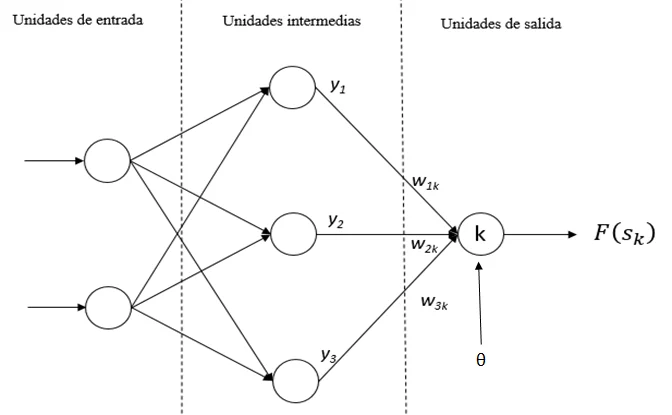
\includegraphics[width=0.7\linewidth]{figures/Simple_Neural_network.png}
    \caption{Esquema de una red neuronal simple. \citebox{firefly_ann_pretraining_researchgate_2026}}
    \label{fig: neural_network}
\end{figure}

Las funciones de activación más utilizadas en la práctica incluyen la sigmoide $\sigma(z) = 1/(1+e^{-z})$, la tangente hiperbólica $\sigma(z) = \tanh(z)$, y la unidad lineal rectificada (ReLU) $\sigma(z) = \max(0, z)$. La elección de la función de activación tiene consecuencias importantes sobre la dinámica del entrenamiento. Funciones como la sigmoide pueden producir gradientes que se desvanecen en redes profundas, mientras que la ReLU mitiga parcialmente este problema \citebox{schmidhuber2015deep}.

Una capa completa de la red consiste en $m$ neuronas que operan en paralelo sobre la misma entrada, produciendo un vector de salida $\mathbf{y} \in \mathbb{R}^m$:

\begin{equation} \label{eq: capa}
    \mathbf{y} = \sigma(\mathbf{W}\mathbf{x} + \mathbf{b})
\end{equation}

donde $\mathbf{W} \in \mathbb{R}^{m \times n}$ es la matriz de pesos de la capa y $\mathbf{b} \in \mathbb{R}^m$ el vector de sesgos.

Llegamos a la definición de \textit{deep learning}, que no es más que el uso de una red neuronal con muchas capas intermedias, lo que se conoce como red profunda. La expresión matemática que define una red profunda es una extensión de la\eqrefbox{eq: capa} pero para $L$ capas:

\begin{equation} \label{eq: red_profunda}
    f(\mathbf{x}) = \sigma_L(\mathbf{W}_L \cdots \sigma_2(\mathbf{W}_2 \, \sigma_1(\mathbf{W}_1 \mathbf{x} + \mathbf{b}_1) + \mathbf{b}_2) \cdots + \mathbf{b}_L)
\end{equation}

Los parámetros entrenables del modelo son el conjunto $\{\mathbf{W}_1, \mathbf{b}_1, \mathbf{W}_2, \mathbf{b}_2, \ldots, \mathbf{W}_L, \mathbf{b}_L\}$, cuyo número total crece con la anchura y la profundidad de la red.

El entrenamiento de una red neuronal se formula como un problema de optimización. Dado un conjunto de entrenamiento $\{(\mathbf{x}_n, y_n)\}_{n=1}^{N_T}$, se define una \textit{función de coste} (o función de pérdida) $C$ que mide la discrepancia entre las predicciones del modelo $f(\mathbf{x}_n)$ y las etiquetas verdaderas $y_n$. El objetivo es encontrar los parámetros $\boldsymbol{\theta} = \{\mathbf{W}_l, \mathbf{b}_l\}$ que minimizan $C$:

\begin{equation} \label{eq: optimizacion}
    \boldsymbol{\theta}^* = \arg\min_{\boldsymbol{\theta}} \; C(\boldsymbol{\theta}) = \arg\min_{\boldsymbol{\theta}} \; \frac{1}{N_T} \sum_{n=1}^{N_T} \mathcal{L}(f(\mathbf{x}_n; \boldsymbol{\theta}), y_n)
\end{equation}

donde $\mathcal{L}$ es una función de pérdida por muestra (por ejemplo, el error cuadrático medio o la entropía cruzada). Este es un problema de minimización en un espacio de alta dimensión, que se resuelve mediante variantes del \textit{descenso de gradiente} \citebox{schmidhuber2015deep}.

El algoritmo fundamental para calcular los gradientes necesarios es la \textit{backpropagation}, que aplica sistemáticamente la regla de la cadena del cálculo diferencial para propagar el error desde la capa de salida hacia las capas inferiores. Para un parámetro $\theta$ cualquiera de la red, el gradiente se calcula como:

\begin{equation} \label{eq: backprop}
    \frac{\partial C}{\partial \theta} = \frac{\partial C}{\partial \mathbf{y}_L} \cdot \frac{\partial \mathbf{y}_L}{\partial \mathbf{y}_{L-1}} \cdots \frac{\partial \mathbf{y}_{l+1}}{\partial \mathbf{y}_l} \cdot \frac{\partial \mathbf{y}_l}{\partial \theta}
\end{equation}

donde $\mathbf{y}_l$ es la salida de la capa $l$-ésima y cada factor $\partial \mathbf{y}_{l+1} / \partial \mathbf{y}_l$ es una matriz jacobiana, por lo que el orden de los productos es relevante. La actualización de los parámetros sigue entonces la regla $\theta \leftarrow \theta - \eta \, \partial C / \partial \theta$, donde $\eta > 0$ es la tasa de aprendizaje.

La diferencia fundamental entre las redes clásicas y las redes \textit{deep} radica en su capacidad de representación. Una red con una única capa oculta puede, en teoría, aproximar cualquier función continua con la suficiente anchura, pero resulta ineficiente para capturar estructuras jerárquicas, como las que están presentes en las imágenes o en el lenguaje natural \citebox{cybenko1989approximation, hornik1991approximation, cichocki2016tensor}. Las redes profundas, en cambio, aprenden representaciones en múltiples niveles de abstracción. Las capas más bajas detectan características primitivas como bordes o frecuencias, mientras que las superiores combinan estas primitivas para reconocer objetos complejos o conceptos semánticos \citebox{wang2023tensor}.

En clasificación de imágenes, las redes convolucionales han sido especialmente relevantes porque incorporan localidad espacial y pesos compartidos. Estas dos propiedades son adecuadas para datos visuales, porque los píxeles vecinos tienden a estar relacionados, y los mismos patrones pueden aparecer en distintas regiones de la imagen. La \figref{fig: 1} muestra algunas topologías básicas de redes neuronales.

\begin{figure}[H]
    \centering
    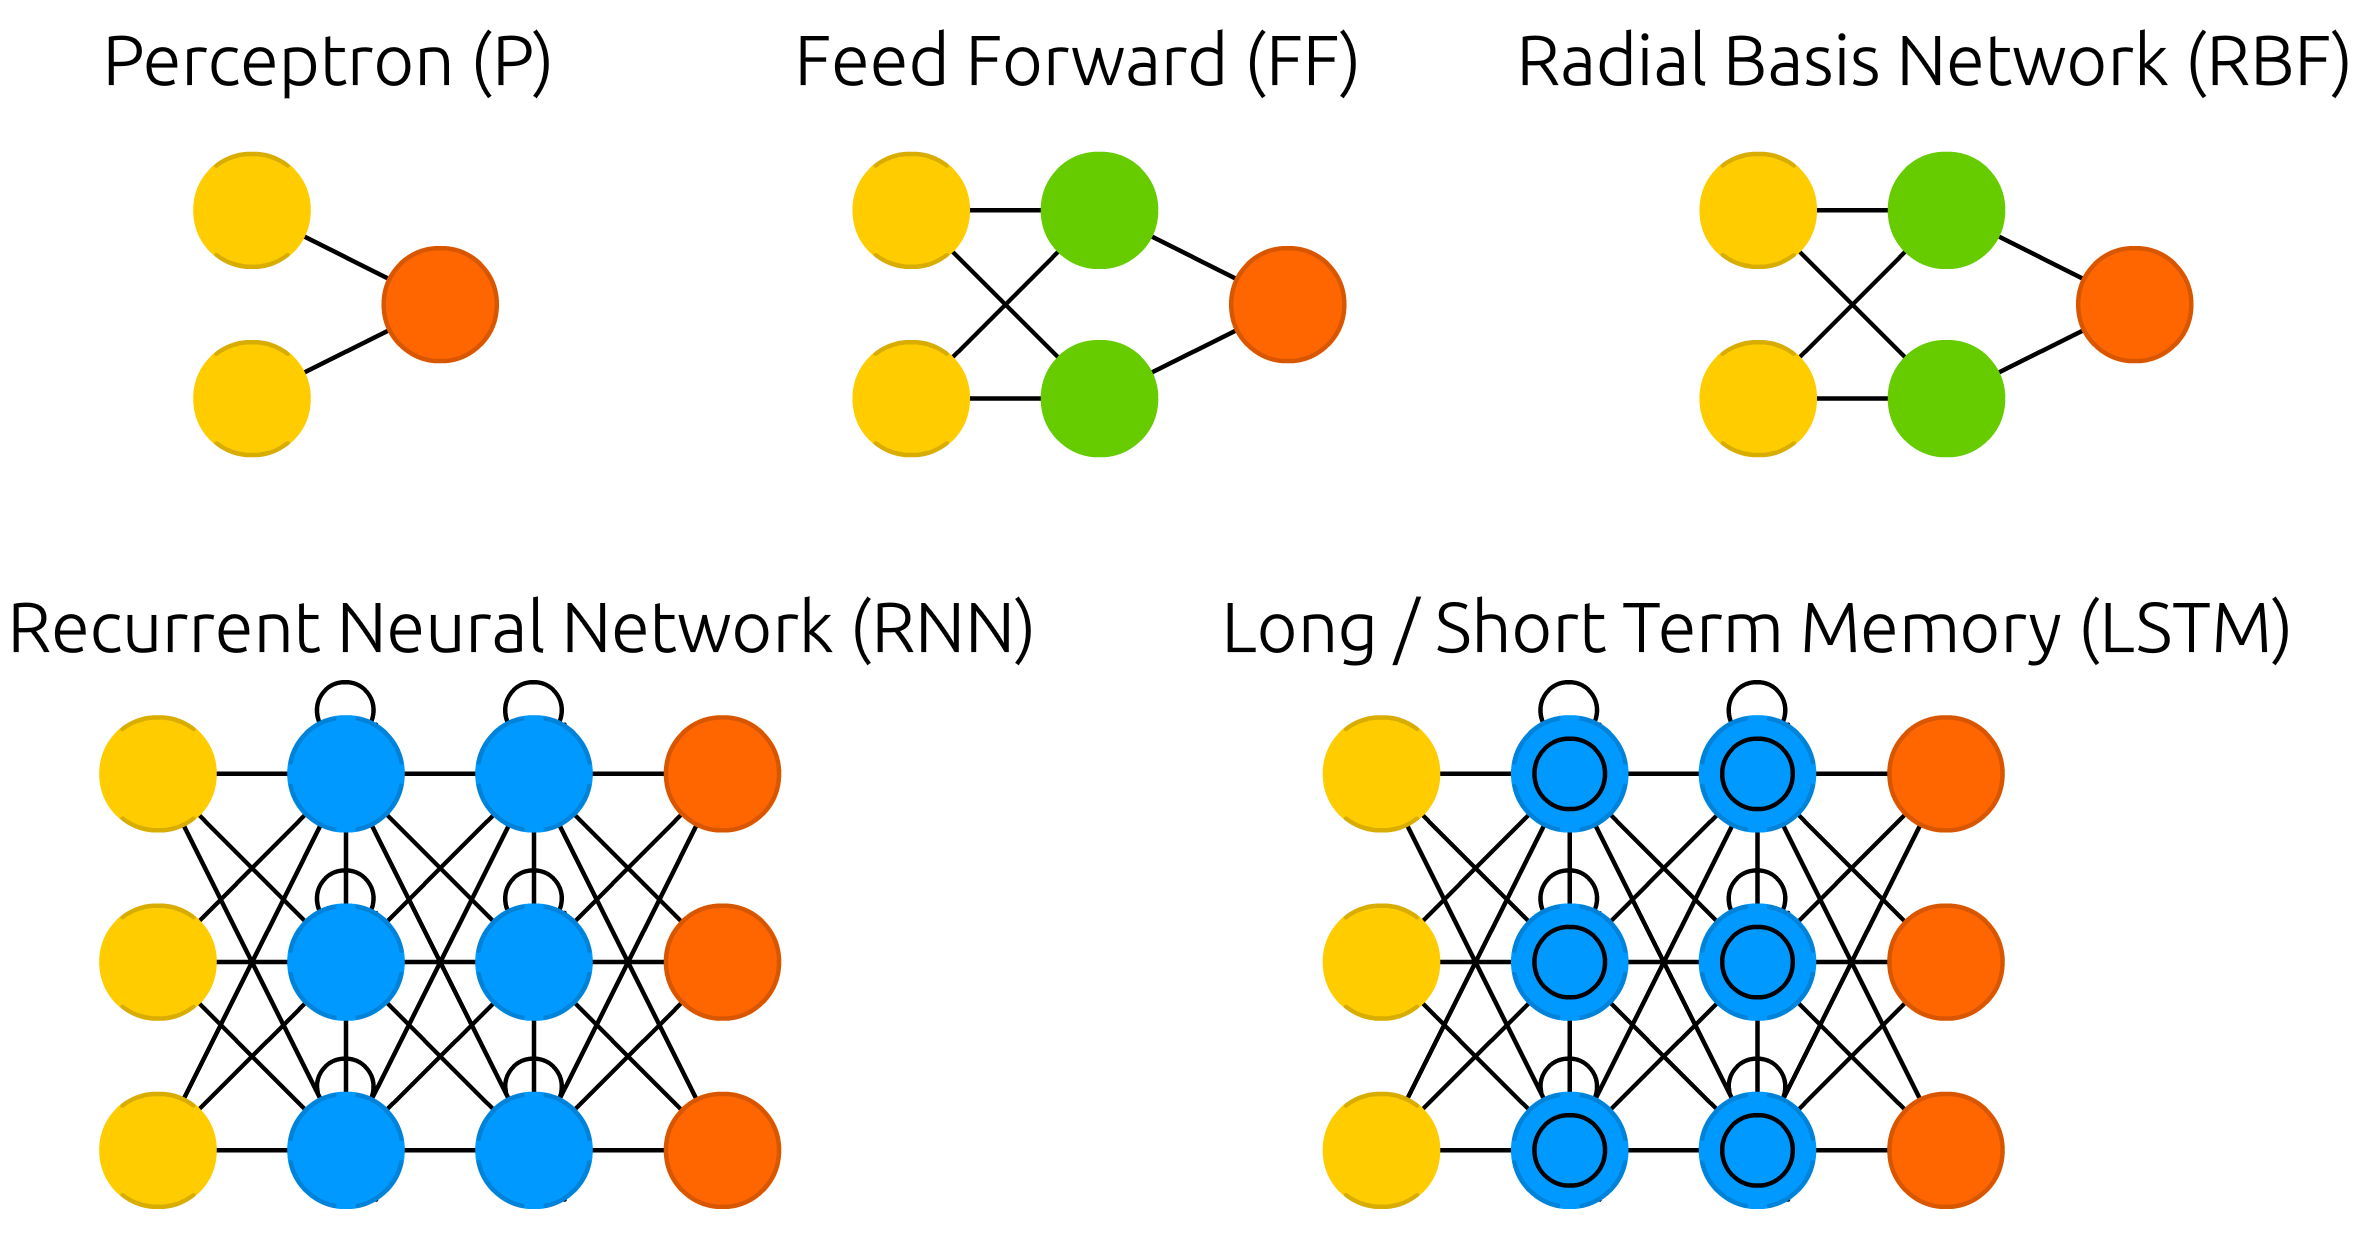
\includegraphics[width=0.78\linewidth]{figures/NeuralNetworks_recortada.png}
    \caption{Esquema de topologías básicas de redes neuronales, desde el perceptrón hasta arquitecturas con capas ocultas y conexiones recurrentes \citebox{vanveen2019zoo}.}
    \label{fig: 1}
\end{figure}

El éxito de estas arquitecturas no elimina sus limitaciones. Muchos modelos modernos alcanzan buenos resultados con un número elevado de parámetros y con un coste computacional considerable. Este TFG se sitúa en ese punto. Estudia si las TN pueden proporcionar modelos de clasificación estructurados, capaces de representar funciones complejas mediante factorizaciones tensoriales controladas.

\section{Tensores}

Antes de profundizar en el mundo de las TN es conveniente sentar primero las bases. Lo primero es entender qué es un tensor. Un tensor lo podemos ver definido de diferentes formas dependiendo del campo en el que estemos trabajando.

Desde un punto de vista computacional, los tensores son \textit{arrays} multidimensionales que generalizan de forma natural los conceptos de escalar, vector y matriz a dimensiones arbitrariamente superiores. Desde un punto de vista físico-matemático, los tensores son objetos matemáticos de orden superior, que representan relaciones multidimensionales entre distintas variables o grados de libertad. Dicho de otra forma, un tensor de orden $N$ es un objeto cuyos elementos tienen $N$ índices y están asociados a $N$ vectores base. \[R^{I_1 \times I_2 \times \cdots \times I_N}\] donde $N$ es el número de modos y las longitudes $I_1, \ldots, I_N$ representan las dimensiones de cada modo. \citebox{wang2023tensor}

Bajo esta definición, los escalares son tensores de orden cero, los vectores son tensores de orden 1, y las matrices son tensores de orden 2; todo caso superior constituye propiamente lo que en la literatura se denomina, tensor de alto orden. En la notación convencional, se distinguen los diferentes objetos según su orden: las letras minúsculas en cursiva ($a$) denotan escalares, las letras minúsculas en negrita ($\mathbf{a}$) denotan vectores, las letras mayúsculas en negrita ($\mathbf{A}$) denotan matrices, y las letras mayúsculas en tipografía cursiva en negrita ($\boldsymbol{\mathcal{A}}$) denotan tensores de orden superior. \citebox{wang2023tensor}

La intuición física detrás de los tensores resulta natural cuando se considera que muchos fenómenos del mundo real son inherentemente multidimensionales. Una imagen en color, por ejemplo, es un tensor de orden tres: altura, anchura y canales cromáticos. Los datos de resonancia magnética funcional (fMRI) constituyen tensores de orden cuatro. En mecánica cuántica, las funciones de onda de sistemas de muchos cuerpos son, igualmente, tensores de alto orden \citebox{wang2023tensor}.

El concepto de tensor tiene raíces en el siglo XIX, ligado al desarrollo del cálculo diferencial absoluto por Ricci-Curbastro y Levi-Civita, aunque fue la formulación de la relatividad general por Einstein en 1915 la que consagró los tensores como herramienta fundamental de la física matemática. La descripción matemática de un tensor es la siguiente:
\begin{equation} \label{eq: 1}
    \boldsymbol{\mathcal{T}} = \sum_{i_1, i_2,..., i_n} \tensor{T}{_{i_1}_{i_2}_{...}_{i_n}} \hat{b}_{i_1} \hat{b}_{i_2}...\hat{b}_{i_n}
\end{equation}

La operación central en el álgebra tensorial es la contracción tensorial. Dados dos tensores $\boldsymbol{\mathcal{T}}$ y $\boldsymbol{\mathcal{R}}$, de orden $n$ y $m$ respectivamente, con elementos $\tensor{T}{_{i_1}_{i_2}_{...}_{i_n}}$ y $\tensor{R}{_{j_1}_{j_2}_{...}_{j_m}}$ y en la misma base ortonormal $\hat{b}_{i}$, diremos que el tensor $\boldsymbol{\mathcal{C}}$ es la contracción de ambos tensores por sus últimos $q$ índices cuando:

\begin{equation} \label{eq: 2}
    \mathcal{C} = \sum_{i_1, i_2,...,i_{n-q},j_1,j_2,...,j_{m-q}} \tensor{C}{_{i_1}_{i_2}_{...}_{i_{n-q}}_{,}_{j_1}_{j_2}_{...}_{j_{m-q}}} \hat{b}_{i_1}\hat{b}_{i_2}...\hat{b}_{n-q}\hat{b}_{j_1}\hat{b}_{j_2}...\hat{b}_{m-q}
\end{equation}

siendo sus elementos

\begin{equation} \label{eq: 3}
    \tensor{C}{_{i_1}_{i_2}_{...}_{i_{n-q}}_{,}_{j_1}_{j_2}_{...}_{j_{m-q}}} = \sum_{k_1, k_2,...,k_{q}} \tensor{T}{_{i_1}_{i_2}_{...}_{i_{n-q}}_{,}_{k_1}_{k_2}_{...}_{k_{q}}} \tensor{R}{_{j_1}_{j_2}_{...}_{j_{m-q}}_{,}_{k_1}_{k_2}_{...}_{k_{q}}}
\end{equation}

De esta definición podemos sacar que la contracción tensorial es la operación mediante la cual dos tensores se contraen en un único tensor a lo largo de sus pares de índices asociados. Existen formas diferentes de contracciones, algunas implican más de dos tensores o un índice repetido en más de dos tensores o incluso repetidos en el mismo tensor. El caso más familiar de contracción tensorial es la multiplicación matricial: \[\mathbf{AB} = \sum_{k} A_{ik}B_{kj}\hat{b}_i\hat{b}_j\] o el producto escalar entre dos vectores: \[\mathbf{v}\cdot\mathbf{w} = \sum_i v_iw_i\]

Entre las operaciones tensoriales fundamentales cabe destacar la traza de una matriz:

\begin{equation}
    Tr(\mathbf{A}) = \sum_{i}A_{ii}
\end{equation}

Esto sería la contracción de una matriz consigo misma a través de sus índices repetidos. Debido a esta operación podemos ver que, un tensor también sirve como mapeo entre dos espacios vectoriales. Esto es un tensor, que recibe otro tensor y devuelve un tercer tensor. Por cada par de índices contraído estamos mezclando componentes de los tensores de entrada, reduciendo en 2 el orden total. Los índices que no han sido contraídos, en cambio, no desaparecen, sino que sobreviven como índices libres del tensor de salida. Así, al contraer un tensor de orden $n$ con uno de orden $m$ a lo largo de $q$ pares de índices, el tensor resultante tiene orden $n + m - 2q$, en consonancia con la \eqrefbox{eq: 3}.

\section{Notación diagramática de Penrose y definición de Tensor Network}

La representación algebraica de las contracciones tensoriales, aunque precisa, se vuelve rápidamente inmanejable a medida que aumenta el número de tensores y la complejidad de sus conexiones. Fue Roger Penrose \citebox{penrose1971applications} quien, a principios de la década de 1970, introdujo la notación diagramática para tensores, proporcionando una alternativa visual que transformó la manera en que se razona sobre estas estructuras. Los diagramas de redes tensoriales se utilizan hoy en día, en investigación, para describir algoritmos cuánticos y algoritmos de \textit{machine learning} \citebox{wang2023tensor}.

La idea central de la notación de Penrose es representar cada tensor como un nodo del que emanan tantas aristas como índices tenga el tensor. Concretamente, un nodo con una sola arista representa un vector $\mathbf{a} \in \mathbb{R}^I$; un nodo con dos aristas representa una matriz $\mathbf{A} \in \mathbb{R}^{I \times J}$; y un nodo con tres aristas representa un tensor $\boldsymbol{\mathcal{A}} \in \mathbb{R}^{I_1 \times I_2 \times I_3}$. Para indicar que un par de índices tensoriales está siendo contraído, ambas aristas se unen mediante una línea. Por ejemplo, la contracción de un tensor de orden uno con uno de orden dos es la multiplicación matriz-vector habitual. Las aristas que no se conectan a ningún otro tensor se denominan aristas libres, y el número de estas aristas en el diagrama resultante es precisamente el orden del tensor final. Dos nodos que no están unidos mediante aristas, representan el producto tensorial entre ellos.

\begin{figure}[H]
    \centering
    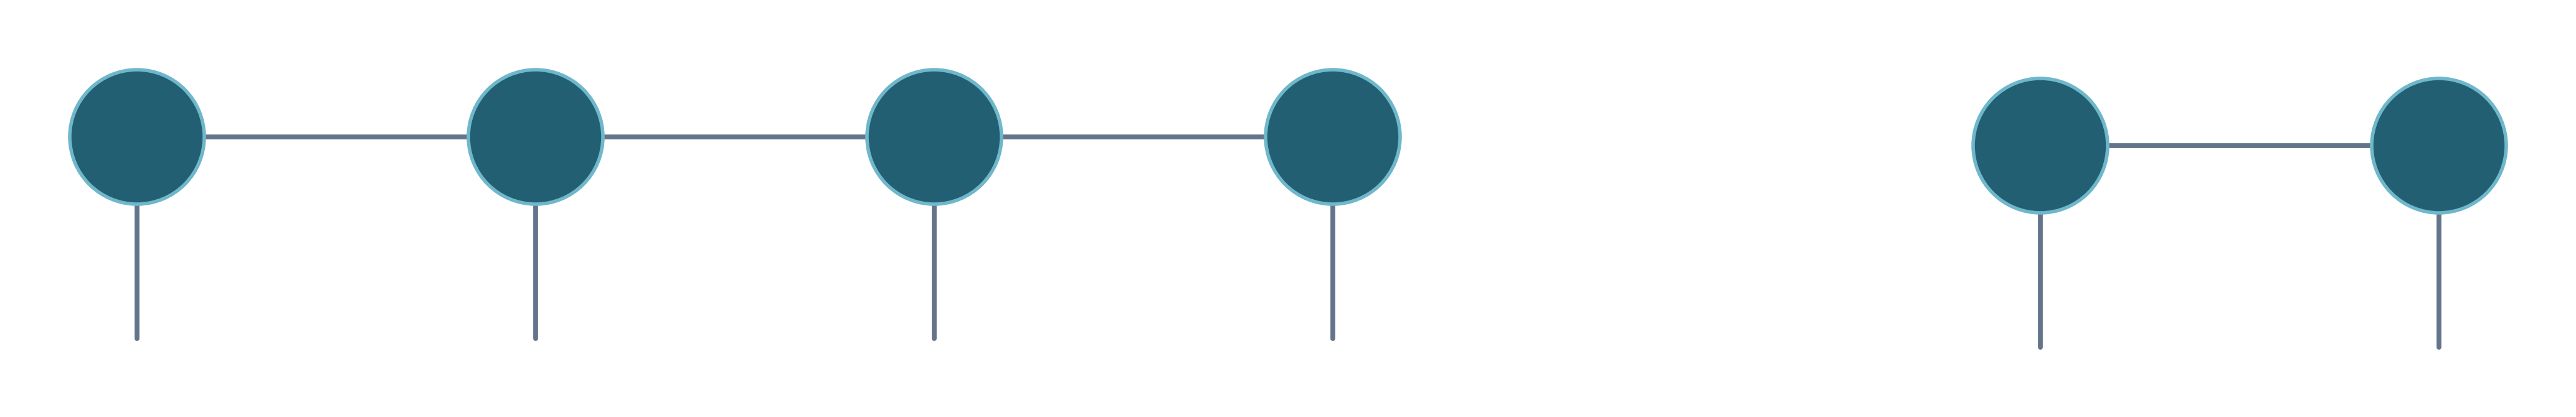
\includegraphics[width=1.0\linewidth]{figures/TN_invented.png}
    \caption{Representación de una TN inventada. En esta representación se pueden identificar muchas de las operaciones descritas en esta sección. Elaboración propia usando la librería Tensor-Network-Editor, creada por Alejandro Mata Ali. \citebox{Mata_Ali_Tensor_Network_Editor_2026}}
    \label{fig:Invented_TN}
\end{figure}

La notación gráfica tensorial ofrece numerosas ventajas sobre la notación tradicional. En forma gráfica, los índices no necesitan nombres ni etiquetas; operaciones como el producto escalar, la traza tensorial y la contracción pueden expresarse sin notación adicional; y el orden del tensor resultante puede leerse simplemente contando el número de aristas libres. En particular, si en el diagrama no quedan aristas libres tras todas las contracciones, el resultado es necesariamente un escalar. Esta propiedad convierte los diagramas en una herramienta de verificación inmediata de la consistencia dimensional de operaciones complejas \citebox{stoudenmire2017supervisedlearningquantuminspiredtensor}. Sobre esta base visual puede introducirse ya, de manera natural, el concepto de \textit{Tensor Network (TN)}.

Una TN es, en esencia, una representación gráfica de una ecuación multilineal entre diferentes tensores. Esta representación se apoya en la notación diagramática de Penrose, que con el tiempo se ha ido adaptando a las necesidades de disciplinas como la física, las matemáticas o la ciencia computacional \citebox{biamonte2017tensornetworksnutshell}. Puede verse un ejemplo en la \figref{fig: TensorNetwork}, donde aparece la TN que representa el 2-tensor $\tensor{T}{_{i}_{p}}$ cuyos elementos se obtienen mediante la operación de contracción

\begin{equation} \label{eq: 5}
\tensor{T}{_{i}_{p}} = \sum_{j, k, l, m, n, o}\tensor{A}{_{i}_{j}_{k}_{l}} \tensor{B}{_{j}_{m}}\tensor{C}{_{k}_{m}_{n}}\tensor{D}{_{l}_{o}}\tensor{E}{_{n}_{o}_{p}}
\end{equation}

\begin{figure}[H]
\centering
\makebox[\textwidth]{%
  \begin{minipage}{1.1\textwidth}
    \centering
    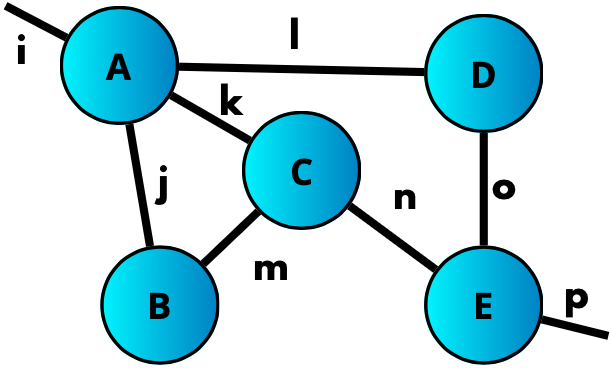
\includegraphics[scale=0.45]{figures/TensorNetwork_example.png}
    \caption{Ejemplo de representación diagramática para un tensor. Fuente:\citebox{2024arXiv240411277M}}
    \label{fig: TensorNetwork}
  \end{minipage}%
}
\end{figure}

Desde un punto de vista computacional, una Tensor Network no debe entenderse únicamente como un dibujo, sino como una forma factorizada de representar un tensor de alto orden. En lugar de almacenar explícitamente todos los elementos del tensor completo, se almacena una colección de tensores de menor orden, conectados entre sí mediante índices compartidos. Cada tensor de la red suele denominarse también núcleo, bloque o tensor local, dependiendo del contexto \citebox{wang2023tensor}.

En una red tensorial aparecen dos tipos de índices con papeles distintos. Los índices que quedan libres tras realizar las contracciones corresponden a los índices del tensor final representado por la red. En problemas de física cuántica suelen denominarse índices físicos, mientras que en aplicaciones de aprendizaje automático pueden interpretarse como posiciones de entrada, características o salidas del modelo. Por otro lado, los índices que conectan dos tensores internos se denominan índices virtuales o índices de enlace. Estos índices no aparecen en el tensor final, ya que se suman durante la contracción, pero controlan cuánta información puede transmitirse entre distintas partes de la red.

La dimensión de estos índices internos, denominada dimensión de enlace, es uno de los parámetros más importantes de una Tensor Network. Si la dimensión de enlace es pequeña, la red contiene pocos parámetros y la representación es muy compacta, pero también queda limitada su capacidad para representar correlaciones complejas. Si la dimensión de enlace aumenta, la red gana expresividad, aunque también crecen el número de parámetros y el coste computacional de las contracciones. Por tanto, la dimensión de enlace desempeña un papel análogo al de un hiperparámetro que regula el compromiso entre compacidad y capacidad de representación.

La operación fundamental en una Tensor Network es la contracción. Contraer una red significa sumar sobre todos los índices internos compartidos hasta obtener el tensor final, que queda determinado únicamente por sus índices libres. Aunque algebraicamente esta operación puede escribirse como una suma sobre muchos índices, la notación diagramática permite visualizarla de forma más intuitiva; las aristas conectadas se eliminan al contraerse, mientras que las aristas libres permanecen como índices del resultado. Además, el orden en el que se realizan las contracciones puede afectar de forma significativa al coste computacional, por lo que una misma red puede ser más o menos eficiente dependiendo de la estrategia de contracción empleada \citebox{wang2023tensor}.

\section{Tensor Networks y reducción de dimensionalidad}

La motivación fundamental para el uso de las Tensor Networks es de naturaleza computacional. Un tensor de orden $N$ cuyos índices toman cada uno $d$ valores posee $d^N$ componentes, un número que crece exponencialmente con el orden del tensor y que hace inviable su almacenamiento y manipulación directos incluso para valores moderados de $N$ y $d$. Este fenómeno se conoce como \textit{maldición de la dimensionalidad} \citebox{wang2023tensor}.

El mismo problema aparece de forma natural en la física cuántica de muchos cuerpos, que es precisamente el contexto en el que surgieron las TN. Un estado cuántico general de $N$ subsistemas con dimensión local $d$ se escribe como

\begin{equation} \label{eq: estado_general}
    \ket{\psi} =
    \sum_{s_1,\ldots,s_N}
    C_{s_1\ldots s_N}\,
    \ket{s_1}\otimes\cdots\otimes\ket{s_N},
\end{equation}

donde el tensor de coeficientes $C_{s_1\ldots s_N}$ tiene de nuevo $d^N$ componentes. Sin embargo, los estados físicamente relevantes rara vez ocupan todo ese espacio con la máxima complejidad posible, porque sus correlaciones y su entrelazamiento suelen estar limitados, lo que permite representarlos de forma mucho más compacta de lo que sugiere el conteo $d^N$ \citebox{schollwock2011dmrg}.

La idea central de las Tensor Networks consiste en aprovechar esa estructura. En lugar de almacenar explícitamente el tensor completo, se representa como el resultado de contraer un conjunto de tensores de menor orden conectados entre sí mediante índices de enlace. Si las dimensiones de esos índices internos se mantienen acotadas, el número total de parámetros crece de forma polinómica e incluso lineal en algunas topologías, en lugar de exponencial con el número de modos \citebox{wang2023tensor, stoudenmire2017supervisedlearningquantuminspiredtensor}.

Esta reducción no es gratuita. Al fijar una topología concreta y unas dimensiones de enlace finitas se restringe la familia de tensores que pueden representarse de forma eficiente. Por ello, una Tensor Network debe entenderse como una aproximación estructurada; solo resulta eficaz cuando la estructura de correlaciones del problema es compatible con la topología elegida. Esta distinción es especialmente importante en \textit{machine learning}, donde la red tensorial no se limita a comprimir un tensor ya conocido, sino que se utiliza como una arquitectura entrenable cuyos parámetros se ajustan a partir de los datos.

Esta observación se traslada al \textit{machine learning} mediante una analogía útil. Un modelo de clasificación no necesita representar una función arbitraria sobre todas las entradas posibles, sino una función que aproveche las regularidades de los datos. Las Tensor Networks imponen una estructura de bajo rango o de conectividad concreta sobre el tensor de pesos, de modo que el número de parámetros permanece controlado siempre que las dimensiones internas, llamadas dimensiones de enlace, se mantengan acotadas \citebox{cichocki2016tensor, wang2023tensor}.

\section{Descomposiciones tensoriales fundamentales}

Para comprender cómo se construyen las representaciones mediante TN, conviene introducir primero algunas descomposiciones tensoriales básicas. Cada una puede entenderse como una forma distinta de imponer estructura sobre un tensor de alto orden. La descomposición CP lo expresa como una suma de términos separables; la de Tucker introduce un núcleo central que acopla varios factores; y el formato Tensor Train (TT), conocido en física como Matrix Product State (MPS), organiza la información en una cadena de tensores conectados por índices de enlace. Cada uno ofrece un compromiso diferente entre compacidad, expresividad y coste computacional, como se verá a lo largo de la sección.

La herramienta algebraica fundamental es la descomposición en valores singulares (SVD). Dada una matriz $\mathbf{A} \in \mathbb{R}^{M \times N}$, la SVD la factoriza como

\begin{equation} \label{eq: svd}
    \mathbf{A} = \mathbf{U} \boldsymbol{\Sigma} \mathbf{V}^\top ,
\end{equation}

donde $\mathbf{U}$ y $\mathbf{V}$ son matrices ortogonales, y $\boldsymbol{\Sigma}$ contiene los valores singulares $\sigma_1 \geq \sigma_2 \geq \cdots \geq 0$. La importancia de la SVD en TN se debe a que permite obtener la mejor aproximación de bajo rango en norma de Frobenius. Al conservar solo los $R$ valores singulares dominantes se obtiene la matriz de rango $R$ que minimiza el error de reconstrucción, resultado conocido como teorema de Eckart--Young \citebox{wang2023tensor}.

Una primera generalización del rango matricial a tensores de orden superior es la descomposición CP. Dado un tensor $\boldsymbol{\mathcal{X}} \in \mathbb{R}^{I_1 \times \cdots \times I_N}$, CP lo aproxima como suma de $R$ tensores de rango 1:

\begin{equation} \label{eq: CP}
    \boldsymbol{\mathcal{X}} \approx \sum_{r=1}^{R} 
    \mathbf{a}_r^{(1)} \circ \mathbf{a}_r^{(2)} \circ \cdots \circ \mathbf{a}_r^{(N)} ,
\end{equation}

donde $\circ$ denota el producto exterior y $R$ es el rango CP. Esta representación es muy compacta, con $R \sum_{n=1}^{N} I_n$ parámetros, pero presenta dificultades prácticas; determinar el rango CP es un problema NP-difícil y los métodos de ajuste habituales no garantizan alcanzar el óptimo global \citebox{kolda2009tensor, wang2023tensor}. En notación diagramática, CP se representa mediante factores vectoriales conectados a un nodo central diagonal.

La descomposición de Tucker es más flexible. En lugar de una única suma de componentes de rango 1, introduce un tensor núcleo $\boldsymbol{\mathcal{G}}$ que modela las interacciones entre los factores:

\begin{equation} \label{eq: Tucker}
    \tensor{\mathcal{X}}{_{i_1}_{i_2}_{...}_{i_N}} \approx 
    \sum_{r_1=1}^{R_1} \cdots \sum_{r_N=1}^{R_N}
    \tensor{\mathcal{G}}{_{r_1}_{r_2}_{...}_{r_N}}
    \tensor{A}{^{(1)}_{i_1 r_1}}
    \tensor{A}{^{(2)}_{i_2 r_2}}
    \cdots
    \tensor{A}{^{(N)}_{i_N r_N}} .
\end{equation}

Los valores $R_1,\ldots,R_N$ son los rangos de Tucker y pueden ser distintos para cada modo. Si las matrices de factores son ortogonales, se obtiene la Higher-Order Singular Value Decomposition (HOSVD), una extensión natural de la SVD al caso tensorial \citebox{wang2023tensor}. CP puede verse como un caso particular de Tucker cuando el núcleo es superdiagonal y todos los rangos coinciden. Sin embargo, el núcleo de Tucker contiene $\prod_{n=1}^{N} R_n$ parámetros, por lo que el coste vuelve a crecer exponencialmente con el orden del tensor.

Esta limitación motiva formatos más escalables como Tensor Train (TT), conocido en física como Matrix Product State (MPS) \citebox{oseledets2011tt, schollwock2011dmrg}. TT representa un tensor de orden $N$ como una cadena de tensores locales $\boldsymbol{\mathcal{G}}^{(n)} \in \mathbb{R}^{R_{n-1} \times I_n \times R_n}$ conectados mediante índices virtuales. Su número de parámetros es

\[
    \sum_{n=1}^{N} R_{n-1} I_n R_n ,
\]

que crece linealmente con $N$ si los rangos se mantienen acotados. Además, la descomposición TT puede construirse mediante SVD sucesivas, lo que proporciona estabilidad numérica y permite controlar el error mediante el truncamiento de valores singulares \citebox{wang2023tensor, oseledets2011tt}. Desde la perspectiva cuántica, los rangos TT coinciden con los rangos de Schmidt de las biparticiones correspondientes, conectando esta construcción con la noción de entrelazamiento discutida anteriormente \citebox{schollwock2011dmrg}.

La \tabref{tab:comparativa_descomposiciones} resume las diferencias principales entre los formatos anteriores.

\begin{table}[H]
\centering
\renewcommand{\arraystretch}{1.3}

\begin{tabularx}{\textwidth}{|l|c|X|}
\hline
\textbf{Formato} & \textbf{Parámetros} & \textbf{Observaciones} \\
\hline
CP &
$R \sum_n I_n$ &
Muy compacta, pero el rango CP es difícil de determinar. \\
\hline
Tucker &
$\prod_n R_n + \sum_n I_n R_n$ &
Flexible, pero el núcleo crece exponencialmente con el orden. \\
\hline
TT/MPS &
$\sum_n R_{n-1} I_n R_n$ &
Escalado lineal para rangos fijos; construible mediante SVD sucesivas. \\
\hline
\end{tabularx}

\caption{Comparación entre las descomposiciones CP, Tucker y TT/MPS.}
\label{tab:comparativa_descomposiciones}
\end{table}

\begin{figure}[H]
    \centering
    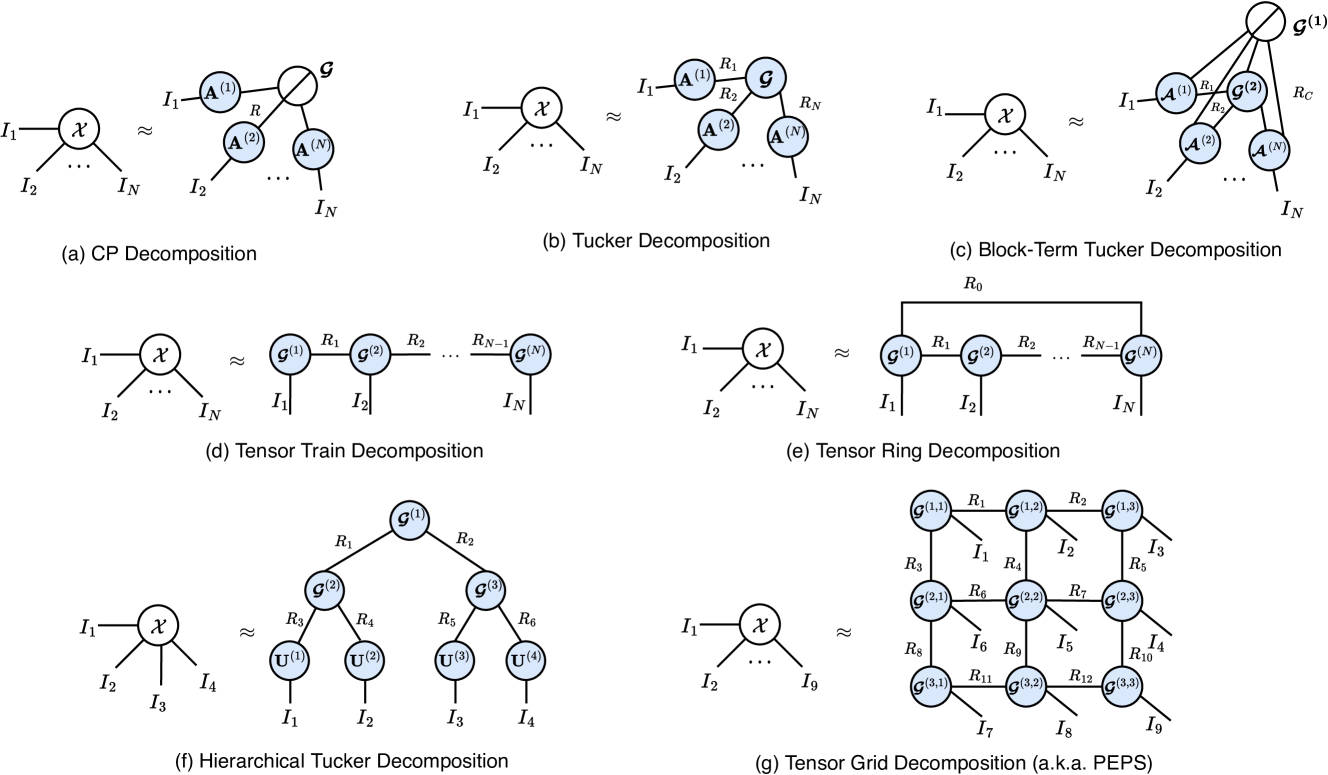
\includegraphics[width=0.9\linewidth]{figures/Decompositions_in_TN.png}
    \caption{Diagramas TN de algunas descomposiciones tensoriales populares. (a) El formato CP descompone un tensor \(X\) en una suma de varios tensores de rango 1 $a^{(1)}_{:,r} \circ a^{(2)}_{:,r} \circ \cdots \circ a^{(N)}_{:,r}.$ (b) La descomposición de Tucker descompone un tensor \(X\) en un tensor núcleo \(G\) multiplicado por una matriz \(A^{(n)}\) a lo largo del modo \(n\)-ésimo. (d) La descomposición TT descompone un tensor \(X\) en una multiplicación lineal de un conjunto de tensores núcleo de tercer orden $G^{(2)} \cdots G^{(N-1)}$ y dos matrices \(G^{(1)}\) y \(G^{(N)}\). (g) La descomposición en malla tensorial, también conocida como PEPS, representa un tensor de alta dimensión como una malla bidimensional de tensores interconectados de menor rango, donde cada nodo se conecta con sus vecinos para capturar eficientemente correlaciones espaciales en sistemas con interacciones locales. Los paneles (c), (e) y (f) corresponden, respectivamente, a las descomposiciones en términos de bloque, Tensor Ring (TR) y jerárquica de Tucker (HT), no empleadas en este trabajo. \citebox{wang2023tensor}}
    \label{fig: cp_decomposition}
\end{figure}

\section{Topologías principales de Tensor Networks}

La topología de una Tensor Network determina qué correlaciones puede representar de forma eficiente y con qué coste computacional. En esta sección se detallan las topologías de TN más utilizadas y más relevantes en la literatura.

\subsection{Matrix Product State / Tensor Train}

El \textit{Matrix Product State} (MPS), conocido en la literatura matemática como Tensor Train (TT), es la topología de TN más estudiada y mejor comprendida. Consiste en una cadena lineal de $N$ tensores conectados secuencialmente mediante índices virtuales de dimensión $D$. Los tensores de los extremos tienen dos índices y los intermedios tres, un índice asociado a la posición de entrada y dos índices de enlace que conectan con los vecinos. Ambos nombres describen la misma topología y la diferencia está en el contexto de uso. En física la MPS se introdujo para representar estados cuánticos de muchos cuerpos, mientras que en análisis numérico y aprendizaje automático el formato TT se emplea como herramienta de compresión y parametrización eficiente de tensores de alta dimensión \citebox{oseledets2011tt}.

Los índices internos de la cadena reciben el nombre de rangos TT o dimensiones de enlace, y determinan cuánta información puede transmitirse entre las distintas partes de la cadena. Dimensiones pequeñas dan un modelo muy compacto pero con capacidad limitada para representar correlaciones entre posiciones alejadas; al aumentarlas, la representación gana expresividad a costa de más parámetros y contracciones más costosas. En aplicaciones de aprendizaje automático, la dimensión de enlace actúa por tanto como un hiperparámetro que regula la complejidad del modelo \citebox{stoudenmire2017supervisedlearningquantuminspiredtensor}.

Una ventaja relevante del formato TT es que puede construirse aplicando descomposiciones en valores singulares de forma sucesiva a distintas matricizaciones del tensor. Este procedimiento, conocido como TT-SVD, proporciona una forma numéricamente estable de obtener una aproximación con rangos controlados \citebox{oseledets2011tt}, y conecta la MPS con la SVD introducida anteriormente: no es solo una arquitectura inspirada en la física, sino también una herramienta de reducción de dimensionalidad.

Desde el punto de vista físico, la MPS es la representación más natural de los estados fundamentales de los sistemas cuánticos unidimensionales con interacciones locales, lo que explica su relevancia en este campo. Una propiedad característica es que las correlaciones que puede representar decaen exponencialmente con la distancia entre posiciones: la función de correlación entre las posiciones $i$ y $j$ satisface:

\begin{equation}
  \langle O_i O_j \rangle - \langle O_i \rangle \langle O_j \rangle \sim e^{-|i-j|/\xi}   
\end{equation}

donde $\xi$ es una longitud de correlación que depende de la dimensión de enlace $D$ \citebox{stoudenmire2017supervisedlearningquantuminspiredtensor}. Por ello la MPS captura con eficiencia las correlaciones de corto alcance, pero puede requerir dimensiones de enlace elevadas para las de largo alcance.

No obstante, la MPS organiza la información en una cadena. Esto es natural para datos secuenciales, pero menos adecuado para imágenes, que poseen una estructura espacial bidimensional. Aplicar una MPS a una imagen obliga a ordenar sus posiciones de entrada en una secuencia. Esa ordenación puede conservar parcialmente la vecindad espacial, por ejemplo mediante un recorrido en zigzag, pero transforma inevitablemente una geometría bidimensional en una unidimensional. Esta limitación es una de las motivaciones para considerar topologías jerárquicas, como las Tree Tensor Networks, en problemas de visión artificial.

Una forma especialmente interesante de utilizar una MPS en aprendizaje supervisado consiste en emplearla como parametrización del tensor de pesos de un clasificador. En un modelo lineal convencional, la entrada se representa mediante un vector de características que se multiplica por una matriz de pesos. En el enfoque tensorial, la entrada se transforma primero en un tensor de alto orden mediante un mapa local de características y el tensor de pesos se representa de forma comprimida mediante una MPS \citebox{stoudenmire2017supervisedlearningquantuminspiredtensor}. De manera esquemática, si una entrada $x$ se descompone en varias posiciones $x_1,\ldots,x_N$, a cada una se le aplica un mapa local

\[ \phi(x_j) \in \mathbb{R}^{d}, \]

con $d$ la dimensión local, y la representación completa de la entrada se obtiene como producto tensorial de todos los vectores locales:

\[ \Phi(x)=\phi(x_1)\otimes \phi(x_2)\otimes \cdots \otimes \phi(x_N). \]

Aunque formalmente $\Phi(x)$ pertenece a un espacio de dimensión $d^N$, no es necesario construirlo de forma explícita, porque la estructura de la red permite trabajar con esta representación de manera implícita mediante contracciones sucesivas. Para clasificación multiclase se introduce un índice adicional asociado a la etiqueta de clase, de modo que la MPS representa un tensor de pesos $W^{\ell}$ y, al contraerlo con la representación de entrada, se obtiene una puntuación por clase:

\[ f^{\ell}(x)= W^{\ell}\cdot \Phi(x). \]

La clase predicha es la de mayor puntuación. En el lenguaje habitual del \textit{deep learning}, estas puntuaciones se interpretan como los valores previos a la normalización probabilística final del clasificador. Así, la MPS no se limita a comprimir un tensor ya conocido, sino que define directamente la forma de los parámetros que se optimizan, y su dimensión de enlace controla la complejidad del clasificador.

Este esquema fue explorado por Stoudenmire y Schwab, que aplicaron una MPS a la clasificación de dígitos manuscritos sobre MNIST, ordenando los píxeles en una secuencia mediante un recorrido en zigzag para preservar en parte la proximidad espacial, y alcanzaron un error de test inferior al $1\%$ \citebox{stoudenmire2017supervisedlearningquantuminspiredtensor}. Este resultado ilustra el potencial de la MPS como clasificador entrenable, pero también se hace evidente la necesidad de linealizar una imagen bidimensional antes de introducirla en la red, que es su gran limitación.

\subsection{Tree Tensor Network}

Una \textit{Tree Tensor Network} (TTN) organiza los tensores siguiendo una estructura jerárquica en forma de árbol. En lugar de propagar la información a lo largo de una cadena, asocia los tensores de la capa más baja (las \textit{hojas} o \textit{leaves} en inglés) a las posiciones de entrada y los contrae por grupos hacia tensores de capas superiores, reduciendo progresivamente el número de índices hasta llegar a un único tensor raíz que produce la salida. Los tensores de los niveles inferiores combinan información local, mientras que los superiores integran representaciones cada vez más globales, de modo que la red construye una jerarquía de características sobre la que se realiza la clasificación.

La diferencia esencial con una MPS es la forma en que se propagan las dependencias entre posiciones de entrada. En una cadena, dos posiciones alejadas solo se comunican a través de todos los tensores intermedios; en un árbol, en cambio, basta ascender unos pocos niveles hasta un nodo común, de manera que la distancia efectiva entre dos hojas crece como $\mathcal{O}(\log N)$ en lugar de linealmente \citebox{wang2023tensor, evenbly2011tensor}. Esta geometría hace que la TTN sea más eficiente que la MPS para combinar información lejana y, por tanto, para capturar correlaciones de largo alcance.

Al igual que en una MPS, la dimensión de los índices internos regula el compromiso entre compacidad y expresividad. Si es demasiado pequeña, la red pierde información relevante durante la compresión jerárquica; si es demasiado grande, gana capacidad pero aumentan el número de parámetros y el coste de entrenamiento. Existe, además, una decisión estructural que no es neutra: la forma concreta del árbol fija de antemano qué grupos de entradas se combinan primero y cuáles solo se encuentran en niveles superiores, lo que condiciona el tipo de dependencias que el modelo representa con mayor facilidad. En problemas de imágenes esta cuestión es especialmente relevante, ya que la organización espacial de la entrada influye en qué regiones conviene agrupar antes.

En física, la TTN se emplea para representar estados con una estructura de entrelazamiento jerárquica, como la que aparece en ciertos sistemas con simetría de escala. En \textit{machine learning}, su organización en árbol resulta natural para datos con estructura jerárquica intrínseca \citebox{wang2023tensor}. Esta correspondencia es la que motiva su uso en este trabajo. Aunque una TTN no reproduce de forma exacta la geometría bidimensional de una imagen, sí ofrece un mecanismo para agrupar posiciones de entrada y combinar la información de manera progresiva. Por ello la TTN no se aplica aquí directamente sobre los píxeles, sino sobre una secuencia de vectores de características obtenida tras una etapa inicial de extracción visual, un planteamiento híbrido que se detalla en la metodología.

La estructura de árbol también introduce una limitación. Al no contener ciclos, la información entre dos ramas distintas solo puede propagarse a través de su nodo ancestro común, lo que restringe la capacidad de la red para capturar correlaciones entre nodos situados en ramas separadas. Esta restricción es la que motivó el desarrollo de arquitecturas más sofisticadas como la MERA.

\subsection{MERA}

La \textit{Multi-scale Entanglement Renormalization Ansatz} (MERA) fue introducida por Vidal en 2007 como una Tensor Network capaz de representar eficientemente los estados fundamentales de sistemas cuánticos en los que las correlaciones decaen como una ley de potencias en lugar de exponencialmente \citebox{vidal2007mera}. Puede entenderse como una extensión de las redes jerárquicas tipo árbol: al igual que una TTN, organiza la información en niveles sucesivos, pero introduce un elemento adicional característico, los \textit{disentanglers} (desentrelazadores).

En cada capa de la estructura jerárquica, antes de reducir el número de grados de libertad, los disentanglers actúan sobre pares de posiciones vecinas para eliminar el entrelazamiento de corto alcance. A continuación, los tensores de renormalización (isometrías) agrupan varios grados de libertad en una representación más compacta y capturan las correlaciones a escalas mayores. La alternancia de capas de disentanglers y de renormalización es lo que permite a la MERA representar correlaciones a todas las escalas de longitud simultáneamente \citebox{vidal2007mera, wang2023tensor}.

Esta organización está estrechamente relacionada con el grupo de renormalización. Cada capa puede interpretarse como una descripción efectiva del sistema a una escala de longitud distinta, de las más locales en los niveles inferiores a las más globales en los superiores. En esta lectura, mientras una MPS reproduce esencialmente la geometría unidimensional de la cadena, la MERA introduce una geometría adicional asociada a la escala, que conecta posiciones alejadas a través de sus capas superiores \citebox{evenbly2011tensor}. Por ello, donde una MPS podría requerir una dimensión de enlace que crece con el tamaño del sistema, la estructura multiescala de la MERA captura estas correlaciones de forma más natural.

En \textit{machine learning}, esta capacidad para tratar dependencias a múltiples escalas resulta sugerente para datos como las imágenes, que contienen patrones organizados a distintos niveles. Sin embargo, la presencia de disentanglers y el mayor coste de sus contracciones hacen que la MERA sea bastante más compleja de implementar y entrenar que una MPS o una TTN. Por esta razón, en este trabajo se considera principalmente como una topología relevante desde el punto de vista teórico, mientras que la implementación experimental se apoya en una arquitectura jerárquica basada en TTN, situada así dentro de una familia más amplia de redes tensoriales jerárquicas.
 
\subsection{PEPS}

Los \textit{Projected Entangled Pair States} (PEPS) son la generalización más natural del MPS a dos dimensiones. Mientras que en la topología MPS cada tensor se conecta a lo sumo con dos vecinos, en PEPS cada tensor se conecta con cuatro vecinos, formando una red bidimensional que refleja directamente la geometría de una rejilla cuadrada \citebox{verstraete2004peps}.

Para un sistema bidimensional de $M \times N$ sitios, cada tensor local en PEPS tiene un índice físico de dimensión $d$ y cuatro índices virtuales (arriba, abajo, izquierda, derecha) de dimensión $D$. Esto permite capturar de forma natural las correlaciones espaciales bidimensionales que caracterizan, por ejemplo, los estados fundamentales de sistemas cuánticos definidos sobre rejillas planas \citebox{wang2023tensor}.
 
Sin embargo, esta ventaja geométrica tiene un coste. La contracción exacta de una red PEPS es un problema computacionalmente intratable, concretamente \#P-difícil \citebox{schuch2007computationalcomplexitypeps}; a diferencia del MPS, donde la contracción exacta tiene un coste polinomial. En la práctica, esto obliga a utilizar métodos de contracción aproximada, lo que introduce errores adicionales y limita el tamaño de las dimensiones de enlace que pueden utilizarse \citebox{wang2023tensor}. Existen aplicaciones de PEPS a clasificación supervisada en conjuntos como MNIST y Fashion-MNIST \citebox{cheng2021supervisedlearningpeps}.

\begin{table}[H]
\centering
\renewcommand{\arraystretch}{1.3}
\begin{tabularx}{\textwidth}{|l|c|X|X|}
\hline
\textbf{Topología} & \textbf{Parámetros típicos} & \textbf{Ventaja principal} & \textbf{Limitación práctica} \\
\hline
MPS / TT & $\mathcal{O}(NdD^2)$ & Contracción eficiente y literatura consolidada. & Geometría 1D para datos que pueden ser 2D. \\
\hline
TTN & $\mathcal{O}(ND^3)$ & Agregación jerárquica y distancia logarítmica. & Interacciones limitadas entre ramas separadas. \\
\hline
PEPS & $\mathcal{O}(NdD^4)$ & Geometría 2D natural. & Contracción exacta intratable en general. \\
\hline
MERA & $\mathcal{O}(ND^4)$ & Correlaciones multiescala. & Mayor complejidad estructural y computacional. \\
\hline
\end{tabularx}
\caption{Comparativa sintética de topologías relevantes de Tensor Networks. Los conteos de parámetros se expresan a orden de magnitud; en las filas de TTN y MERA se omite por simplicidad el factor asociado a la dimensión local $d$, que sí se indica explícitamente en MPS/TT y PEPS.}
\label{tab: comparativa_topologias}
\end{table}

\section{Tensor Networks en aprendizaje automático}

Aunque las Tensor Networks surgieron principalmente en el contexto de la física cuántica y del análisis numérico, en los últimos años han adquirido interés dentro del \textit{machine learning}. La razón principal es que muchos problemas de \textit{machine learning} implican trabajar con objetos de alta dimensión: imágenes, secuencias, representaciones intermedias de redes neuronales o tensores de pesos con muchos parámetros. En estos casos, las redes tensoriales ofrecen una forma estructurada de representar interacciones entre muchas variables sin tener que construir explícitamente todos los coeficientes del tensor completo.

De forma general, las aplicaciones de Tensor Networks en aprendizaje automático pueden dividirse en dos enfoques. El primero consiste en utilizarlas como herramientas de compresión. En este caso, una capa densa, una convolución o una representación de datos se sustituye por una descomposición tensorial de menor número de parámetros. Así, el modelo mantiene una estructura similar a la arquitectura original, pero algunos de sus tensores de pesos se reemplazan por formatos como CP, Tucker, Tensor Train o Tensor Ring. Este enfoque busca reducir memoria y número de parámetros, aunque no siempre implica una aceleración proporcional, ya que las contracciones tensoriales también tienen un coste computacional \citebox{wang2023tensor}.

El segundo enfoque consiste en utilizar la Tensor Network como arquitectura entrenable en sí misma. En lugar de comprimir una red ya existente, se define un modelo cuya estructura principal es una red tensorial, y son sus propios tensores los que se ajustan a partir de los datos. El ejemplo canónico es el clasificador basado en MPS descrito en la subsección anterior, en el que la entrada se transforma en una representación tensorial mediante un mapa de características que luego se contrae con la red. Es este segundo enfoque, y no el de compresión, el que se adopta en este trabajo.

La aplicación a visión artificial añade una dificultad propia. Las imágenes tienen una estructura espacial bidimensional, mientras que topologías como la MPS son intrínsecamente unidimensionales y las jerárquicas como la TTN tampoco reproducen de forma exacta esa geometría. Linealizar la imagen en una secuencia, aunque sea con un recorrido en zigzag, pierde parte de esa estructura. Por ello, la estrategia adoptada en este trabajo es crear una etapa inicial de extracción visual produciendo una secuencia de vectores de características y, sobre ella, la red tensorial jerárquica combina la información de forma estructurada. De este modo, la TTN no tiene que aprender desde cero los patrones locales básicos de la imagen, algo especialmente relevante en imágenes reales, donde el número de valores de entrada es mucho mayor que en conjuntos clásicos como MNIST. El detalle de esta arquitectura híbrida se desarrolla en el capítulo de metodología.

Desde esta perspectiva, las Tensor Networks no deben entenderse como sustitutos automáticos de las redes convolucionales o de otras arquitecturas estándar de visión artificial. Su interés reside más bien en ofrecer una forma alternativa de imponer estructura sobre el modelo, controlar el número de parámetros y estudiar cómo se combinan las representaciones internas. Por ello, en este TFG la comparación con modelos convencionales, como ResNet50, se plantea como una referencia para contextualizar el rendimiento del modelo tensorial, no como una demostración de superioridad general.

En resumen, las Tensor Networks proporcionan un puente natural entre herramientas matemáticas propias de la física y técnicas actuales de \textit{deep learning}. Su uso en clasificación de imágenes permite explorar arquitecturas con una estructura interna distinta a la de los modelos convencionales, pero también exige tomar decisiones cuidadosas sobre la representación de entrada, la topología de la red, la dimensión de enlace, la regularización y el procedimiento de entrenamiento.

\chapter{METODOLOGÍA}

En los capítulos anteriores se han introducido los conceptos matemáticos necesarios para entender el \textit{machine learning}, el \textit{deep learning} y las redes tensoriales. En este capítulo se utilizan esos conocimientos para explicar cómo se construye un modelo de clasificación de imágenes basado en redes tensoriales.

El capítulo describe, de forma reproducible, todas las etapas del trabajo: la estructura general del \textit{pipeline} y la organización del proyecto, la preparación del conjunto de datos ChemEq25, el preprocesamiento y el aumento de datos, la transformación de la imagen en una secuencia (\textit{embedding}), la arquitectura tensorial propuesta, el procedimiento de entrenamiento y regularización, el protocolo de comparación con la arquitectura de referencia ResNet50, las métricas empleadas y las condiciones de reproducibilidad y ejecución en servidor.

\section{Visión general del pipeline}\label{sec:pipeline}

Para construir un modelo de clasificación de imágenes en PyTorch se sigue una estructura común sobre la que se apoyan todos los modelos. Un conjunto de datos devuelve una imagen y su etiqueta; unas transformaciones preparan la imagen; un agrupador de muestras (\textit{DataLoader}) las reúne en lotes (\textit{batches}) para procesarlas de forma eficiente; el modelo produce, para cada imagen, una puntuación por clase (los \textit{logits}); una función de pérdida compara esas puntuaciones con la etiqueta correcta; y, finalmente, el optimizador actualiza los parámetros del modelo en la dirección que reduce el error, una operación que se conoce como retropropagación (\textit{backpropagation}).

\begin{center}
\texttt{datos -> transformaciones -> DataLoader -> modelo -> pérdida -> optimizador}
\end{center}

Esta estructura es importante porque separa responsabilidades. El modelo tensorial no necesita saber de dónde procede una imagen, ni el conjunto de datos necesita conocer cómo opera internamente la red tensorial. Cada parte tiene una tarea clara. El conjunto de datos entrega imágenes y etiquetas, el modelo recibe un lote de imágenes y devuelve una matriz de puntuaciones (\textit{logits}), y el bucle de entrenamiento se encarga de calcular la pérdida y actualizar los pesos. Esta separación es la que permite, por ejemplo, cambiar la forma de representar la imagen o comparar dos arquitecturas distintas manteniendo el mismo flujo de datos.

\begin{figure}[H]
    \centering
    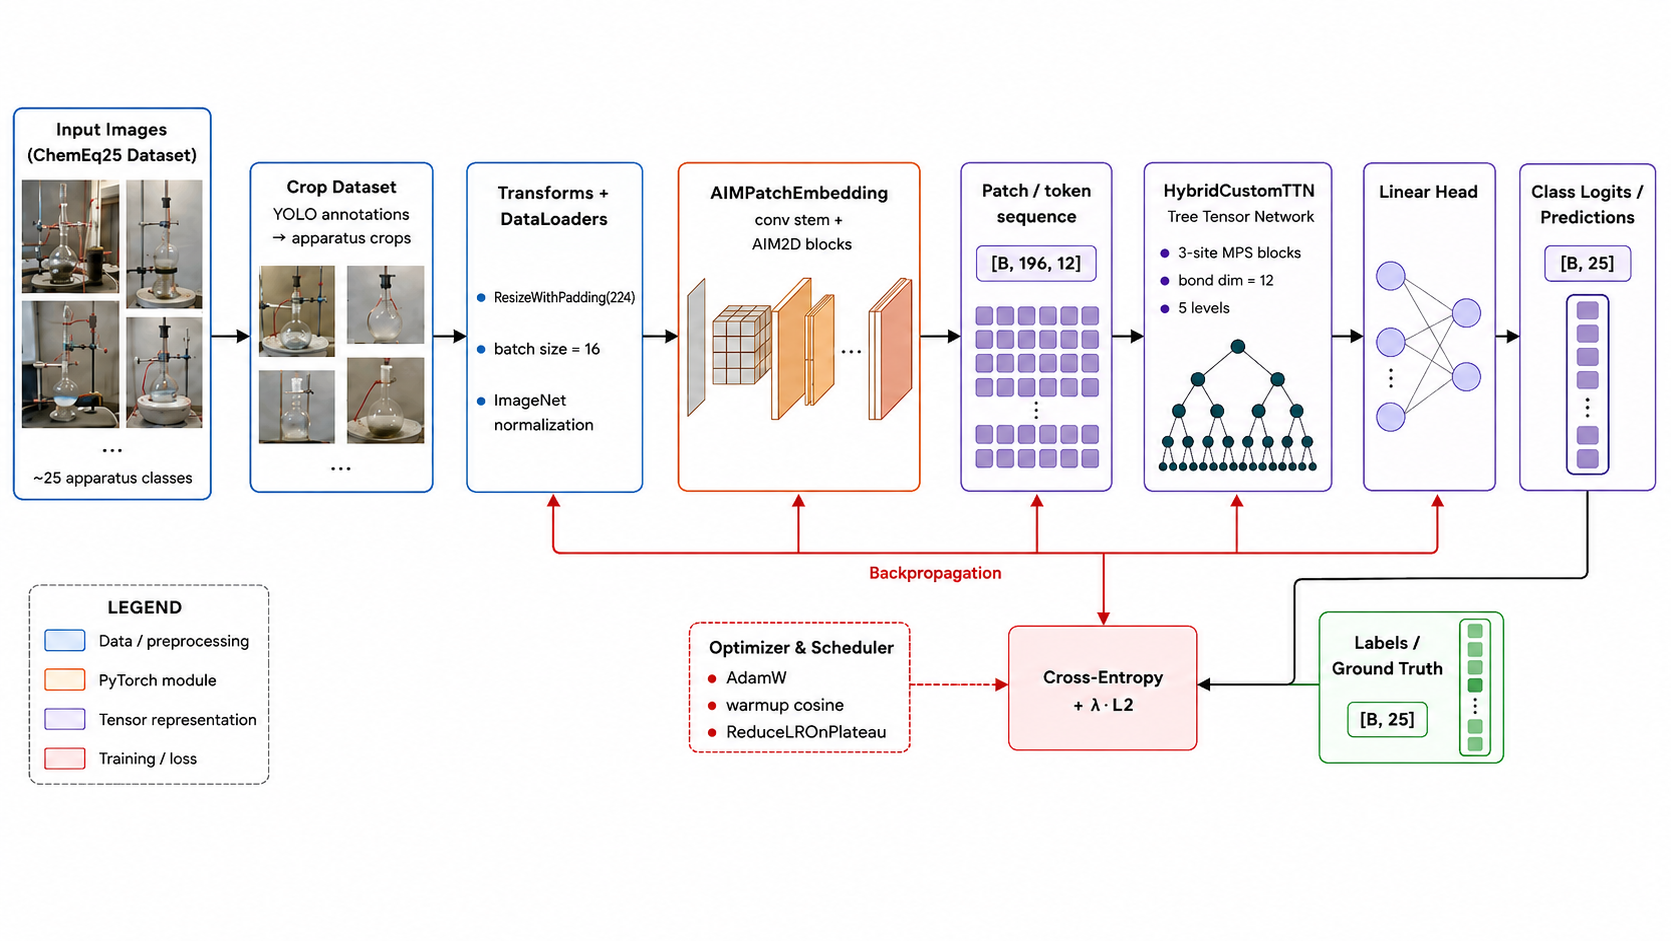
\includegraphics[width=1.0\linewidth]{figures/Pipeline_Scheme.png}
    \caption[Esquema general del pipeline]{Esquema general del pipeline desarrollado en el trabajo. A partir de las imágenes originales y sus anotaciones se generan recortes individuales de objetos, se aplican transformaciones y se agrupan en lotes. Cada imagen procesada entra en la etapa de \textit{embedding}, que produce una secuencia compatible con la red tensorial. La salida de la red tensorial pasa por una cabeza de clasificación y se compara con la etiqueta real mediante la función de pérdida. Las flechas inferiores representan la actualización de parámetros por retropropagación.}
    \label{fig:pipeline_scheme}
\end{figure}

El código del proyecto se organizó de forma modular, separando responsabilidades en distintos módulos diferenciados. Esta organización hace que el proyecto sea mucho más manejable y permite modificar una parte sin alterar el resto. El detalle de la estructura de carpetas se recoge en los anexos.

Por último, cada configuración de los experimentos queda definida por un archivo de configuración en formato YAML (\textit{Yet Another Markup Language}), que fija todos los parámetros relevantes, como el conjunto de datos, el tamaño de imagen, el tipo de \textit{embedding}, la dimensión local y la dimensión de enlace, el número de épocas, el ritmo de aprendizaje, la regularización, el \textit{scheduler} y la semilla aleatoria, entre otros. De este modo, un experimento puede repetirse o compararse leyendo simplemente su configuración, sin depender de notas externas. Esta forma de trabajar es la base de la trazabilidad del proyecto.

\section{Preparación del dataset ChemEq25}

El dataset utilizado en este proyecto es ChemEq25, también llamado en el código \textit{Chemistry Lab Apparatus} \citebox{hossain2025chemistrylabdataset}. Este dataset contiene imágenes de material de laboratorio y anotaciones asociadas a los objetos presentes en cada imagen.

El problema no se trató como una clasificación directa de imágenes completas debido a que, en muchas imágenes aparece más de un objeto, y esos objetos pueden pertenecer a clases distintas. Si se introdujera la imagen completa en el clasificador, la etiqueta sería ambigua. Por eso se reformuló el problema como clasificación por instancia, en el que cada anotación YOLO (\textit{You Only Look Once}) genera un recorte o \textit{crop} de un único objeto, y ese crop se asocia a una clase.

Tras convertir las anotaciones en muestras individuales, los tamaños de los splits fueron:

\begin{center}
\begin{tabular}{c|c}
\textbf{Split} & \textbf{Número de crops} \\
\hline
Entrenamiento & 4863 \\
Validación & 1393 \\
Test & 704 \\
\end{tabular}
\end{center}

El procedimiento de lectura e interpretación (\textit{parser} en inglés) de las anotaciones tuvo que contemplar dos casos. Algunas etiquetas seguían el formato YOLO habitual:

\begin{center}
\texttt{class\_id x\_center y\_center width height}
\end{center}

pero otras contenían más coordenadas, correspondientes a polígonos de segmentación. Para que todo pudiera tratarse de manera uniforme, las anotaciones de cinco coordenadas se interpretaron como cajas YOLO y las anotaciones con más coordenadas se transformaron en la caja rectangular envolvente del polígono.

Después de obtener el \textit{crop}, todas las imágenes deben convertirse a un tamaño común para entrar al modelo. Inicialmente se podía usar un \texttt{Resize(224, 224)} directo, pero esto deforma objetos alargados como pipetas, tubos de ensayo o varillas. Por esa razón se implementó una opción para preservar la relación de aspecto y rellenar hasta obtener una imagen cuadrada. El color de relleno se escogió cercano a la media de \textit{ImageNet}, de forma que tras la normalización el relleno (\textit{padding}) no quedara como un borde artificial demasiado dominante.

\section{Transformaciones y aumento de datos}

El preprocesamiento de las imágenes se separó entre entrenamiento y evaluación. La parte de evaluación consta de un proceso de validación y otro de test. En esta parte no se aplican transformaciones aleatorias, porque se quiere medir el comportamiento del modelo sobre datos estables. En el entrenamiento sí se usa \textit{data augmentation}, con el objetivo de que el modelo no memorice una única apariencia de cada objeto.

Este proceso de aumento de datos se hizo configurable, es decir, que el usuario puede decidir si quiere aplicarlo o no. En ChemEq se usaron opciones como:

\begin{itemize}
    \item \texttt{augmentation\_name = none}, sin aumentos aleatorios.
    \item \texttt{augmentation\_name = basic}, con transformaciones suaves ya existentes.
    \item \texttt{augmentation\_name = light}, añadiendo rotaciones pequeñas y \texttt{RandomErasing} bajo.
\end{itemize}

La configuración final más relevante usó la configuración \texttt{light}, rotaciones de 7 grados y \texttt{RandomErasing} con probabilidad 0,10. La idea fue introducir variabilidad sin destruir la geometría del objeto, porque en material de laboratorio la forma es precisamente una parte importante de la clase.

\section{Representación de la imagen como secuencia}

Una red tensorial no procesa directamente una imagen con forma \texttt{[C, H, W]} (canales, alto y ancho). Su entrada natural es una secuencia ordenada de vectores locales. Dicho de otra forma, son un conjunto de posiciones de entrada en el que cada posición aporta un vector de dimensión fija. Por eso, antes de la red tensorial es necesaria una etapa que transforme la imagen en esa secuencia:

\begin{center}
\texttt{[B, C, H, W] -> [B, L, local\_dim]}
\end{center}

donde \texttt{B} es el número de imágenes que se procesan a la vez (un \textit{batch} o lote), \texttt{L} es el número de posiciones de entrada de la red tensorial y \texttt{local\_dim} es la dimensión del vector asociado a cada posición. Esta etapa se denomina \textit{embedding} de la imagen y es una parte muy importante del modelo, ya que condiciona su rendimiento de manera considerable, porque determina qué información espacial llega a la red tensorial y en qué forma se le entrega.

El primer enfoque que se probó dividía la imagen en cuadrados y proyectaba cada uno de forma independiente con una transformación lineal. Este enfoque resultó insuficiente, ya que al construir la secuencia se pierde la estructura bidimensional de la imagen y la relación de vecindad entre cuadrados contiguos. Por ese motivo, la versión final del proyecto utiliza un \textit{embedding} que conserva la estructura espacial hasta el último momento, denominado en el código \texttt{AIMPatchEmbedding}. A continuación se describe su funcionamiento.

El \texttt{AIMPatchEmbedding} no trocea la imagen, sino que la procesa como un mapa bidimensional que se va reduciendo de tamaño progresivamente. Solo en el último paso ese mapa se aplana para formar la secuencia que recibe la red tensorial. El flujo completo de dimensiones, para imágenes de entrada de $224\times224$, es:

\begin{center}
\texttt{[B, 3, 224, 224]} \\
\texttt{-> stem convolucional -> [B, C\_aim, 14, 14]} \\
\texttt{-> bloques AIM -> [B, C\_aim, 14, 14]} \\
\texttt{-> convolución 1x1 -> [B, local\_dim, 14, 14]} \\
\texttt{-> aplanado + zigzag -> [B, 196, local\_dim]}
\end{center}

La imagen pasa primero por un bloque convolucional inicial, denominado habitualmente \textit{stem}, cuya función es extraer características locales básicas y reducir la resolución espacial de la entrada. Después por una serie de bloques AIM que mantienen el mapa espacial e introducen interacciones entre canales y posiciones, y finalmente por una proyección que ajusta el número de canales a la dimensión local que espera la red tensorial. El mapa resultante de $14\times14$ se aplana en una secuencia de $196$ posiciones de entrada.

El \textit{stem} es la etapa inicial que sustituye el corte en cuadrados por una pequeña red convolucional. Una convolución es una operación que desliza un filtro pequeño sobre la imagen para detectar patrones locales (bordes, texturas, formas) reutilizando los mismos pesos en todas las posiciones. El \textit{stem} se construye como una pila de bloques, cada uno formado por una convolución con paso (\textit{stride}) dos, seguida de una normalización por lotes (\textit{BatchNorm}, que reescala las activaciones usando estadísticas del propio \textit{batch} para estabilizar el entrenamiento) y una función de activación ReLU (que anula los valores negativos e introduce no linealidad).

El paso dos significa que el filtro se desplaza de dos en dos píxeles, de modo que cada bloque reduce a la mitad el alto y el ancho del mapa. El número de bloques viene dado por el hiperparámetro \texttt{patch\_size}, que en este \textit{embedding} ya no representa el tamaño de un cuadrado, sino el factor total de reducción espacial. Debe ser una potencia de dos, y el número de bloques es $\log_2(\texttt{patch\_size})$. Con \texttt{patch\_size = 16} se encadenan cuatro bloques, que reducen la imagen de la siguiente forma:

\begin{center}
\texttt{224 -> 112 -> 56 -> 28 -> 14}
\end{center}

El primer bloque transforma los tres canales de color en \texttt{aim\_channels} canales, y los siguientes mantienen ese número. El resultado es un mapa \texttt{[B, aim\_channels, 14, 14]} en el que cada una de las $14\times14$ posiciones del mapa pasará a ser una posición de entrada de la red tensorial.

Sobre el mapa producido por el \textit{stem} se aplican uno o varios bloques AIM, inspirados en el trabajo \textit{Deep Tree Tensor Networks for Image Recognition} \citebox{nie2025deeptreetensornetworks}. Cada bloque recibe un mapa \texttt{[B, C, H, W]} y devuelve otro de la misma forma, lo que permite encadenar varios y, como se verá, añadir una conexión residual.

La idea central del bloque es construir dos ramas que aplican las mismas dos familias de operaciones, pero en orden inverso:

\begin{itemize}
    \item \textbf{Rama 1:} primero una transformación lineal que mezcla los canales en cada píxel y una convolución que aplica un filtro espacial independiente a cada canal sin mezclar información entre canales.
    \item \textbf{Rama 2:} primero una convolución agrupada (\textit{grouped}), que procesa cada canal de entrada por separado para generar varios canales nuevos, y después una transformación lineal que mezcla los canales.
\end{itemize}

Internamente ambas ramas expanden el número de canales por un factor configurable (\texttt{expansion\_ratio}), lo que da al bloque más capacidad de representación antes de volver a comprimir. Las salidas de las dos ramas se combinan mediante un producto de Hadamard, esto es, una multiplicación elemento a elemento de dos tensores de la misma forma:

\begin{center}
\texttt{interaction = f1(x) * f2(x)}
\end{center}

Este producto es la clave del bloque y el motivo por el que encaja bien delante de una red tensorial. Las dos ramas se construyen sin término independiente (\textit{bias}) y sin funciones de activación intermedias, de modo que cada una es una transformación lineal de la entrada. Al multiplicarlas elemento a elemento, el resultado es bilineal, es decir, cuadrático en la entrada. Se introduce así una interacción multiplicativa entre las características de la imagen, justo el tipo de operación que las redes tensoriales expresan de forma natural, y sin recurrir a no linealidades del tipo ReLU o sigmoide. El nombre del módulo en la literatura, \textit{Antisymmetric Interaction Module} (AIM), alude precisamente a esa construcción en orden inverso de las dos ramas antes del producto.

Tras el producto, el resultado se normaliza con una normalización por capas (\textit{LayerNorm}, que reescala cada vector de canales para estabilizar su escala y distribución) y se proyecta de vuelta al número original de canales mediante una convolución $1\times1$, de manera que la salida pueda sumarse con la entrada del bloque. Esta suma es una conexión residual; en lugar de reemplazar la entrada, el bloque aprende una corrección que se le añade,

\begin{center}
\texttt{salida = x + s * correccion}
\end{center}

donde \texttt{s} es un factor de escala entrenable inicializado a un valor pequeño. Inicializarlo pequeño hace que, al comienzo del entrenamiento, el bloque se comporte casi como la identidad y no desestabilice las activaciones que recibirá la red tensorial. La etapa AIM aplica \texttt{num\_aim\_blocks} bloques de este tipo de forma consecutiva.

Después de los bloques AIM, una última convolución $1\times1$ ajusta el número de canales desde \texttt{aim\_channels} hasta \texttt{local\_dim}, la dimensión que espera la red tensorial en cada posición. El mapa resultante, de forma \texttt{[B, local\_dim, 14, 14]}, se reordena para situar los canales al final y se aplana convirtiendo la rejilla espacial en una secuencia:

\begin{center}
\texttt{[B, local\_dim, 14, 14] -> [B, 196, local\_dim]}
\end{center}

El orden en que se recorren las $196$ posiciones no es indiferente. Un recorrido por filas (\textit{row-major}) saltaría del final de una fila al principio de la siguiente, introduciendo una discontinuidad espacial entre posiciones consecutivas de la secuencia. Para suavizar este efecto se emplea un recorrido en zigzag. Las filas pares se recorren de izquierda a derecha y las impares de derecha a izquierda, de modo que dos posiciones contiguas en la secuencia tienden a ser también vecinas en la imagen. Cada una de las $196$ posiciones resultantes es un vector local de dimensión \texttt{local\_dim} y constituye una posición de entrada de la red tensorial descrita en la siguiente sección.

\medskip

En conjunto, este \textit{embedding} conserva la estructura espacial bidimensional de la imagen hasta el momento mismo del aplanado, en lugar de destruirla al inicio. Las convoluciones, al compartir pesos entre posiciones, actúan como un sesgo inductivo y como una forma de regularización, y la interacción multiplicativa del bloque AIM aporta una no linealidad coherente con el lenguaje de las redes tensoriales. La conexión residual, por su parte, permite que la etapa inicial parta de un comportamiento próximo a la identidad y estabilice el entrenamiento del modelo completo.

\section{Arquitectura tensorial propuesta}\label{sec:arquitectura}

La secuencia de $196$ vectores locales producida por el \textit{embedding} es la entrada de la red tensorial entrenable, que procesa la información hasta obtener un único vector con el que se decide la clase. El tipo de red tensorial es una jerárquica de tipo \textit{Tree Tensor Network} (TTN), denominada en el código \texttt{HybridCustomTTN}, que se describe a continuación.

La idea de una TTN es organizar el cálculo como un árbol. Las posiciones de entrada se agrupan de tres en tres, cada grupo se contrae con un pequeño bloque tensorial que produce un solo vector de salida, y ese vector pasa a ser una entrada del siguiente nivel del árbol. El proceso se repite, reduciendo el número de posiciones en cada nivel, hasta llegar a un único vector raíz que resume toda la imagen. Que los grupos sean de tres elementos es lo que se denomina aridad tres del árbol.

\begin{figure}[H]
    \centering
    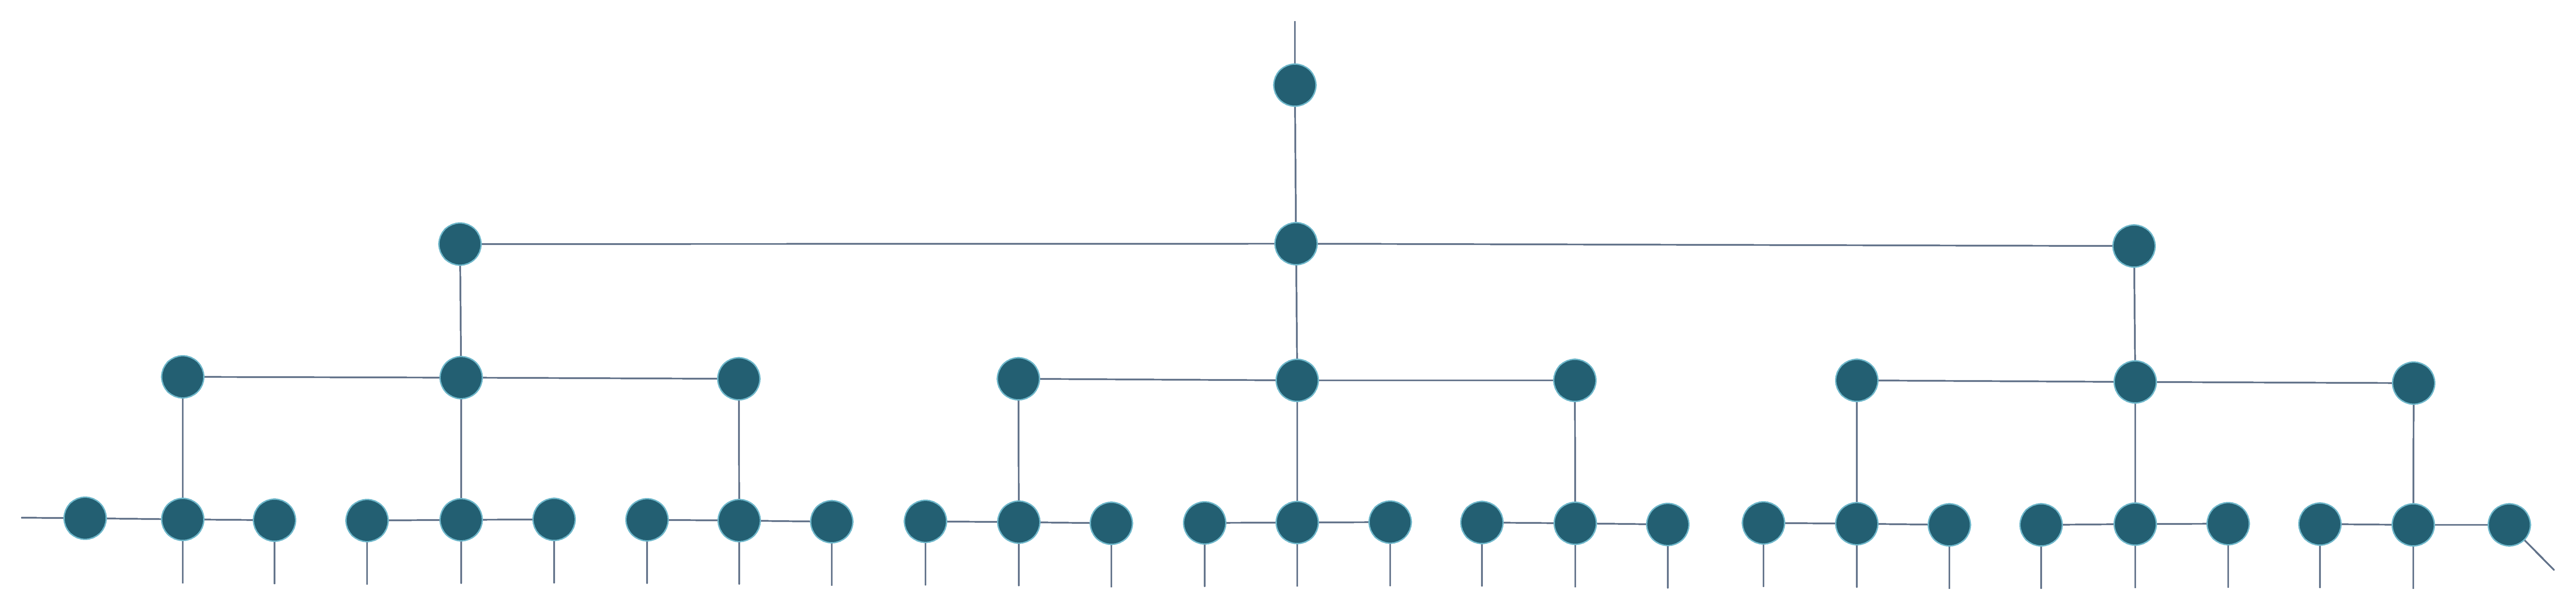
\includegraphics[width=1\linewidth]{figures/ttn_model.pdf}
    \caption[Diagrama de la \textit{Tree Tensor Network} propuesta]{Diagrama de la TTN. Es una imagen orientativa, ya que representa tres niveles cuando la arquitectura empleada tiene cinco. Las posiciones de entrada se agrupan de tres en tres y se contraen jerárquicamente hasta un único vector raíz. Imagen de elaboración propia con la librería Tensor-Network-Editor, creada por Alejandro Mata Ali. \citebox{Mata_Ali_Tensor_Network_Editor_2026}}
    \label{fig:ttn_diagram}
\end{figure}

En el lenguaje de redes tensoriales conviene distinguir dos tipos de índices. Los índices físicos (o de entrada) son los que conectan la red con los datos; por cada posición de entrada hay un índice físico cuya dimensión es la del vector local que llega a esa posición. En el primer nivel esa dimensión es \texttt{local\_dim}, la que produce el \textit{embedding}. Los índices virtuales (o de enlace) son internos; conectan unos tensores con otros dentro de la red y no tocan los datos. Su dimensión común se denomina dimensión de enlace (\texttt{bond\_dim}).

La dimensión de enlace es el principal parámetro que controla la capacidad del modelo. Cuanto mayor es \texttt{bond\_dim}, más información puede transmitirse a través de cada conexión interna y más ricas son las correlaciones que la red puede representar entre distintas partes de la imagen, a costa de más parámetros y más coste de cálculo. Junto con la topología del árbol, es la decisión de diseño que regula el equilibrio entre capacidad y eficiencia.

La unidad básica de la TTN es un bloque tensorial de tres nodos, con la estructura de una MPS corta. Cada bloque está formado por un nodo izquierdo, uno central y uno derecho. El nodo izquierdo tiene un índice físico de entrada y un índice virtual que lo une al central. El nodo central tiene un índice físico de entrada, dos índices virtuales (uno hacia el nodo izquierdo y otro hacia el derecho) y un índice de salida. El nodo derecho tiene un índice físico de entrada y un índice virtual que lo une al central.

El índice de salida se sitúa en el nodo central y tiene dimensión \texttt{bond\_dim}; es el que conecta el bloque con el nivel superior del árbol. Cada bloque recibe tres vectores de entrada (uno por nodo) y los contrae junto con sus tres tensores para producir un único vector de salida. Si se denota por $v^{(1)}, v^{(2)}, v^{(3)}$ a los tres vectores de entrada, por $A$, $C$ y $B$ a los tensores de los nodos izquierdo, central y derecho, y se usan las letras $a,b$ para los índices virtuales, $i,j,k$ para los físicos y $\beta$ para el de salida, la salida del bloque es:

\begin{equation}
o_{\beta} \;=\; \sum_{a,b}\;\sum_{i,j,k} A_{a\,i}\, C_{a\,b\,j\,\beta}\, B_{b\,k}\; v^{(1)}_{i}\, v^{(2)}_{j}\, v^{(3)}_{k}.
\end{equation}

Los índices virtuales $a$ y $b$ tienen dimensión \texttt{bond\_dim}, los físicos $i,j,k$ tienen la dimensión de entrada del nivel y el índice de salida $\beta$ tiene de nuevo dimensión \texttt{bond\_dim}. La contracción combina de forma multiplicativa la información de los tres vectores de entrada, lo que conecta directamente con la motivación de usar redes tensoriales. La salida depende de productos entre las componentes de la entrada, no solo de sumas ponderadas.

Los tres tensores de cada bloque son parámetros entrenables del modelo. En la implementación esto exigió declararlos de un tipo específico de TensorKrowch (\texttt{ParamNode}), de modo que sus valores se registran como parámetros del modelo y reciben gradientes durante el entrenamiento; si se hubieran creado como nodos ordinarios, no aparecerían como parámetros entrenables. Sus valores se inicializan con ruido aleatorio de desviación típica pequeña ($0{,}02$), un valor que mantiene las contracciones numéricamente estables a medida que se asciende por los niveles del árbol.

El número de posiciones de un nivel no siempre es múltiplo de tres. Cuando el último grupo queda incompleto, las posiciones que faltan se rellenan con nodos constantes, no entrenables, cuyo vector es $[1, 0, \dots, 0]$. Estos nodos de relleno (\textit{padding}) completan el grupo para que el bloque pueda contraerse, pero no aportan parámetros ni introducen información, ya que su vector es fijo y neutro. De esta forma la estructura jerárquica se mantiene regular sin distorsionar el aprendizaje.

Cada nivel del árbol se implementó como una red tensorial independiente (\texttt{TTNLevel}) que contrae únicamente su propio nivel de bloques de tres nodos y devuelve un tensor de PyTorch ordinario. El enlace entre un nivel y el siguiente no se hace dentro de TensorKrowch, sino en PyTorch: la salida de un nivel, antes de entrar en el siguiente, pasa por una pequeña transformación estándar formada por una normalización por capas (\textit{LayerNorm}), una capa lineal y una activación ReLU:

\begin{center}
\texttt{nivel -> LayerNorm -> Linear -> ReLU -> nivel siguiente}
\end{center}

Esta combinación es la razón del nombre \texttt{HybridCustomTTN}. Es híbrida porque las contracciones tensoriales se realizan con TensorKrowch, mientras que las transformaciones intermedias, el entrenamiento y la integración del modelo se gestionan con PyTorch. Las transformaciones entre niveles aportan flexibilidad adicional y ayudan a estabilizar las escalas de los vectores al pasar de un nivel a otro.

Partiendo de las $196$ posiciones de entrada y agrupando de tres en tres, el número de posiciones se reduce nivel a nivel de la forma

\begin{center}
\texttt{196 -> 66 -> 22 -> 8 -> 3 -> 1},
\end{center}

de modo que la arquitectura empleada consta de cinco niveles tensoriales y cuatro transformaciones intermedias. La salida del último nivel es un único vector raíz de dimensión \texttt{bond\_dim} que condensa la información de toda la imagen.

El vector raíz no es todavía una predicción. Para obtener una puntuación por clase se aplica una cabeza de clasificación, que en su versión más sencilla es una única capa lineal que transforma el vector raíz de dimensión \texttt{bond\_dim} en un vector de dimensión igual al número de clases ($25$ en ChemEq25). Las componentes de ese vector son las puntuaciones sin normalizar de cada clase (\textit{logits}), que en la etapa de entrenamiento se compararán con la etiqueta real mediante la función de pérdida descrita más adelante. Opcionalmente, esta cabeza puede sustituirse por un pequeño perceptrón multicapa con una capa oculta, una activación y regularización por \textit{dropout}, aunque la versión lineal es la que define el modelo de referencia.

\section{Entrenamiento y regularización}\label{sec:entrenamiento}

Una vez definidos el \textit{embedding} y la red tensorial, el modelo se entrena ajustando sus parámetros para que clasifique correctamente los recortes. En cada paso, el modelo procesa un \textit{batch} de imágenes y produce sus puntuaciones por clase; una función de pérdida mide cuánto se equivoca, y a partir de ese error se calculan los gradientes que indican cómo modificar cada parámetro para reducirlo. Esta sección explica las decisiones tomadas en ese proceso: la función de pérdida, las técnicas de regularización y el control del ritmo de aprendizaje.

Para entrenar el clasificador se empleó la entropía cruzada, una función de pérdida habitual en problemas de clasificación con varias clases. El modelo no devuelve directamente probabilidades, sino una puntuación para cada clase (los \textit{logits} introducidos antes). Durante el cálculo de la pérdida, esas puntuaciones se transforman internamente en probabilidades normalizadas y se penaliza al modelo cuando asigna una probabilidad baja a la clase correcta. Cuanto más confiado está el modelo en la clase verdadera, menor es la pérdida.

En la implementación, esta función (\texttt{CrossEntropyLoss} en PyTorch) combina internamente la normalización en probabilidades (\textit{softmax}) y la comparación con la etiqueta correcta. Por eso el modelo no necesita aplicar esa normalización en su capa de salida, basta con que produzca los \textit{logits}. Esta combinación interna evita duplicar operaciones y hace el entrenamiento numéricamente más estable.

Durante el entrenamiento se aplicó además un suavizado de etiquetas (\textit{label smoothing}). En lugar de exigir al modelo que asigne toda la probabilidad a la clase correcta y exactamente cero al resto, el objetivo se relaja ligeramente, dejando una pequeña parte de probabilidad repartida entre las demás clases. Esto evita que el modelo se vuelva excesivamente confiado y suele mejorar su capacidad de generalizar a imágenes nuevas.

El suavizado solo se usa en entrenamiento. En la evaluación se emplea la entropía cruzada normal, sin suavizado, de modo que la pérdida de validación (\texttt{eval\_loss}) sigue midiendo el ajuste real del modelo frente a las etiquetas verdaderas y permite comparar experimentos de forma coherente.

El optimizador es el algoritmo que decide cómo actualizar los parámetros del modelo a partir de los gradientes. Se utilizó AdamW (\texttt{AdamW}), una variante muy extendida del optimizador Adam. Adam adapta automáticamente el tamaño del paso de actualización para cada parámetro, usando estimaciones del comportamiento reciente de sus gradientes, lo que suele acelerar y estabilizar el entrenamiento frente a un descenso de gradiente simple. La variante AdamW incorpora además, de forma adecuada, una penalización que tiende a mantener pequeños los pesos del modelo (\textit{weight decay}), descrita a continuación.

La regularización agrupa las técnicas que evitan que el modelo se limite a memorizar las imágenes de entrenamiento (sobreajuste) en lugar de aprender características que generalicen. En este trabajo se combinaron dos mecanismos. El primero es la penalización por reducción de pesos (\textit{weight decay}) que incorpora AdamW, que empuja suavemente los pesos hacia valores pequeños. El segundo es una penalización L2 explícita y configurable. Durante el entrenamiento se añade a la pérdida un término proporcional a la suma de los cuadrados de los pesos del modelo. Esta penalización se aplica solo a las matrices de pesos, excluyendo los términos independientes y los parámetros de las capas de normalización, que no conviene penalizar de la misma forma.

Un detalle importante de trazabilidad es que, aunque este término de regularización se suma a la pérdida que guía la actualización de los parámetros, la métrica registrada como \texttt{train\_loss} conserva únicamente la entropía cruzada. De este modo, la pérdida de entrenamiento y la de validación miden lo mismo y son directamente comparables entre sí y entre experimentos.

El ritmo de aprendizaje (\textit{learning rate}) determina cómo de grandes son los pasos con los que se actualizan los parámetros en cada iteración. Un valor demasiado grande puede hacer que el entrenamiento se vuelva inestable; uno demasiado pequeño lo ralentiza. Para gestionarlo se combinaron dos mecanismos.

El primero es un calentamiento inicial (\textit{warmup}). Durante las primeras épocas, el ritmo de aprendizaje no parte de su valor máximo, sino que crece de forma gradual, ya sea de manera lineal o siguiendo un perfil más suave, hasta alcanzar el valor objetivo. Empezar con pasos pequeños evita las grandes oscilaciones que pueden producirse al inicio, cuando los parámetros aún están lejos de una buena solución.

El segundo mecanismo actúa una vez terminado el calentamiento: el ritmo de aprendizaje se reduce automáticamente cuando la pérdida de validación deja de mejorar durante varias épocas seguidas (\texttt{ReduceLROnPlateau}). La idea es dar pasos más finos a medida que el modelo se acerca a una solución y ya no progresa con el ritmo anterior. La implementación contempla también, como alternativa, un descenso suave y continuo del ritmo de aprendizaje a lo largo del entrenamiento (\textit{cosine decay}).

Finalmente, el estado del optimizador y del controlador del ritmo de aprendizaje se guarda junto con el mejor modelo en cada punto de control (\textit{checkpoint}). Esto permite reanudar un entrenamiento interrumpido exactamente en las mismas condiciones en que se dejó, lo que resultó útil para los entrenamientos largos ejecutados en el servidor.

\section{Métricas, diagnósticos y trazabilidad}

Cada entrenamiento genera una carpeta dentro de \texttt{runs/}. En ella se guardan la configuración resuelta, el checkpoint del mejor modelo, el archivo \texttt{metrics.csv}, las curvas de pérdida y los diagnósticos. Esto fue fundamental para poder reconstruir qué se había probado y con qué parámetros.

En cada época se registran en \texttt{metrics.csv} varias métricas que resumen el comportamiento del modelo sobre el conjunto de entrenamiento y sobre el de validación. La primera es la pérdida (\texttt{train\_loss} y \texttt{eval\_loss}), que mide cómo de lejos queda la predicción de la respuesta correcta. Cuanto más baja es, mejor es el ajuste, y penaliza especialmente los fallos cometidos con mucha seguridad. La versión \texttt{train} se calcula sobre los datos de entrenamiento y la \texttt{eval} sobre los recortes de validación, que el modelo no ha visto durante el ajuste. A continuación está el acierto o \textit{accuracy} top-1 (\texttt{train\_accuracy} y \texttt{eval\_accuracy}), que es la fracción de recortes en los que la clase más probable para el modelo coincide con la real; es la medida más directa de rendimiento, de modo que un valor de 0,96 indica que el modelo acierta la primera predicción en el 96\% de los casos. El acierto top-5 (\texttt{eval\_top5\_accuracy}) es una versión más permisiva; cuenta los recortes en los que la clase correcta está entre las cinco más probables, aunque no sea la primera, y sirve para ver si el modelo se acerca a la respuesta correcta cuando su primera elección falla. Por último, la confianza media en aciertos y en errores (\texttt{mean\_confidence\_correct} y \texttt{mean\_confidence\_wrong}) recoge la probabilidad que el modelo asigna a la clase que elige; al promediarla por separado según acierte o falle, se puede comprobar si está bien calibrado o si se equivoca con demasiada seguridad.

Al terminar cada entrenamiento, a partir del mejor checkpoint se calculan además métricas por clase sobre el conjunto de validación. La precisión (\textit{precision}) de una clase indica, de todos los recortes que el modelo asigna a ella, qué fracción le pertenece realmente, por lo que penaliza los falsos positivos. La exhaustividad (\textit{recall}) indica, de todos los recortes que pertenecen de verdad a esa clase, qué fracción consigue recuperar el modelo, por lo que penaliza los que se le escapan. El F1 combina ambas en su media armónica, que da más peso al menor de los dos valores, de manera que solo es alto cuando la precisión y la exhaustividad lo son a la vez. Para resumir el rendimiento global se usa la media macro de estas tres métricas, es decir, el promedio simple sobre las 25 clases dando el mismo peso a cada una con independencia de cuántos recortes contenga, lo que evita que las clases más numerosas dominen el resultado.

Junto a estas métricas se generan otros diagnósticos, como la matriz de confusión, la distribución de predicciones, las principales confusiones, las curvas \textit{precision-recall} y las curvas F1-confianza. La matriz de confusión es especialmente útil, ya que sus filas representan la clase real y sus columnas la clase predicha, de modo que la diagonal recoge los aciertos y los valores fuera de ella muestran entre qué clases se confunde el modelo. En este TFG todas estas métricas se interpretan como métricas de clasificación de recortes, una distinción importante porque el paper de ChemEq25 evalúa modelos de detección, mientras que aquí el modelo clasifica recortes ya generados a partir de las anotaciones, sin localizar cajas ni medir solapamientos.

\section{Comparación con ResNet50}\label{sec:resnet}

Para situar el rendimiento de la arquitectura tensorial dentro de un marco más amplio, se incorporó como referencia una arquitectura convolucional estándar de visión artificial; ResNet50. El objetivo de esta comparación no es demostrar que un modelo supere al otro, sino contextualizar los resultados de la red tensorial frente a un modelo ampliamente utilizado y bien comprendido, e identificar qué decisiones de diseño influyen más en el rendimiento.

La comparación se diseñó para ser justa, en el sentido de aislar el efecto de la arquitectura. ResNet50 clasifica exactamente los mismos recortes que la red tensorial. Se utilizan las mismas particiones de entrenamiento, validación y test, las mismas $25$ clases de ChemEq25 y la misma normalización de las imágenes (con la media y la desviación típica de ImageNet que ya produce la preparación de datos). Además, ambos modelos comparten el mismo bucle de entrenamiento y evaluación y se valoran con las mismas métricas. De este modo, la principal diferencia controlada entre los experimentos es la arquitectura del modelo.

El modelo se tomó de la librería \texttt{torchvision}, sustituyendo únicamente su capa final de clasificación por una capa lineal hacia las $25$ clases del problema (con la opción de añadir regularización por \textit{dropout}). Sobre esta base se evaluaron dos esquemas de entrenamiento, que se corresponden con dos formas distintas de inicializar los pesos del modelo:

\begin{itemize}
    \item \textbf{Entrenamiento desde cero.} La red parte de pesos aleatorios y aprende únicamente a partir de los recortes de ChemEq25, sin ningún conocimiento previo. Sirve como referencia de cuánto puede aprender la arquitectura con los datos disponibles del problema.

    \item \textbf{Ajuste fino.} La red parte de pesos preentrenados sobre ImageNet, un gran conjunto de imágenes de uso general, y todos sus pesos se actualizan durante el entrenamiento, ajustando las características visuales generales aprendidas previamente al problema concreto de material de laboratorio. Constituye la referencia más habitual y fuerte de visión artificial.
\end{itemize}

En la implementación, ambos esquemas se controlan con una opción de configuración que indica si se parte de pesos preentrenados sobre ImageNet o de pesos aleatorios. Cada esquema se entrenó con una tasa de aprendizaje distinta según su inicialización. Para el modelo entrenado desde cero se empleó un valor mayor, mientras que para el modelo preentrenado se utilizó un valor menor durante el ajuste fino, con el objetivo de adaptar sus pesos al nuevo problema sin modificar bruscamente las características ya aprendidas. Estos experimentos de referencia incorporaron además un criterio de parada temprana (\textit{early stopping}), que detiene el entrenamiento cuando la pérdida de validación deja de mejorar durante un número fijo de épocas, evitando épocas innecesarias una vez alcanzado el mejor rendimiento. Los resultados cuantitativos de cada esquema, junto con su comparación con la red tensorial propuesta, se presentan y discuten en el capítulo de resultados.

\section{Reproducibilidad y ejecución en servidor}\label{sec:reproducibilidad}

Todos los entrenamientos se ejecutaron en los servidores Lorca de la universidad. El uso de estos recursos forma parte de la metodología del proyecto, porque permitió lanzar experimentos largos, aprovechar la aceleración por GPU, guardar puntos de control y analizar las métricas con posterioridad.

\begin{figure}[H]
    \centering
    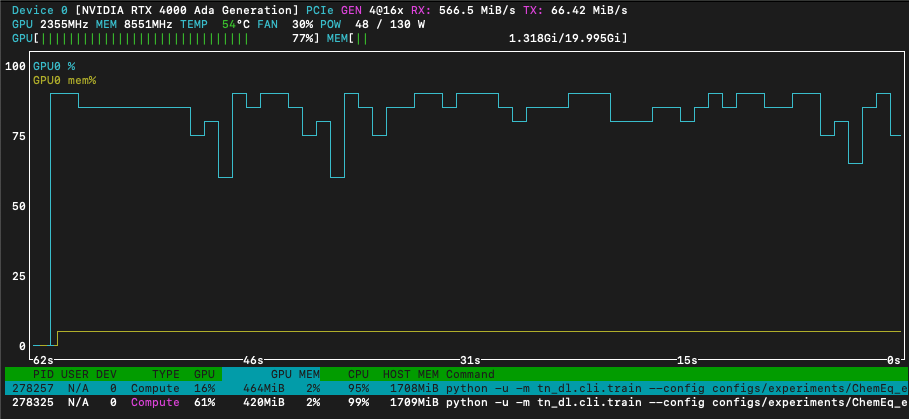
\includegraphics[width=1.0\linewidth]{figures/GPU_picture.png}
    \caption{Captura de una GPU NVIDIA RTX 4000 Ada Generation del servidor Lorca de la UEM ejecutando dos procesos de entrenamiento en paralelo.}
    \label{fig:gpu_lorca}
\end{figure}

El trabajo en el servidor obligó a cuidar el entorno de Python, las dependencias y los scripts de lanzamiento, así como a registrar de forma ordenada los resultados de cada ejecución. Esto fue especialmente importante porque muchas pruebas se lanzaron en paralelo o en días distintos; sin un registro fiable habría sido difícil distinguir si una mejora provenía de la arquitectura, del preprocesamiento, de la semilla aleatoria, del ritmo de aprendizaje o de la regularización.

La reproducibilidad se cuidó de forma explícita. Cada ejecución fija una semilla aleatoria, lo que hace que el entrenamiento sea repetible, y conserva la configuración resuelta y las métricas ya descritas, de modo que un experimento puede reconstruirse a partir de esos archivos sin depender de notas externas. El código completo del proyecto está disponible en un repositorio público enlazado en los anexos, donde se incluye también una nota con las instrucciones necesarias para reproducir los experimentos.

\chapter{RESULTADOS}\label{sec:Resultados}

En este capítulo se exponen los resultados que se han ido obteniendo a lo largo del proyecto. La idea es ir reconstruyendo el camino experimental que llevó a obtener los resultados finales. Se explicará qué ideas se probaron primero, qué problemas surgieron, qué hipótesis aparecieron a partir de los datos y qué cambios fueron mejorando el modelo.

Hay una aclaración importante antes de empezar. El paper de ChemEq25 compara modelos de detección como \textit{YOLOv11} o \textit{RF-DETR} \citebox{hossain2025chemistrylabdataset}. En este TFG el planteamiento final no es detección, sino clasificación de crops generados a partir de las anotaciones YOLO. Por tanto, las métricas como \textit{accuracy}, F1 o \texttt{classification\_mAP} sirven para evaluar nuestro clasificador, pero no son directamente equivalentes al \textit{mAP@50} de un detector. Aun así, sí permiten demostrar que un modelo de \textit{deep learning} basado en TN puede funcionar de forma competitiva en un problema de clasificación de imágenes.

\section{Primeros experimentos con Flowers102}

Flowers102 fue el dataset de prueba inicial. No era el objetivo final del TFG, pero sirvió para comprobar que el pipeline entrenaba, que las métricas se guardaban bien y que la red tensorial recibía gradientes. Además, al tener 102 clases, era un buen primer dataset de prueba para detectar si el modelo estaba aprendiendo algo o si se quedaba cerca del azar.

\subsection{Modelo original CustomTTN}

Con el modelo original \texttt{CustomTTN} se hicieron los primeros experimentos. Los resultados fueron los siguientes:

\begin{figure}[H]
    \centering
    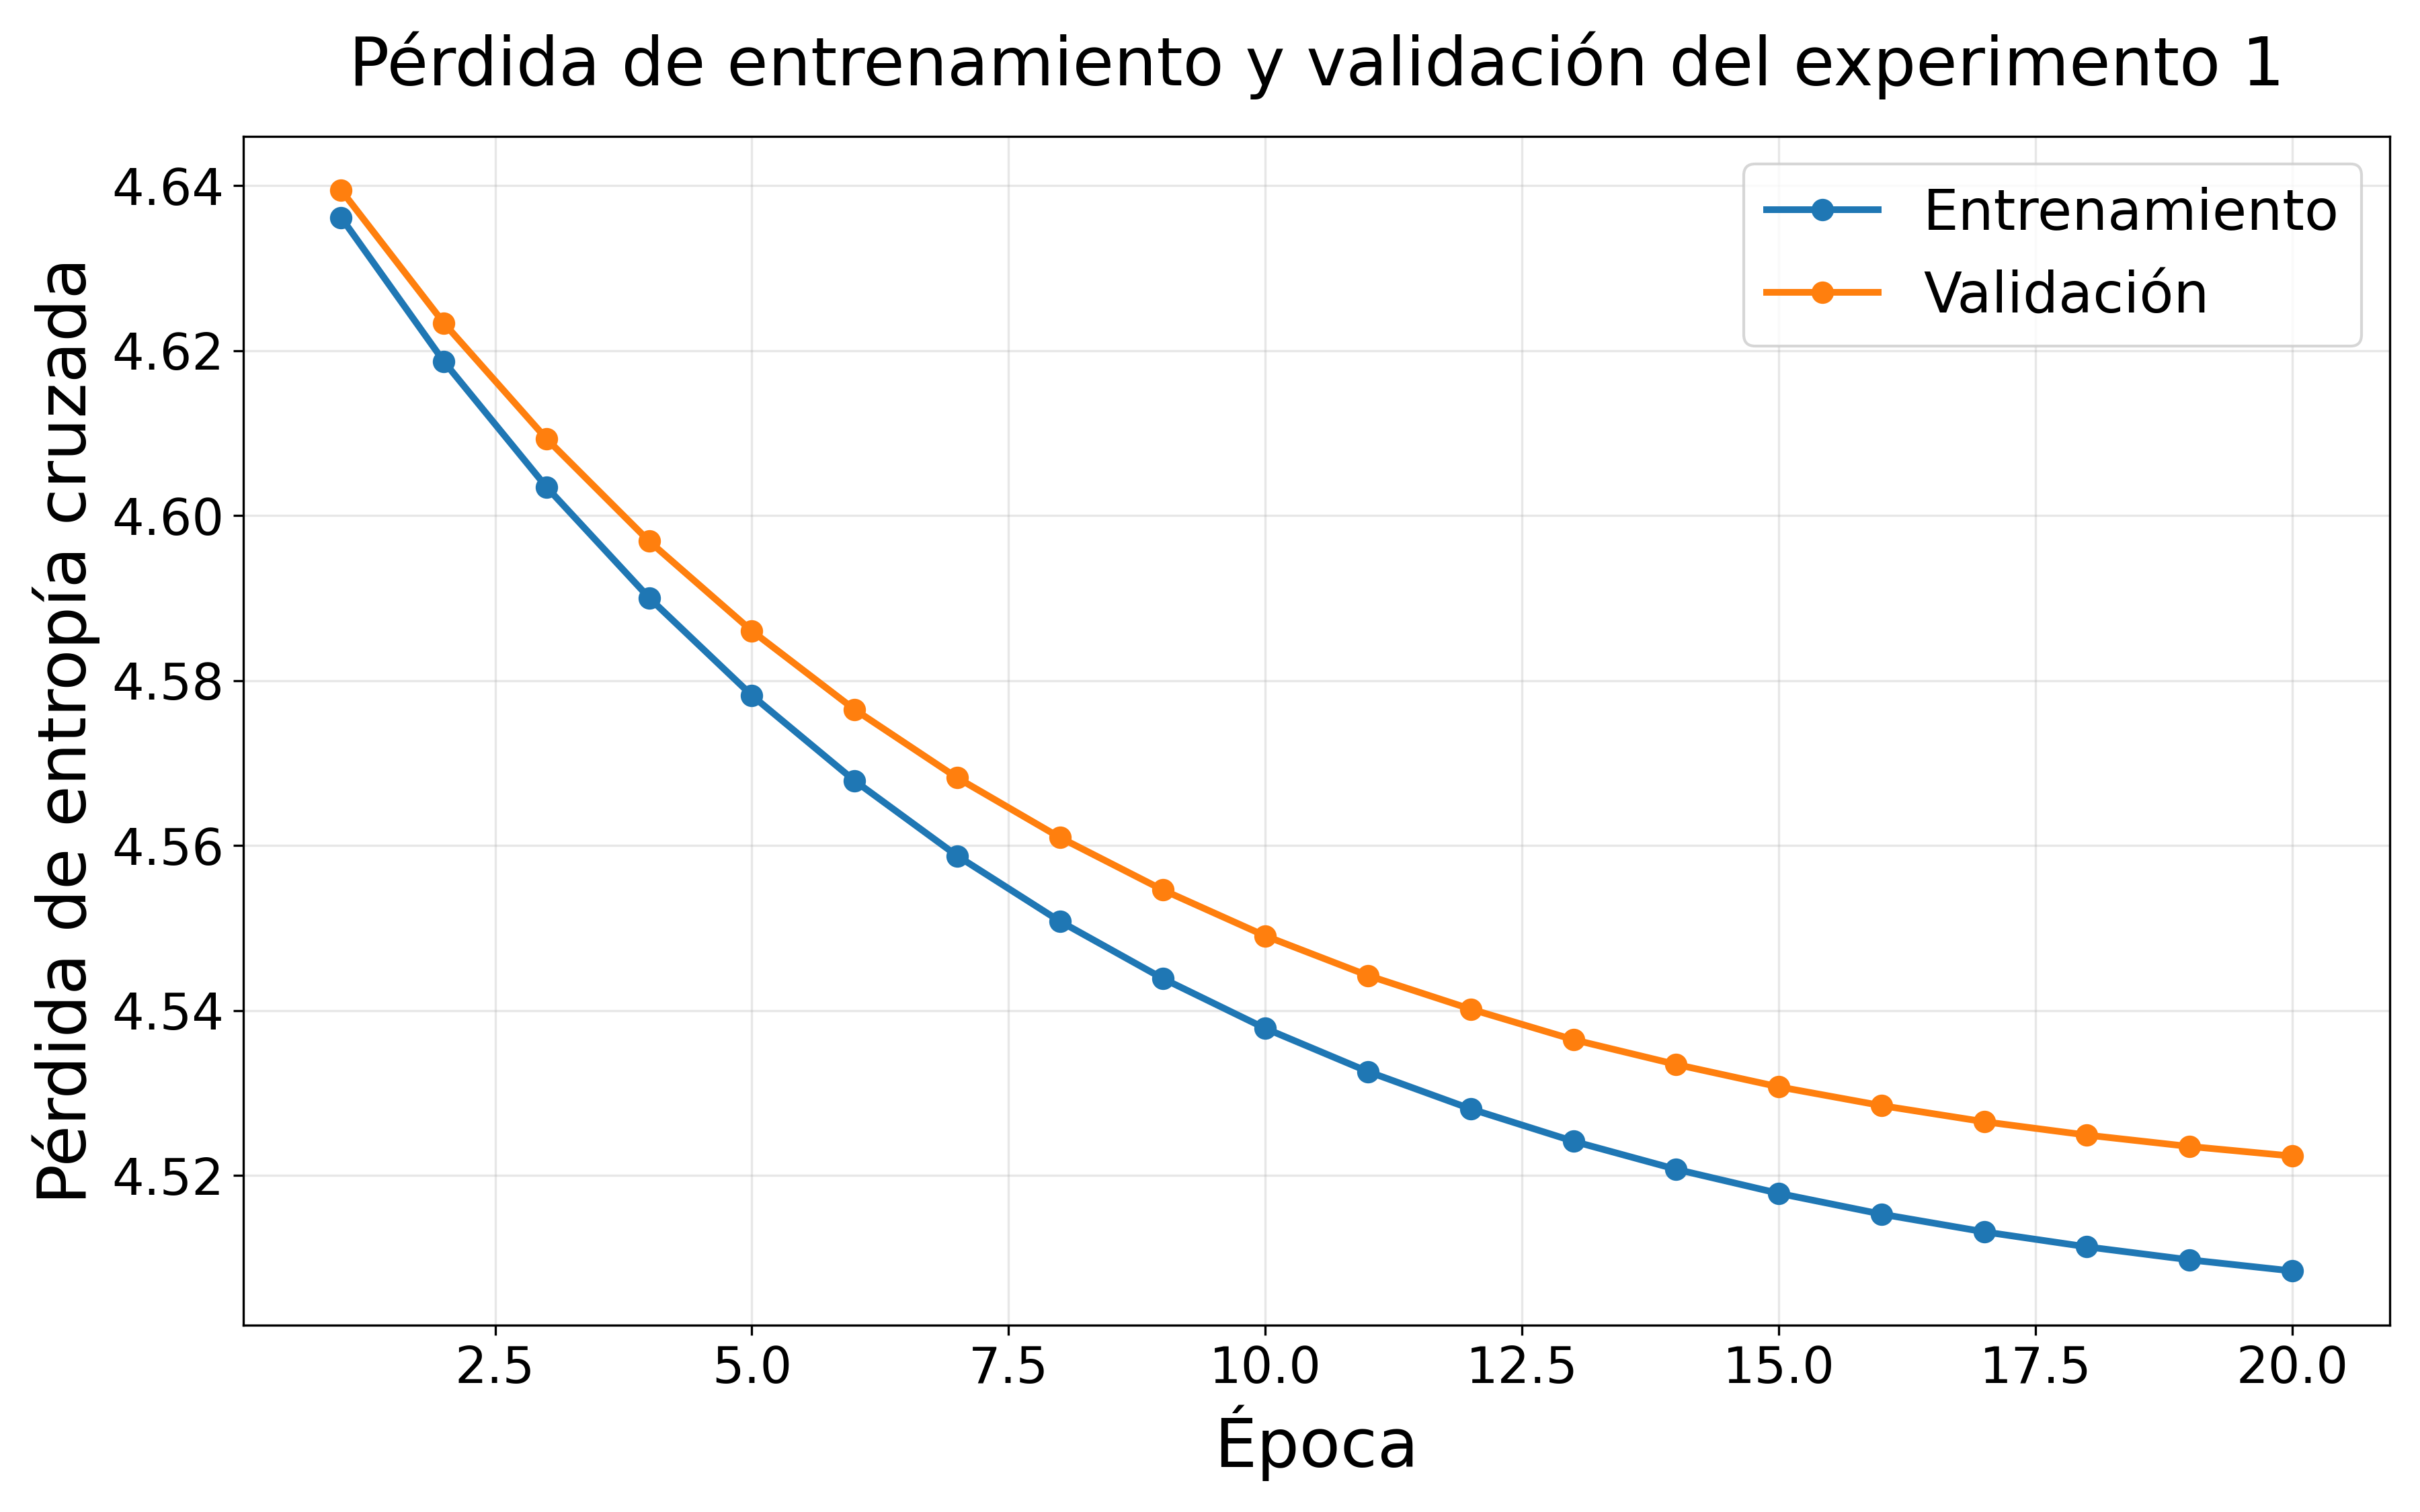
\includegraphics[width=0.55\linewidth]{figures/Experiments_logs/loss_curve_04-21.png}
    \caption{Curvas de pérdida del primer experimento con \texttt{CustomTTN} sobre Flowers102.}
    \label{fig:loss_curve_04-20}
\end{figure}

\begin{table}[H]
\centering
\small
\begin{tabular}{lcccc}
\toprule
\textbf{Experimento} & \textbf{Mejor acc. eval} & \textbf{Época} & \textbf{Mejor eval loss} & \textbf{Eval loss final} \\
\midrule
\texttt{1} & 3,58\% & 9 & 4,5153 & 4,5156 \\
\bottomrule
\end{tabular}
\caption{Resumen representativo del primer experimento con \texttt{CustomTTN}.}
\label{tab:customttn_inicial}
\end{table}

En este momento se estaba usando Flowers102. Si calculamos $\ln(102)$ se obtiene aproximadamente $4,625$, que está muy cerca de la pérdida que aparece en la gráfica. Esto significa que el modelo estaba muy próximo a un comportamiento aleatorio. La \textit{train loss} bajaba muy poco y la precisión de evaluación se quedaba alrededor del 3,6\%. Por tanto, aunque el código ya funcionaba, el modelo todavía no estaba aprendiendo una representación útil.

\subsection{Hipótesis 1}

A raíz de estos resultados se elaboró la primera hipótesis. El modelo no aprendía bien porque entre las contracciones tensoriales no había funciones no lineales como ReLU, sigmoide o SeLU. Esta hipótesis tenía sentido porque, como se vio en el marco teórico, las redes neuronales profundas no se basan solo en aplicar transformaciones lineales, sino en intercalar activaciones no lineales que aumentan su capacidad expresiva.

La idea inicial fue aplicar estas funciones en cada salida resultante de la contracción de cada bloque MPS. Sin embargo, esto no era tan directo en TensorKrowch, porque los nodos resultantes de una contracción no se pueden modificar como si fueran tensores PyTorch normales. Por eso fue necesario cambiar la estructura del modelo y dividir la TTN en niveles independientes.

\subsection{Modelo HybridCustomTTN}

Después de aplicar el cambio de la hipótesis 1, se lanzó un nuevo experimento. El modelo ya no era una TTN monolítica, sino una arquitectura híbrida; cada nivel contraía bloques MPS-3 con TensorKrowch y entre niveles se aplicaban transformaciones PyTorch del tipo \texttt{LayerNorm -> Linear -> ReLU}.

\begin{figure}[H]
    \centering
    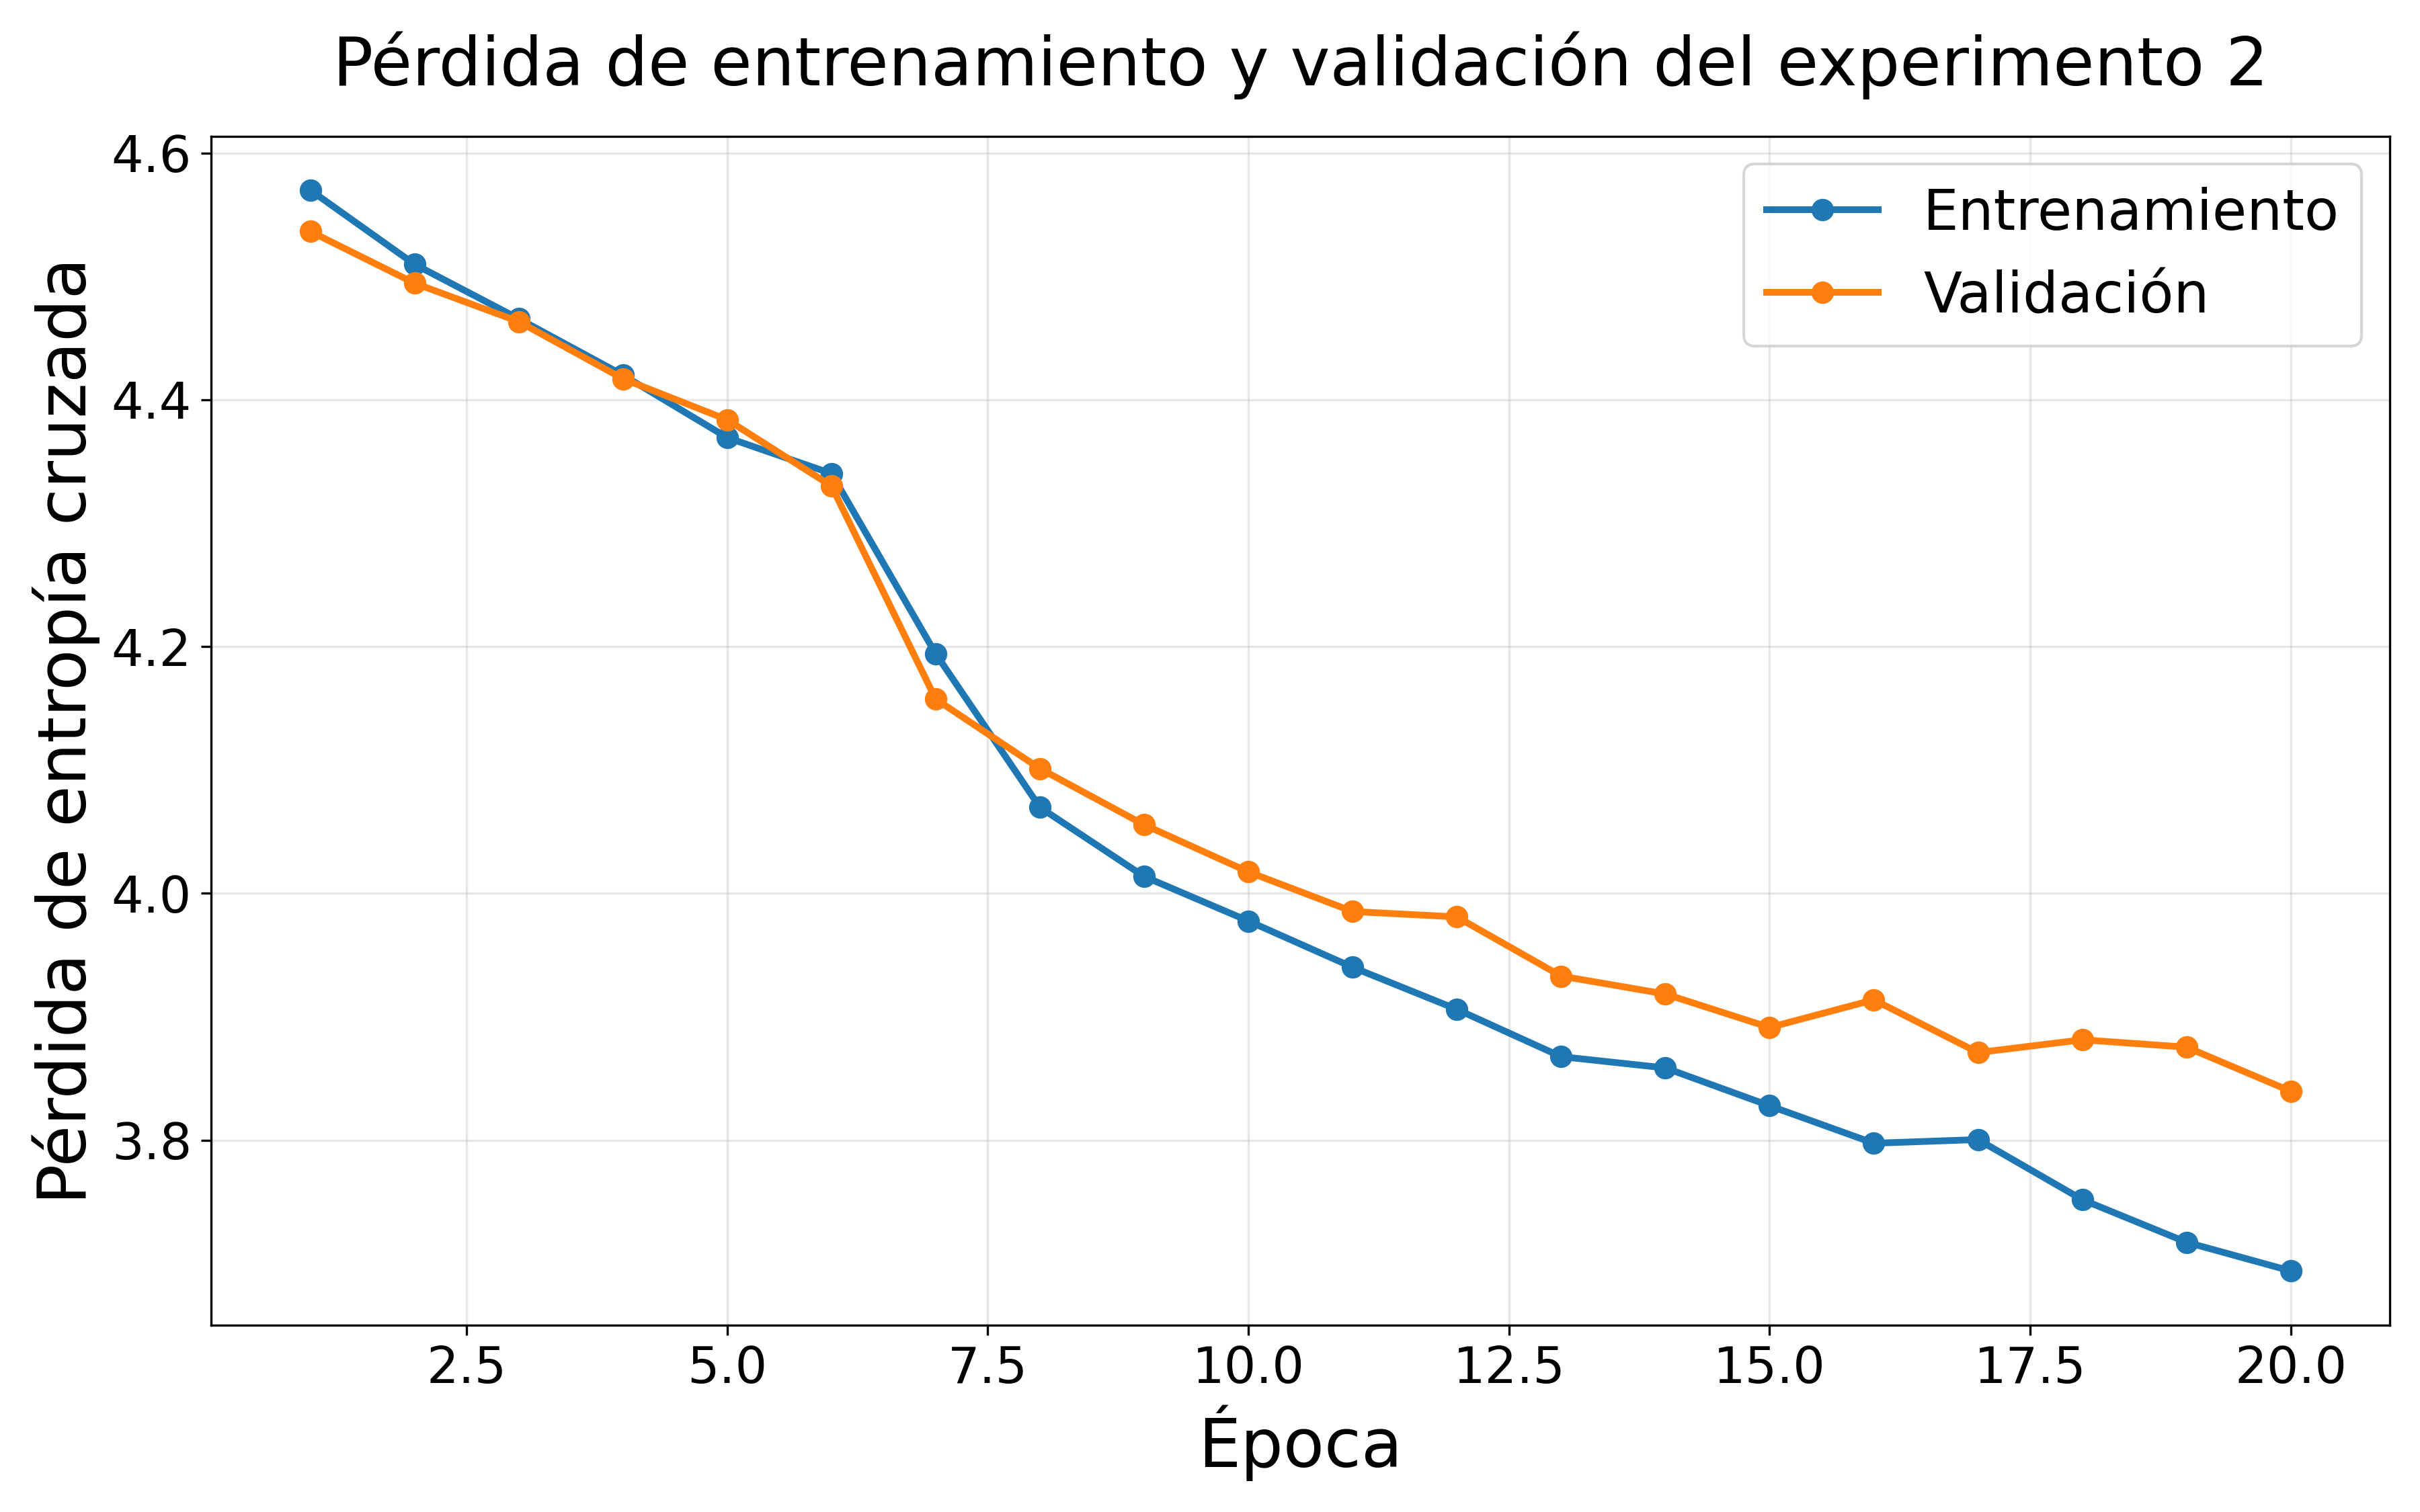
\includegraphics[width=0.55\linewidth]{figures/Experiments_logs/loss_curve_04-22.png}
    \caption{Primer experimento con la arquitectura híbrida. La pérdida ya no queda tan cerca del comportamiento aleatorio inicial.}
    \label{fig:loss_curve_04-22}
\end{figure}

\begin{table}[H]
\centering
\small
\begin{tabular}{lcccc}
\toprule
\textbf{Experimento} & \textbf{Mejor acc. eval} & \textbf{Época} & \textbf{Mejor eval loss} & \textbf{Eval loss final} \\
\midrule
\texttt{2} & 13,60\% & 47 & 3,5593 & 5,1254 \\
\bottomrule
\end{tabular}
\caption{Resumen del primer experimento relevante con \texttt{HybridCustomTTN}.}
\label{tab:hybridttn_inicial}
\end{table}

Este resultado confirmó la hipótesis 1, ya que el modelo dejó de tener un comportamiento prácticamente aleatorio. La precisión subió de 3,58\% a 13,60\%, y la mejor \textit{eval loss} bajó de 4,5153 a 3,5593. La mejora era clara, pero también apareció una señal nueva; al avanzar el entrenamiento, la pérdida de evaluación volvía a empeorar.

Para entender mejor esta tendencia se repitió el experimento durante más épocas:

\begin{figure}[H]
    \centering
    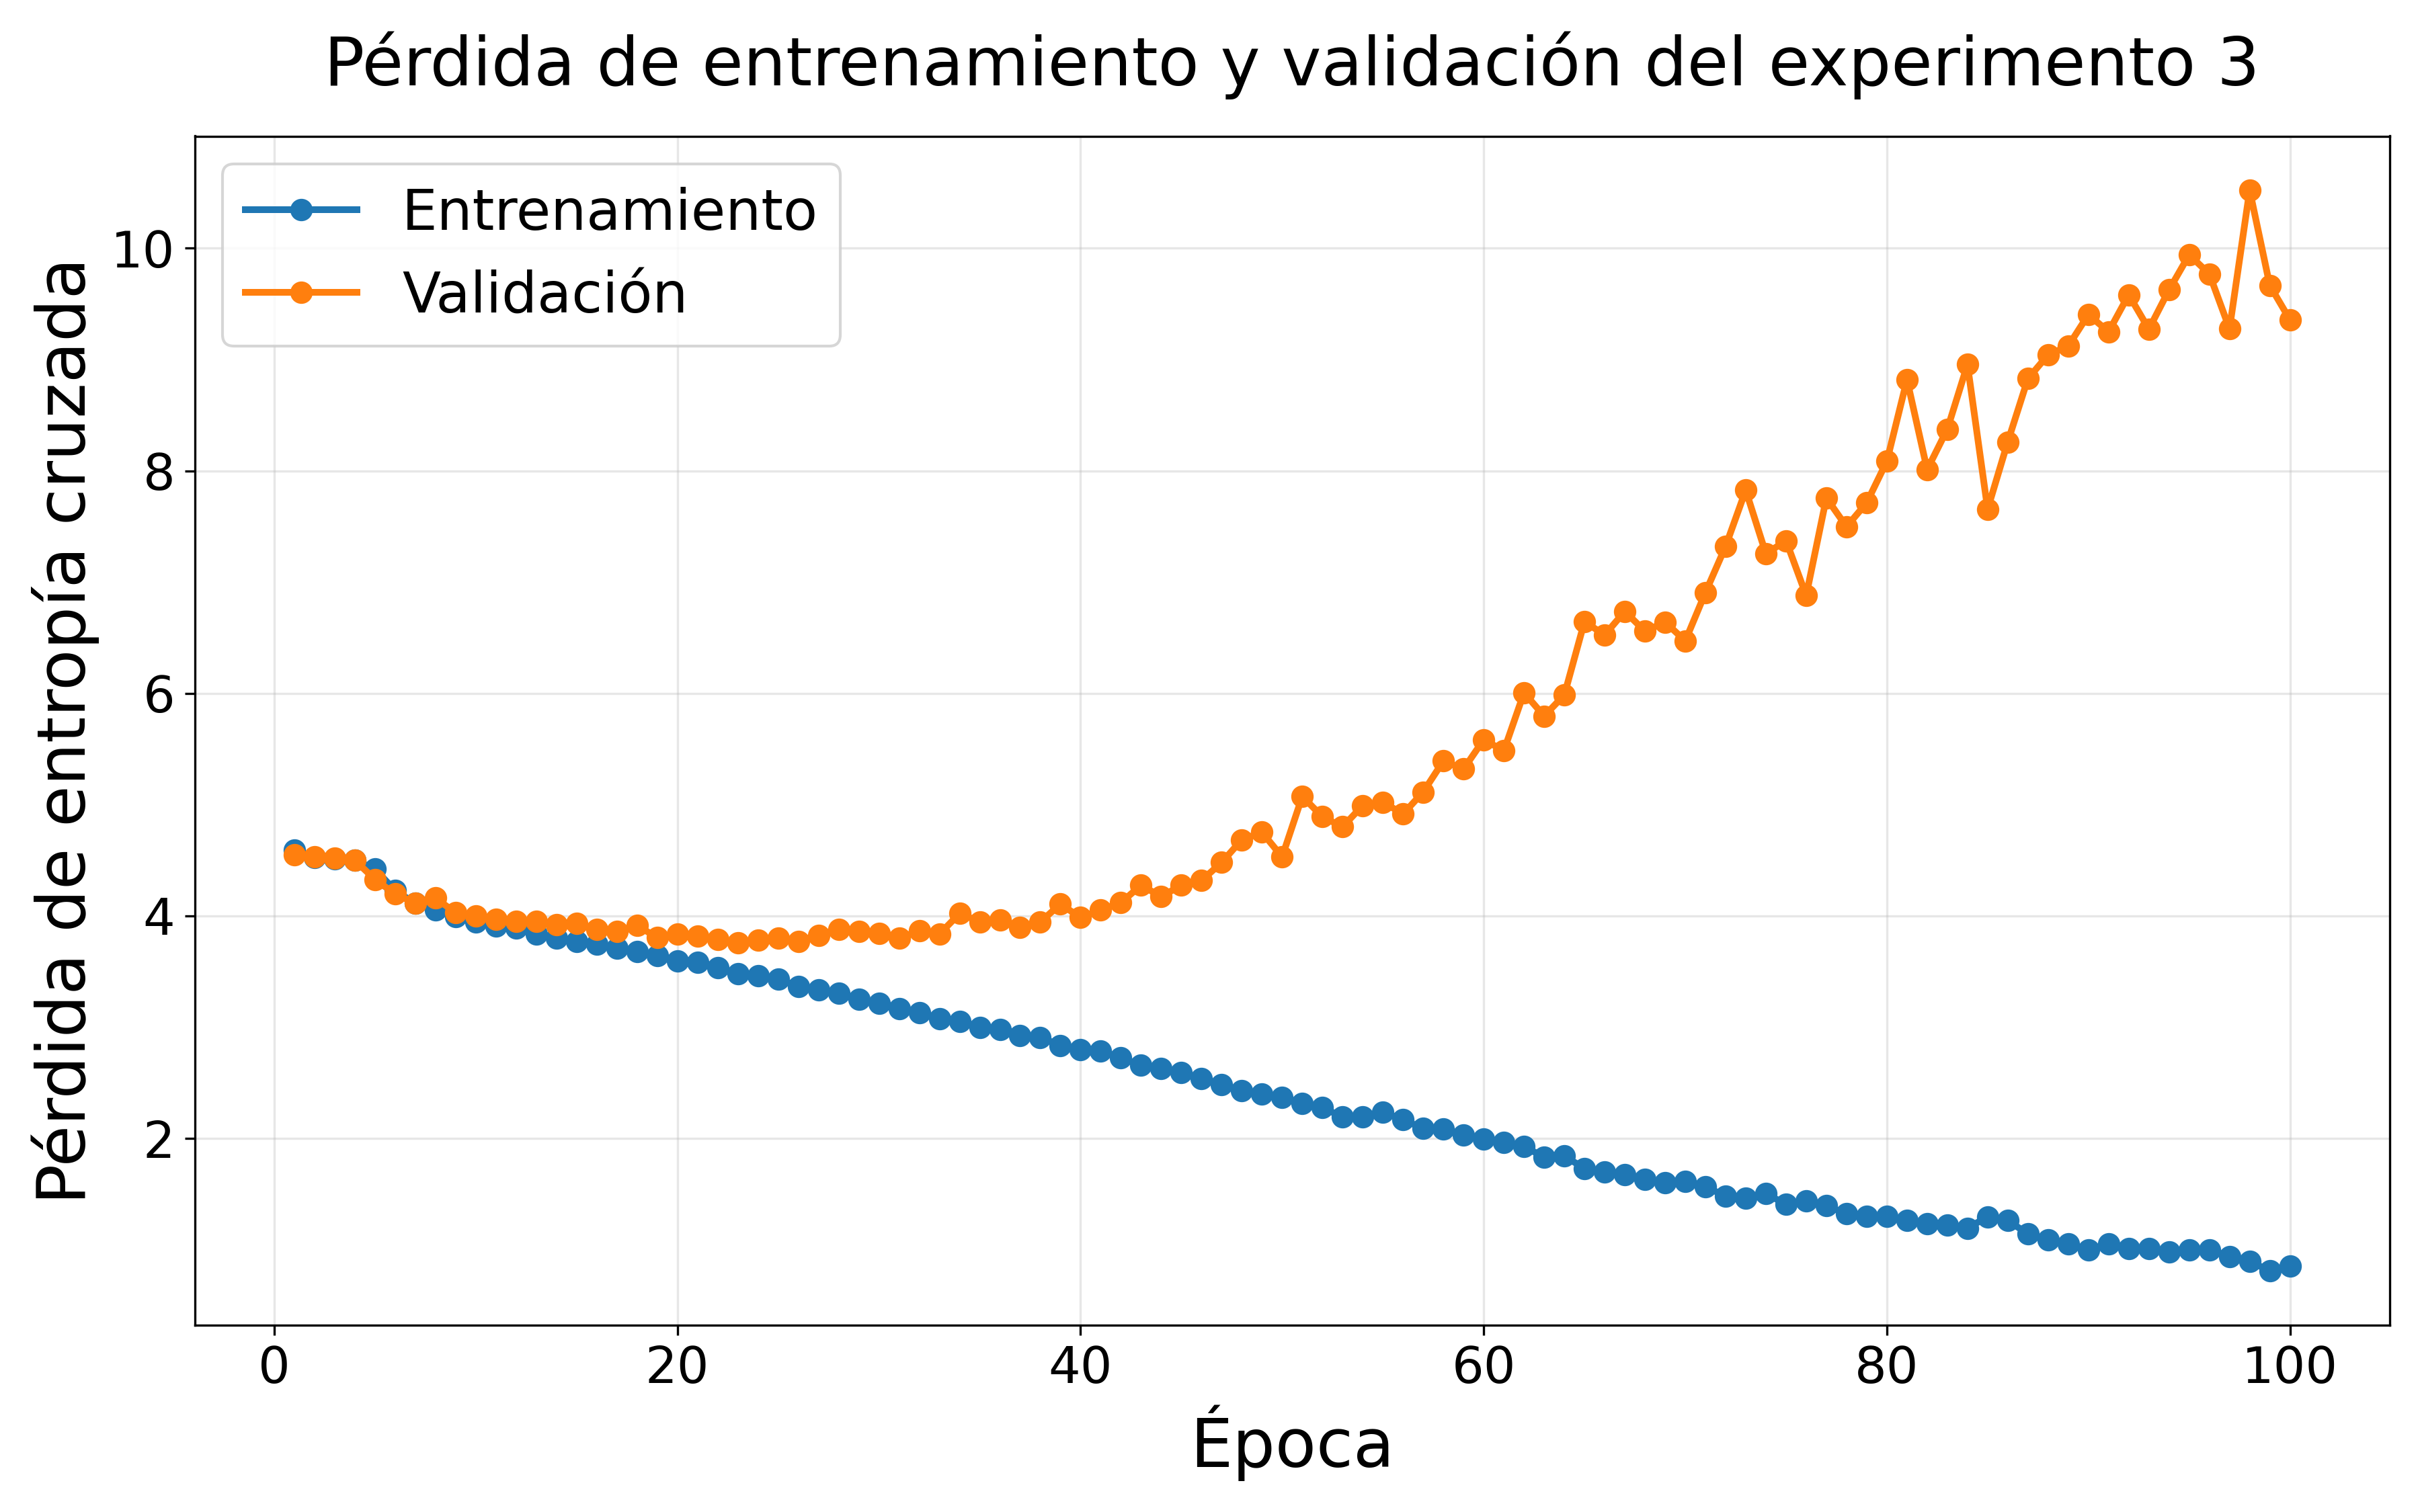
\includegraphics[width=0.55\linewidth]{figures/Experiments_logs/loss_curve_04-27.png}
    \caption{Experimento largo con \texttt{HybridCustomTTN} sobre Flowers102.}
    \label{fig:loss_curve_04-27}
\end{figure}

\begin{table}[H]
\centering
\small
\begin{tabular}{lccccc}
\toprule
\textbf{Experimento} & \textbf{Acc. eval} & \textbf{Época} & \textbf{Train loss} & \textbf{Eval loss} & \textbf{Acc. final} \\
\midrule
\texttt{3} & 12,46\% & 54 & 1,3295 & 8,2368 & 8,55\% \\
\bottomrule
\end{tabular}
\caption{Resumen del experimento largo con \texttt{HybridCustomTTN}.}
\label{tab:hybridttn_largo}
\end{table}

Aquí ya se ve mucho mejor el problema. La \textit{train loss} baja de forma sostenida hasta 1,3295, así que el modelo sí aprende el conjunto de entrenamiento. Sin embargo, la \textit{eval loss} sube hasta 8,2368 y la precisión final cae al 8,55\%. Esto es una señal clara de \textit{overfitting}, el modelo se adapta al entrenamiento, pero no generaliza bien a imágenes nuevas.

\subsection{Hipótesis 2}

La segunda hipótesis fue que el modelo estaba perdiendo demasiada información espacial de la imagen. Hasta ese momento se usaba \texttt{PatchEmbedding}. Para imágenes de $224\times224$ y \texttt{patch\_size=16}, la imagen se divide en una rejilla de $14\times14$, es decir, 196 posiciones. Cada \textit{patch} se proyecta a una dimensión \texttt{local\_dim} y se entrega a la TTN:

\begin{center}
\texttt{[B, 3, 224, 224] -> [B, 196, local\_dim]}.
\end{center}

El problema es que, en las primeras pruebas, \texttt{local\_dim} era muy pequeña. Se estaba comprimiendo cada \textit{patch} de la imagen a muy pocos números antes de que el modelo pudiera procesar bien la localidad espacial. El zigzag ayudaba a ordenar la secuencia, pero no recuperaba la estructura 2D original. Por eso el siguiente cambio fue introducir un \textit{embedding} que procesara la imagen como mapa bidimensional antes de aplanarla.

\section{Cambio del embedding a AIM}

El cambio a \texttt{AIMPatchEmbedding} nace de la hipótesis 2. El objetivo era conservar más información espacial antes de entregar la imagen a la TTN. Para ello se incorporó un \textit{front-end} inspirado en los bloques AIM de \textit{Deep Tree Tensor Networks for Image Recognition} \citebox{nie2025deeptreetensornetworks}.

\begin{center}
\texttt{imagen -> stem CNN -> AIM2D -> Conv2d 1x1 -> flatten + zigzag -> HybridCustomTTN}
\end{center}

El bloque AIM2D combina dos ramas lineales mediante producto elemento a elemento. Si ambas ramas son lineales en la entrada, su producto introduce interacciones bilineales. Esta idea encaja muy bien con las redes tensoriales, porque introduce interacciones multiplicativas estructuradas antes de pasar a la TTN.

En términos de dimensiones, con imágenes de $224\times224$ y \texttt{patch\_size=16}, el front-end reduce la imagen a una rejilla $14\times14$. Después, una convolución $1\times1$ proyecta los canales a \texttt{local\_dim}, y finalmente la rejilla se aplana:

\begin{center}
\texttt{[B, 3, 224, 224] -> [B, local\_dim, 14, 14] -> [B, 196, local\_dim]}.
\end{center}

El primer experimento con AIM durante 50 épocas fue:

\begin{figure}[H]
    \centering
    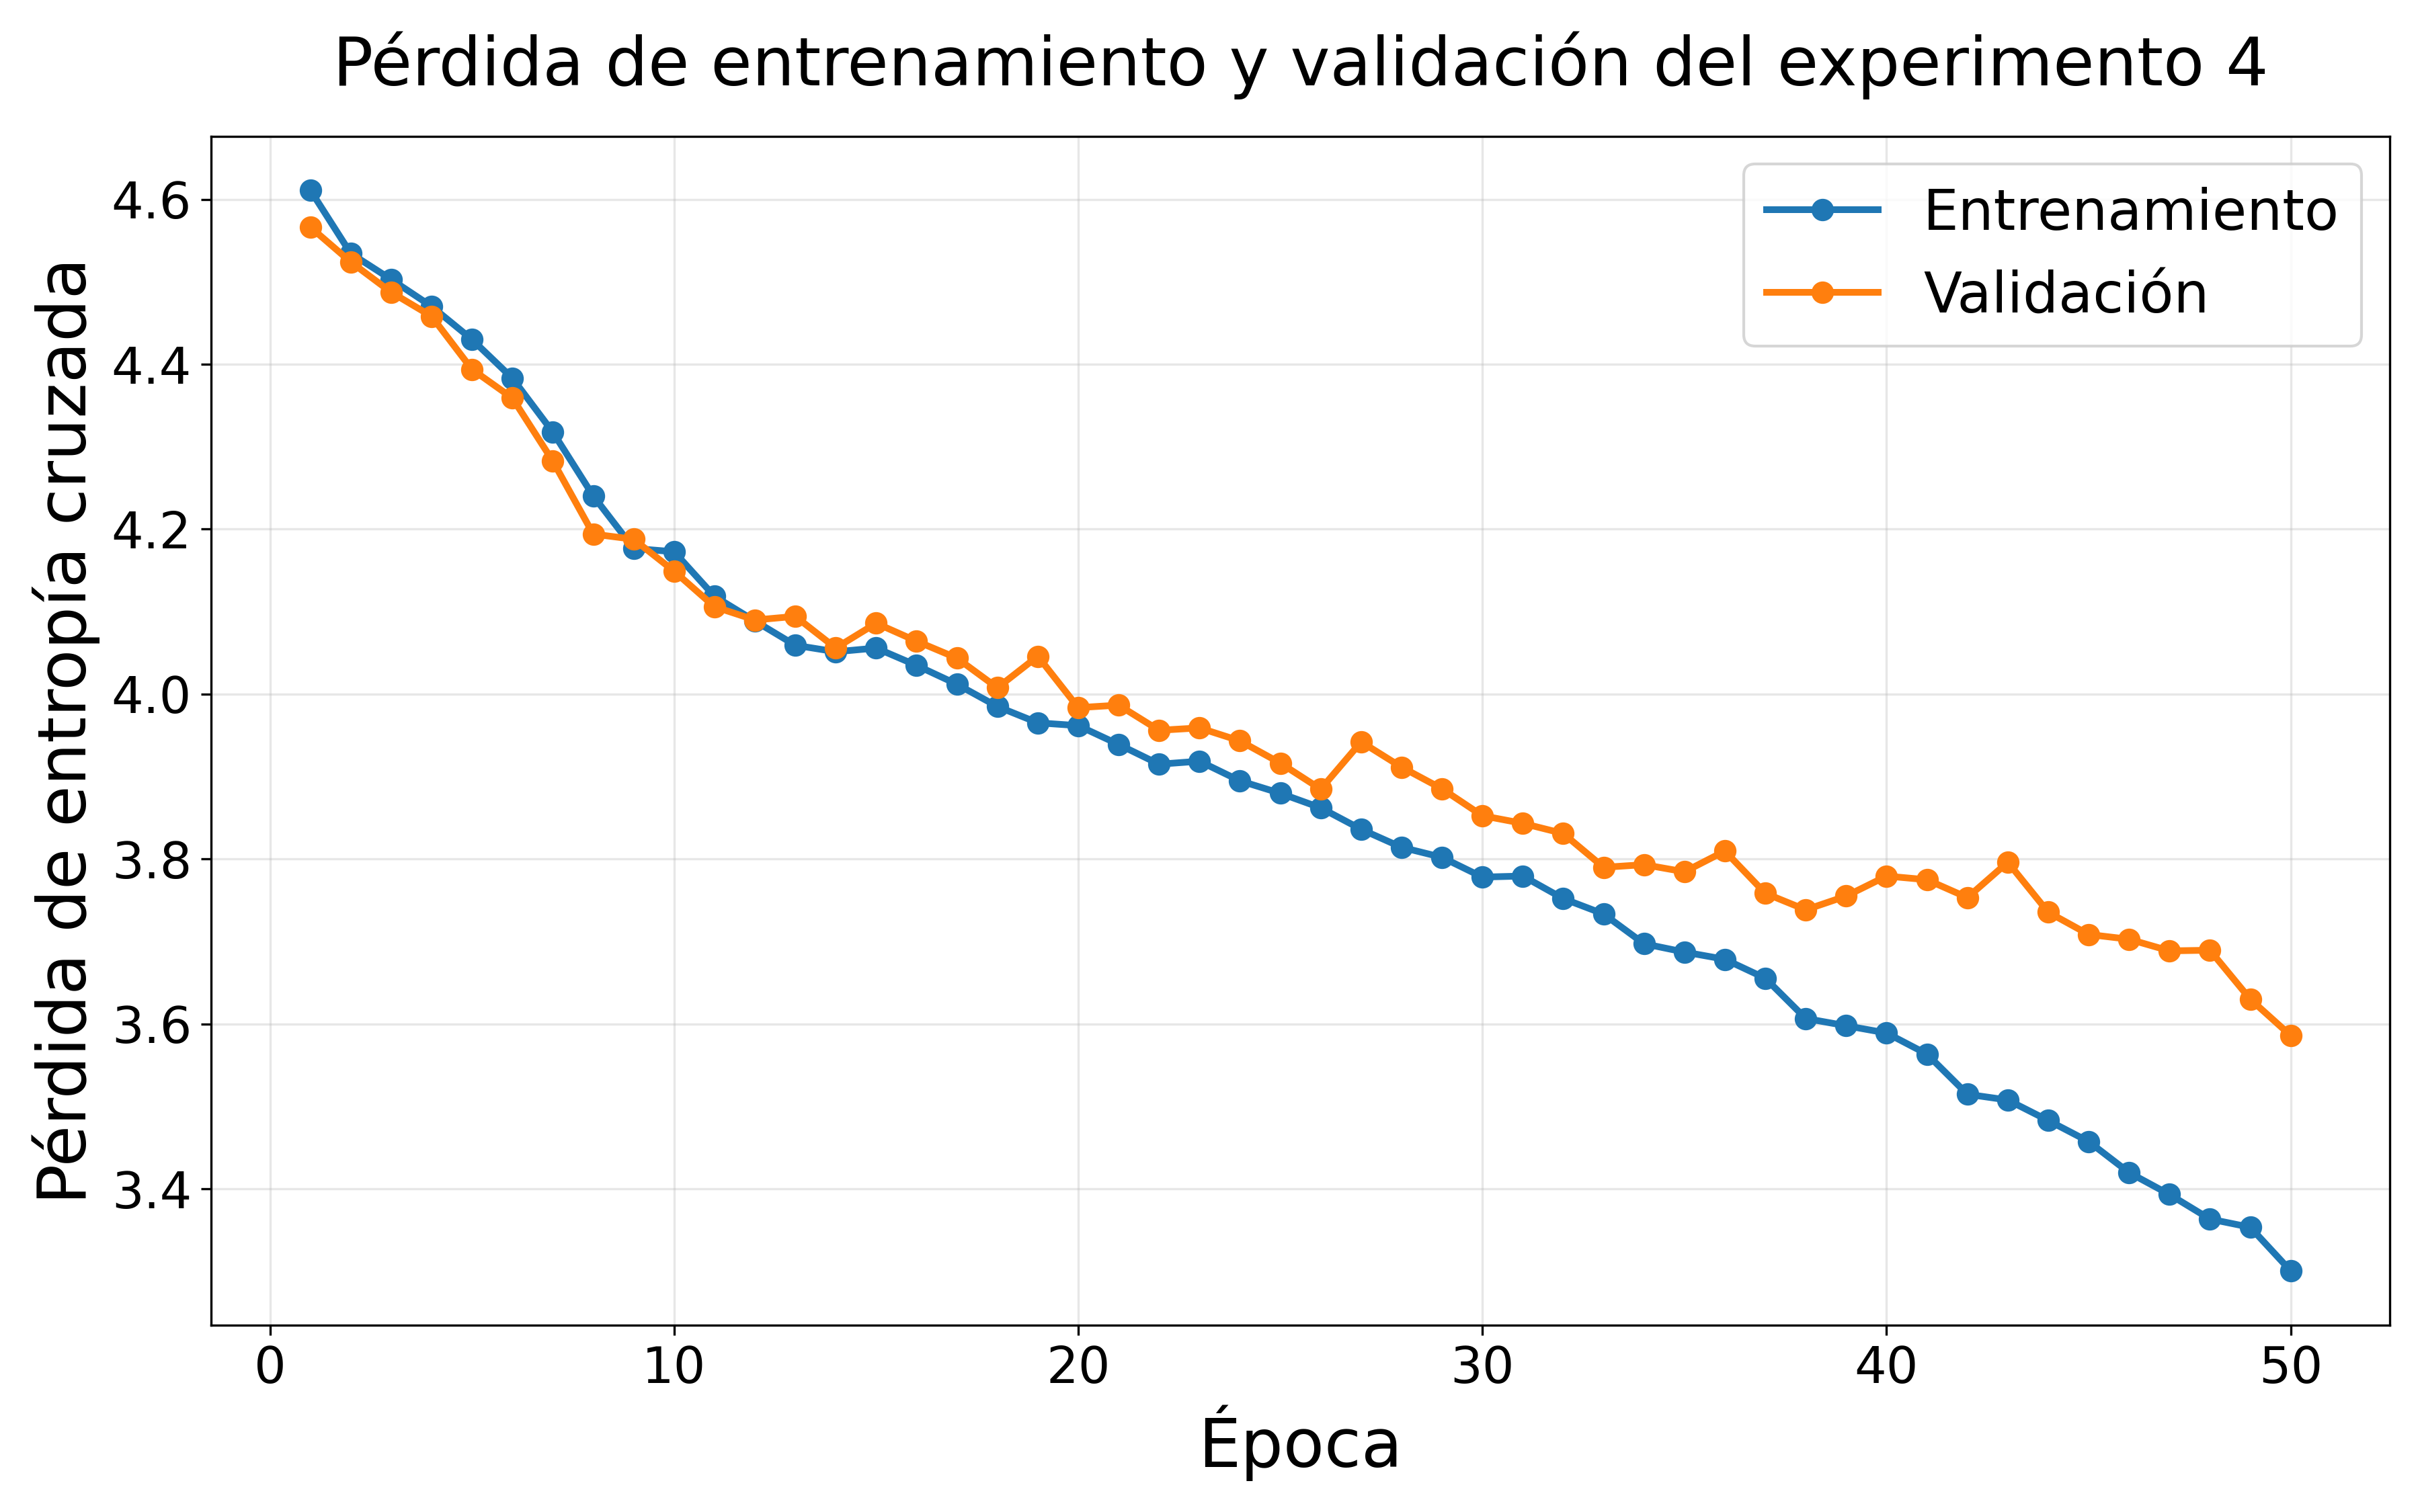
\includegraphics[width=0.55\linewidth]{figures/Experiments_logs/loss_curve_04-28-50.png}
    \caption{Experimento con \texttt{AIMPatchEmbedding} durante 50 épocas.}
    \label{fig:loss_curve_04-28-50}
\end{figure}

\begin{table}[H]
\centering
\small
\begin{tabular}{lcccc}
\toprule
\textbf{Experimento} & \textbf{Épocas} & \textbf{Mejor acc. eval} & \textbf{Mejor eval loss} & \textbf{Acc. final} \\
\midrule
\texttt{4} & 50 & 14,01\% & 3,5859 & 14,01\% \\
\bottomrule
\end{tabular}
\caption{Primer resultado con \texttt{AIMPatchEmbedding}.}
\label{tab:aim_50}
\end{table}

El resultado fue positivo porque la pérdida seguía bajando y no se observaba una separación tan violenta entre entrenamiento y evaluación. Para compararlo mejor con los experimentos anteriores, se repitió con 100 épocas:

\begin{figure}[H]
    \centering
    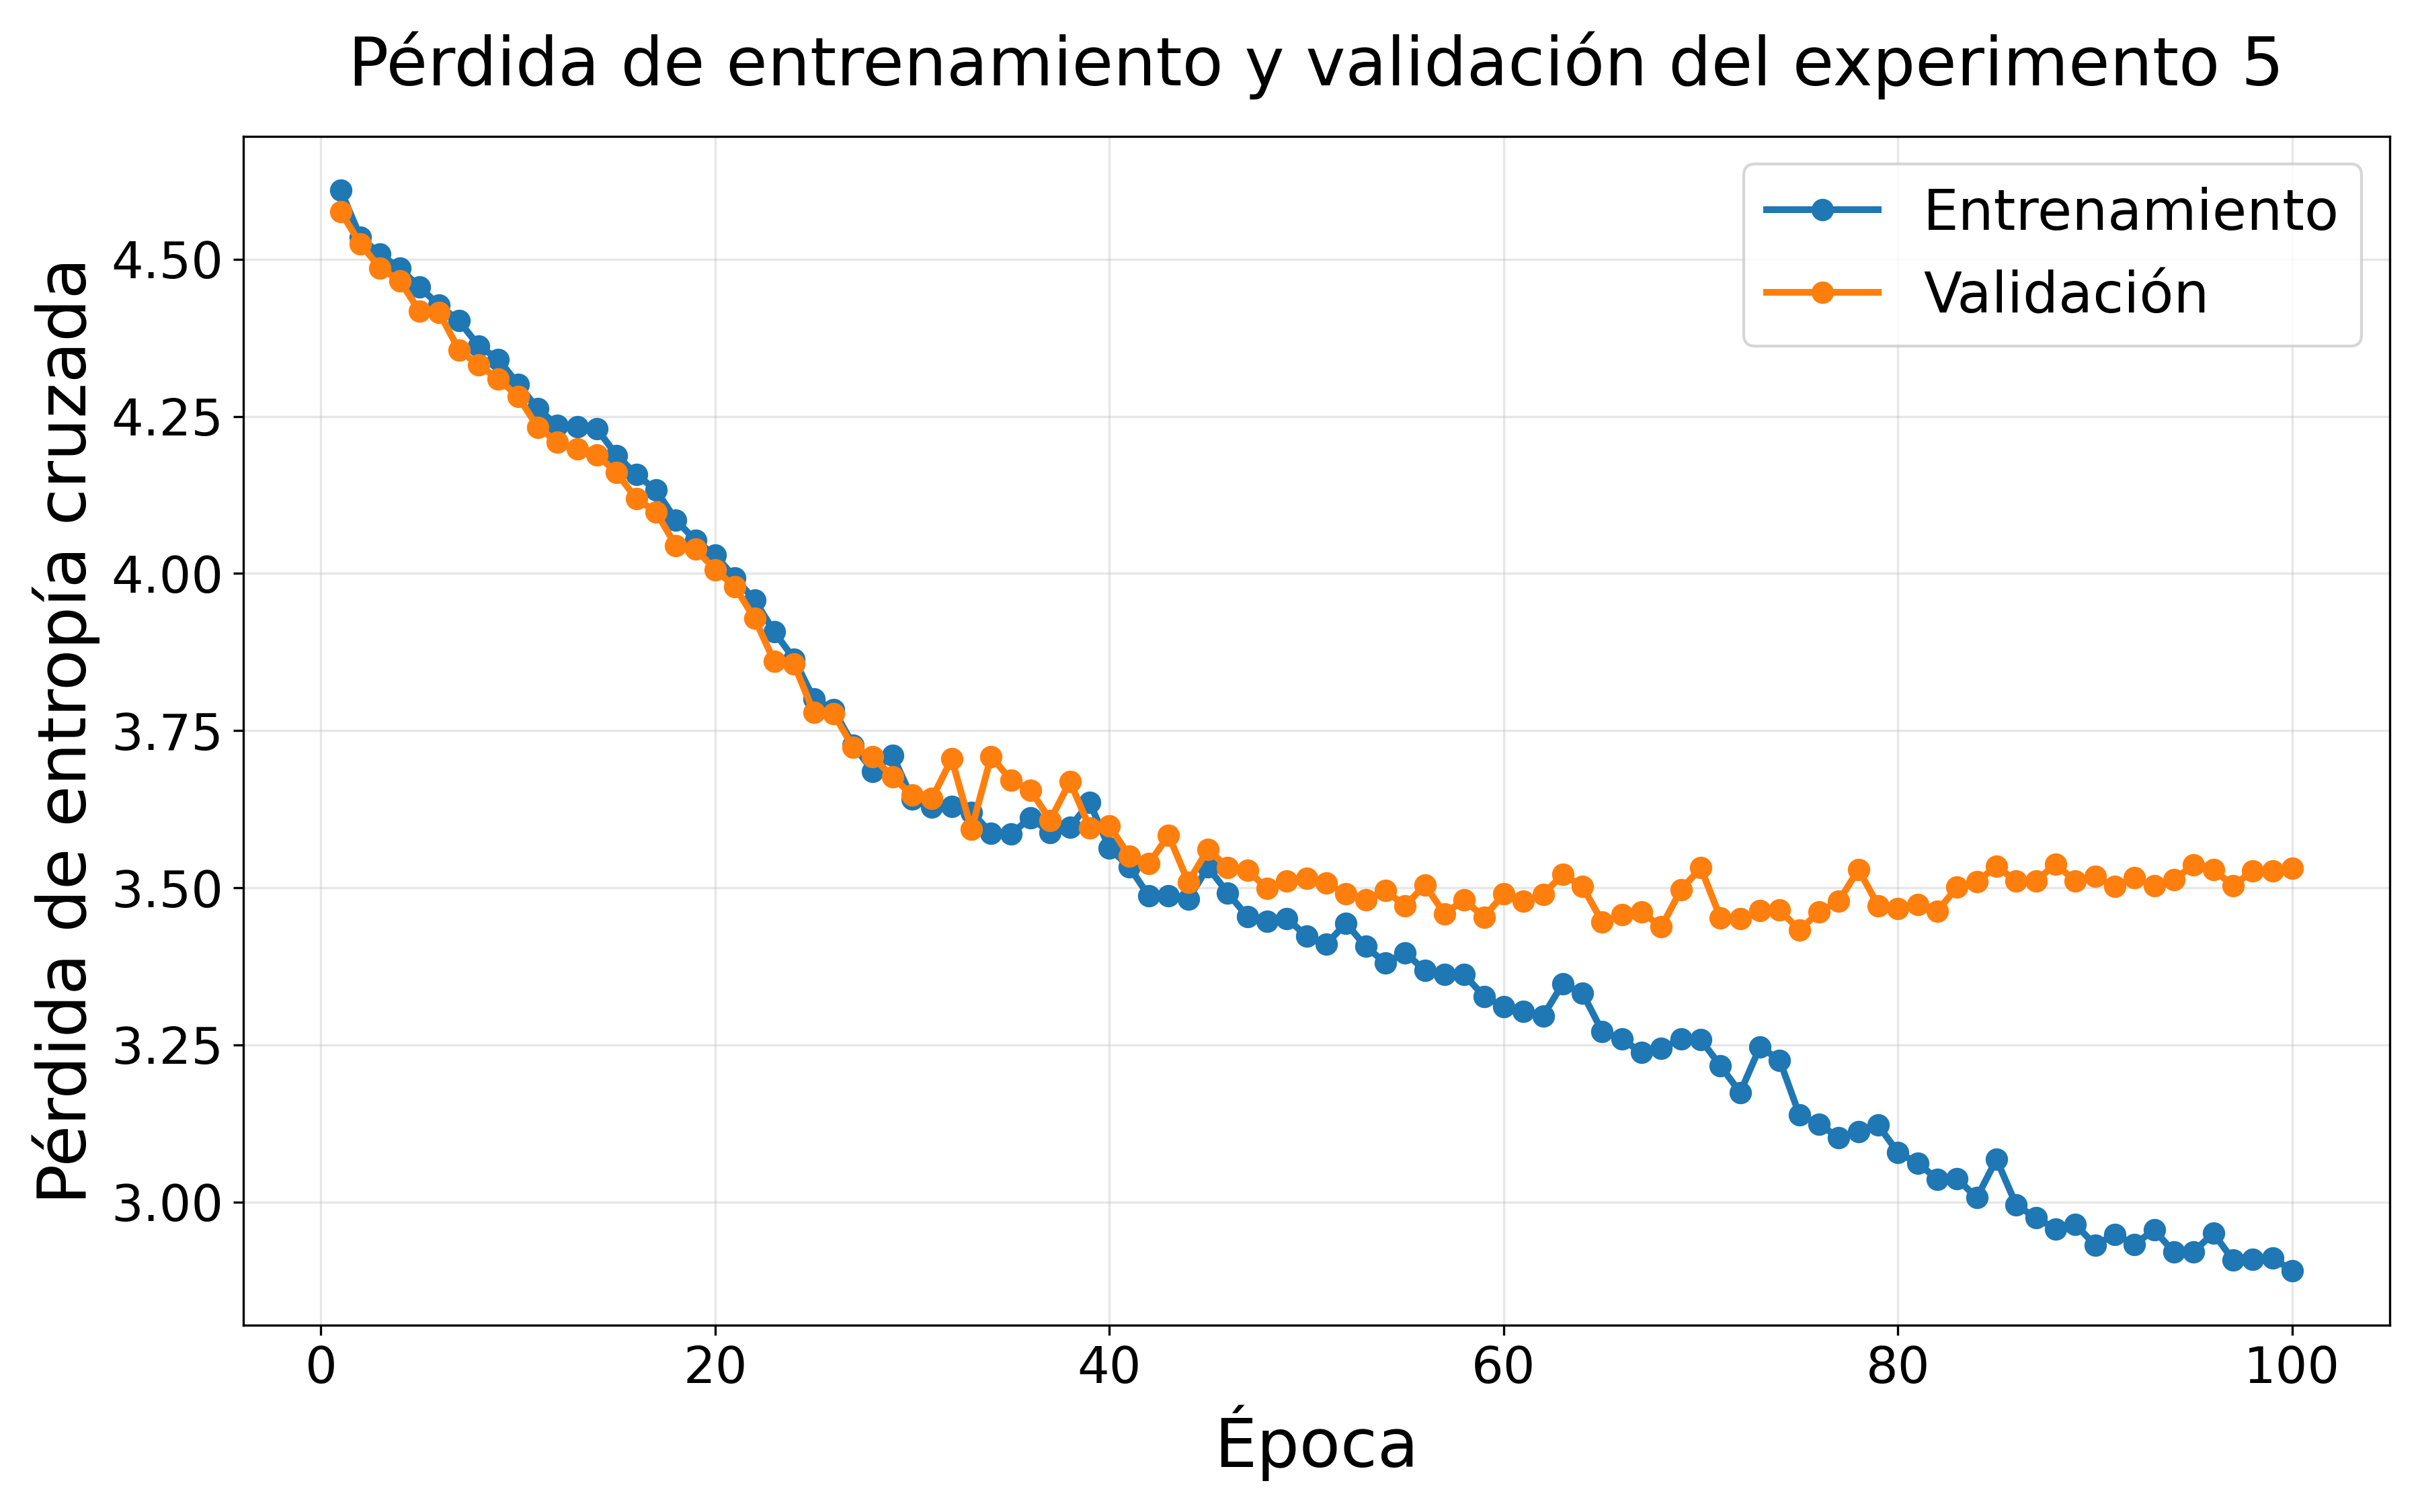
\includegraphics[width=0.55\linewidth]{figures/Experiments_logs/loss_curve_04-28-100.png}
    \caption{Experimento con \texttt{AIMPatchEmbedding} durante 100 épocas.}
    \label{fig:loss_curve_04-28-100}
\end{figure}

\begin{table}[H]
\centering
\small
\begin{tabular}{lcccc}
\toprule
\textbf{Experimento} & \textbf{Épocas} & \textbf{Mejor acc. eval} & \textbf{Mejor eval loss} & \textbf{Eval loss final} \\
\midrule
\texttt{5} & 100 & 15,88\% & 3,4330 & 3,5312 \\
\bottomrule
\end{tabular}
\caption{Resultado con AIM durante 100 épocas.}
\label{tab:aim_100}
\end{table}

Comparado con \figref{fig:loss_curve_04-27}, el \textit{overfitting} ya no era tan agresivo. Antes la \textit{eval loss} acababa en 8,2368, mientras que con AIM se mantuvo alrededor de 3,5312. La precisión seguía siendo baja, pero el comportamiento del entrenamiento era más sano. Esto indicaba que AIM no era una solución mágica, pero sí estaba atacando el problema correcto.

El siguiente paso fue aplicar \textit{data augmentation}. Esta técnica consiste en generar variaciones de las imágenes durante el entrenamiento, por ejemplo con cambios de recorte, color, orientación o borrado parcial. La idea es que el modelo no memorice una única versión de cada imagen, sino que aprenda rasgos más generales.

\begin{figure}[H]
    \centering

    \begin{subfigure}{0.45\textwidth}
        \centering
        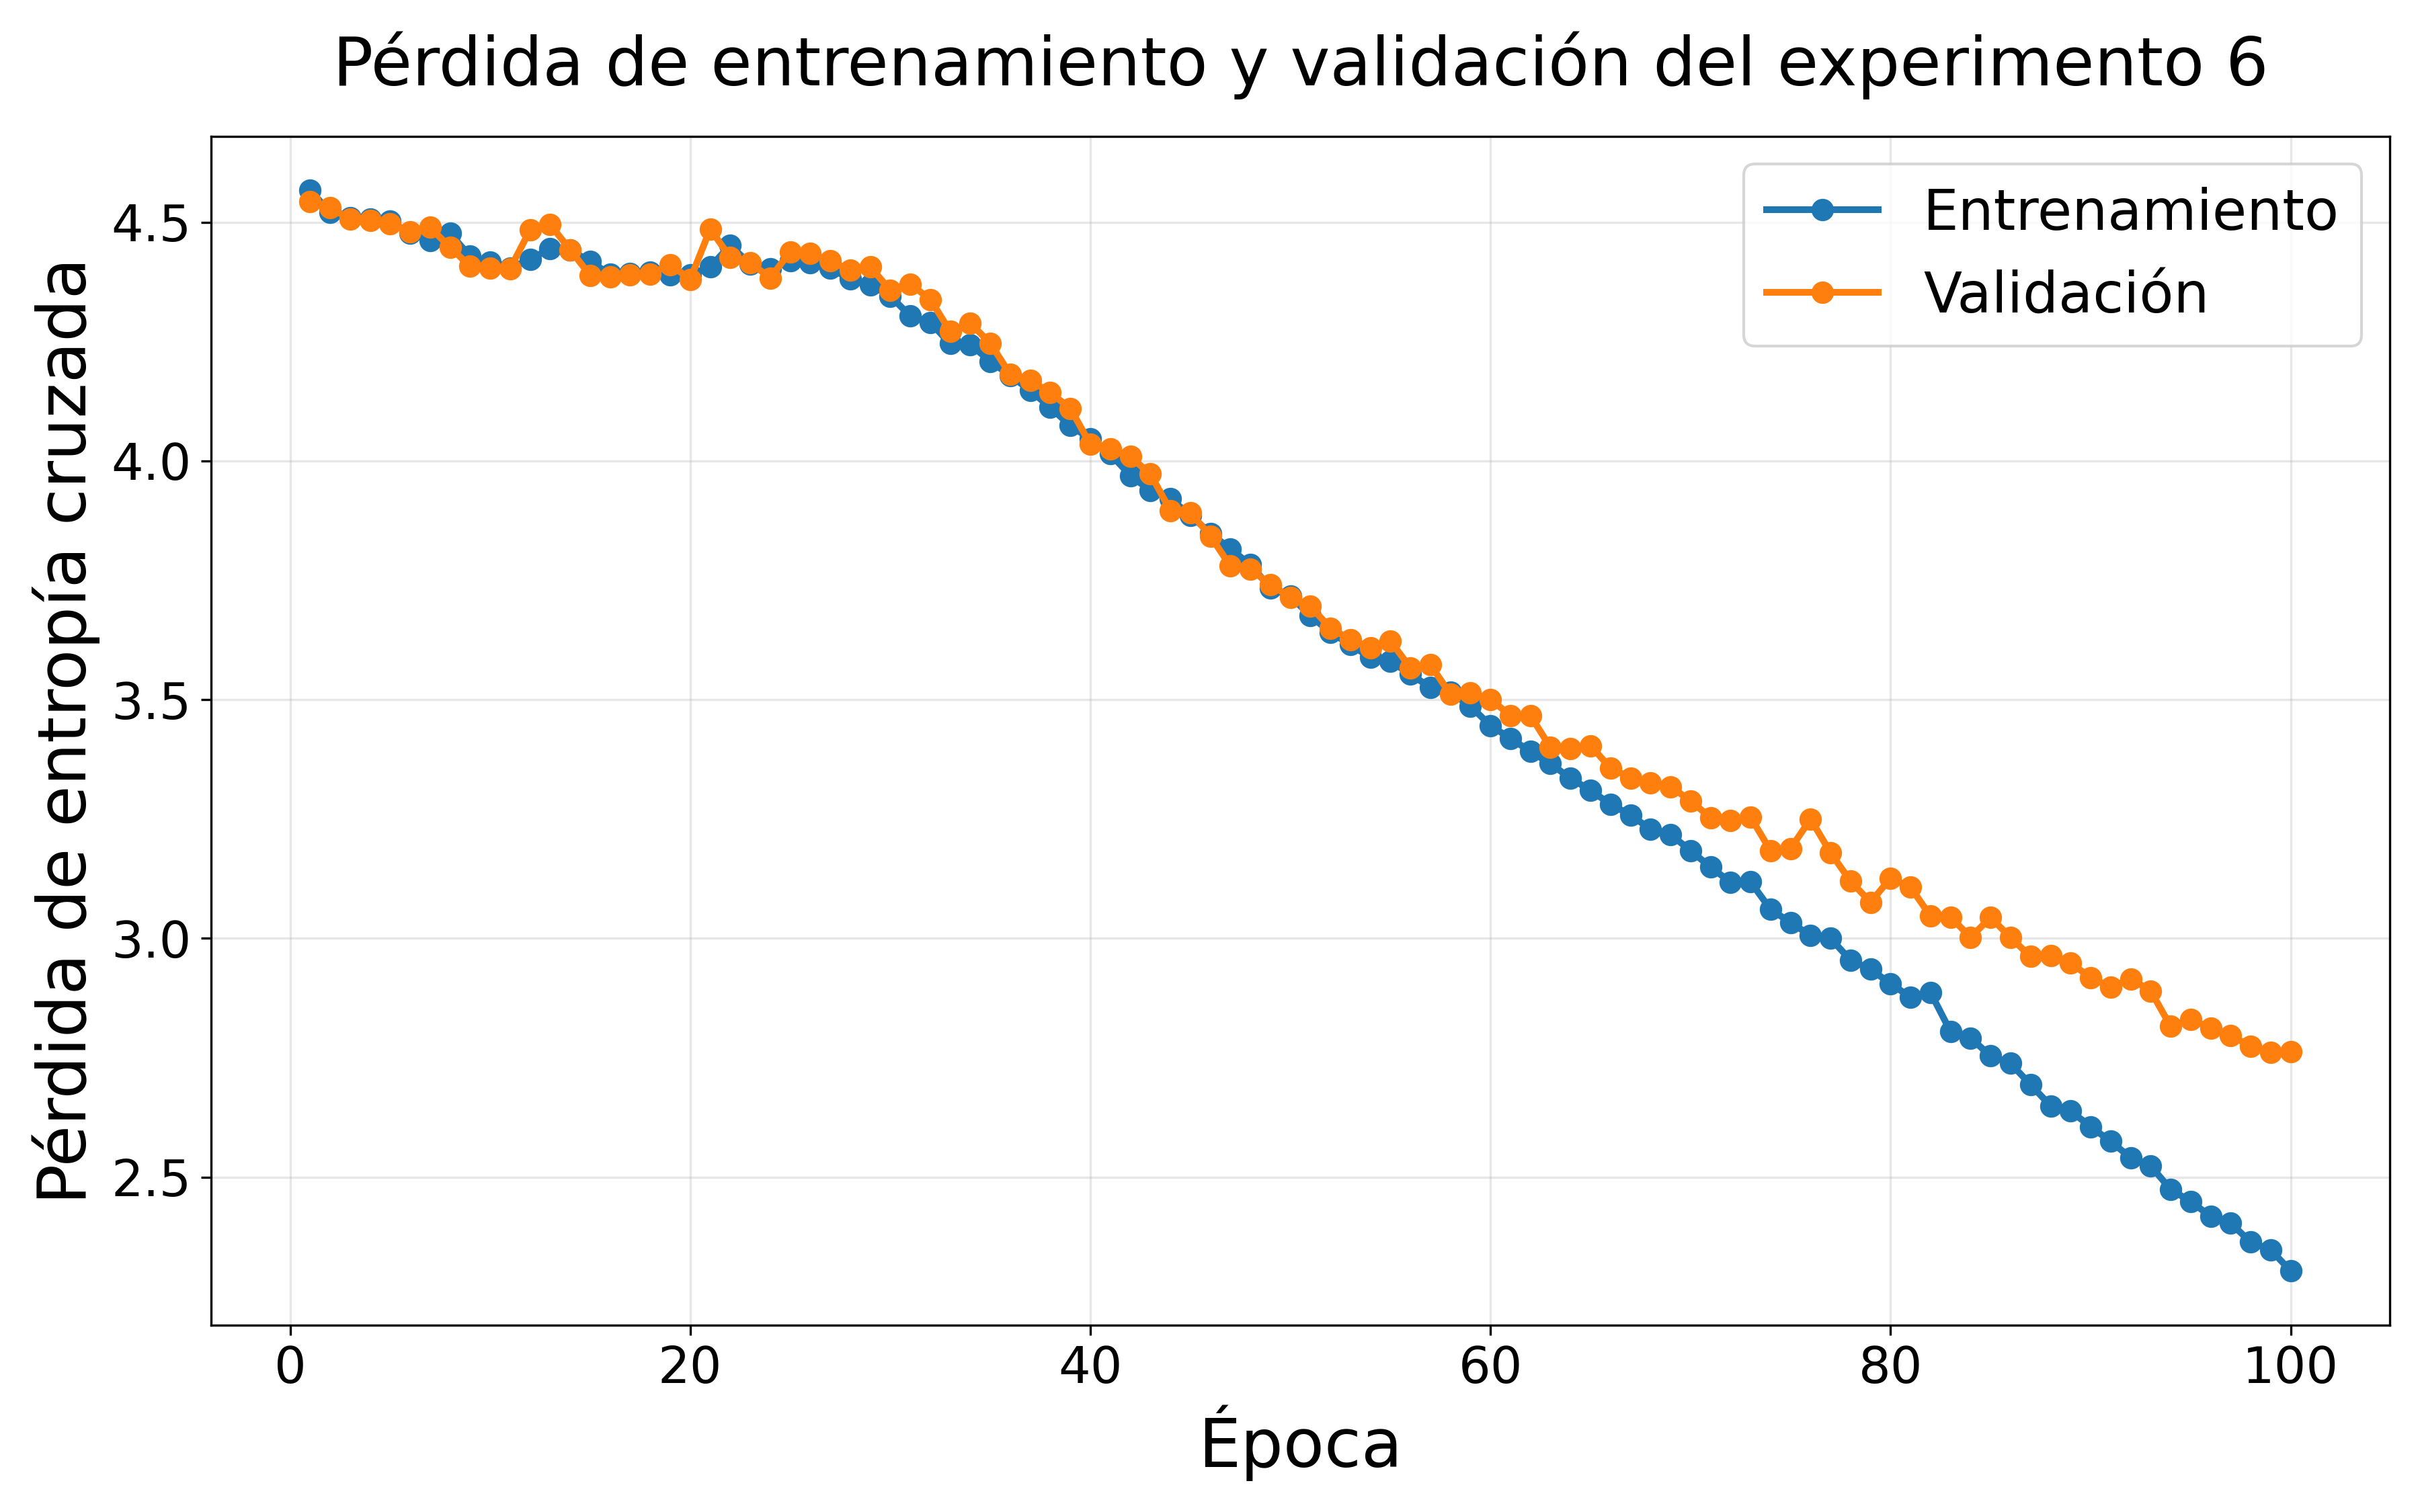
\includegraphics[width=\textwidth]{figures/Experiments_logs/loss_curve_04-30-0011.png}
        \caption{}
        \label{fig:loss_curve_04-30-0011}
    \end{subfigure}
    \hfill
    \begin{subfigure}{0.45\textwidth}
        \centering
        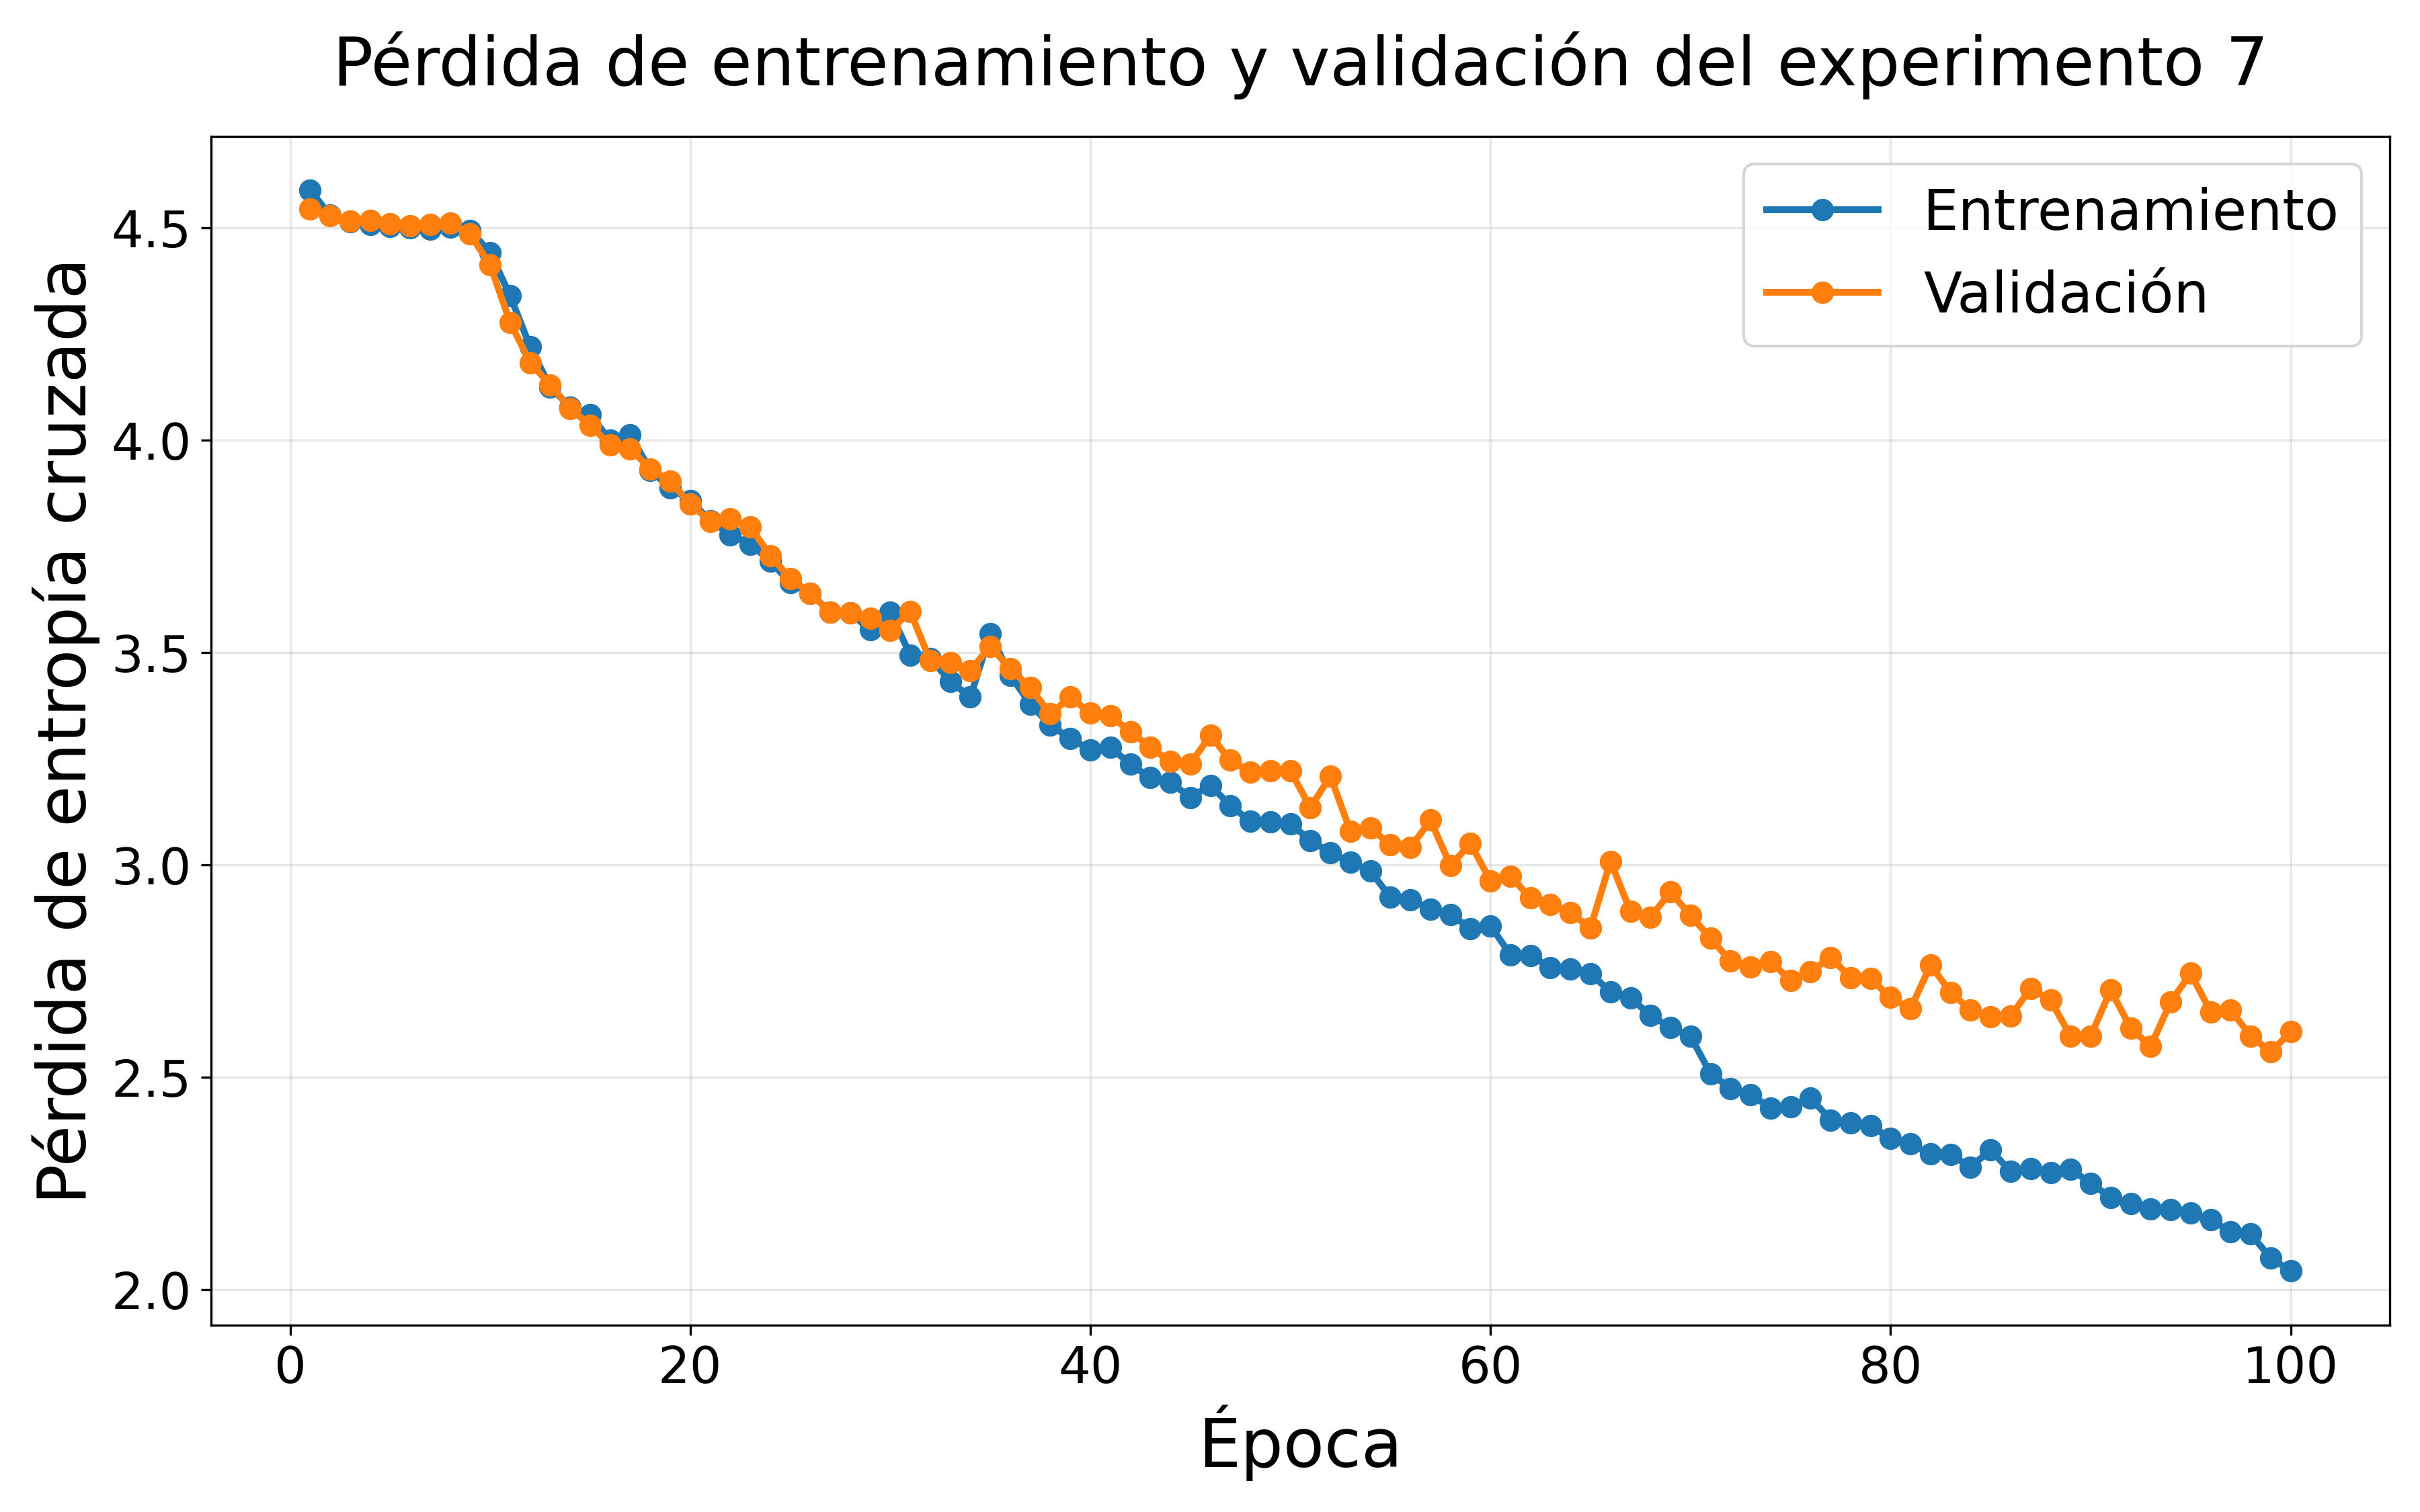
\includegraphics[width=\textwidth]{figures/Experiments_logs/loss_curve_04-30-0021.png}
        \caption{}
        \label{fig:loss_curve_04-30-0021}
    \end{subfigure}

    \caption{Experimentos en Flowers102 con AIM y \textit{data augmentation}.}
    \label{fig:loss_curve_04-30-0011-0021}
\end{figure}

\begin{table}[H]
\centering
\small
\begin{tabular}{lcccc}
\toprule
\textbf{Experimento} & \textbf{Mejor acc. eval} & \textbf{Top-5 eval} & \textbf{Mejor eval loss} & \textbf{Acc. final} \\
\midrule
\texttt{6} & 30,13\% & 61,40\% & 2,7612 & 29,97\% \\
\texttt{7} & 33,96\% & 66,04\% & 2,5600 & 33,96\% \\
\bottomrule
\end{tabular}
\caption{Mejores resultados sobre Flowers102 después de añadir AIM y \textit{data augmentation}.}
\label{tab:flowers_aim_aug}
\end{table}

Aquí el cambio ya fue bastante más claro. La precisión subió hasta 33,96\% y el top-5 alcanzó 66,04\%. Aun así, la matriz de confusión mostraba que el modelo seguía confundiendo muchas clases.

\begin{figure}[H]
    \centering

    \begin{subfigure}{0.45\textwidth}
        \centering
        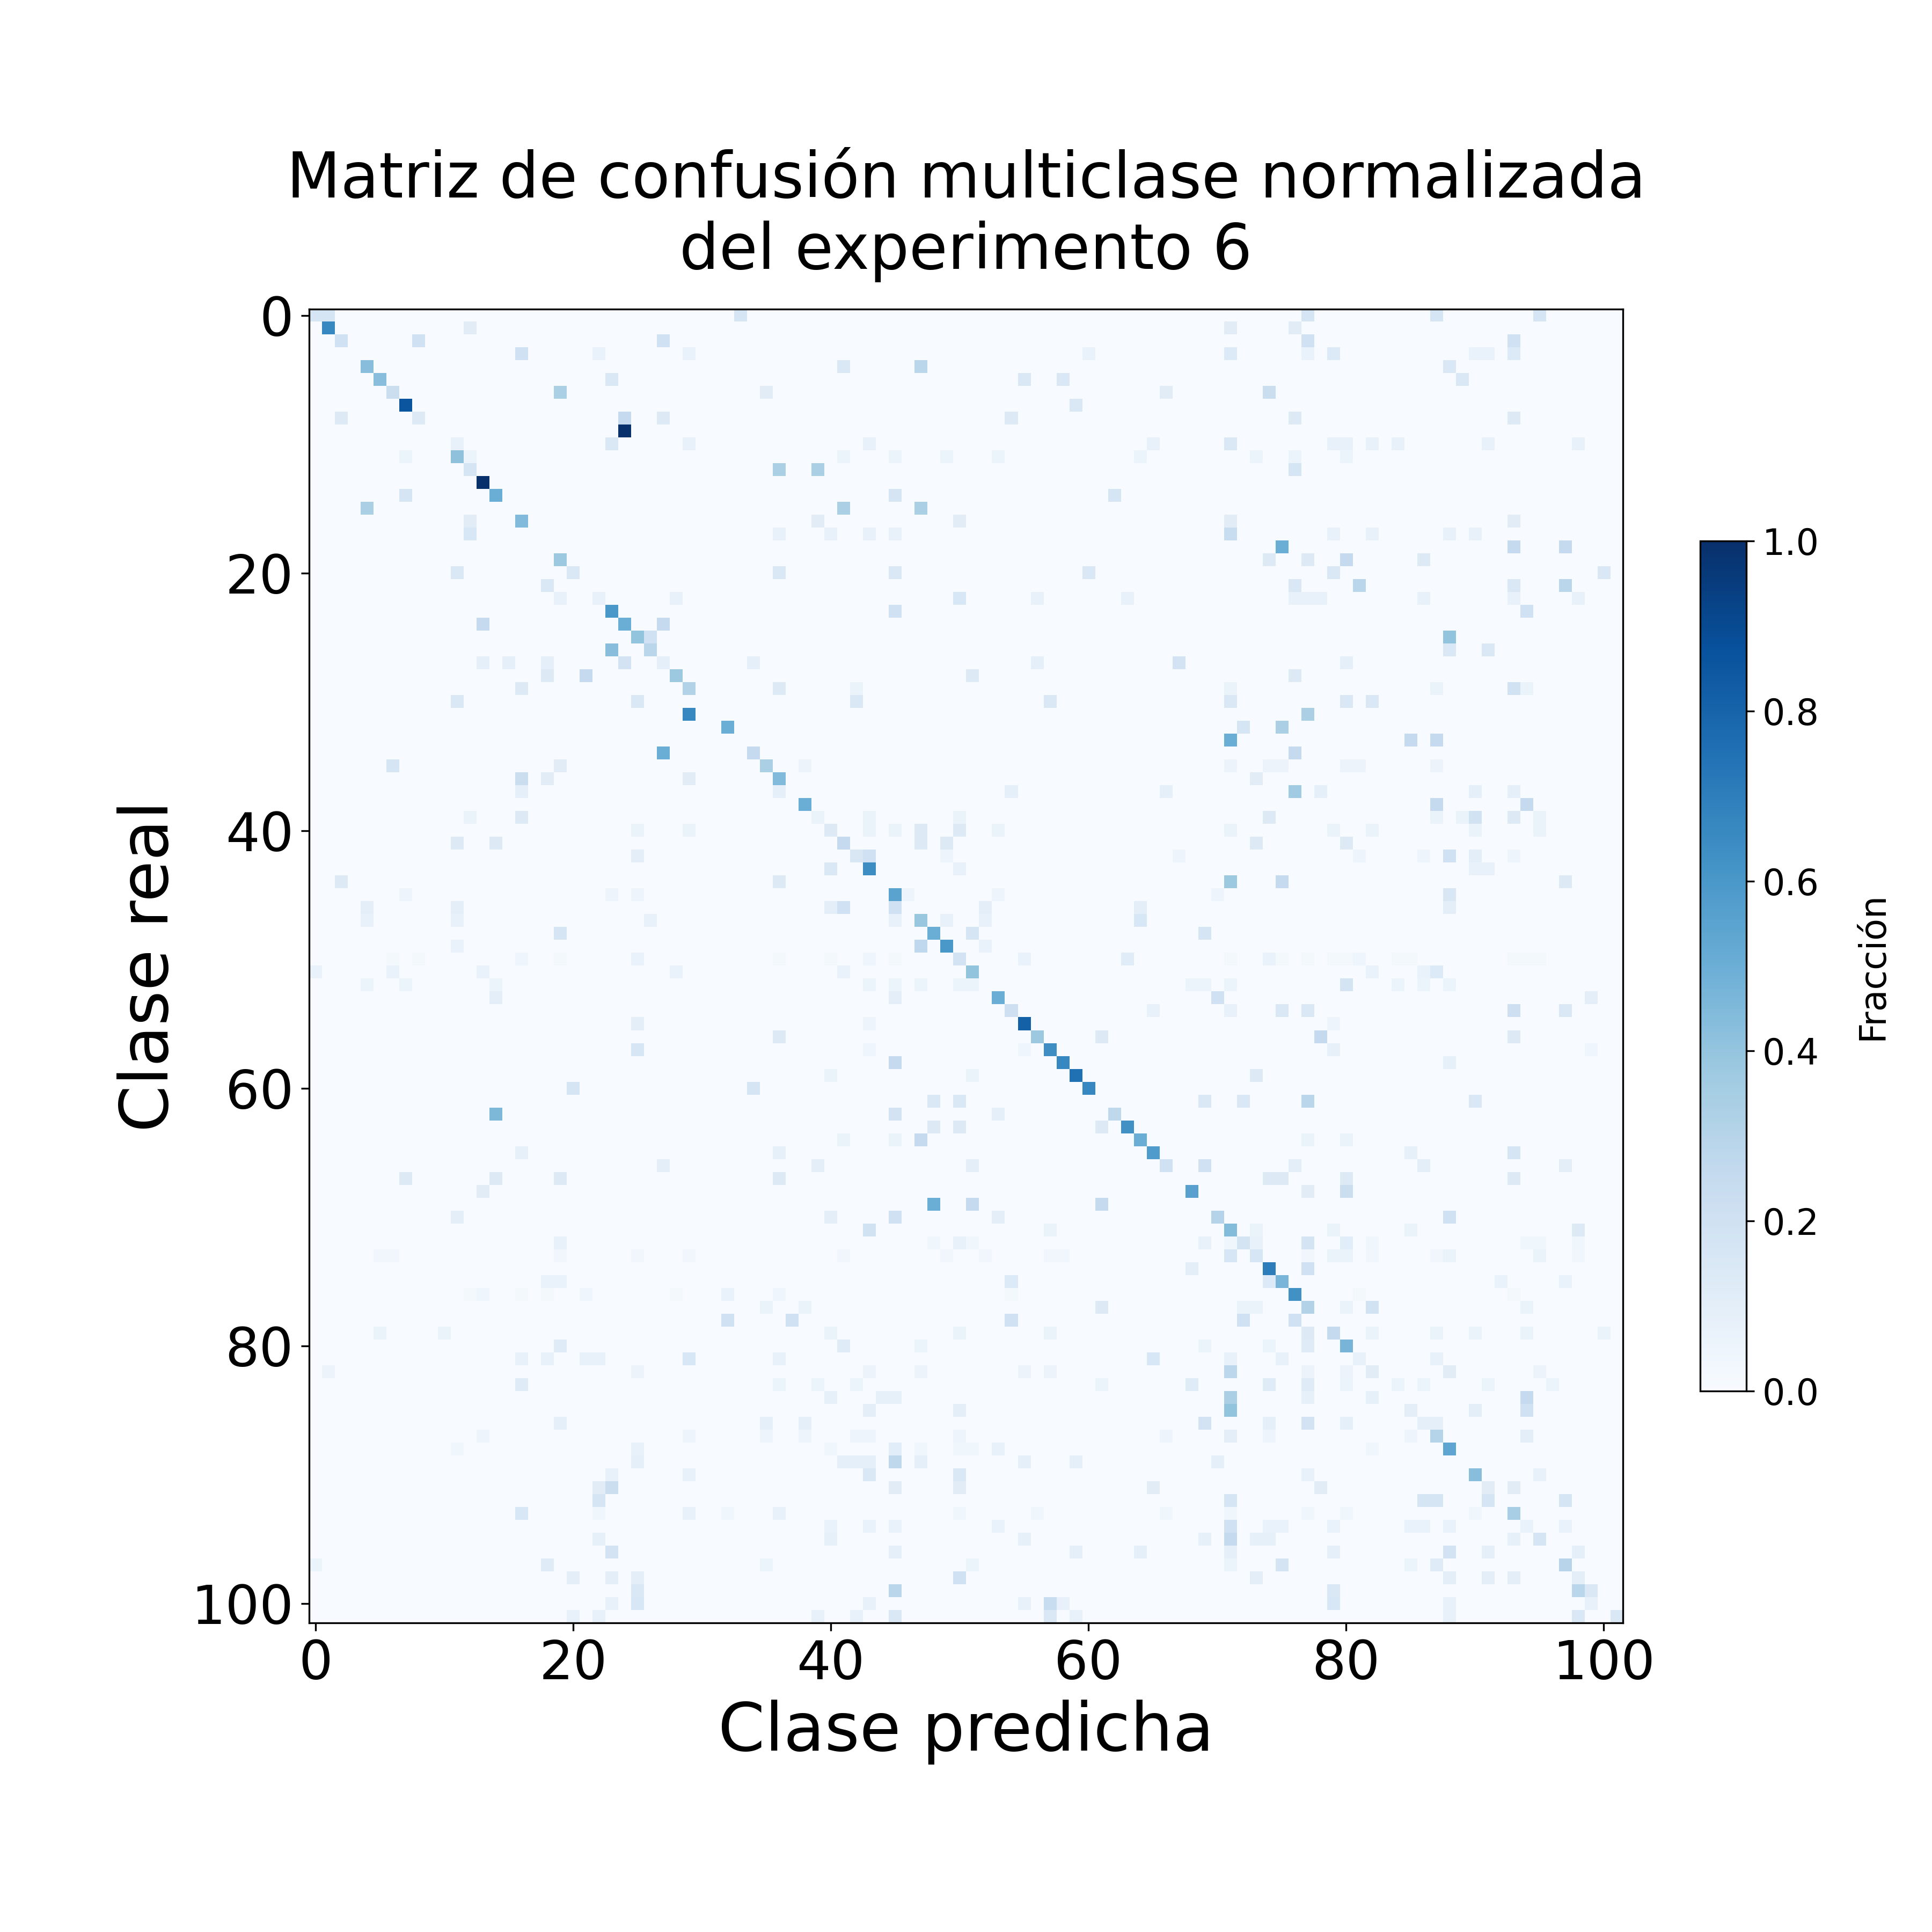
\includegraphics[width=\textwidth]{figures/Experiments_logs/confusion_matrix_04-30-0011.png}
        \caption{}
        \label{fig:confusion_matrix_04-30-0011}
    \end{subfigure}
    \hfill
    \begin{subfigure}{0.45\textwidth}
        \centering
        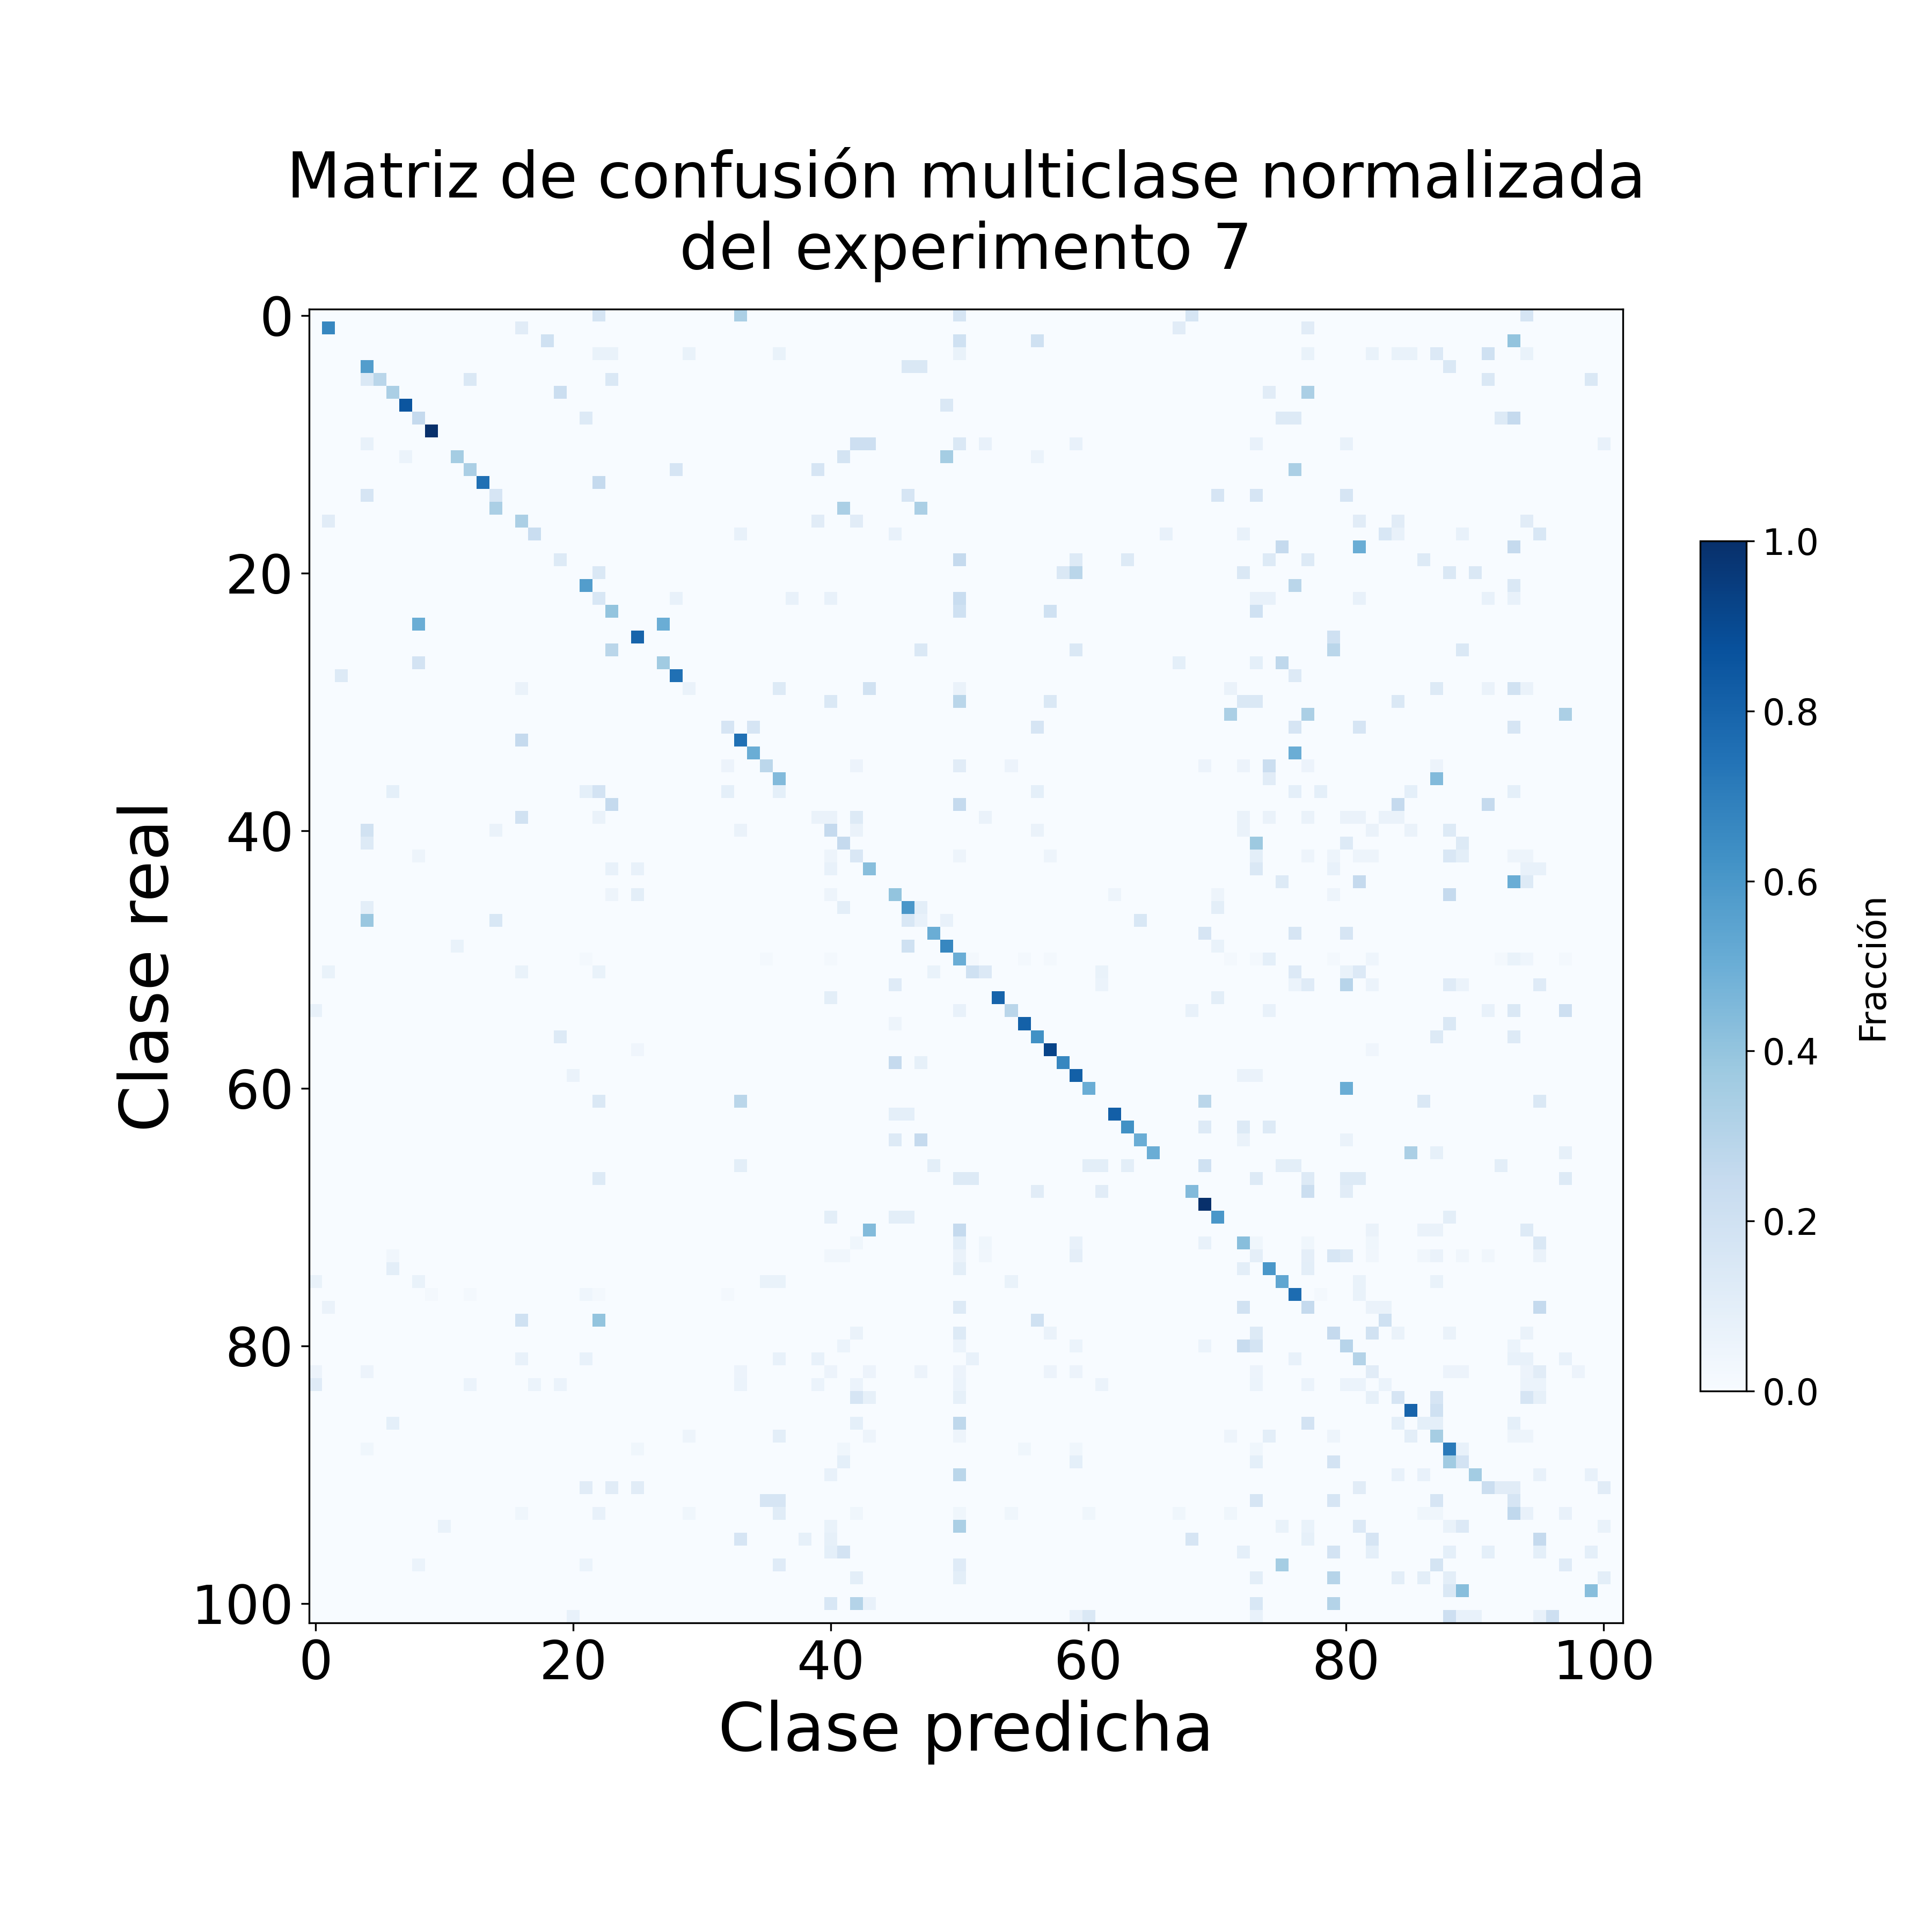
\includegraphics[width=\textwidth]{figures/Experiments_logs/confusion_matrix_04-30-0021.png}
        \caption{}
        \label{fig:confusion_matrix_04-30-0021}
    \end{subfigure}

    \caption{Matrices de confusión multiclase en Flowers102 tras AIM y \textit{data augmentation}.}
    \label{fig:confusion_matrix_04-30-0011-0021}
\end{figure}

En una matriz de confusión ideal se vería casi todo concentrado en la diagonal. En este caso la diagonal ya aparece, lo cual significa que el modelo no está prediciendo completamente al azar, pero sigue habiendo muchos valores fuera de ella. Esto llevó a la tercera hipótesis.

\subsection{Hipótesis 3}

La tercera hipótesis fue que el problema ya no era solo que el modelo no aprendiera, sino que Flowers102 era un dataset difícil para esta fase del proyecto. Tiene 102 clases de flores, muchas de ellas visualmente muy parecidas. Incluso para una persona puede ser complicado distinguir correctamente todas las clases sin un conocimiento previo sobre botánica.

Además, Flowers102 nunca fue el objetivo central del TFG. El objetivo era trabajar con imágenes de material de laboratorio, usando ChemEq25. Por tanto, una vez comprobado que el pipeline funcionaba y que AIM mejoraba el comportamiento, el siguiente paso natural fue cambiar al dataset principal.

\section{Cambio de dataset a ChemEq25}

Antes de implementar cualquier dataset en un modelo, es muy importante revisarlo detenidamente. La parte de limpiar y adaptar los datos es una de las más importantes dentro del \textit{machine learning}, porque si los datos no están bien preparados, es muy difícil obtener buenos resultados después.

Revisando ChemEq25 apareció una particularidad importante. Muchas imágenes tenían dimensiones de $640\times640$ píxeles, pero podían contener más de un objeto de laboratorio. Incluso había fotografías con muchos objetos distintos en la misma escena. Si se introdujera una imagen completa en el clasificador, el modelo no sabría qué objeto debe clasificar. Por eso fue necesario usar las anotaciones YOLO del dataset.

Las anotaciones YOLO indican dónde está cada objeto dentro de la imagen. Con ellas se generaron recortes que contienen un único objeto, y cada recorte mantiene su etiqueta correspondiente.

\begin{figure}[H]
    \centering

    \begin{subfigure}{0.45\textwidth}
        \centering
        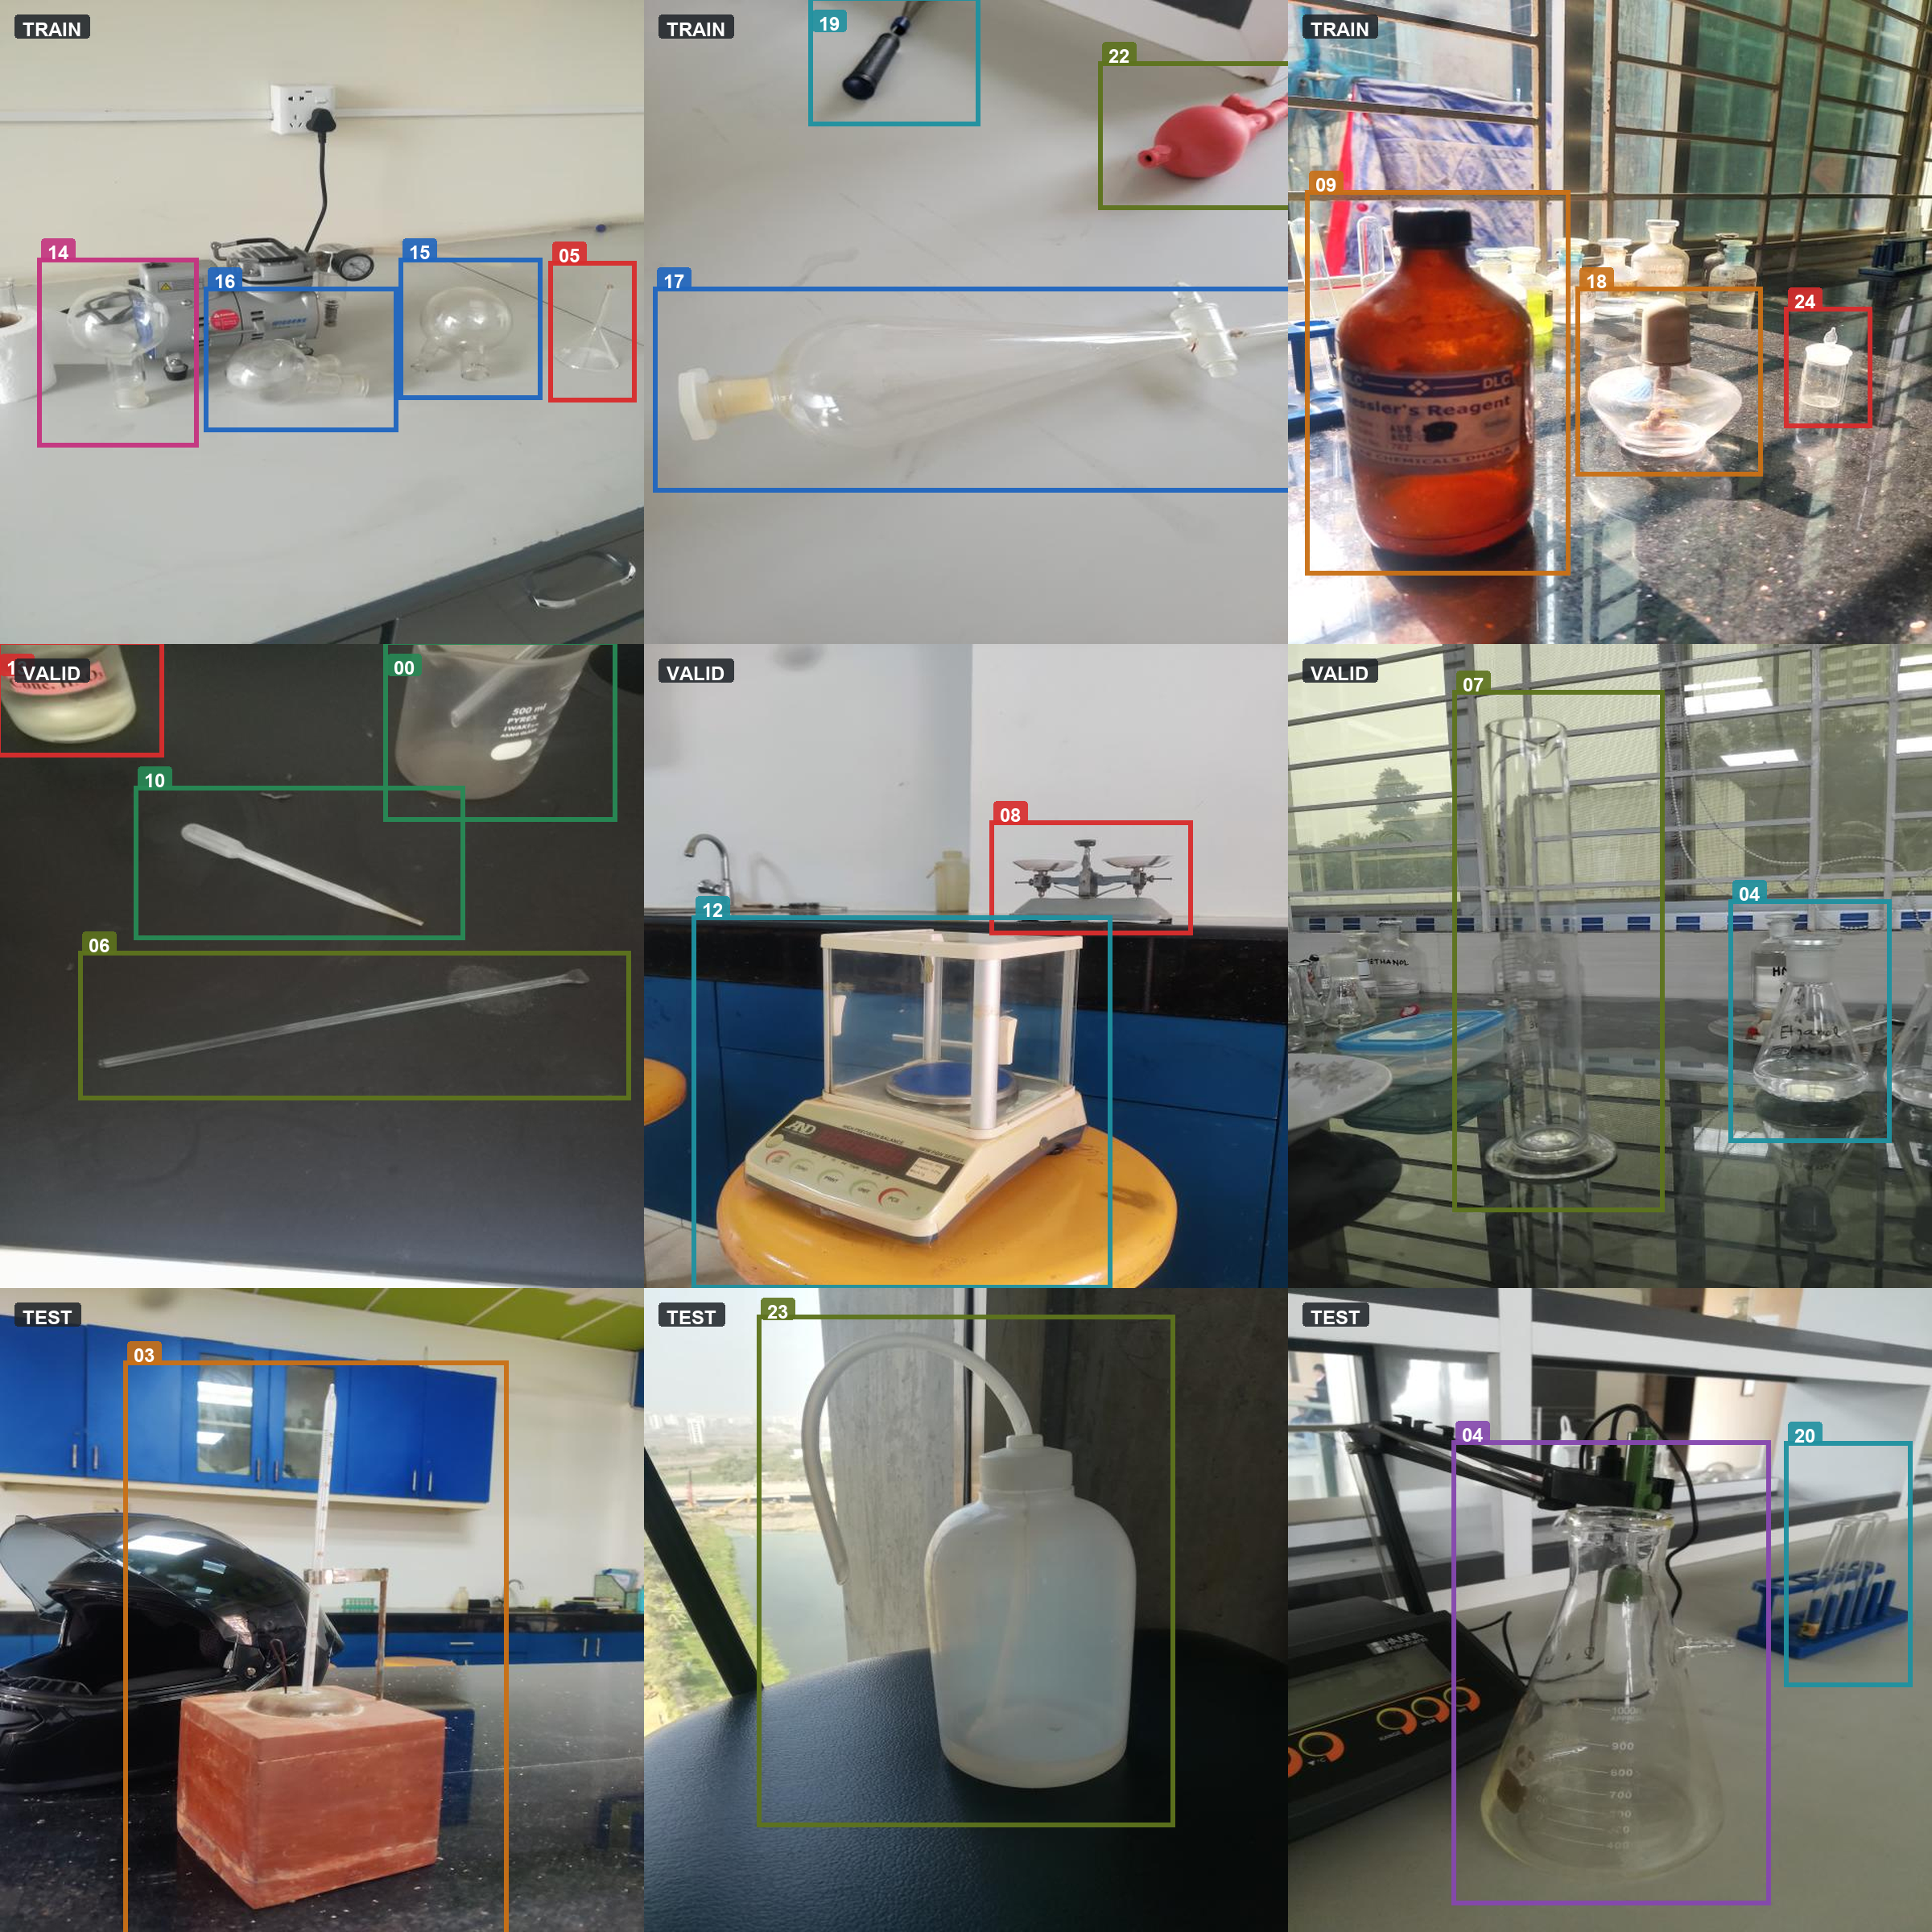
\includegraphics[width=\textwidth]{figures/tfg_dataset_yolo_boxes_square.png}
        \caption{}
        \label{fig:YOLO}
    \end{subfigure}
    \hfill
    \begin{subfigure}{0.45\textwidth}
        \centering
        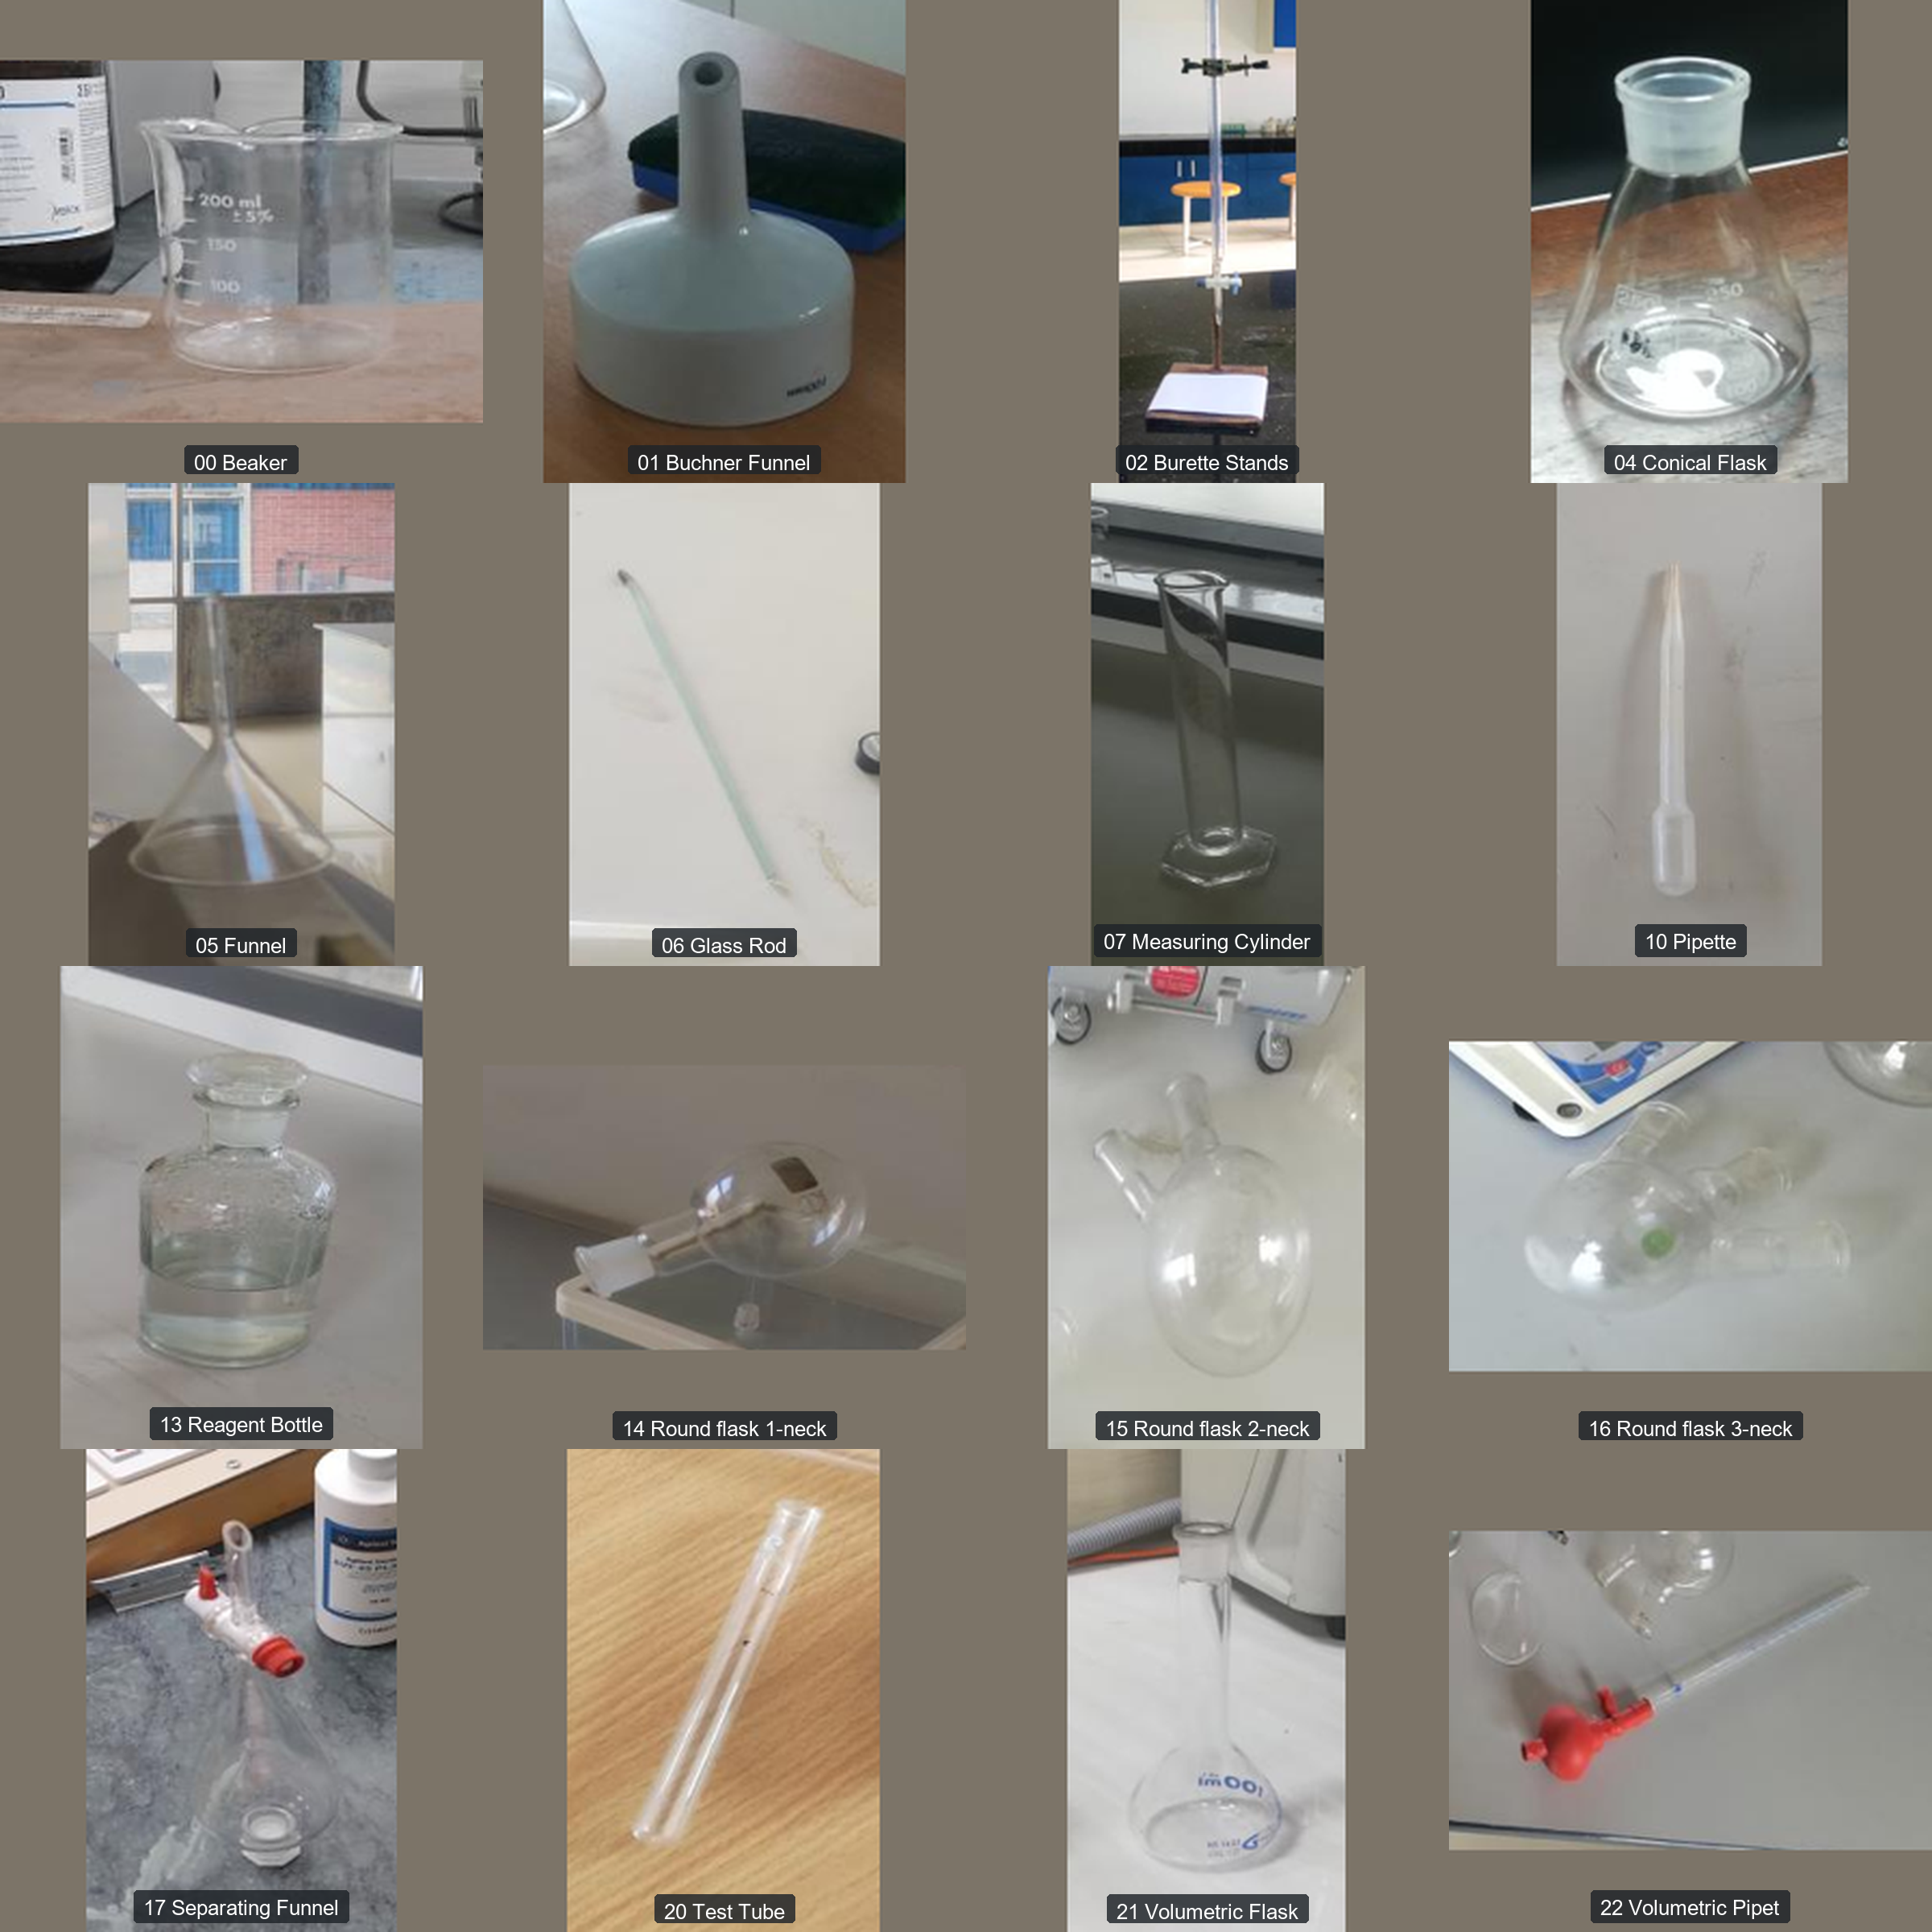
\includegraphics[width=\textwidth]{figures/tfg_dataset_classifier_crops_square.png}
        \caption{}
        \label{fig:crops}
    \end{subfigure}

    \caption{En la figura a) vemos ejemplos de cajas obtenidas a partir de las anotaciones YOLO. En la figura b) vemos ejemplos de los recortes utilizados como entrada del clasificador. El color gris que se ven entre las imágenes es el color de relleno cercano a la media de \textit{ImageNet}. Las imágenes en b) son los recortes tal y como las va a ver el modelo.}
    \label{fig:dataset_crops_YOLO}
\end{figure}

Una vez preparado el dataset, se lanzó el primer experimento serio con ChemEq25:

\begin{figure}[H]
    \centering
    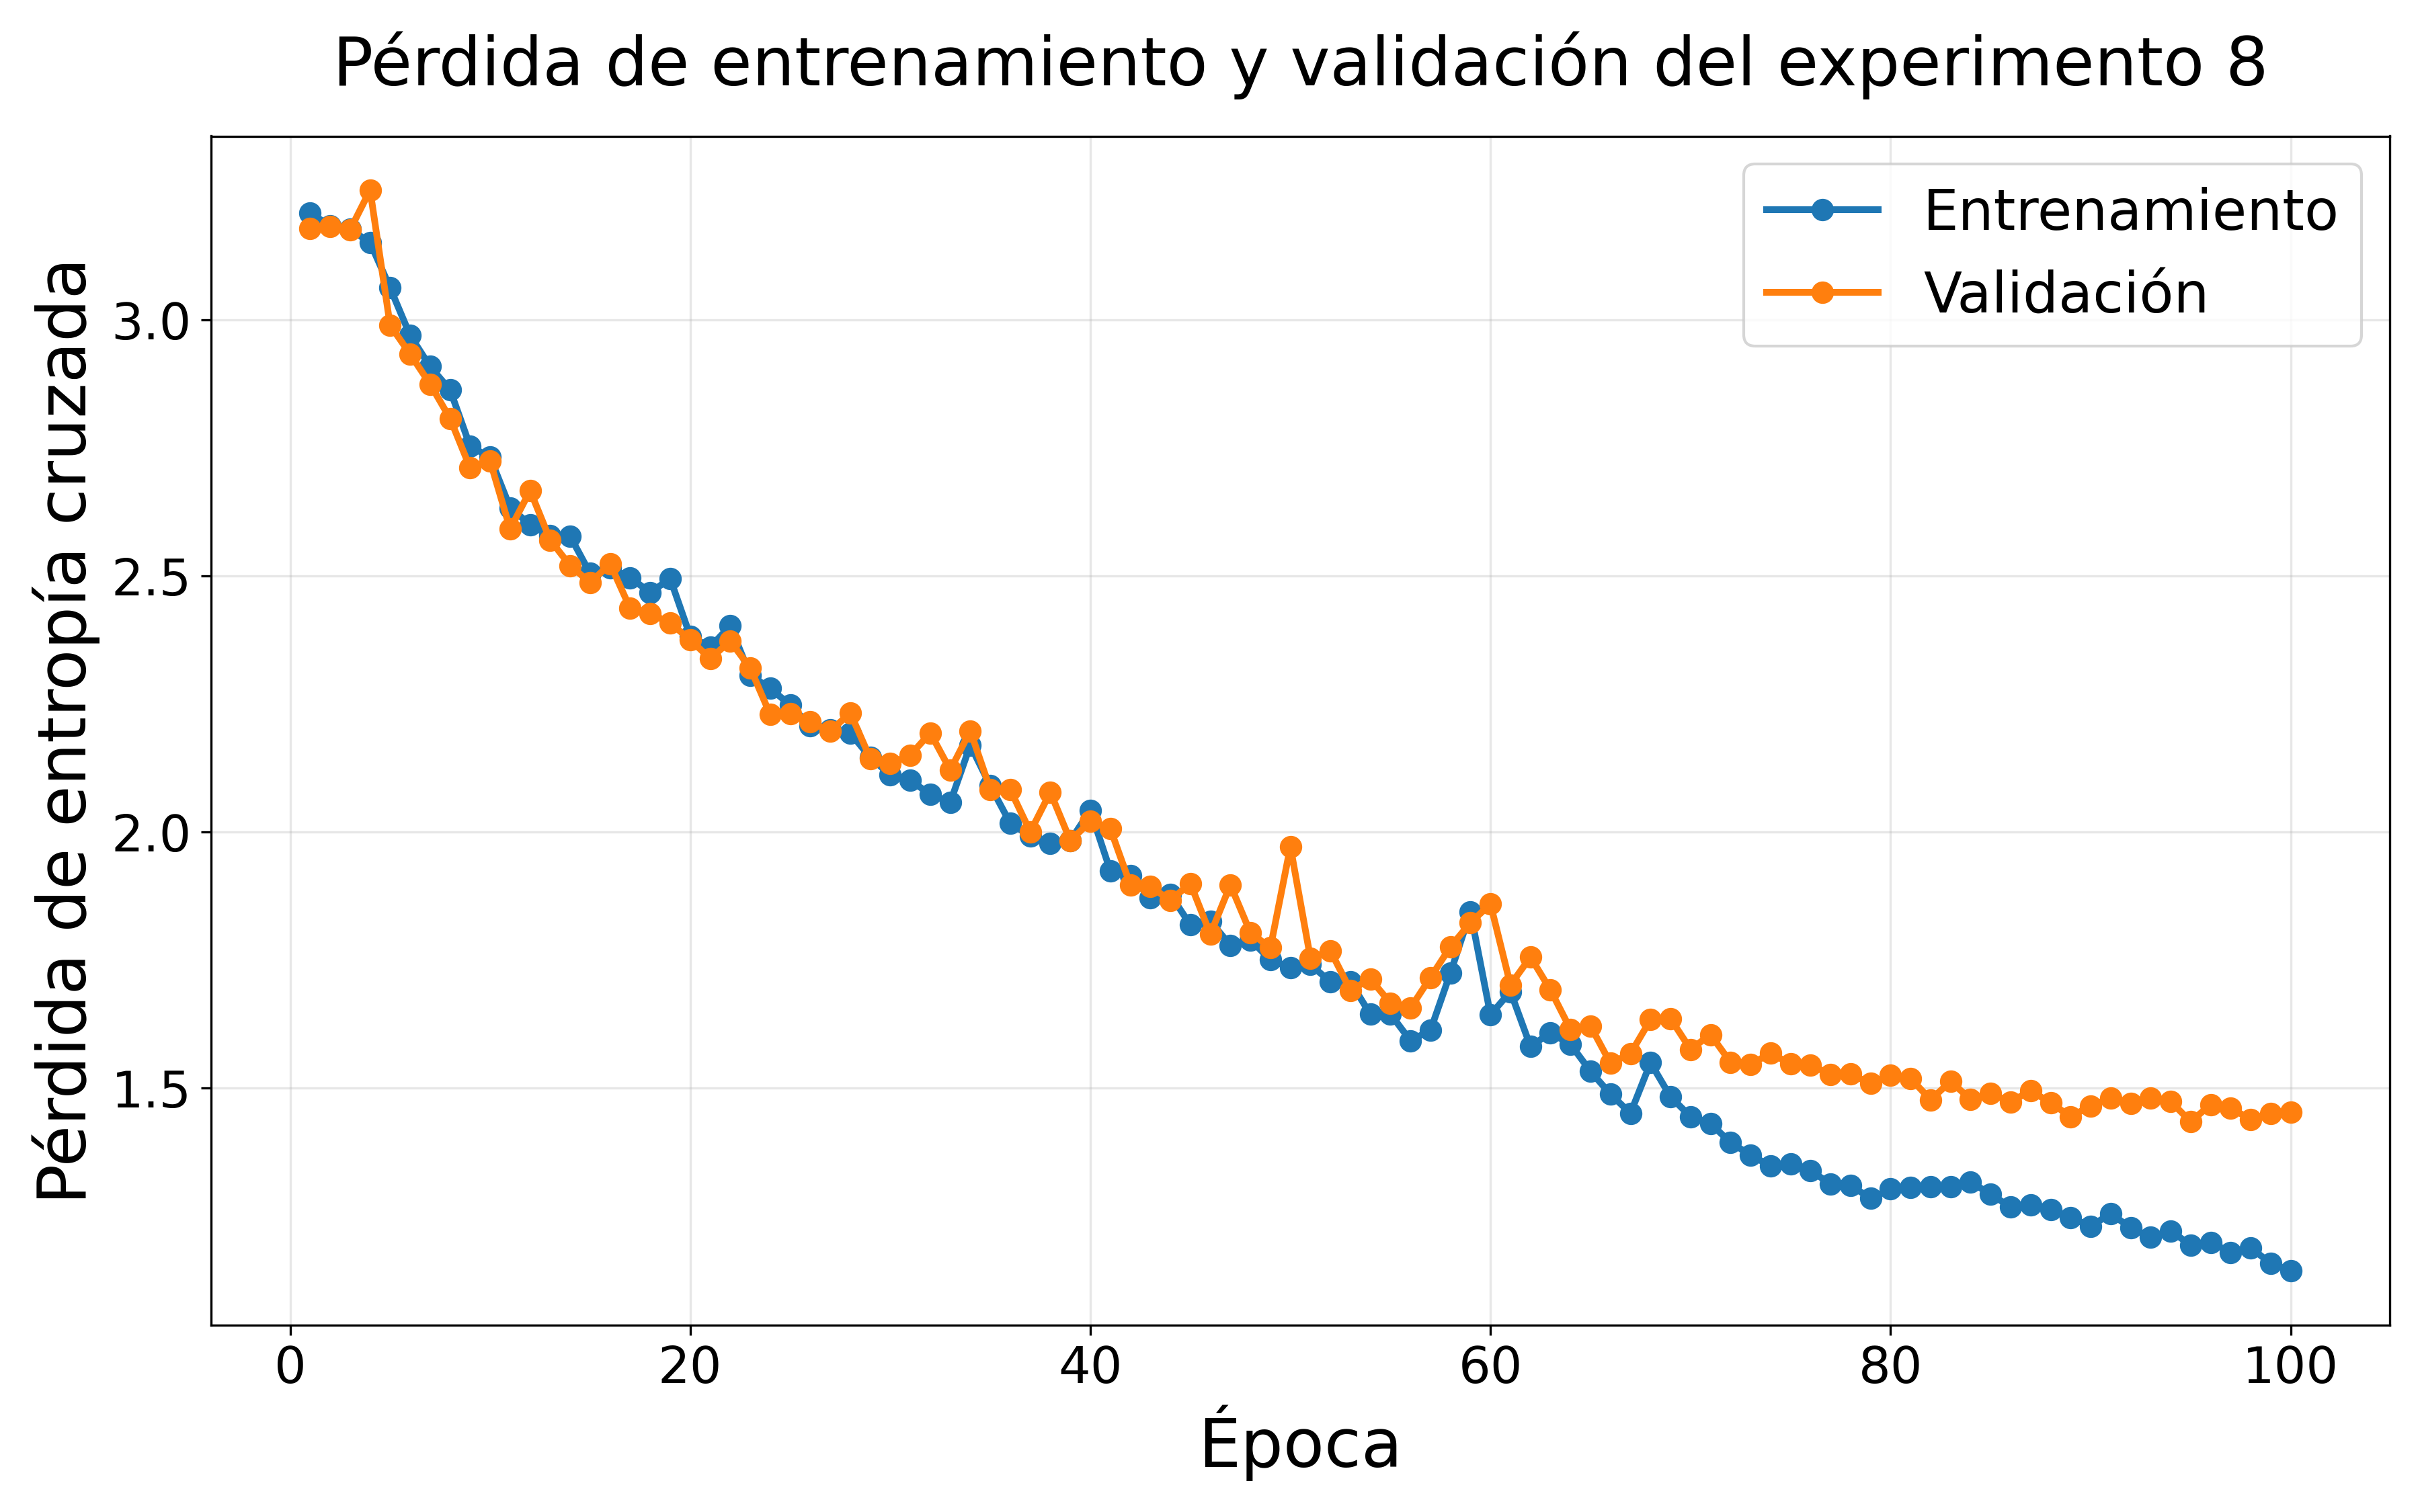
\includegraphics[width=0.55\linewidth]{figures/Experiments_logs/loss_curve_05-05-0953.png}
    \caption{Primer experimento con ChemEq25.}
    \label{fig:loss_curve_05-05-0953}
\end{figure}

\begin{table}[H]
\centering
\small
\begin{tabular}{lccccc}
\toprule
\textbf{Experimento} & \textbf{LR} & \textbf{Acc. eval} & \textbf{Top-5} & \textbf{Eval loss} & \textbf{Acc. final} \\
\midrule
\texttt{8} & 0,0005 & 57,00\% & 86,22\% & 1,4343 & 56,86\% \\
\bottomrule
\end{tabular}
\caption{Primer resultado sobre ChemEq25.}
\label{tab:chemeq_primer_run}
\end{table}

El salto respecto a Flowers102 fue muy grande. La precisión pasó de 33,96\% en Flowers a 57,00\% en ChemEq25, y el top-5 alcanzó 86,22\%. Esto confirmó la hipótesis 3. El problema de Flowers102 no era solo la arquitectura, sino también la dificultad de separar 102 clases de flores muy parecidas. Con 25 clases de material de laboratorio, el modelo empezó a mostrar mucha más capacidad.

\subsection{Efecto del learning rate}

El siguiente cambio fue reducir el \textit{learning rate} de 0,0005 a 0,00025. El \textit{learning rate} es el tamaño del paso que da el optimizador al actualizar los parámetros. Si es demasiado alto, el modelo puede moverse de forma brusca por el espacio de parámetros y no estabilizarse bien. Si es demasiado bajo, el entrenamiento puede avanzar muy lento.

\begin{figure}[H]
    \centering

    \begin{subfigure}{0.45\textwidth}
        \centering
        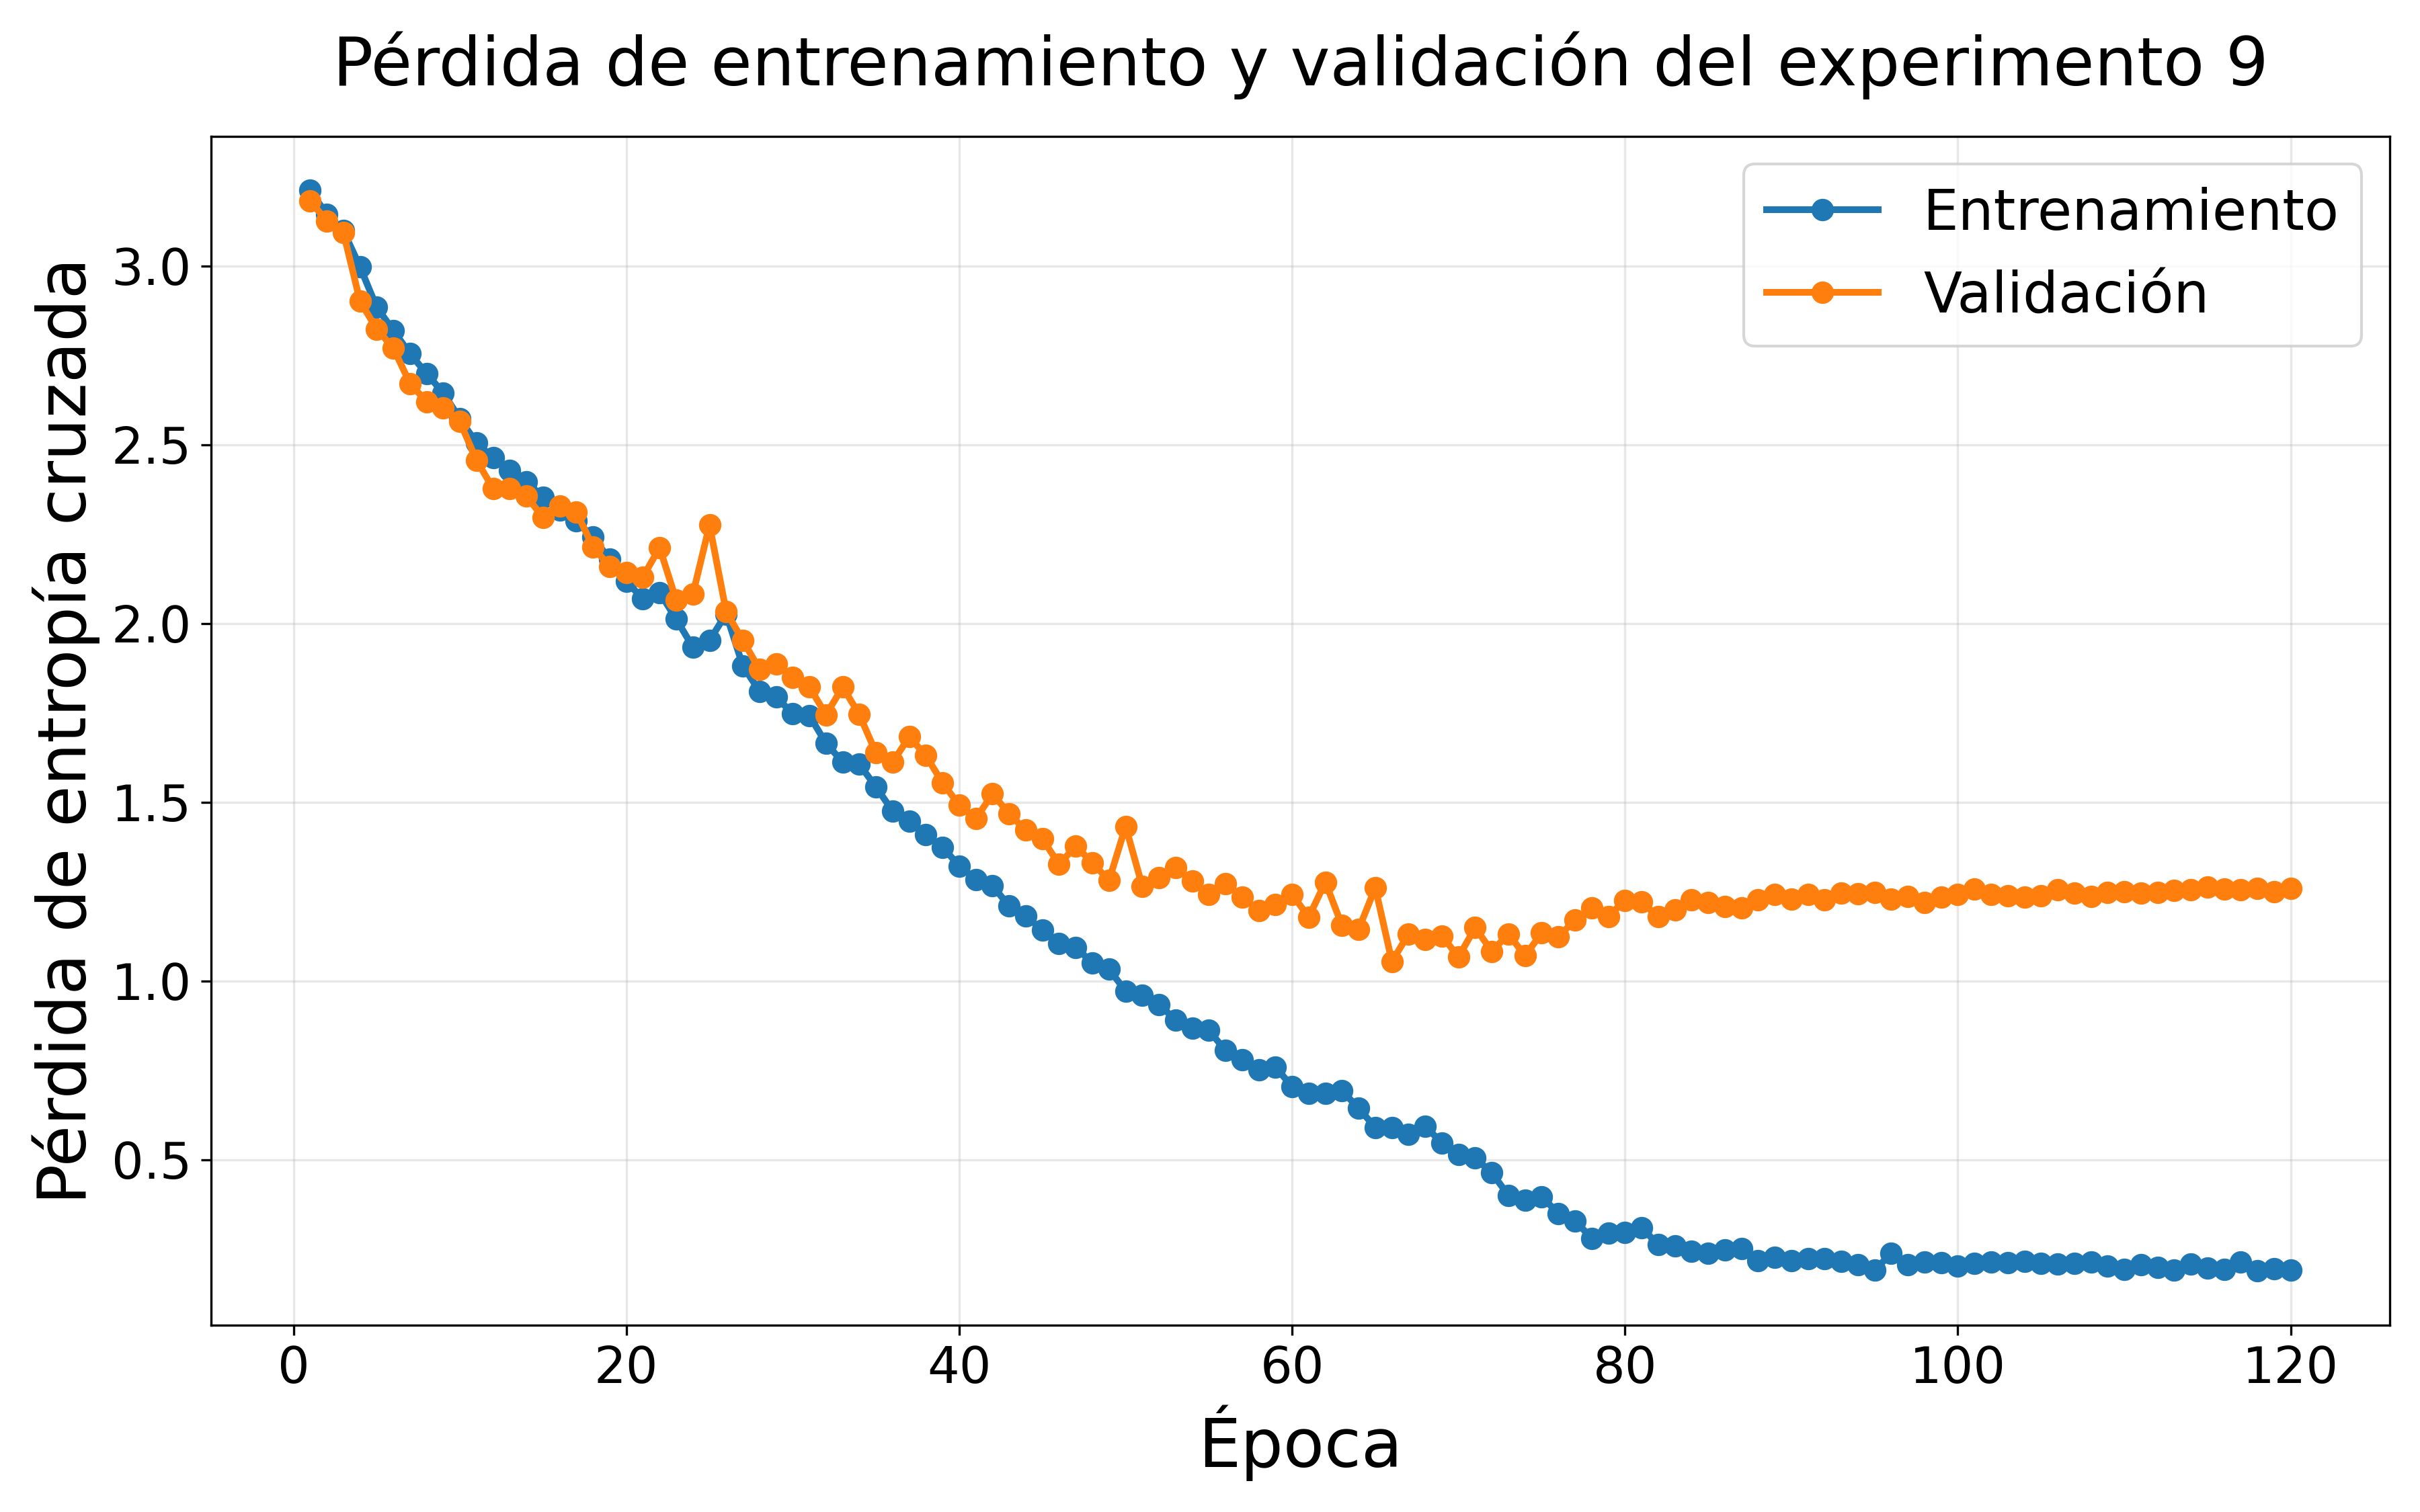
\includegraphics[width=\textwidth]{figures/Experiments_logs/loss_curve_05-05-1119.png}
        \caption{}
        \label{fig:loss_curve_05-05-1119}
    \end{subfigure}
    \hfill
    \begin{subfigure}{0.45\textwidth}
        \centering
        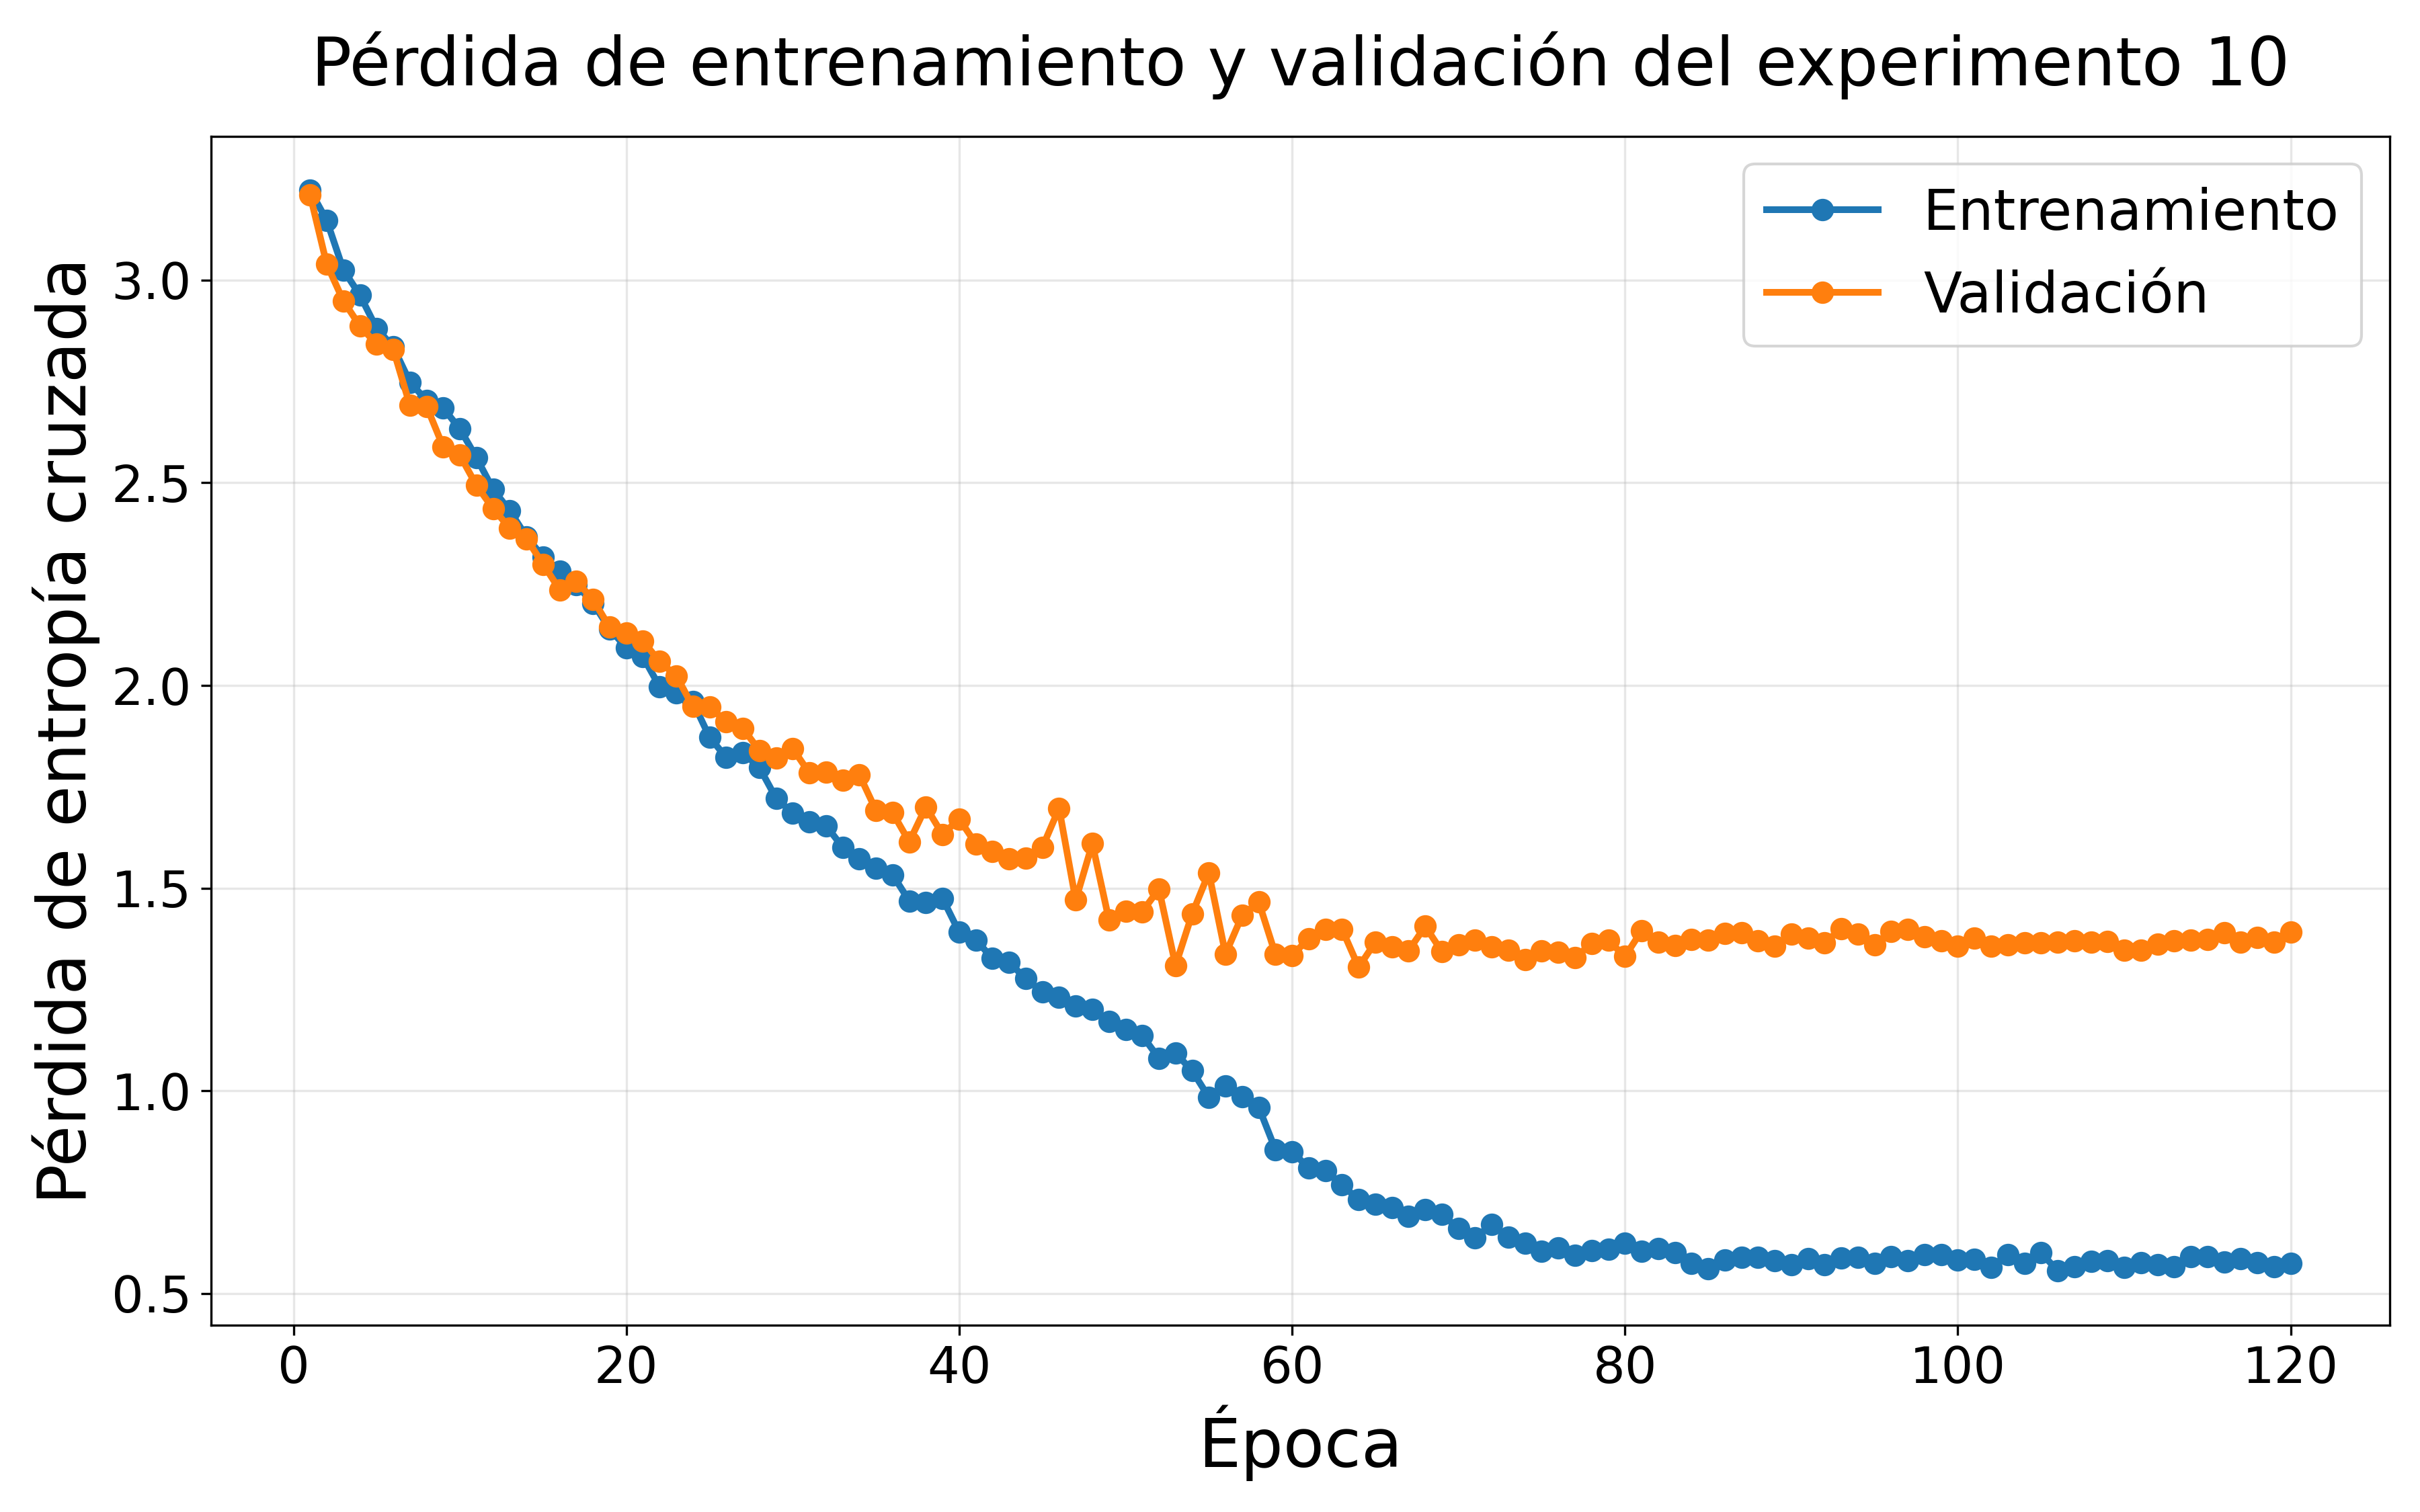
\includegraphics[width=\textwidth]{figures/Experiments_logs/loss_curve_05-05-1145.png}
        \caption{}
        \label{fig:loss_curve_05-05-1145}
    \end{subfigure}

    \caption{Mismo experimento que \figref{fig:loss_curve_05-05-0953}, pero con \textit{learning rate} menor.}
    \label{fig:loss_curve_05-05-1119-1145}
\end{figure}

\begin{table}[H]
\centering
\scriptsize
\begin{tabular}{lcccccc}
\toprule
\textbf{Experimento} & \textbf{Cambio} & \textbf{Acc.} & \textbf{Top-5} & \textbf{Loss} & \textbf{Train final} & \textbf{Eval final} \\
\midrule
\texttt{8} & LR 0,0005 & 57,00\% & 86,22\% & 1,4343 & 64,80\% & 56,86\% \\
\texttt{9} & LR 0,00025 & 75,23\% & 93,90\% & 1,0539 & 94,78\% & 74,66\% \\
\texttt{10} & MLP head & 70,57\% & 94,33\% & 1,3047 & 80,34\% & 69,56\% \\
\bottomrule
\end{tabular}
\caption{Comparación de los primeros ajustes sobre ChemEq25.}
\label{tab:chemeq_lr_head}
\end{table}

La bajada del \textit{learning rate} produjo una mejora muy fuerte: de 57,00\% a 75,23\%. Esto no significa que el modelo empezara desde un punto distinto, porque la \textit{seed} era la misma. Lo que cambió fue la trayectoria de optimización. Con pasos más pequeños, el modelo encontró una zona mucho mejor.

También se probó una cabeza MLP en vez de una cabeza lineal. La motivación era que el top-5 era alto, así que quizá la representación final contenía información suficiente, pero faltaba una separación más fina entre clases. Sin embargo, la MLP no mejoró el resultado, se quedó en 70,57\%. Por eso se mantuvo la cabeza lineal como opción principal.

En el experiemento con \textit{learning rate} 0,00025 apareció otro patrón interesante. La mejor \textit{eval loss} se alcanzó en la época 66, pero la mejor precisión llegó en la época 104. Esto indica que el modelo acertaba más ejemplos, pero cuando fallaba podía hacerlo con más confianza. Esa lectura motivó los siguientes cambios, \textit{warmup}, regularización y \textit{label smoothing}.

\section{Ajustes de entrenamiento y regularización}

A partir de este punto hubo muchos experimentos. Por cada experimento que se hacía, se iban atacando los problemas observados. Optimización inestable, sobreconfianza, clases parecidas y sensibilidad a la seed.

\begin{figure}[htbp]
    \centering

    \begin{subfigure}{0.45\textwidth}
        \centering
        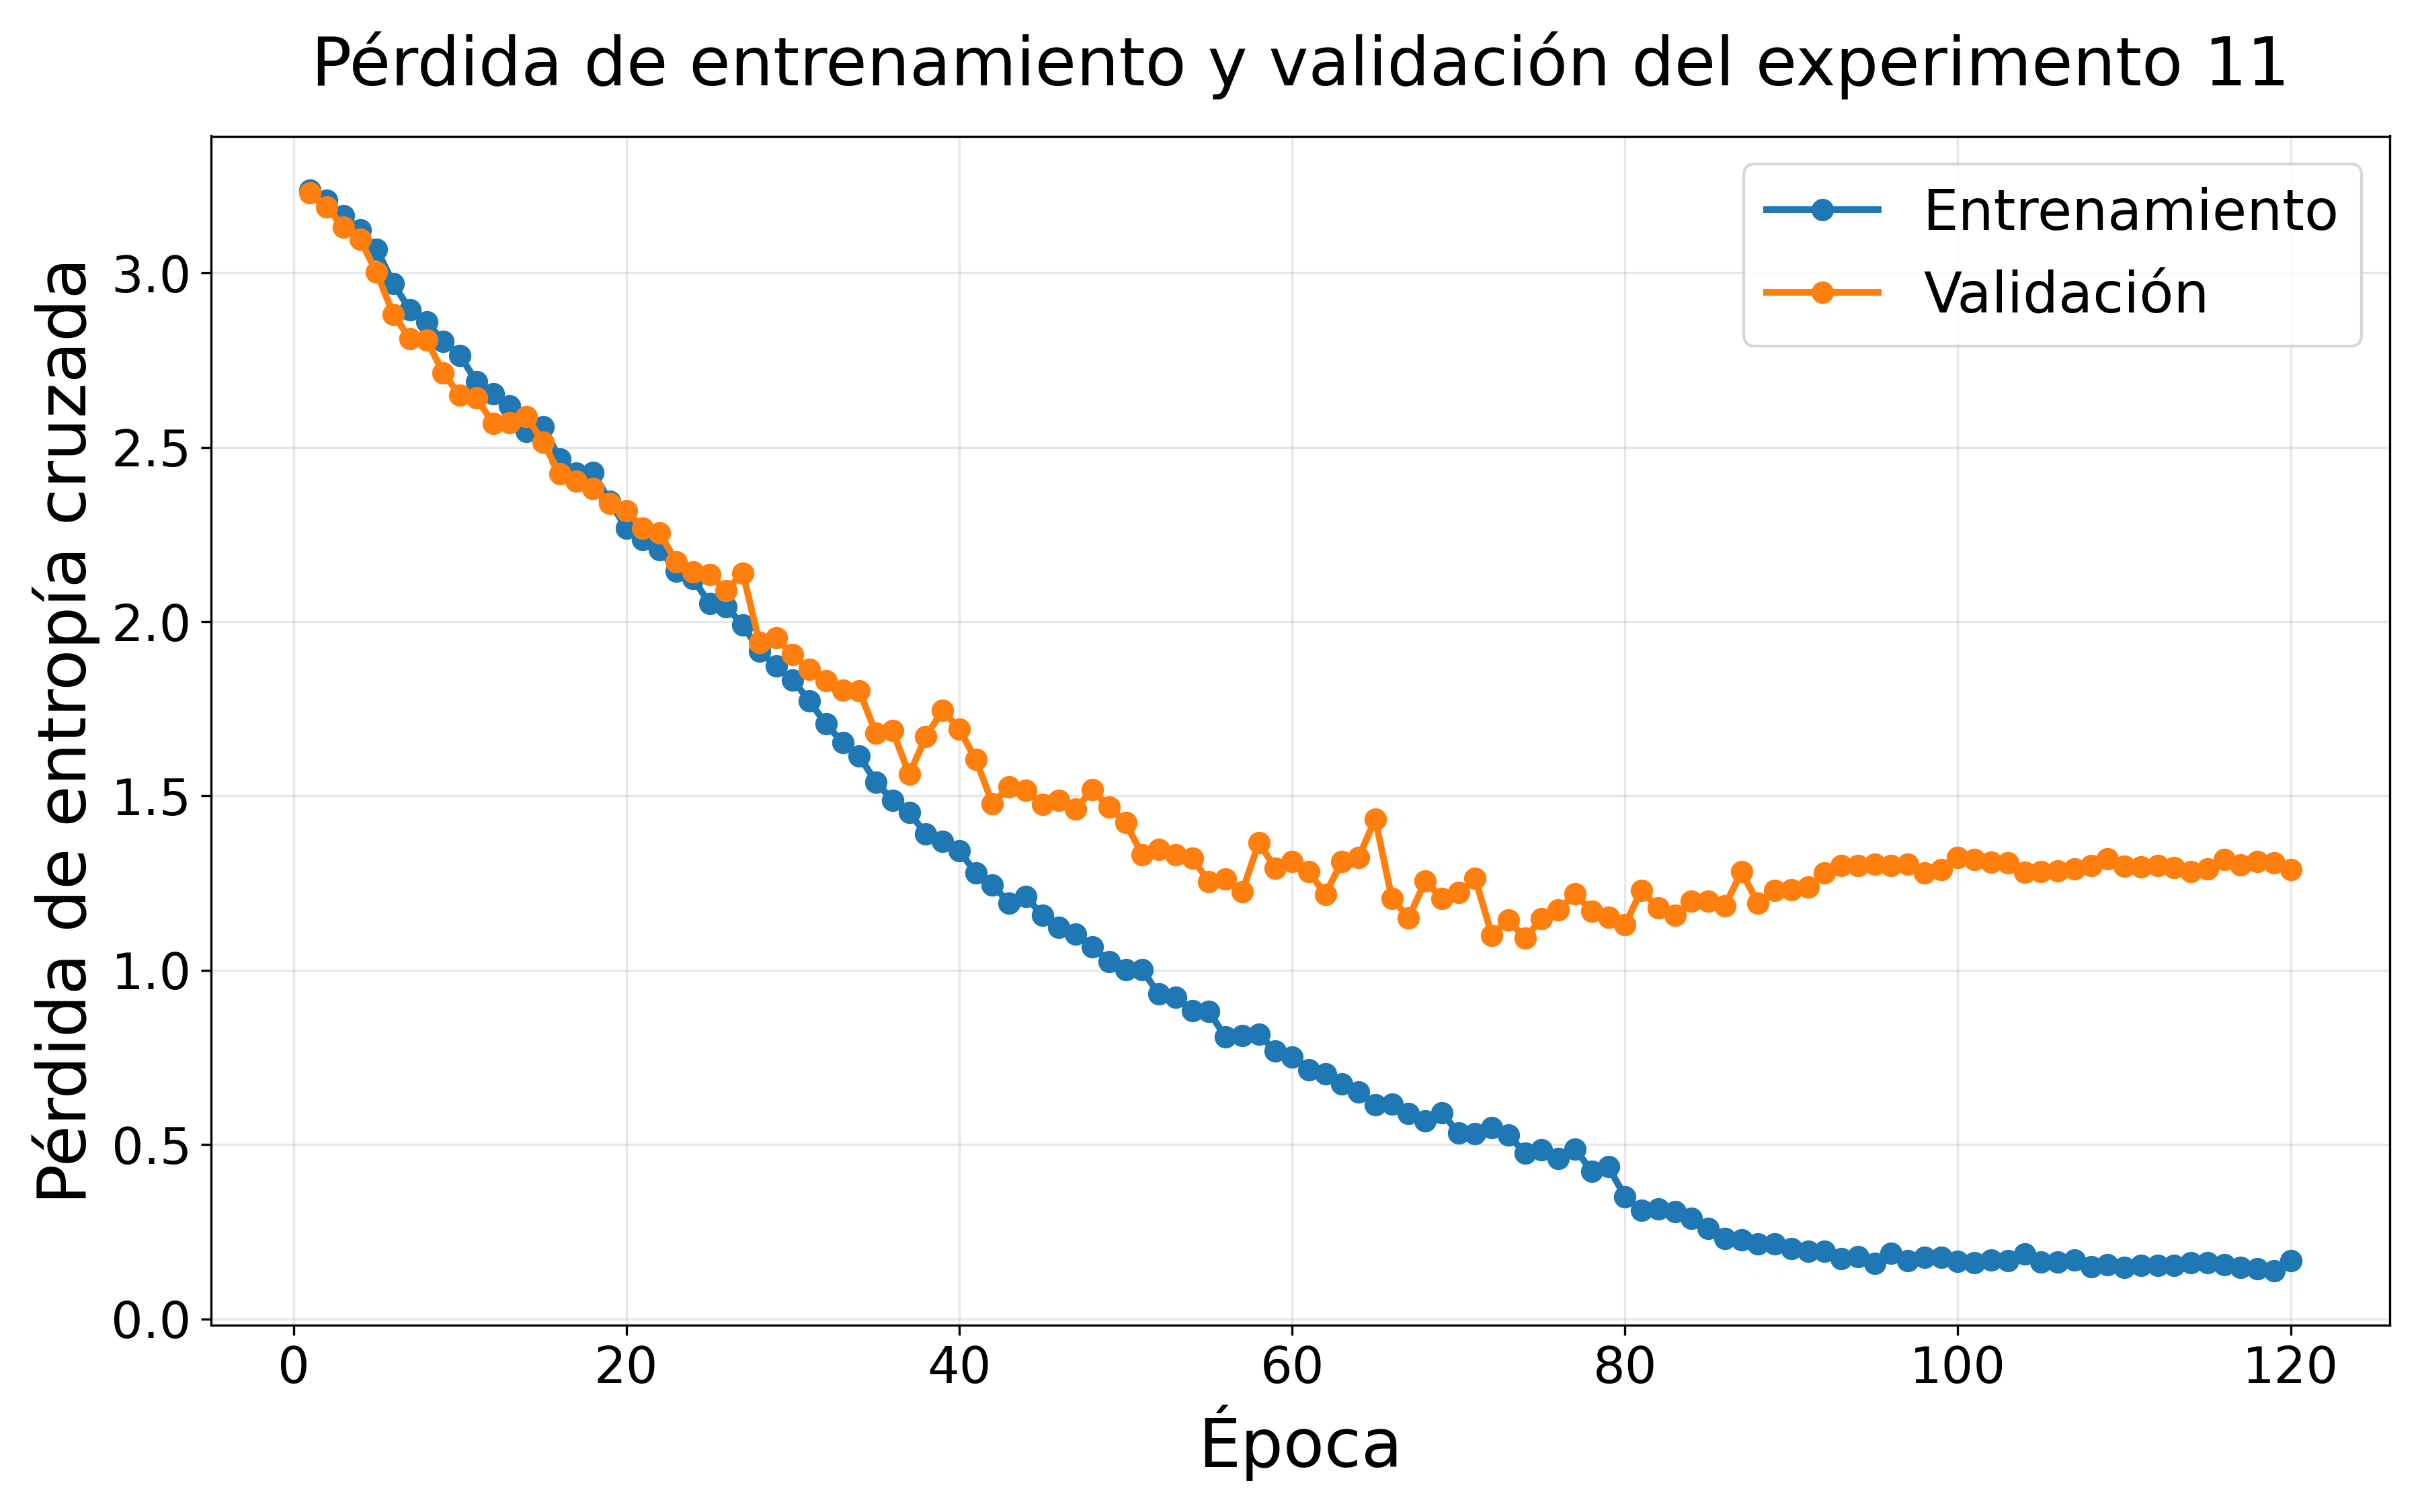
\includegraphics[width=\textwidth]{figures/Experiments_logs/loss_curve_05-07-0857.png}
        \caption{}
        \label{fig:loss_curve_05-07-0857}
    \end{subfigure}
    \hfill
    \begin{subfigure}{0.45\textwidth}
        \centering
        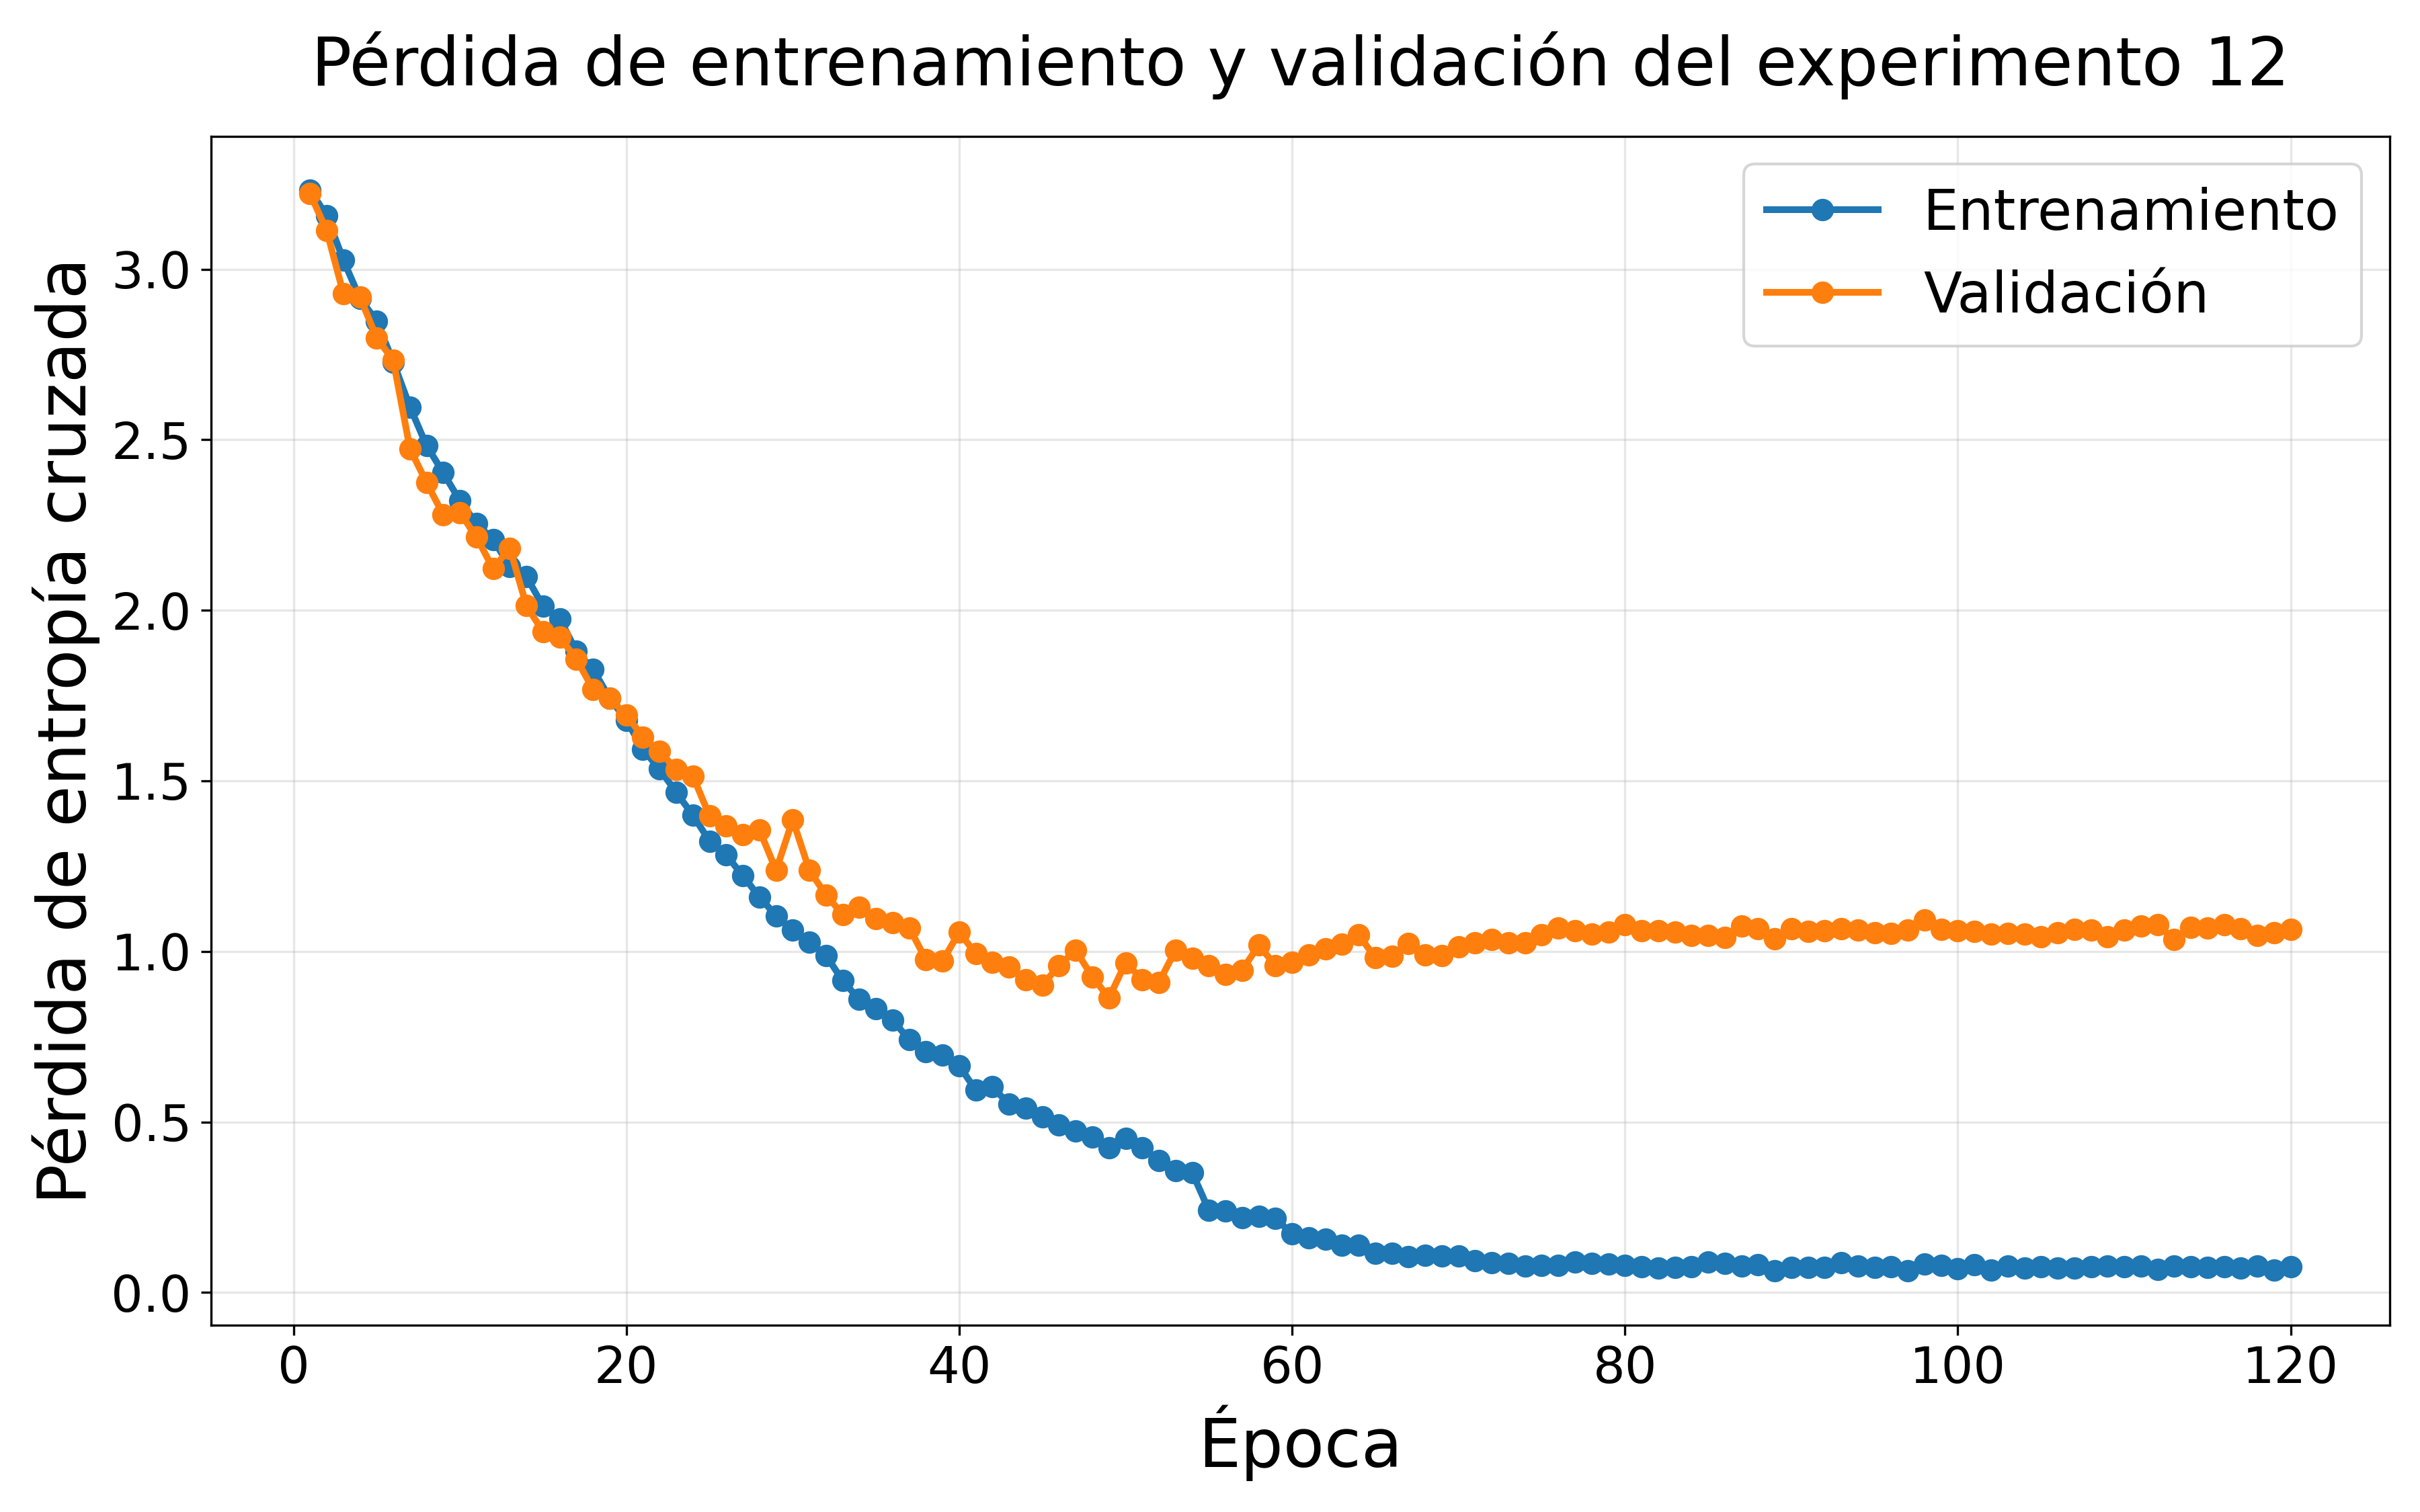
\includegraphics[width=\textwidth]{figures/Experiments_logs/loss_curve_05-07-1304.png}
        \caption{}
        \label{fig:loss_curve_05-07-1304}
    \end{subfigure}

    \vspace{0.4cm}

    \begin{subfigure}{0.45\textwidth}
        \centering
        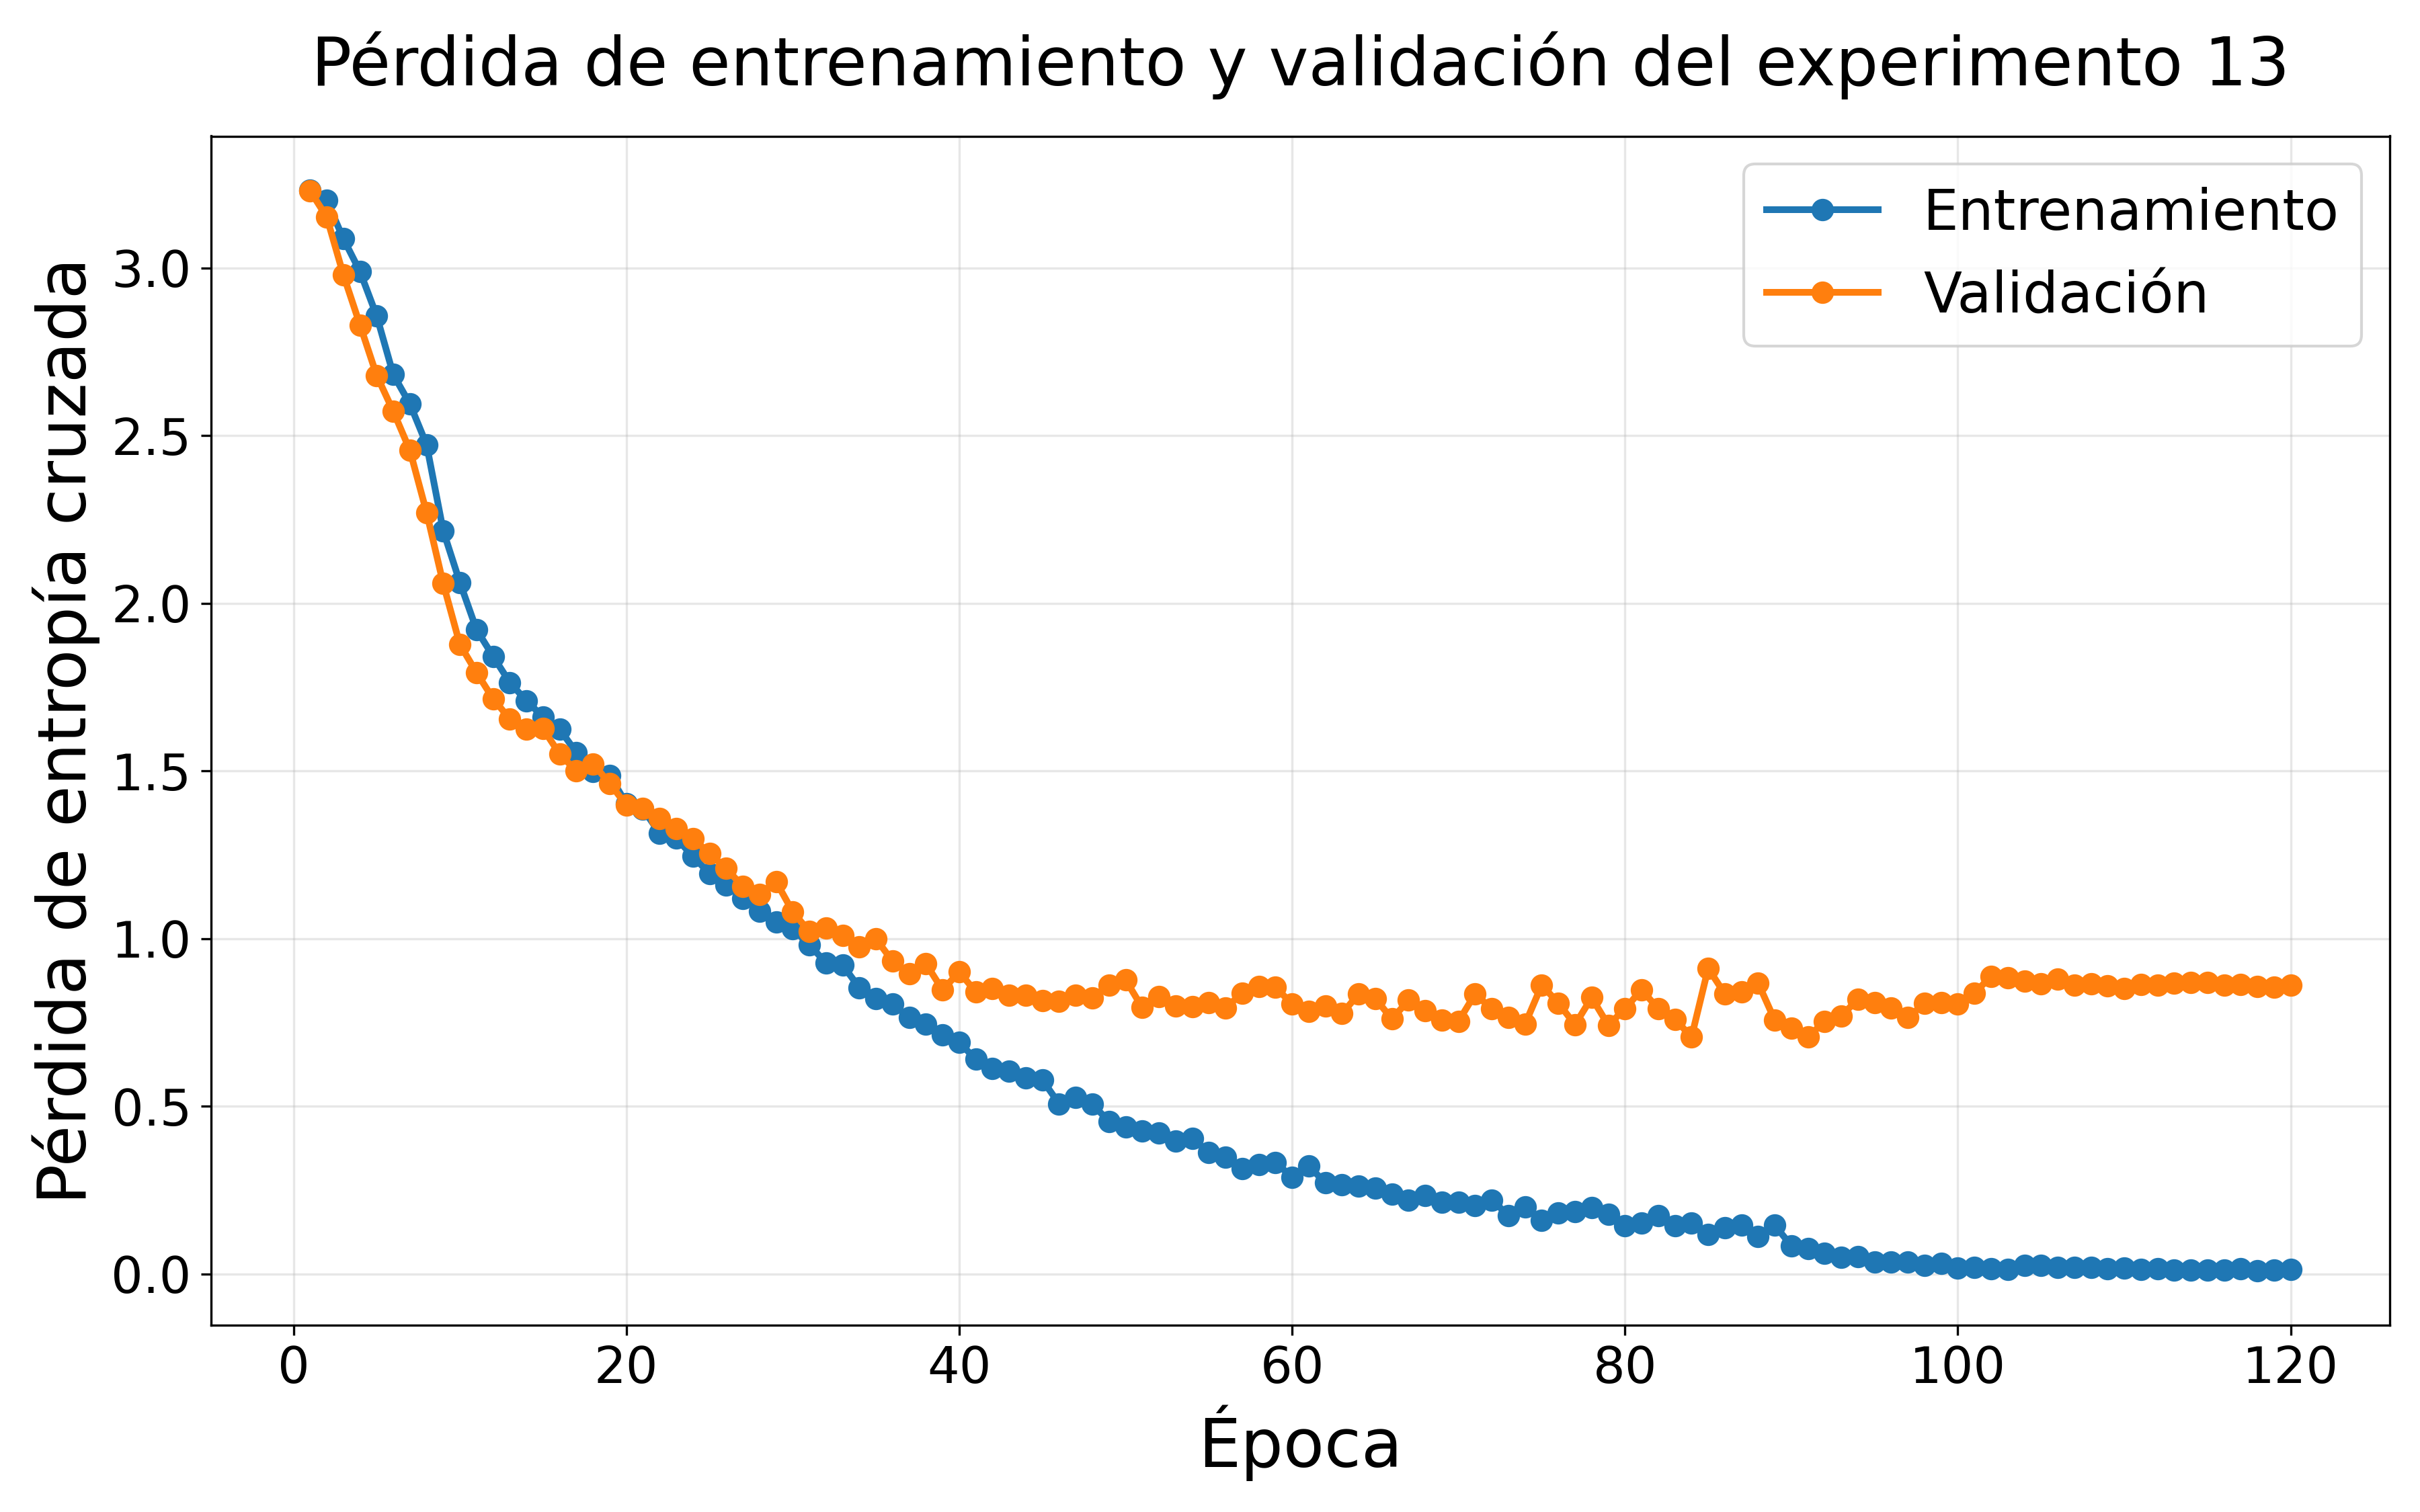
\includegraphics[width=\textwidth]{figures/Experiments_logs/loss_curve_05-08-1400.png}
        \caption{}
        \label{fig:loss_curve_05-08-1400}
    \end{subfigure}
    \hfill
    \begin{subfigure}{0.45\textwidth}
        \centering
        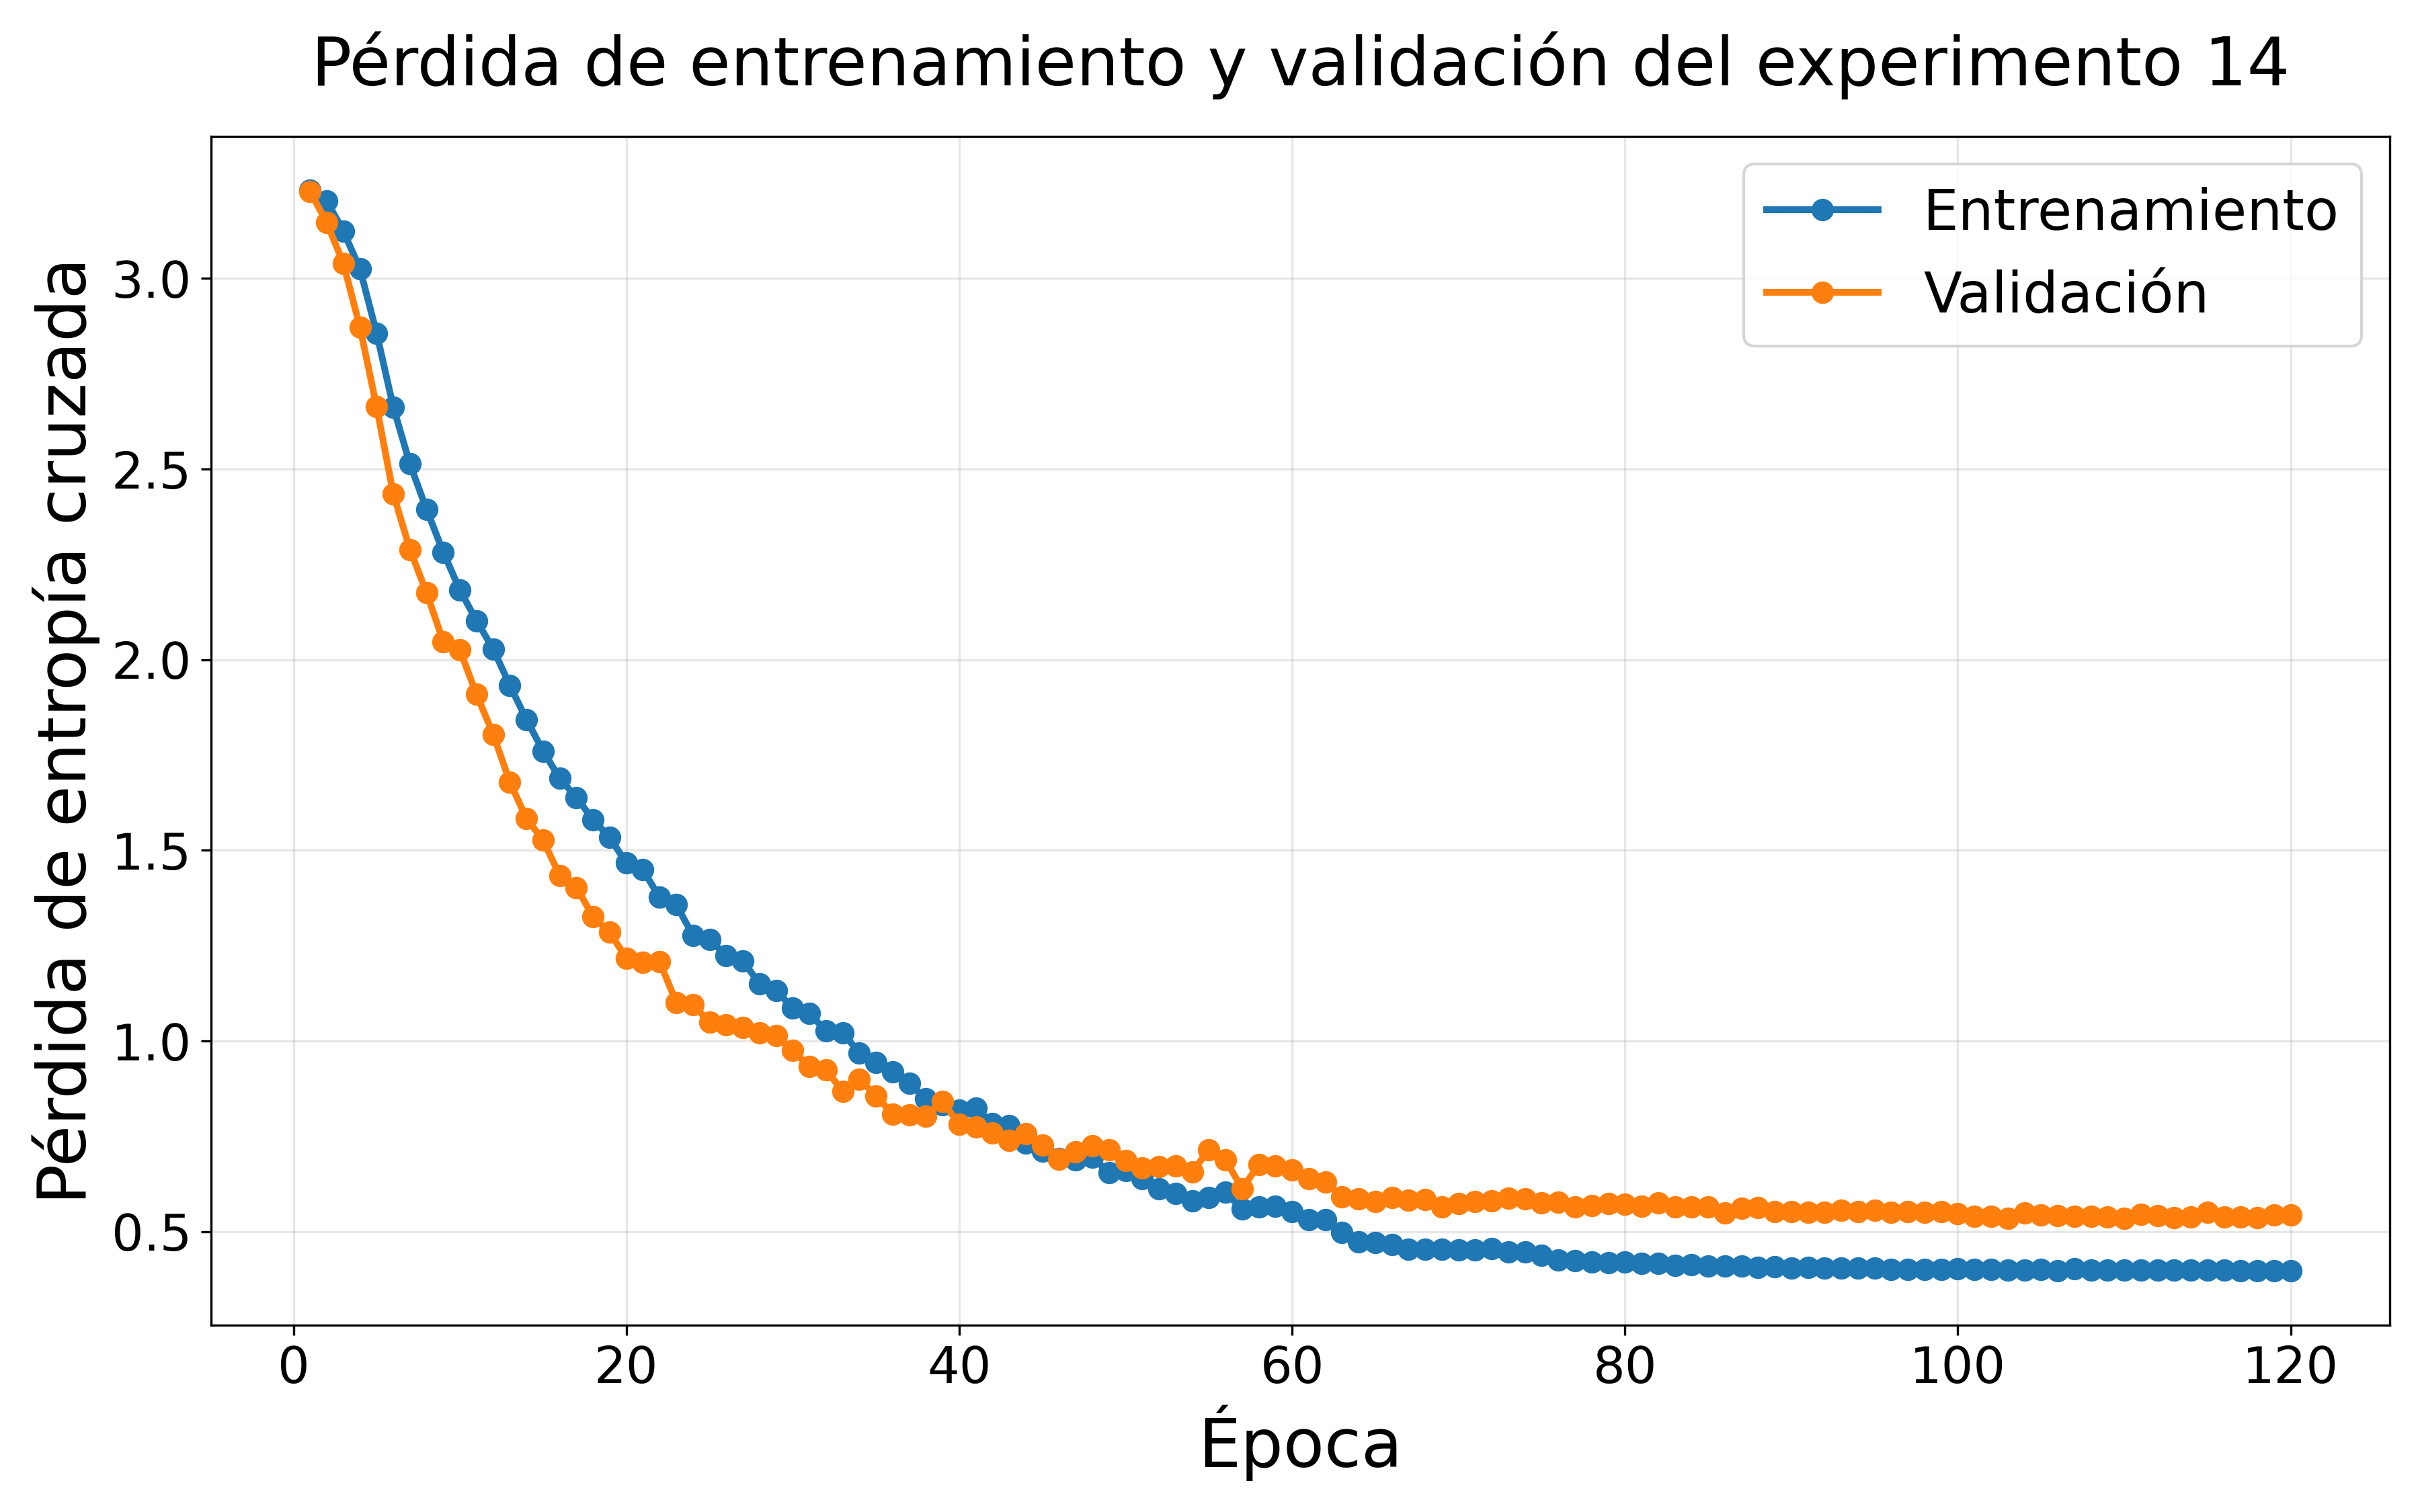
\includegraphics[width=\textwidth]{figures/Experiments_logs/loss_curve_05-11-0958.png}
        \caption{}
        \label{fig:loss_curve_05-11-0958}
    \end{subfigure}

     \vspace{0.4cm}

    \begin{subfigure}{0.45\textwidth}
        \centering
        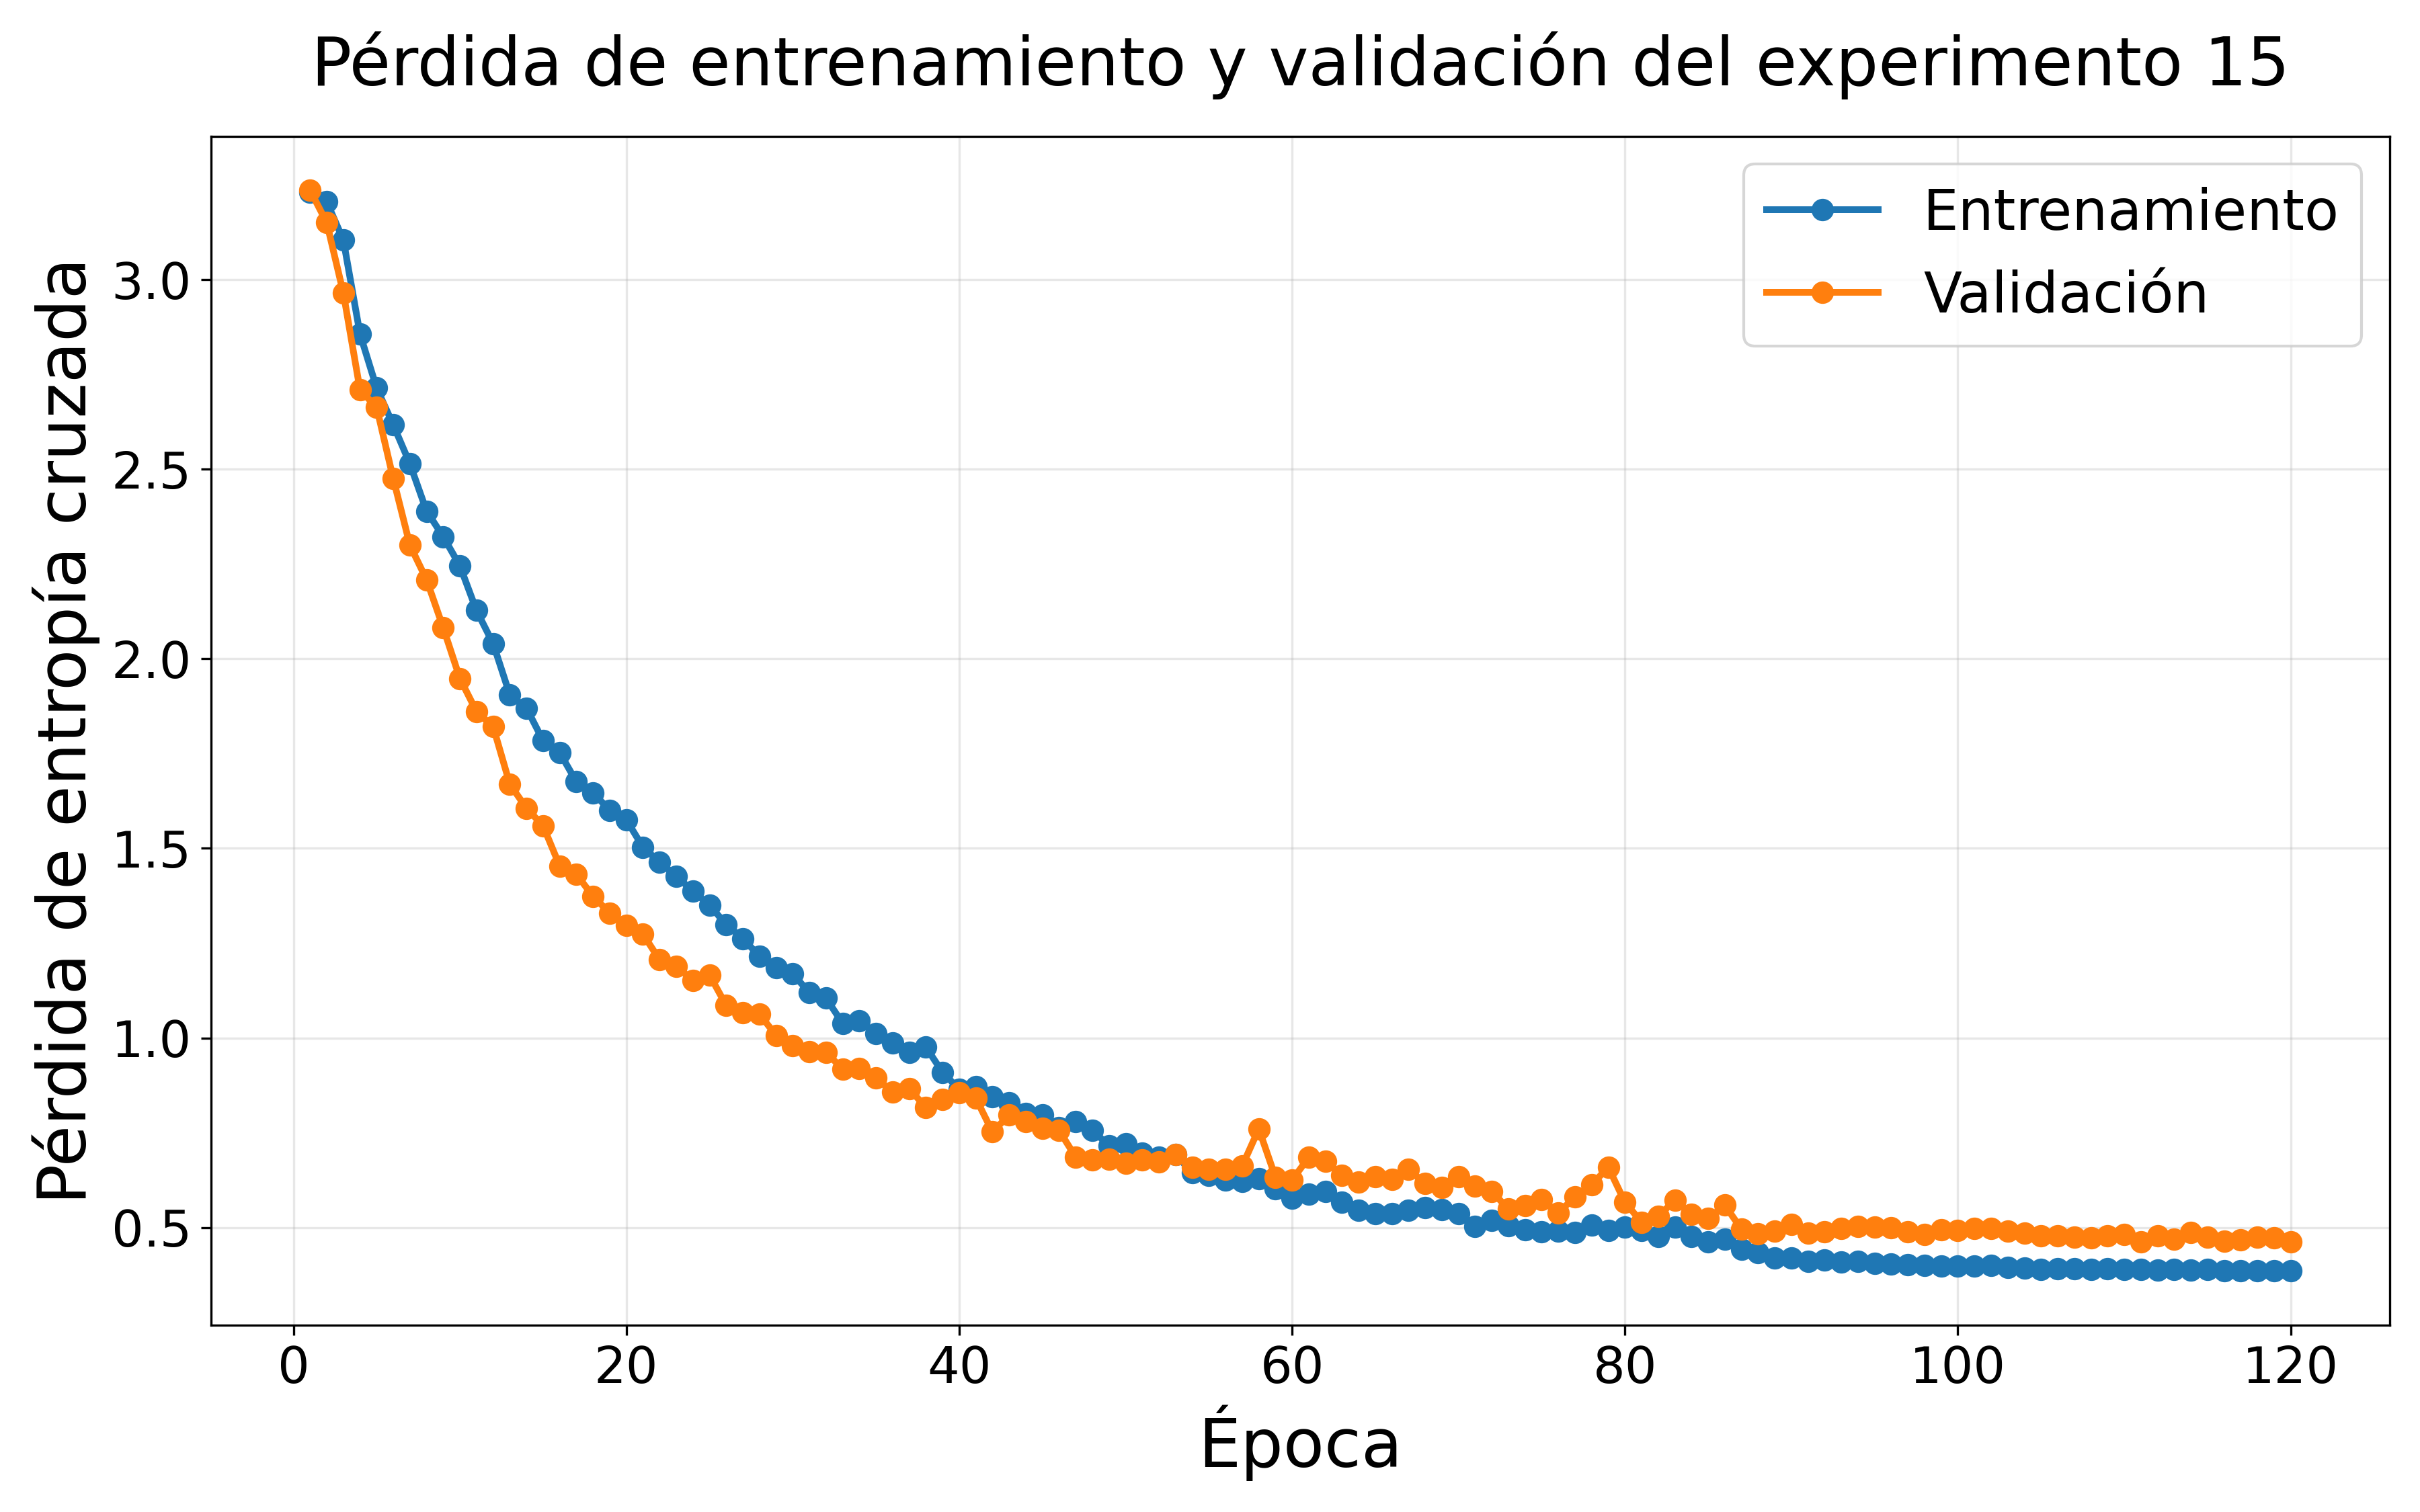
\includegraphics[width=\textwidth]{figures/Experiments_logs/loss_curve_05-11-1101.png}
        \caption{}
        \label{fig:loss_curve_05-11-1101}
    \end{subfigure}

    \caption{Distintos experimentos a los que se le fueron aplicando pequeñas mejoras detalladas en \tabref{tab:ajustes_entrenamiento}. Se puede ver como las curvas de perdida van mejorando con cada experimento.}
    \label{fig:loss_curve-07-11}
\end{figure}

\begin{table}[H]
\centering
\small
\begin{tabularx}{\textwidth}{lXcccc}
\toprule
\textbf{Experimento} & \textbf{Cambio principal} & \textbf{Mejor acc.} & \textbf{Top-5} & \textbf{Mejor loss} & \textbf{Acc. final} \\
\midrule
\texttt{11} & Warmup con configuración 8/8 & 78,46\% & 94,62\% & 1,0915 & 78,03\% \\
\texttt{12} & Subida a dimensión 12/12 & 81,55\% & 95,41\% & 0,8637 & 80,33\% \\
\texttt{13} & Warmup coseno, preservación de aspecto y $L_2$ suave & 86,86\% & 97,77\% & 0,7065 & 86,43\% \\
\texttt{14} & Label smoothing 0,05, seed 42 & 87,08\% & 96,77\% & 0,5221 & 86,93\% \\
\texttt{15} & Repetición del experimento con label smoothing 0,05 & 88,94\% & 97,20\% & 0,4617 & 88,44\% \\
\bottomrule
\end{tabularx}
\caption{Evolución de los ajustes de entrenamiento antes del último cambio de \textit{data augmentation}.}
\label{tab:ajustes_entrenamiento}
\end{table}

El \textit{warmup} ayudó a que el entrenamiento no empezara de forma tan agresiva. Subir \texttt{local\_dim} y \texttt{bond\_dim} a 12 también mejoró bastante, porque la representación que entraba en la TTN y el vector interno de enlace tenían más capacidad.

Después, la combinación de warmup coseno mas la preservación de relación de aspecto de las imágenes recortadas y la implementación de un término de regularización $L_2$, llevó el modelo hasta 86,86\% de precisión. En este punto el modelo ya funcionaba bien, pero seguía habiendo sobreconfianza en los errores. Por eso se incorporó \textit{label smoothing}. Con \texttt{label\_smoothing=0.05} no solo mejoró ligeramente la precisión, sino que bajó de forma clara la pérdida de evaluación y la confianza media cuando el modelo se equivocaba.

\begin{figure}[htbp]
    \centering
    \captionsetup[subfigure]{skip=1pt}
    \captionsetup[figure]{font=footnotesize, skip=3pt}
    
    \begin{subfigure}{0.45\textwidth}
        \centering
        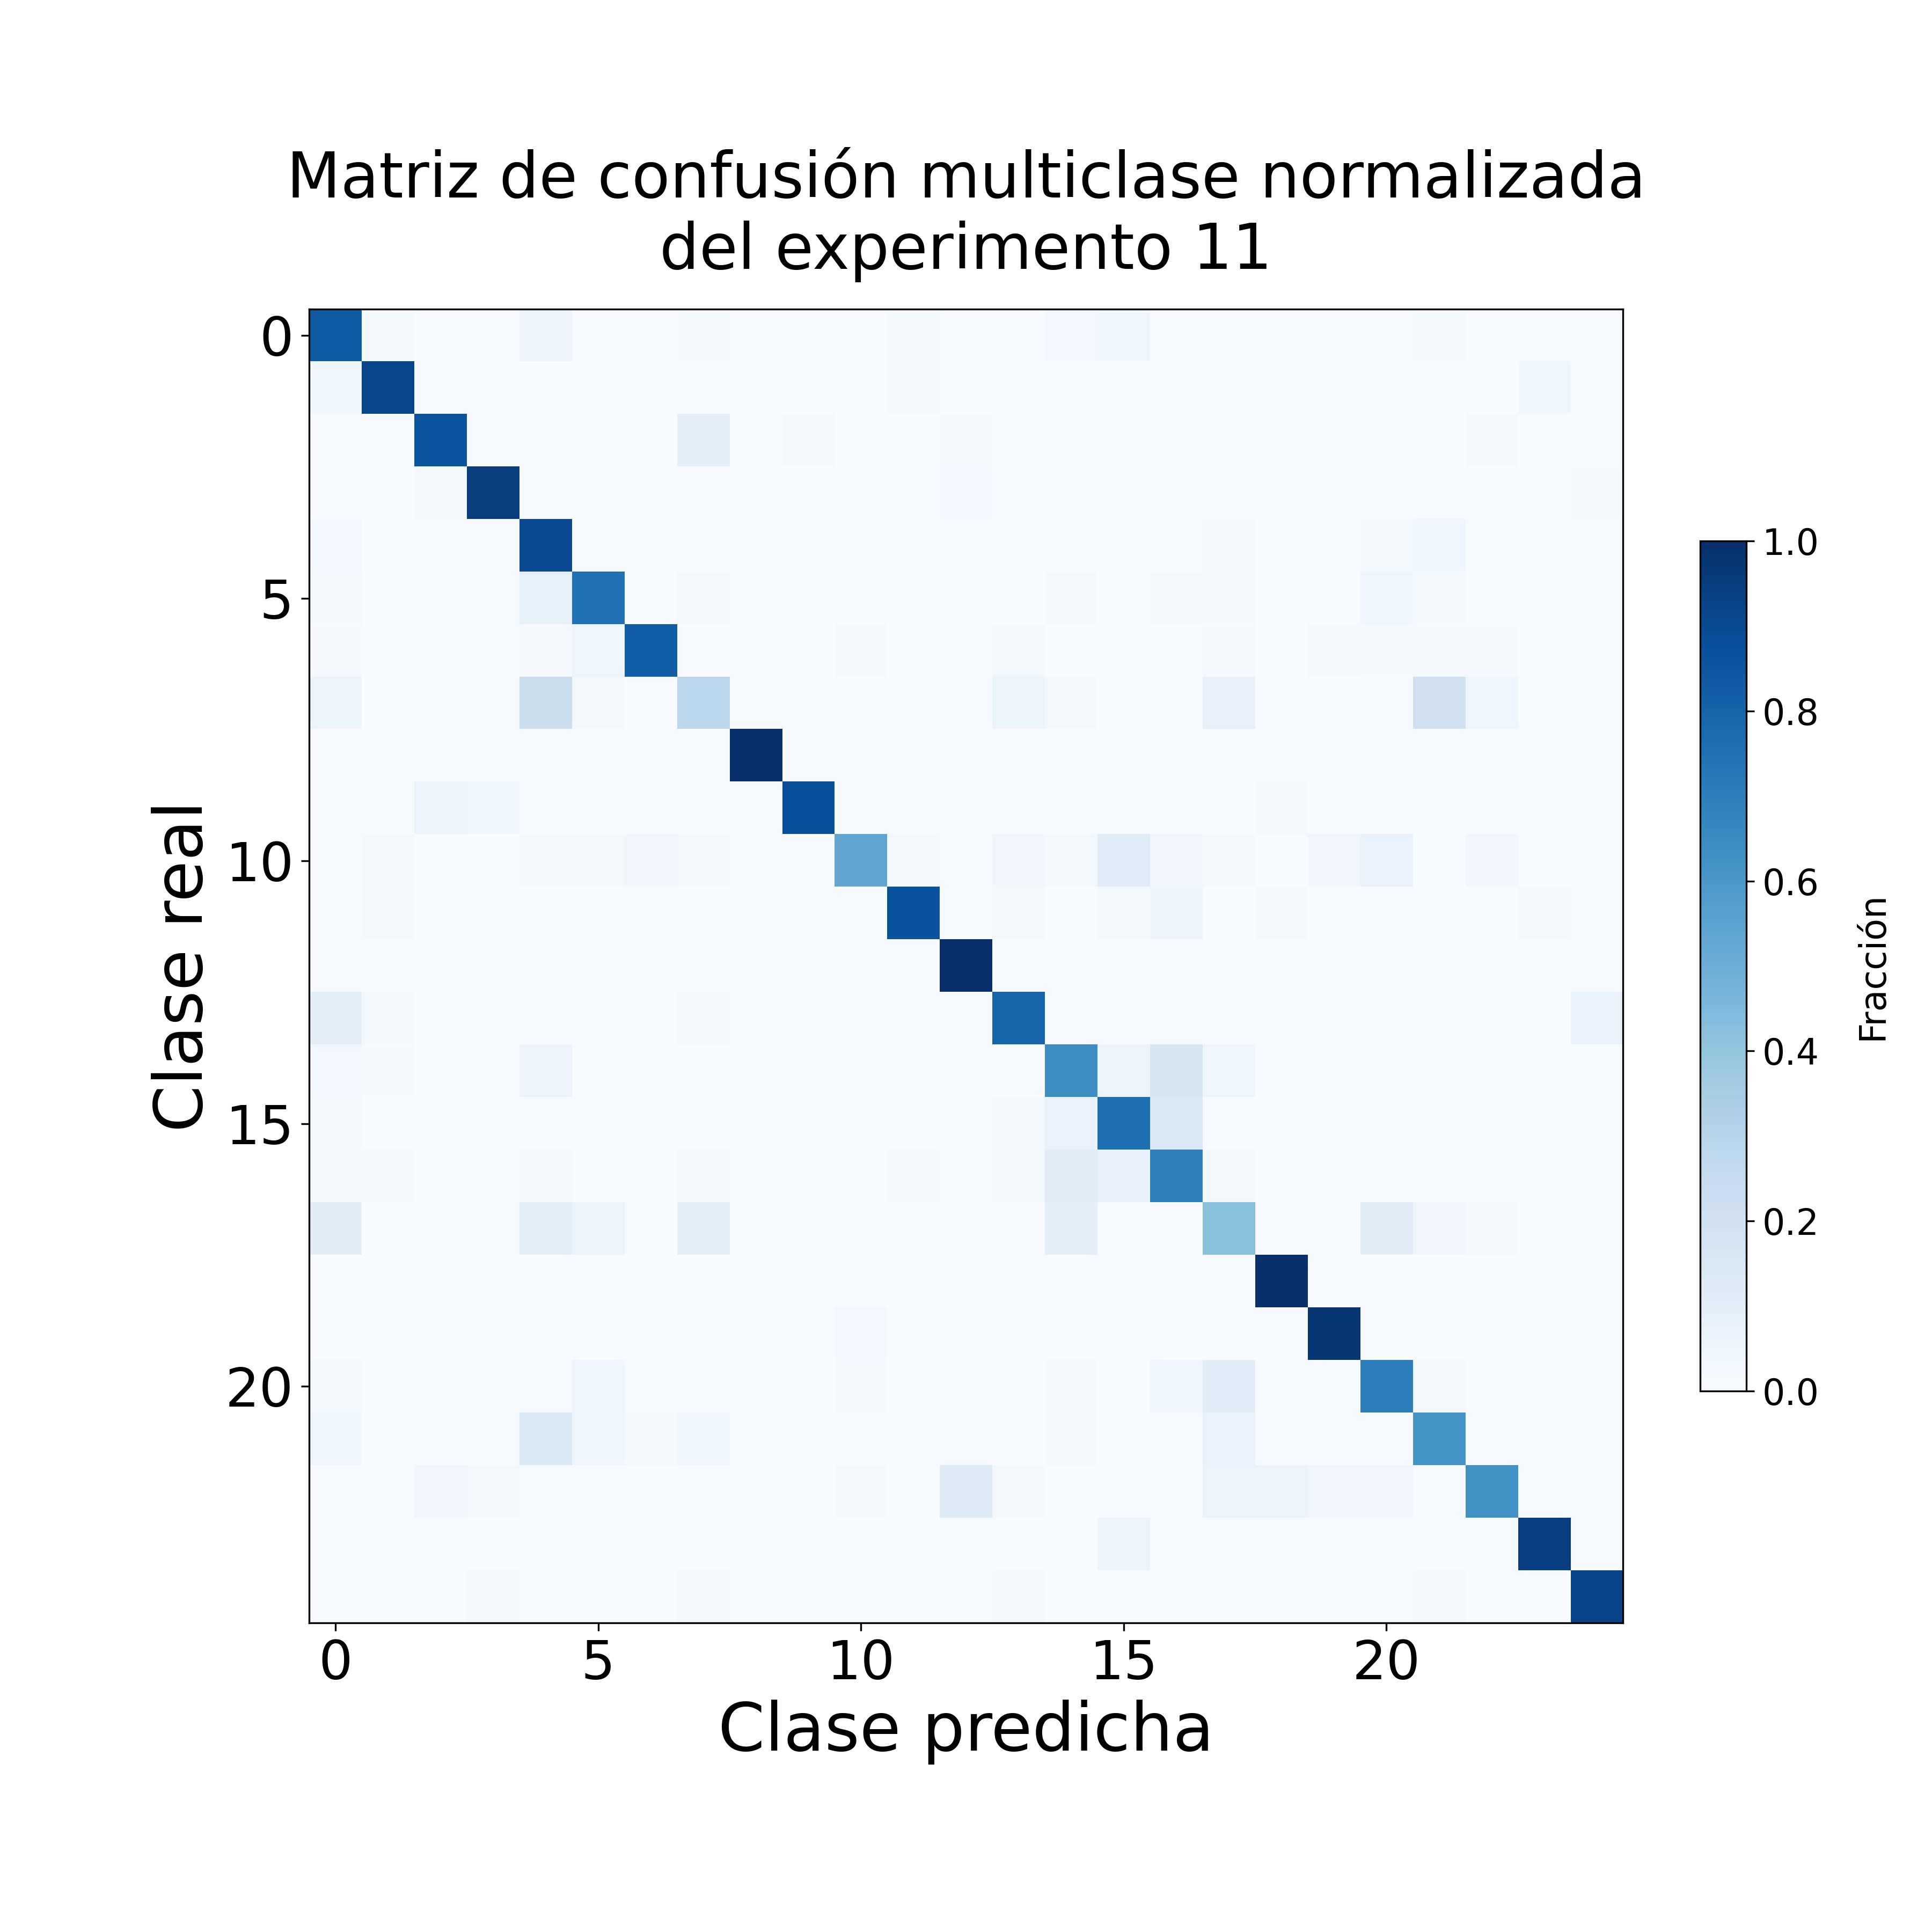
\includegraphics[width=\textwidth]{figures/Experiments_logs/confusion_matrix_05-07-0857.png}
        \caption{}
        \label{fig:confusion_matrix_05-07-0857}
    \end{subfigure}
    \hfill
    \begin{subfigure}{0.45\textwidth}
        \centering
        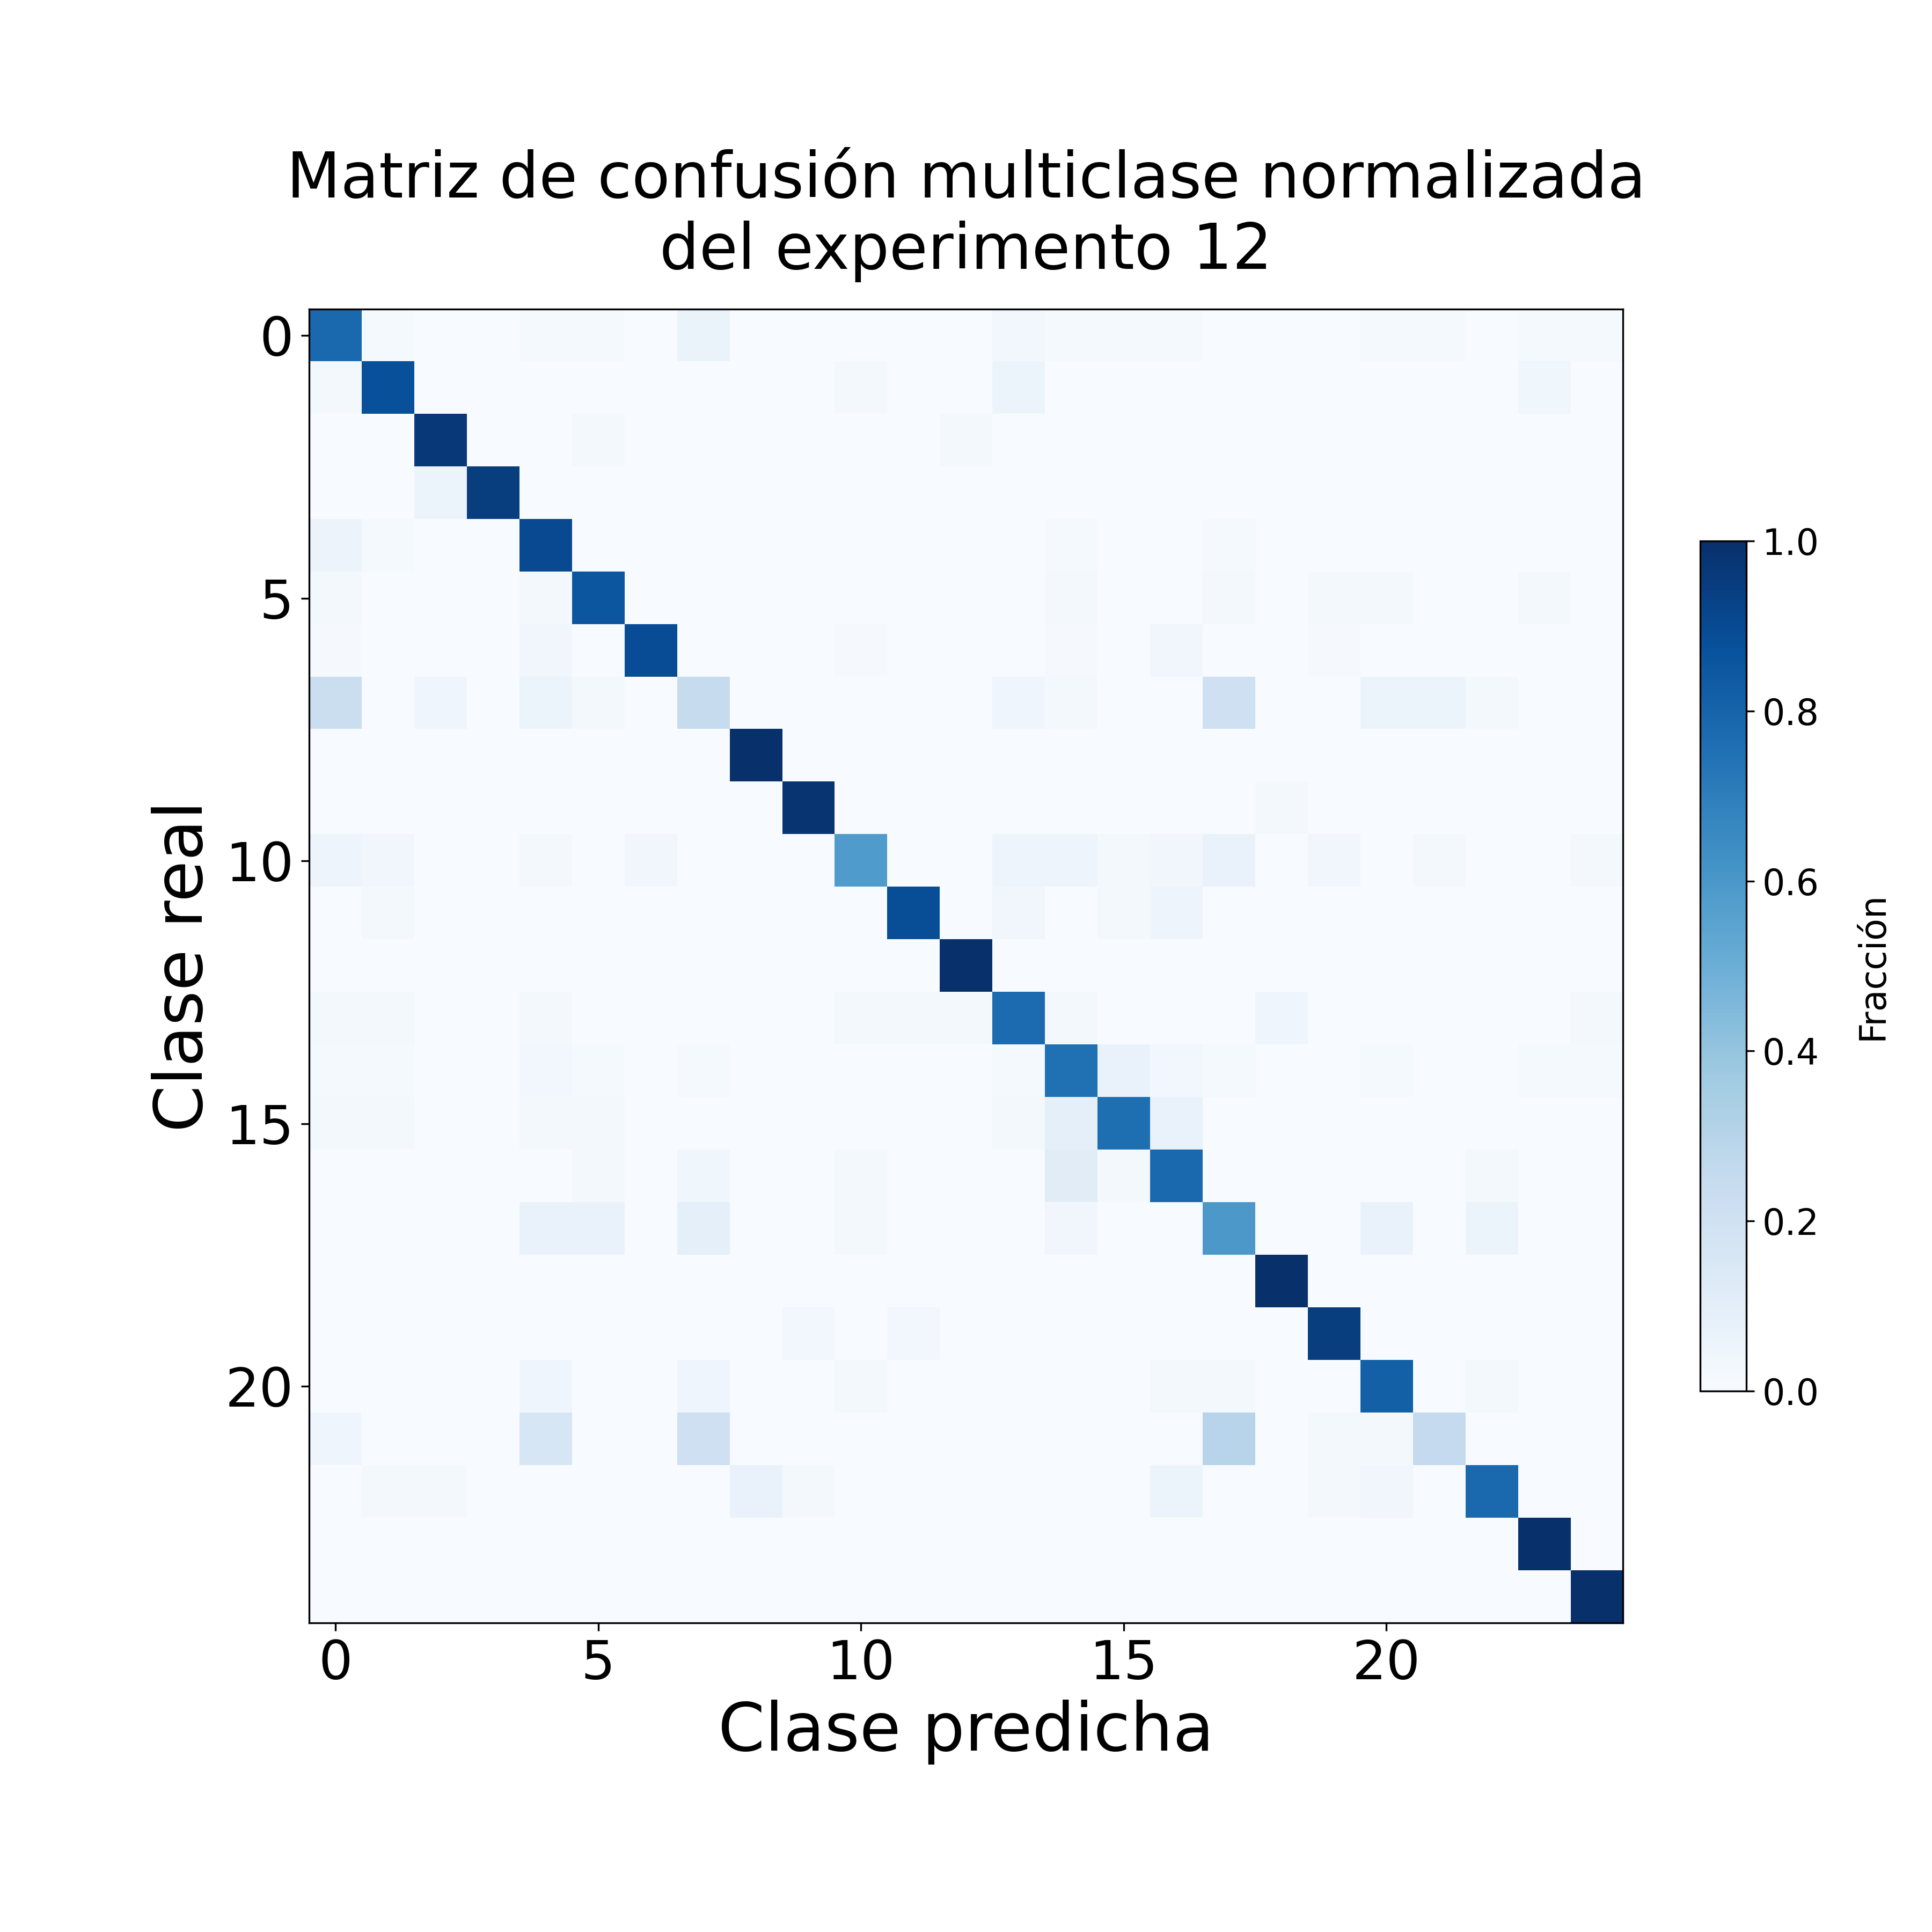
\includegraphics[width=\textwidth]{figures/Experiments_logs/confusion_matrix_05-07-1304.png}
        \caption{}
        \label{fig:confusion_matrix_05-07-1304}
    \end{subfigure}

    \vspace{0.08cm}

    \begin{subfigure}{0.45\textwidth}
        \centering
        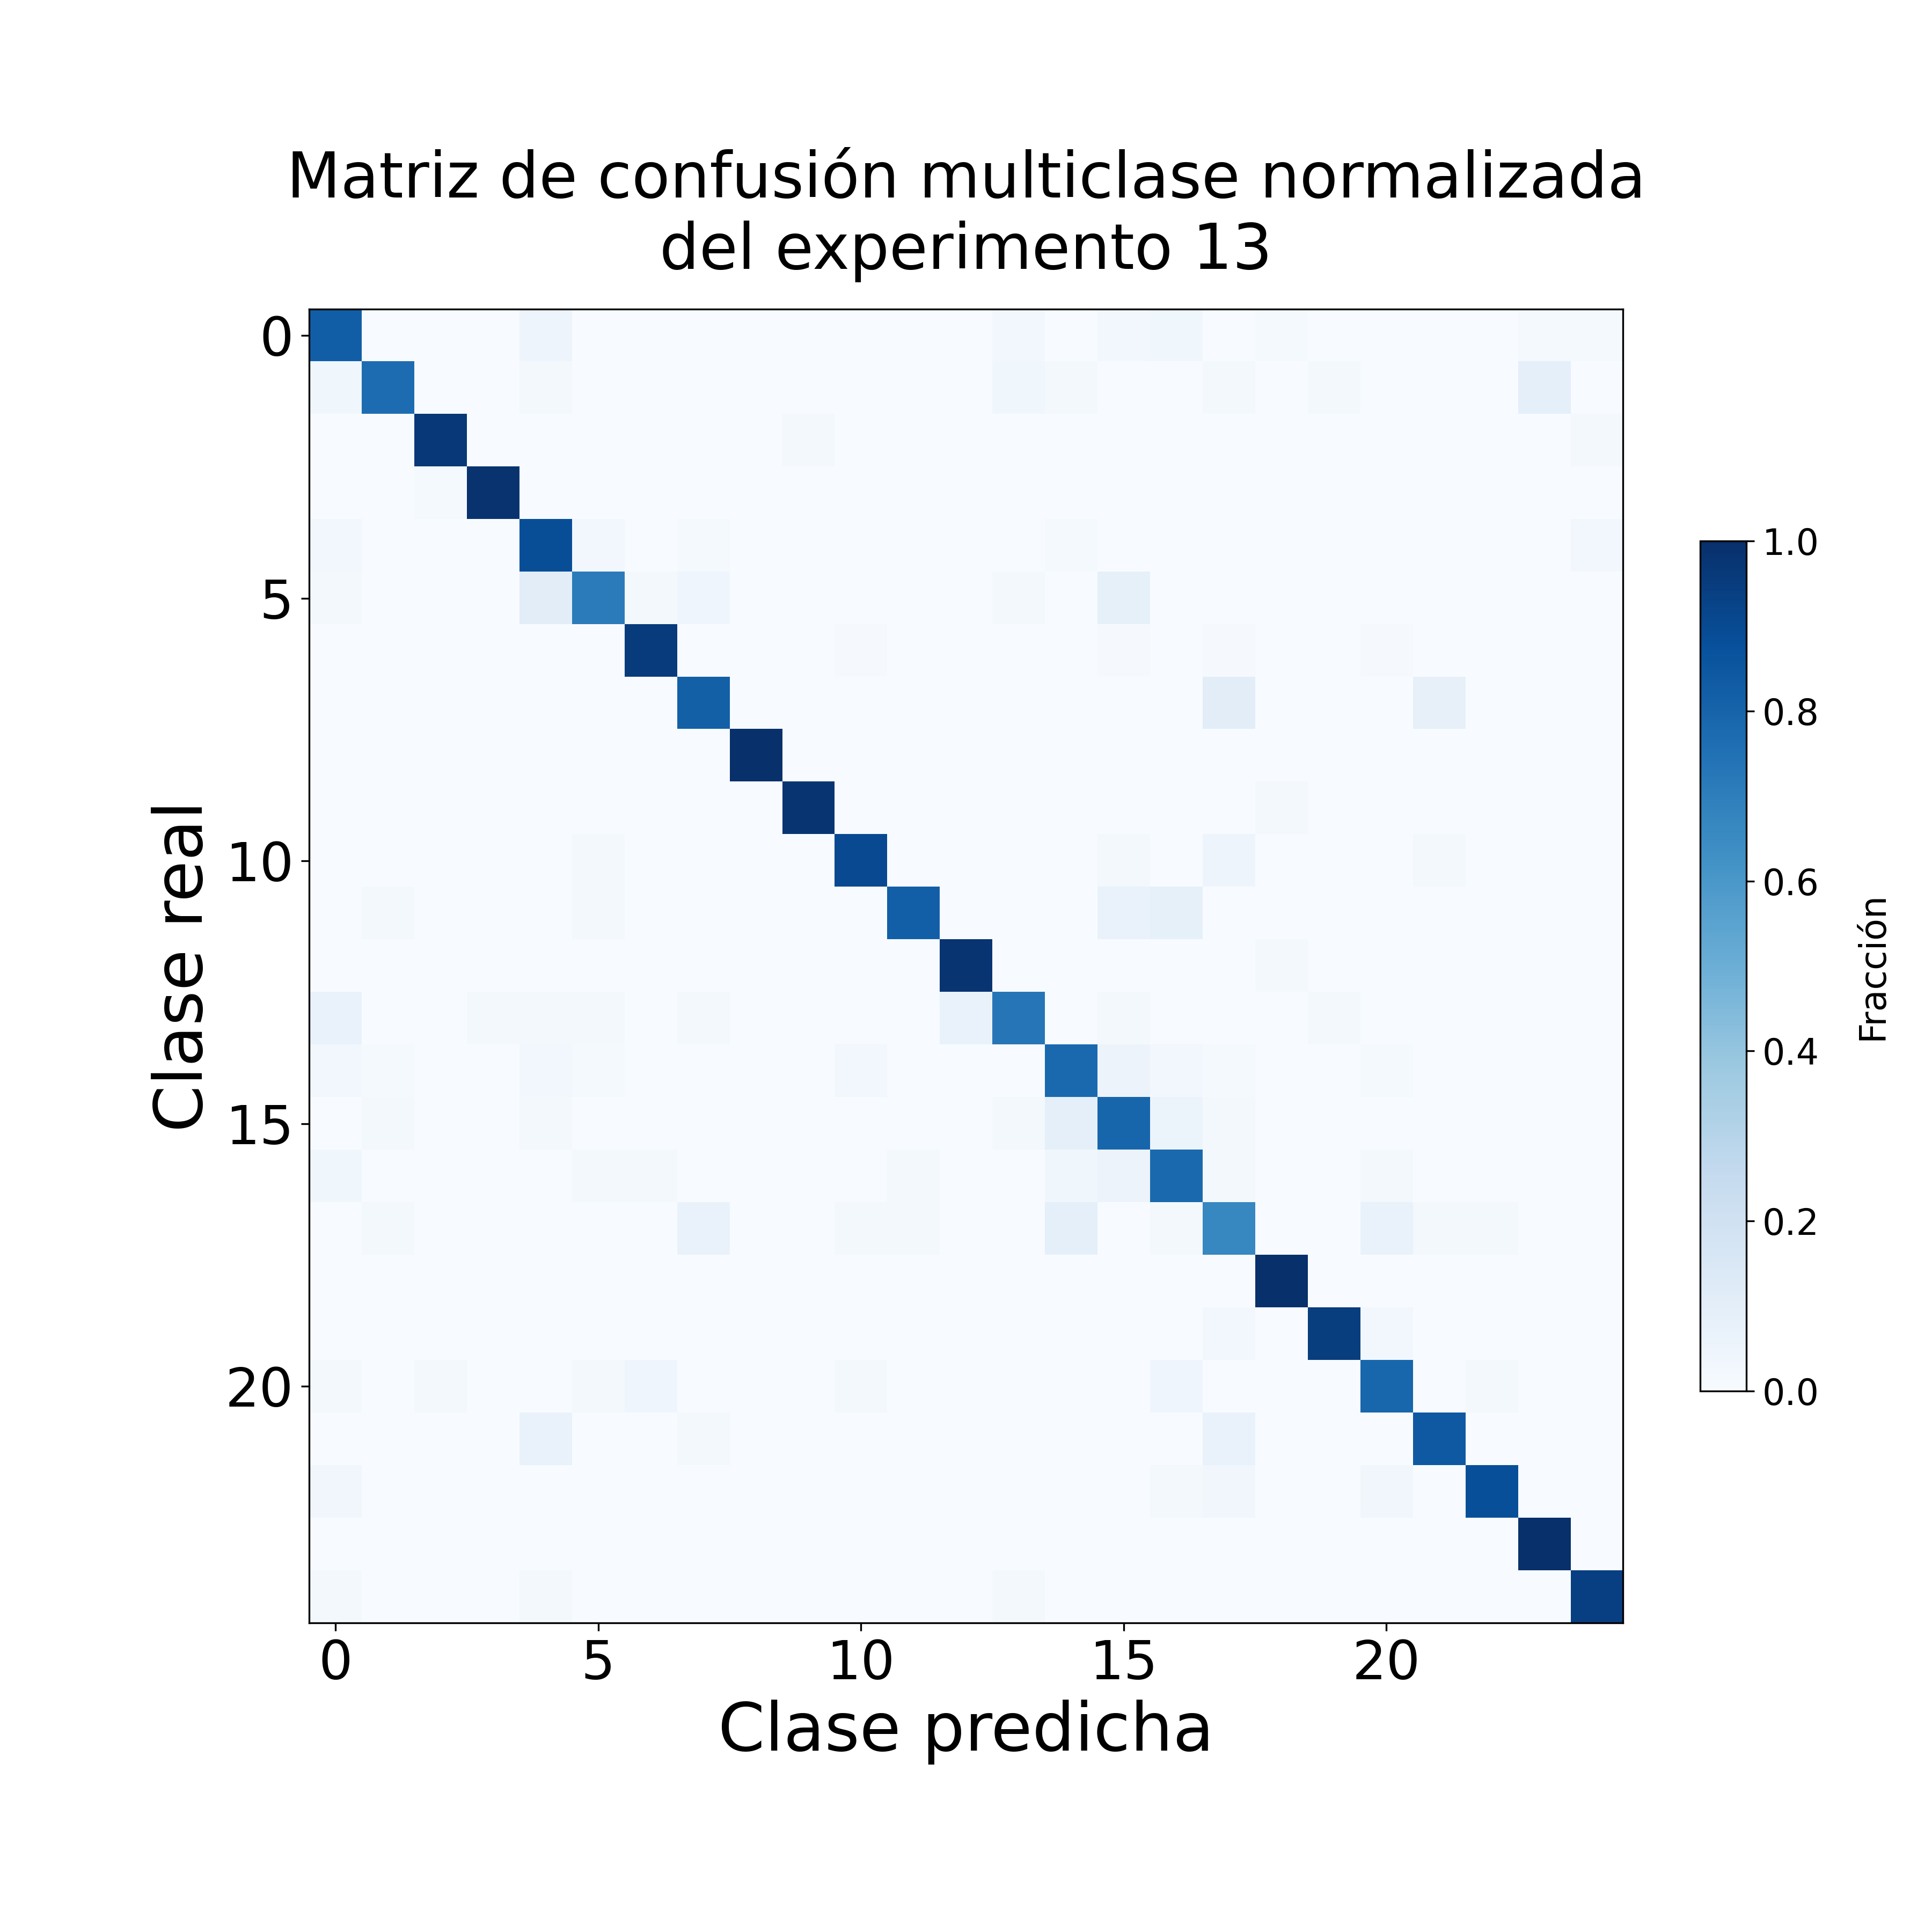
\includegraphics[width=\textwidth]{figures/Experiments_logs/confusion_matrix_05-08-1400.png}
        \caption{}
        \label{fig:confusion_matrix_05-08-1400}
    \end{subfigure}
    \hfill
    \begin{subfigure}{0.45\textwidth}
        \centering
        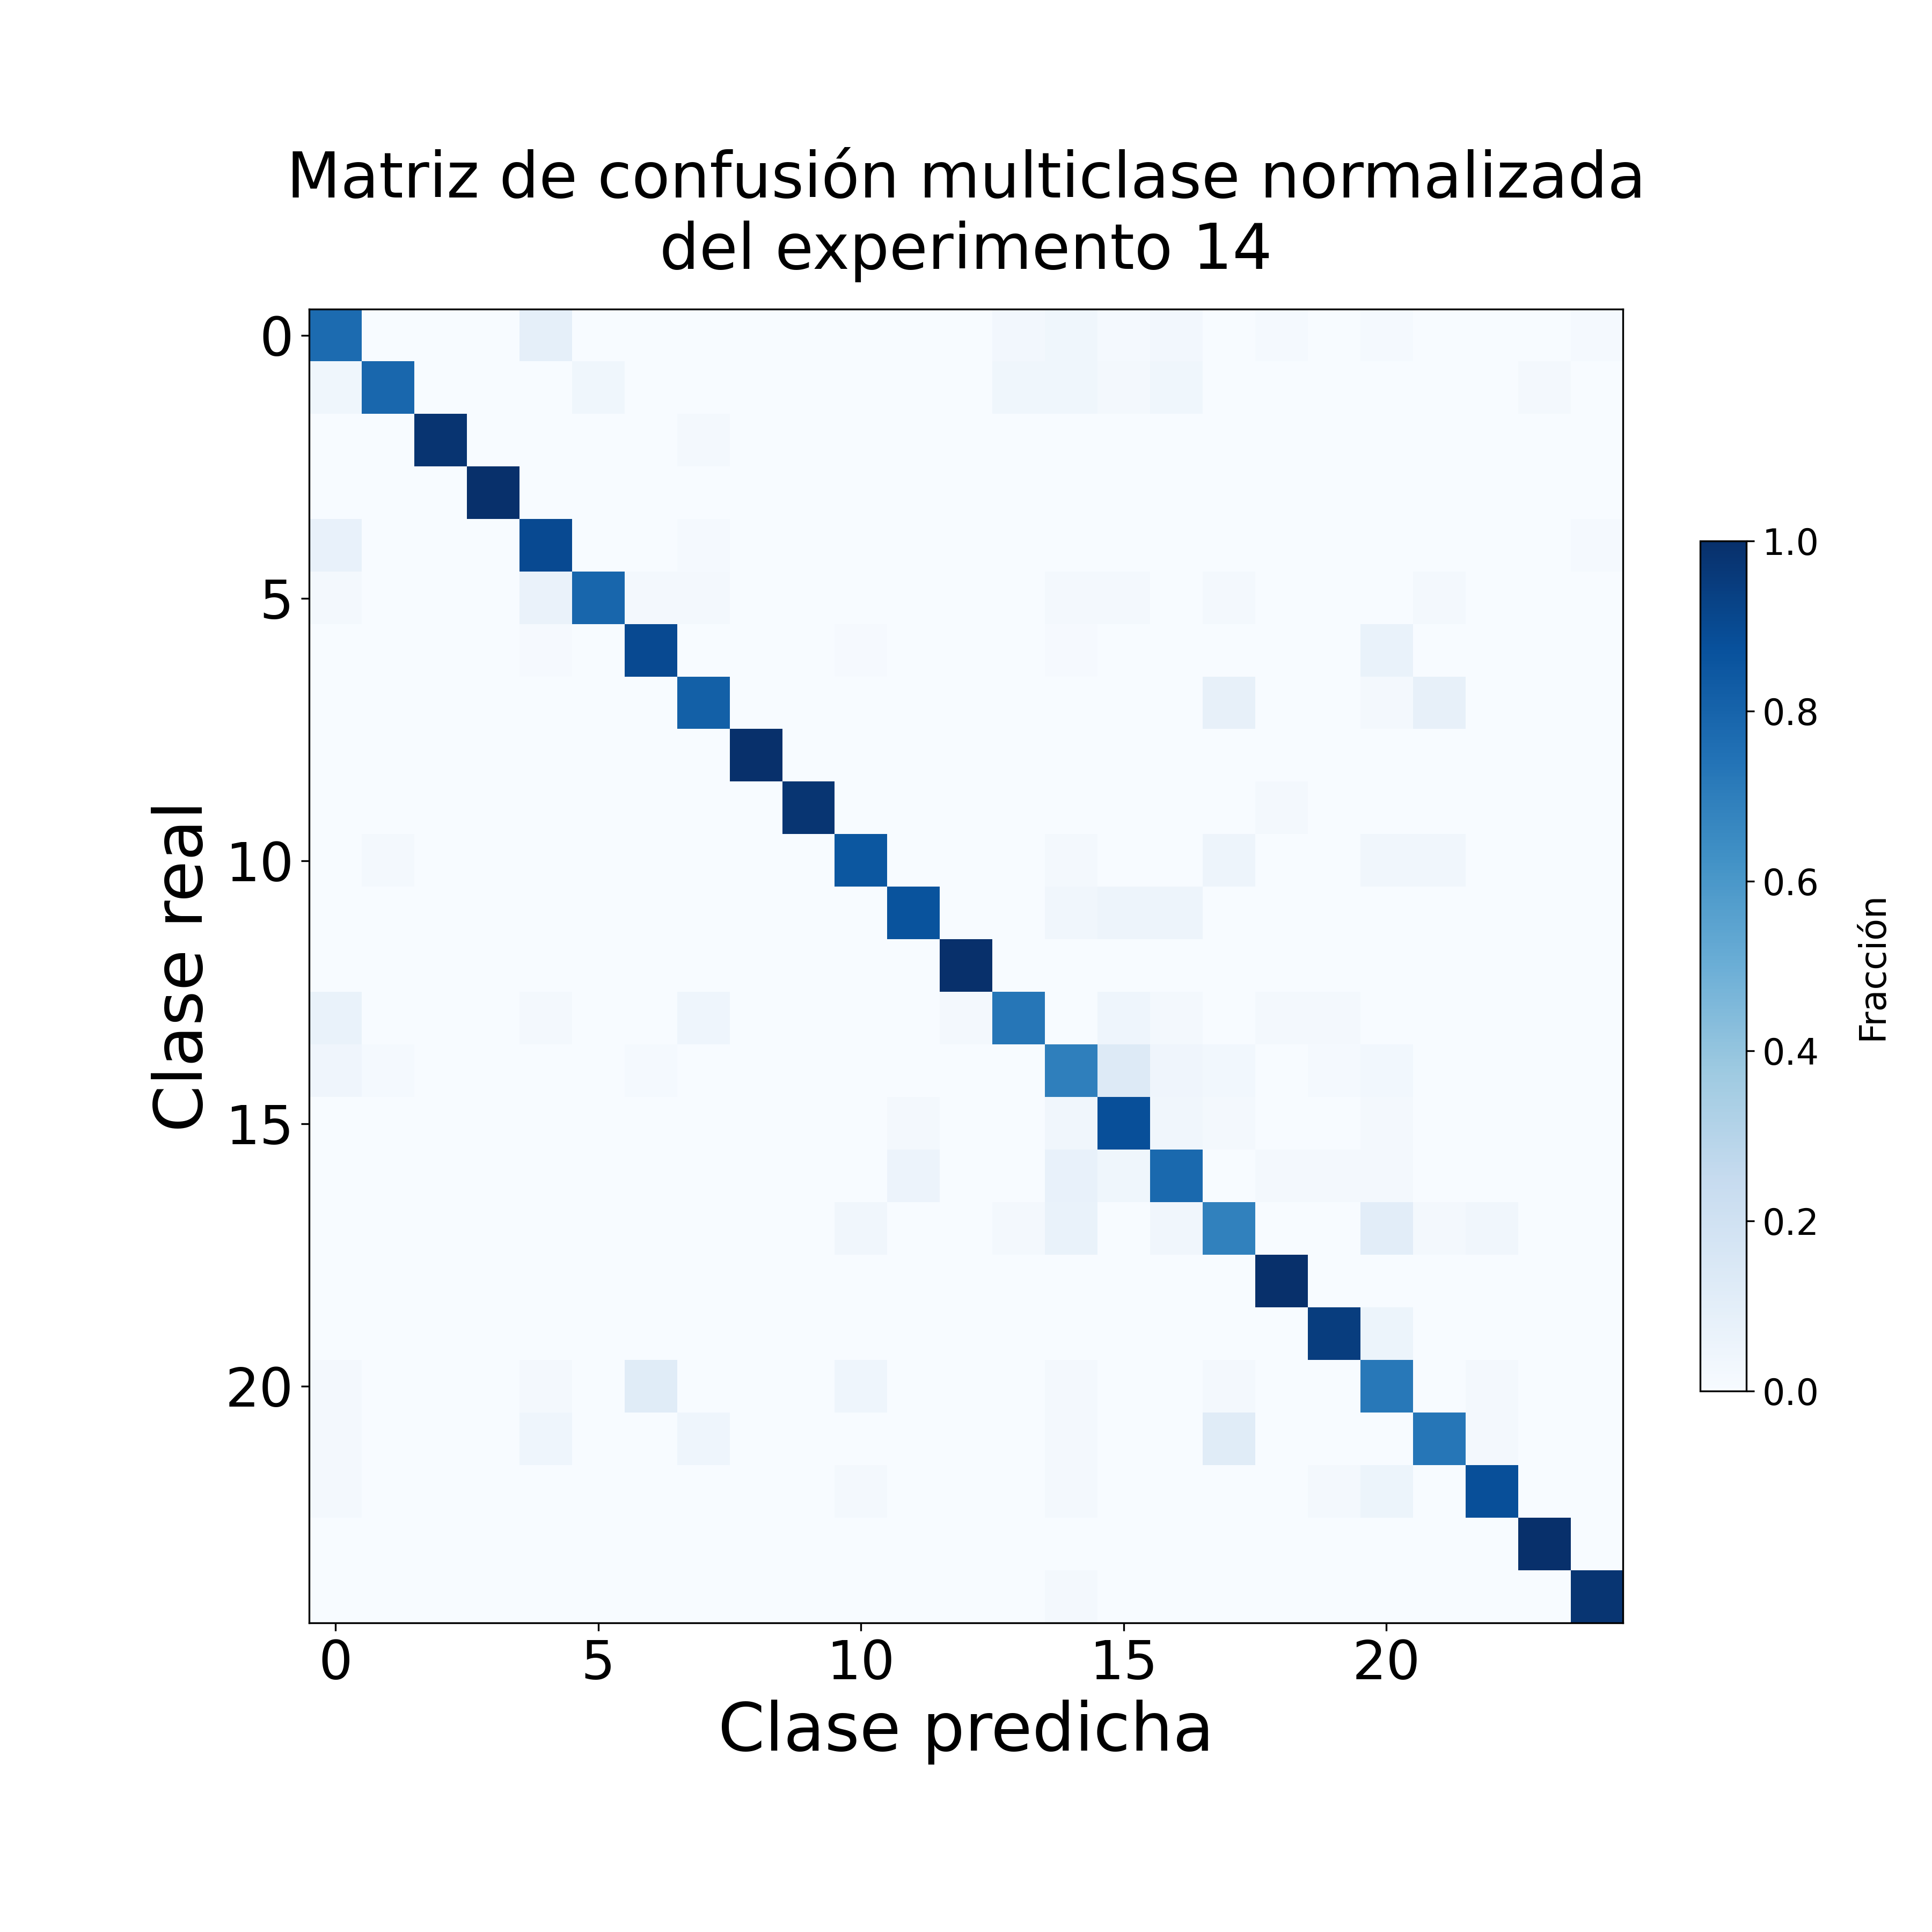
\includegraphics[width=\textwidth]{figures/Experiments_logs/confusion_matrix_05-11-0958.png}
        \caption{}
        \label{fig:confusion_matrix_05-11-0958}
    \end{subfigure}

     \vspace{0.08cm}

    \begin{subfigure}{0.45\textwidth}
        \centering
        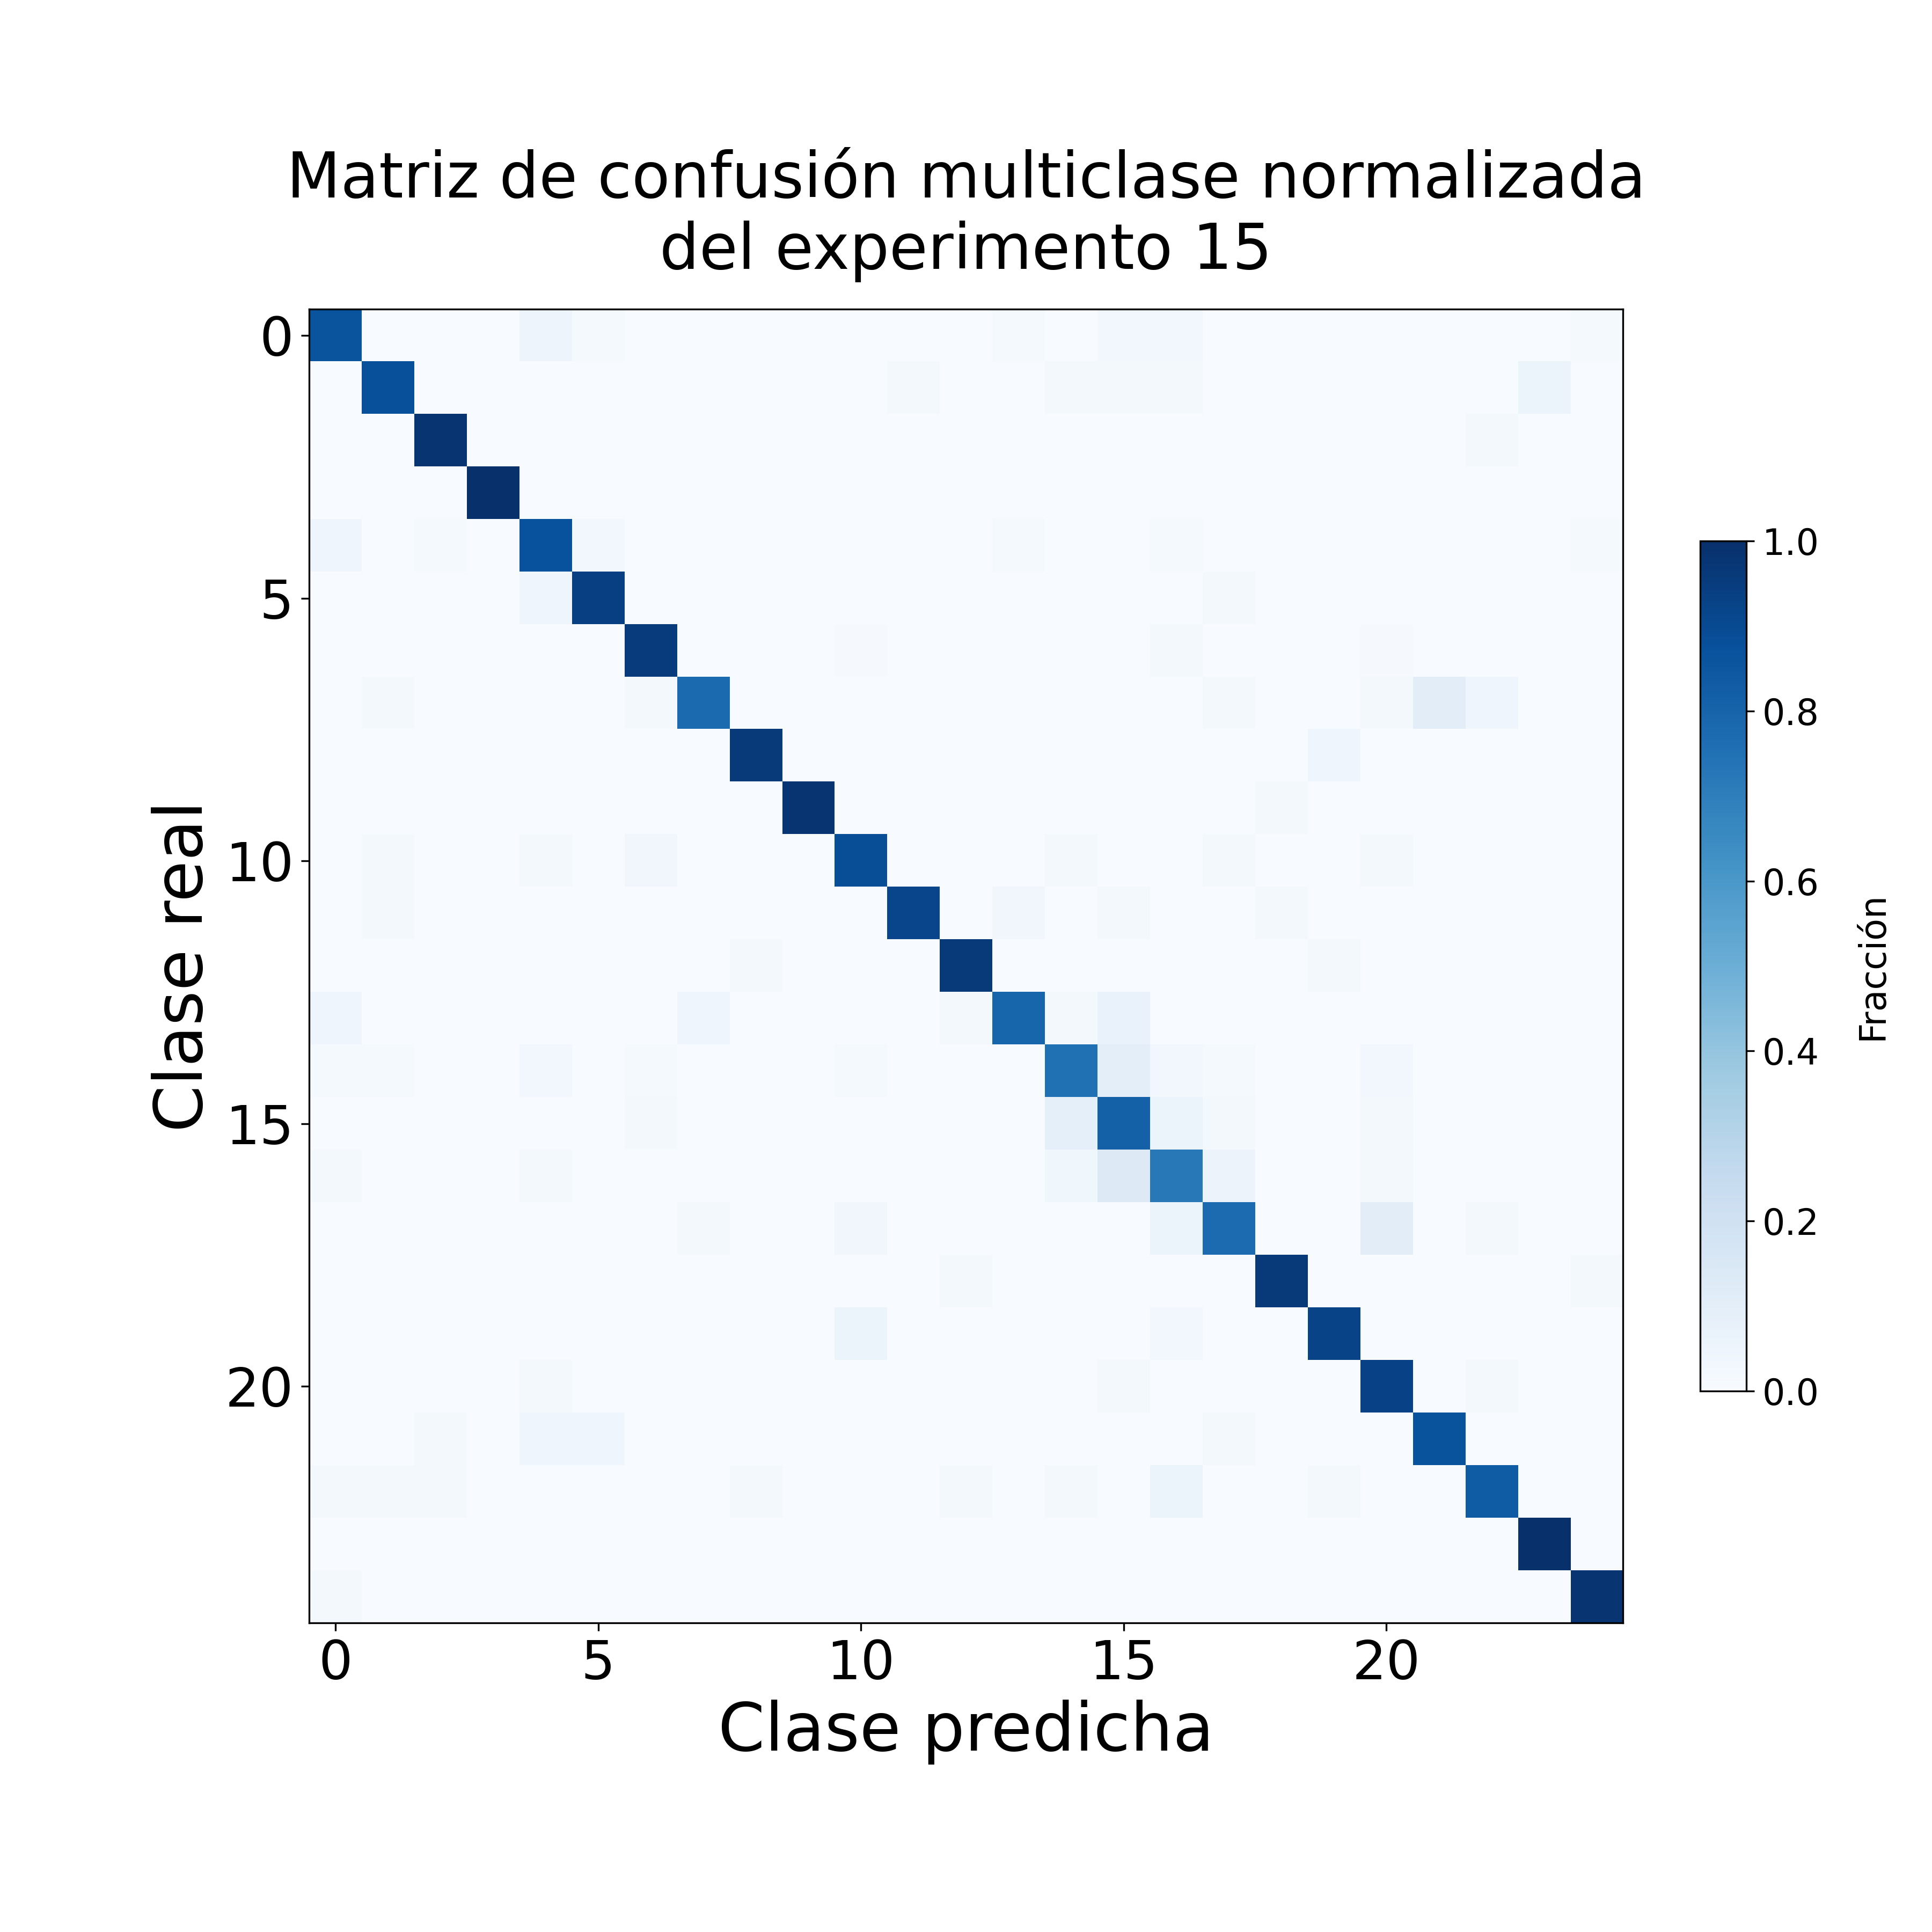
\includegraphics[width=\textwidth]{figures/Experiments_logs/confusion_matrix_05-11-1101.png}
        \caption{}
        \label{fig:confusion_matrix_05-11-1101}
    \end{subfigure}
    
    \caption{Matrices de confusión de distintos experimentos a los que se le fueron aplicando pequeñas mejoras detalladas en \tabref{tab:ajustes_entrenamiento}. Se puede ver como la diagonal se hace más evidente a medida que se aplican los cambios.}
    \label{fig:confusion_matrix-07-11}
\end{figure}

Las clases difíciles seguían siendo bastante coherentes entre experimentos, objetos alargados o muy parecidos entre sí, como \textit{Measuring Cylinder}, \textit{Volumetric Flask}, \textit{Separating Funnel}, \textit{Test Tube}, \textit{Pipette} y las distintas variantes de \textit{Round Bottom Flask}. Esto era una señal importante, los errores no eran aleatorios, sino que estaban concentrados en formas visualmente parecidas.

\subsection{Hipótesis 4}

La cuarta hipótesis fue que el modelo no necesitaba solo más capacidad, sino ver variaciones suaves de esos objetos durante el entrenamiento. Si el modelo confundía clases parecidas por pequeñas diferencias de forma, orientación o visibilidad, entonces una \textit{data augmentation} más adecuada podía ayudar a aprender representaciones más robustas.

Por eso se introdujo una opción de aumento \texttt{light}, con rotaciones pequeñas y borrado aleatorio bajo. No se buscaba deformar agresivamente los objetos, porque en este dataset la geometría importa mucho. La idea era justamente la contraria, simular variaciones más ligeras sin destruir la clase.

\section{Salto con data augmentation light}

El cambio más importante de toda la fase final fue la nueva \textit{data augmentation} suave. Manteniendo la configuración fuerte anterior, se lanzaron cuatro experimentos con seeds distintas:

\begin{table}[H]
\centering
\small
\begin{tabular}{lccccc}
\toprule
\textbf{Experimento} & \textbf{Seed} & \textbf{Mejor acc.} & \textbf{Top-5} & \textbf{Mejor loss} & \textbf{Macro F1} \\
\midrule
\texttt{16} & 55 & 94,54\% & 98,85\% & 0,2684 & 94,64\% \\
\texttt{17} & 42 & 94,19\% & 99,21\% & 0,2503 & 94,26\% \\
\texttt{18} & 69 & 96,05\% & 99,43\% & 0,1997 & 95,94\% \\
\texttt{19} & 111 & 94,26\% & 98,71\% & 0,2634 & 94,28\% \\
\midrule
\textbf{Media} & -- & \textbf{94,76\%} & -- & -- & \textbf{94,78\%} \\
\bottomrule
\end{tabular}
\caption{Resultados con \texttt{augmentation\_name = light}.}
\label{tab:light_augmentation}
\end{table}

\begin{figure}[H]
    \centering

    \begin{subfigure}{0.45\textwidth}
        \centering
        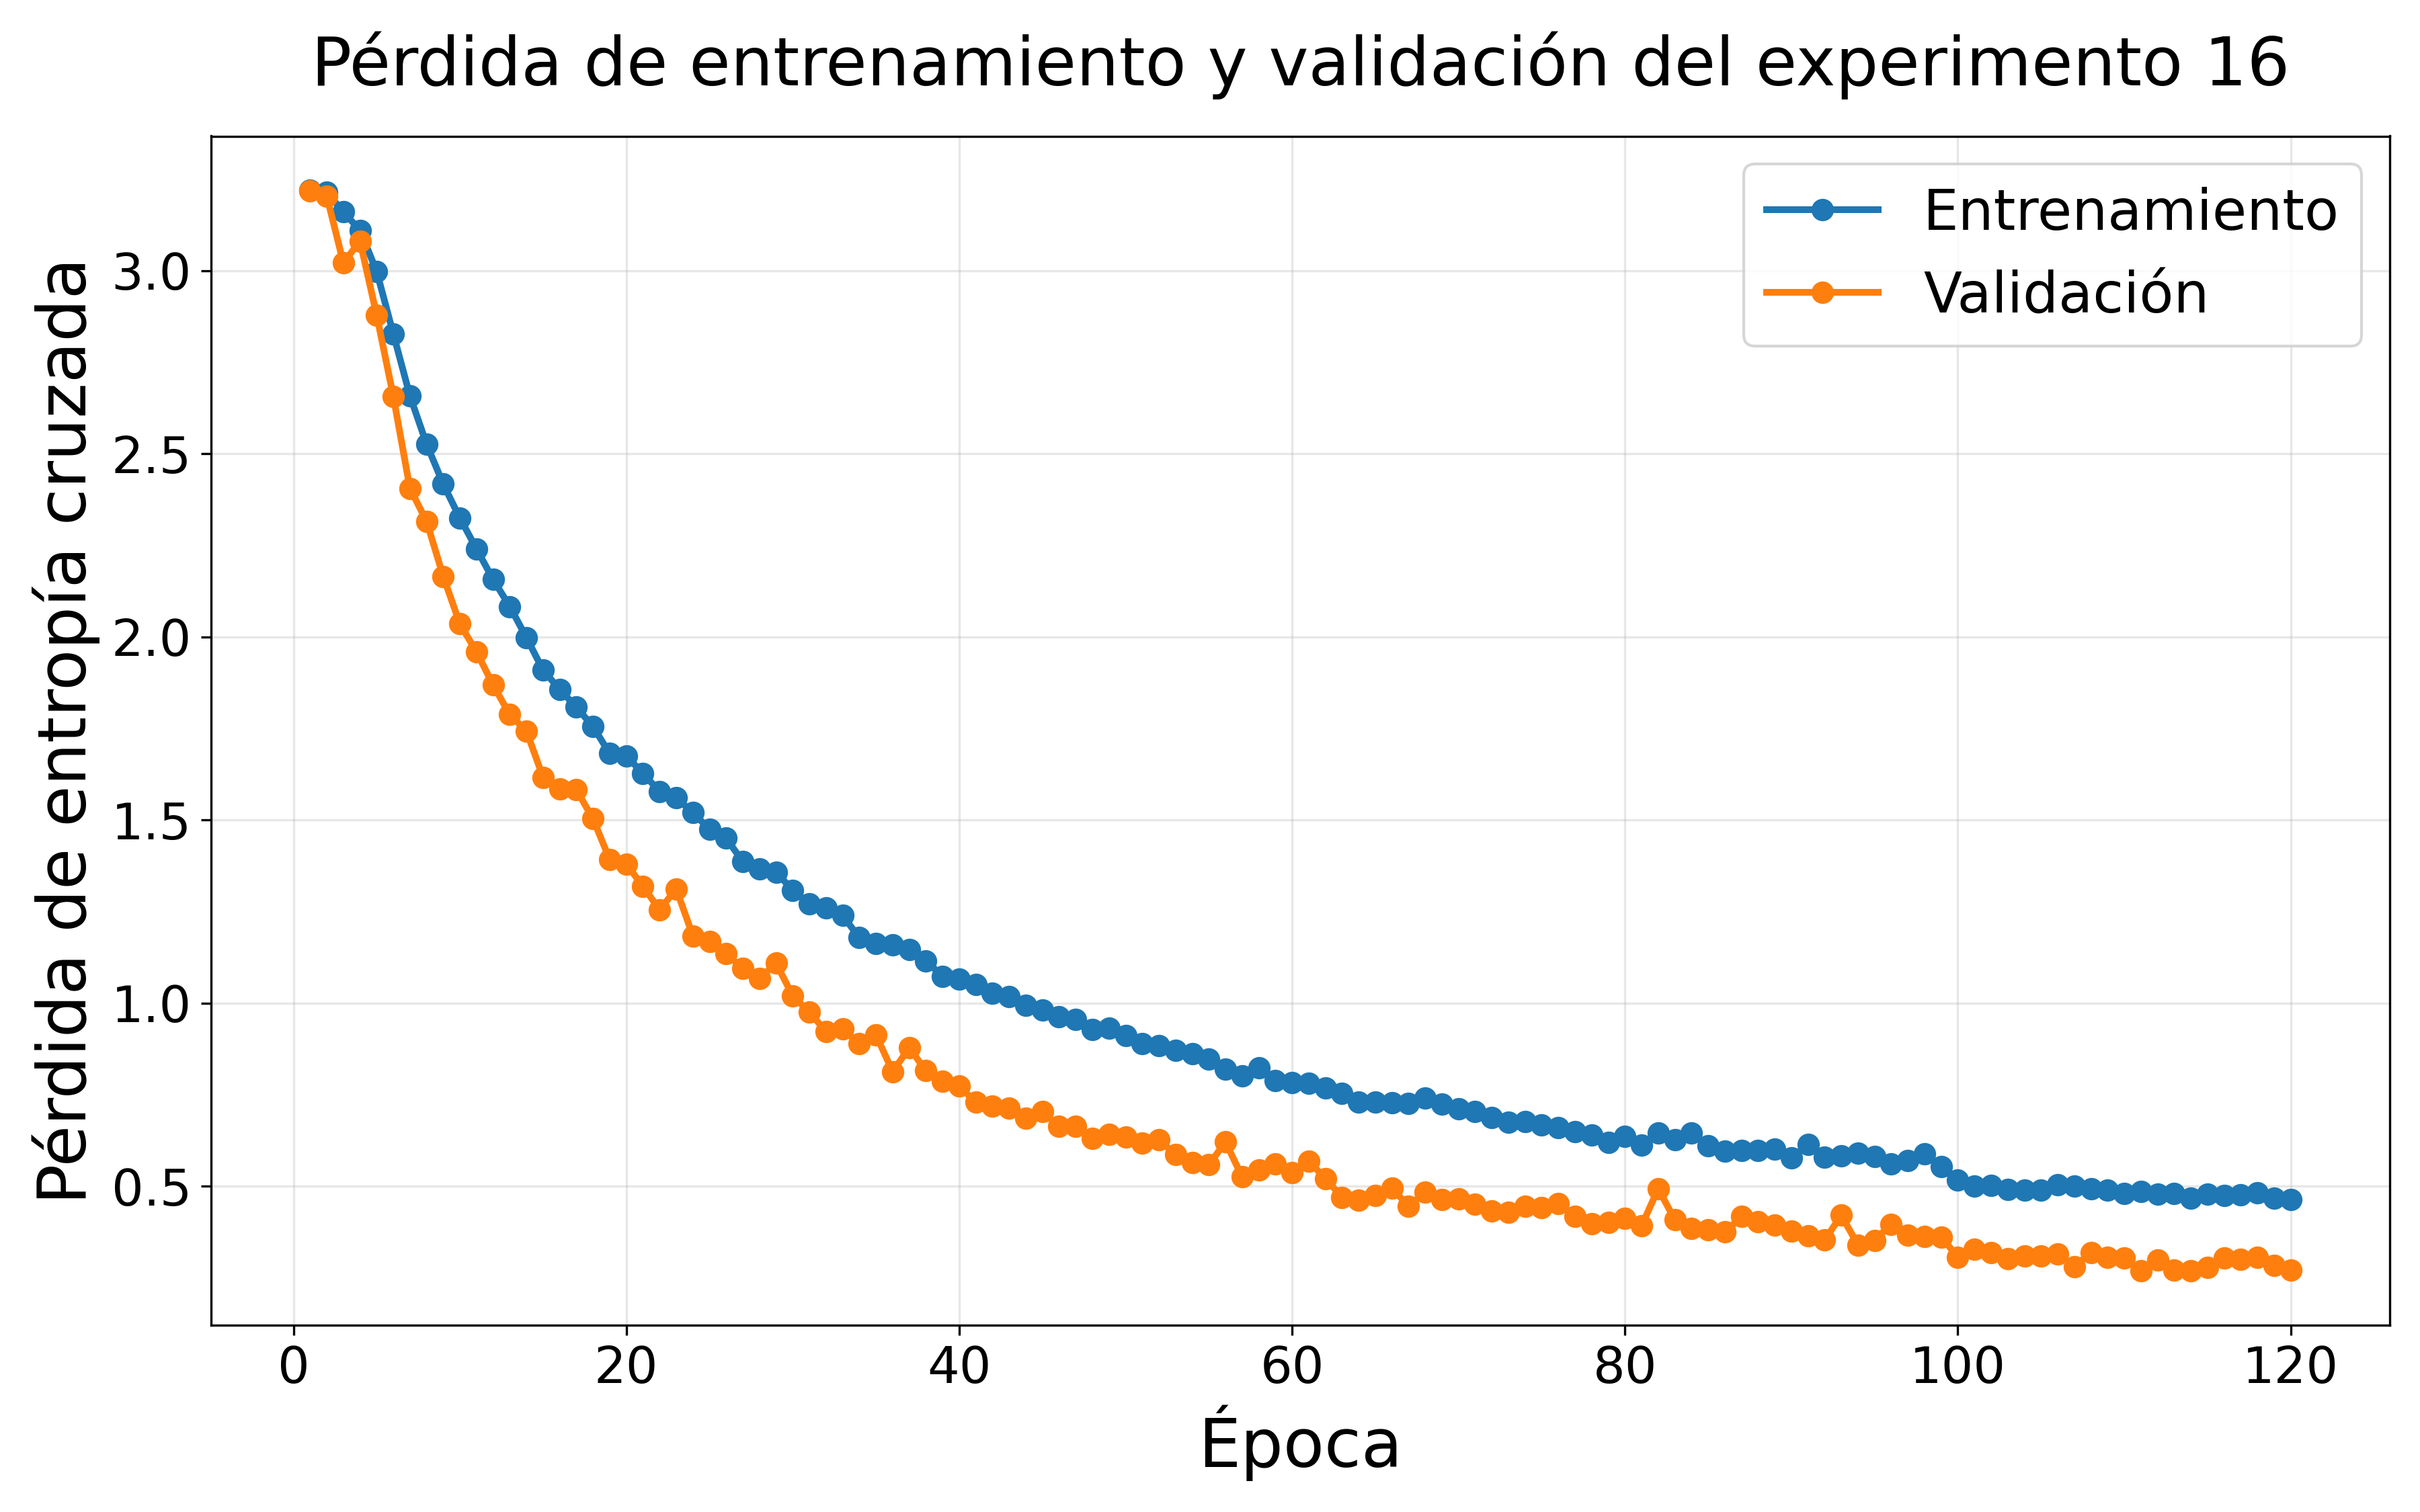
\includegraphics[width=\textwidth]{figures/Experiments_logs/loss_curve_05-14-1025.png}
        \caption{}
        \label{fig:loss_curve_05-14-1025}
    \end{subfigure}
    \hfill
    \begin{subfigure}{0.45\textwidth}
        \centering
        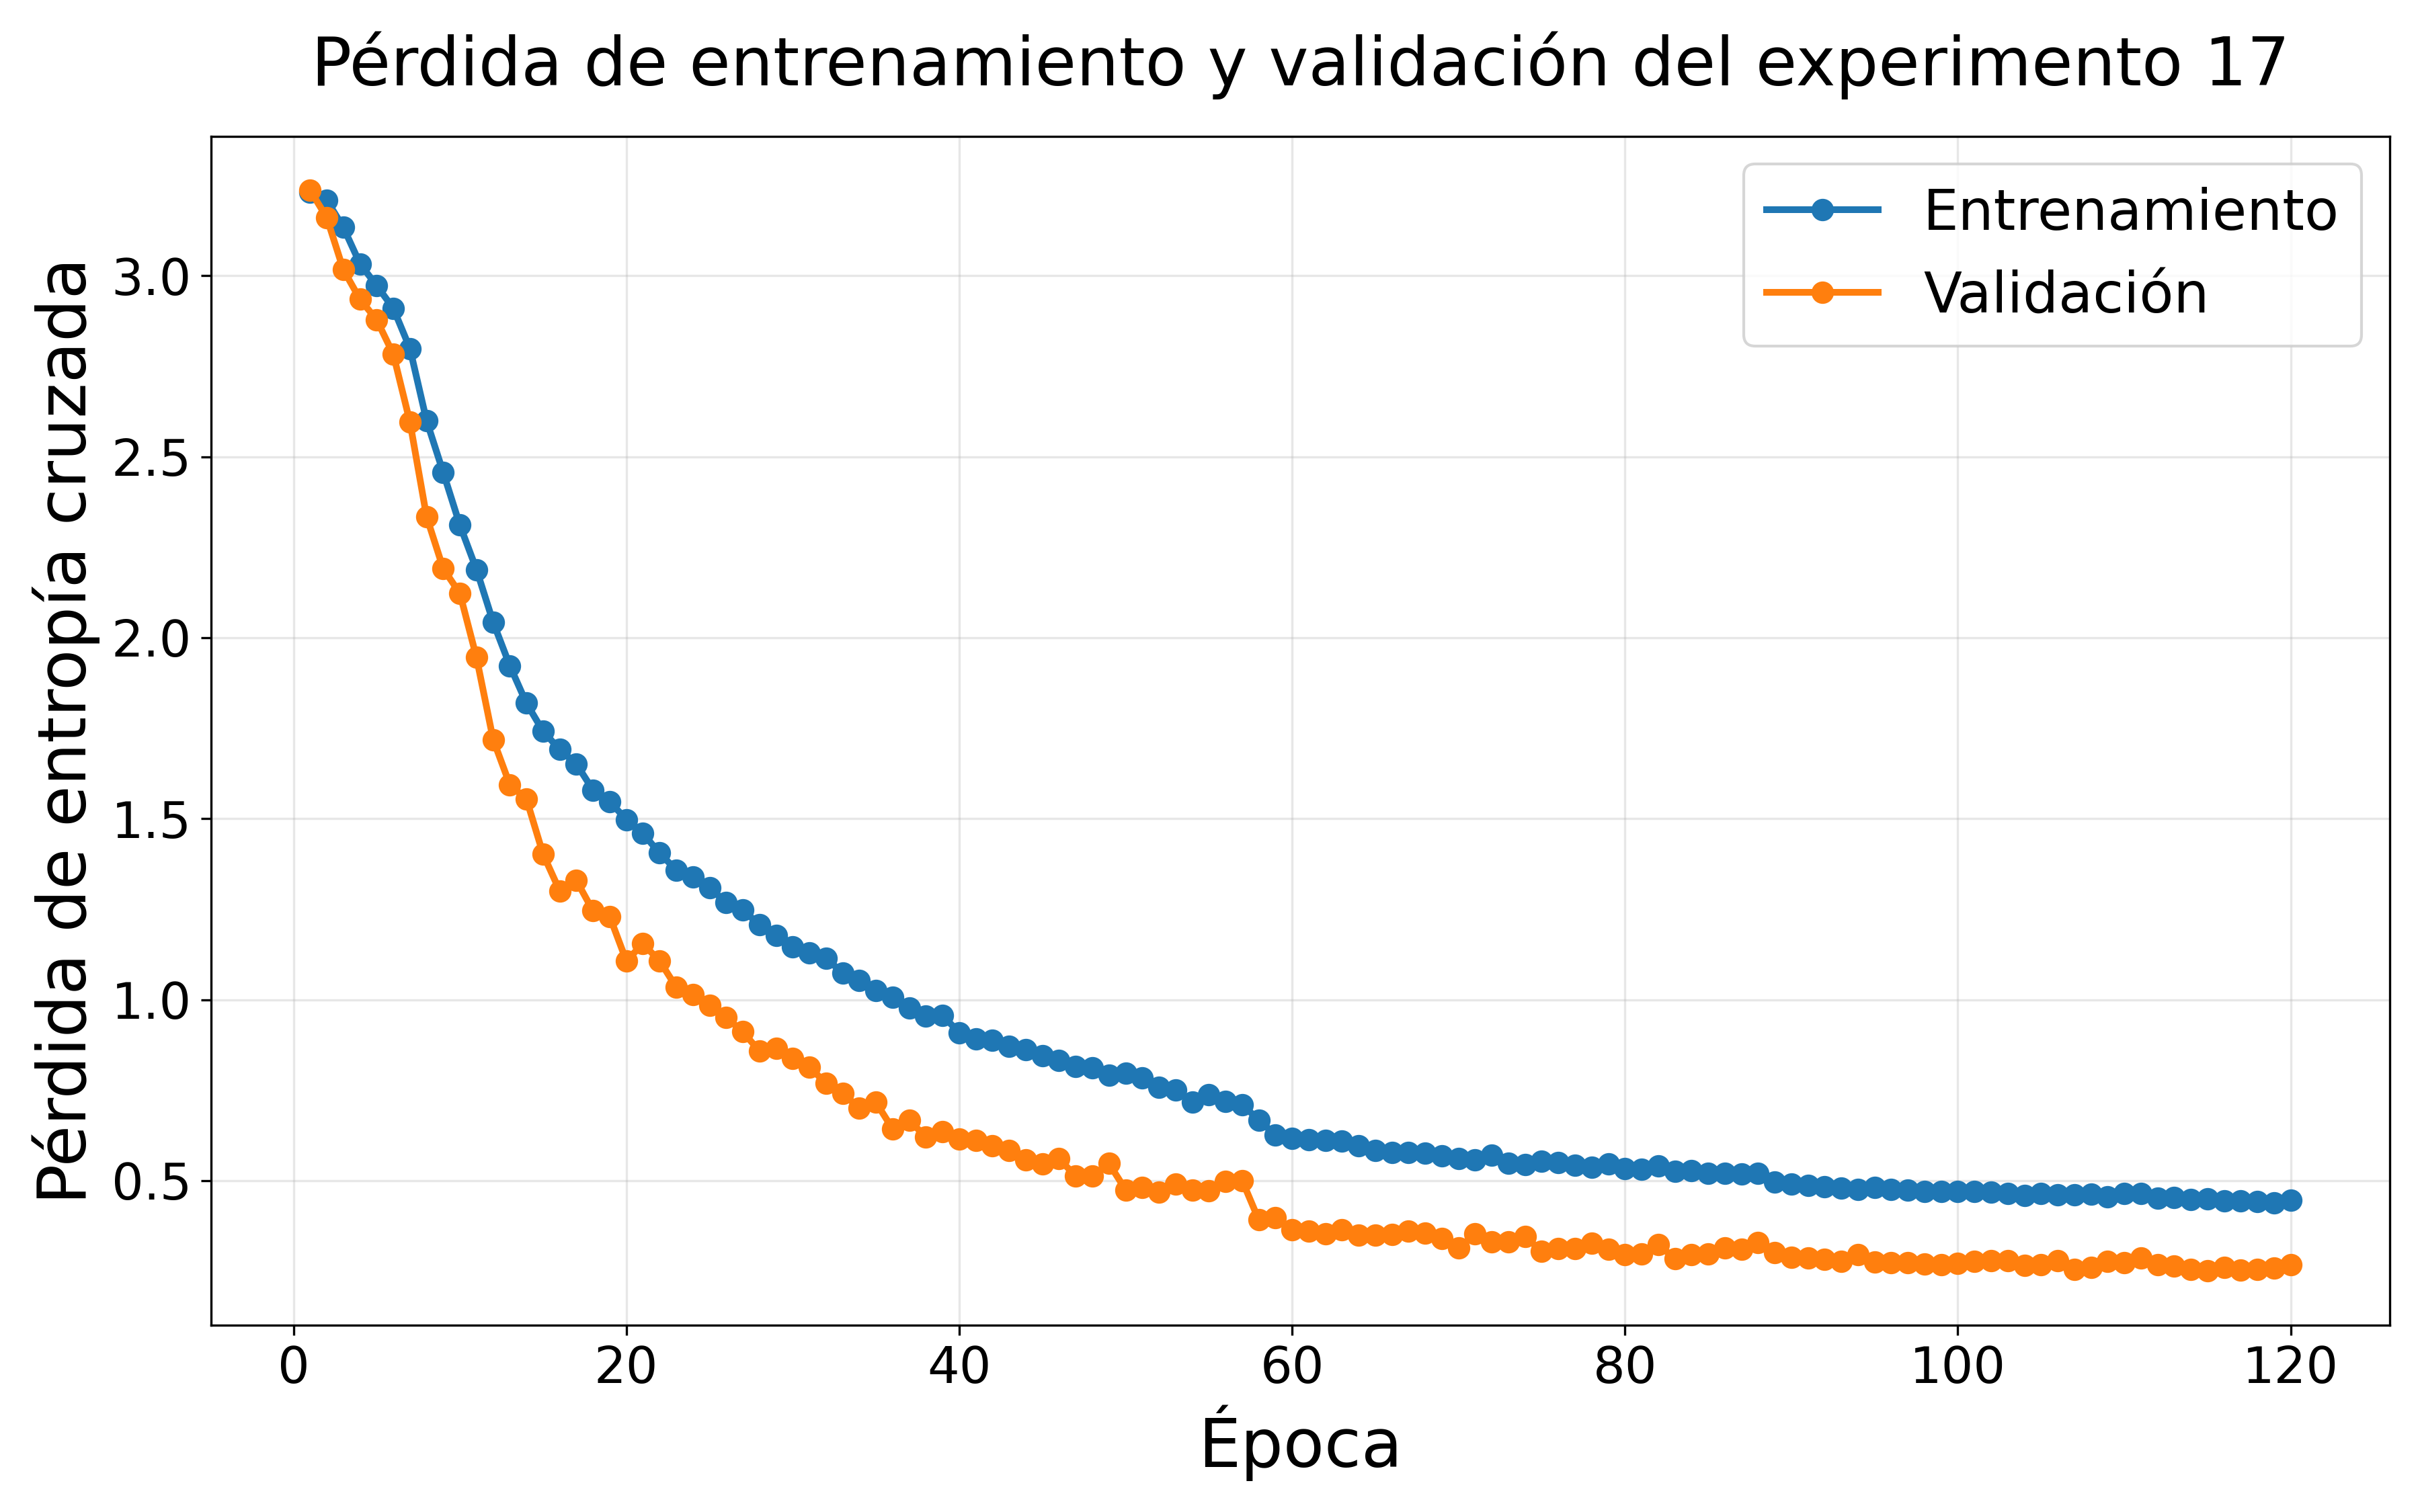
\includegraphics[width=\textwidth]{figures/Experiments_logs/loss_curve_05-14-1026.png}
        \caption{}
        \label{fig:loss_curve_05-14-1026}
    \end{subfigure}

    \vspace{0.4cm}

    \begin{subfigure}{0.45\textwidth}
        \centering
        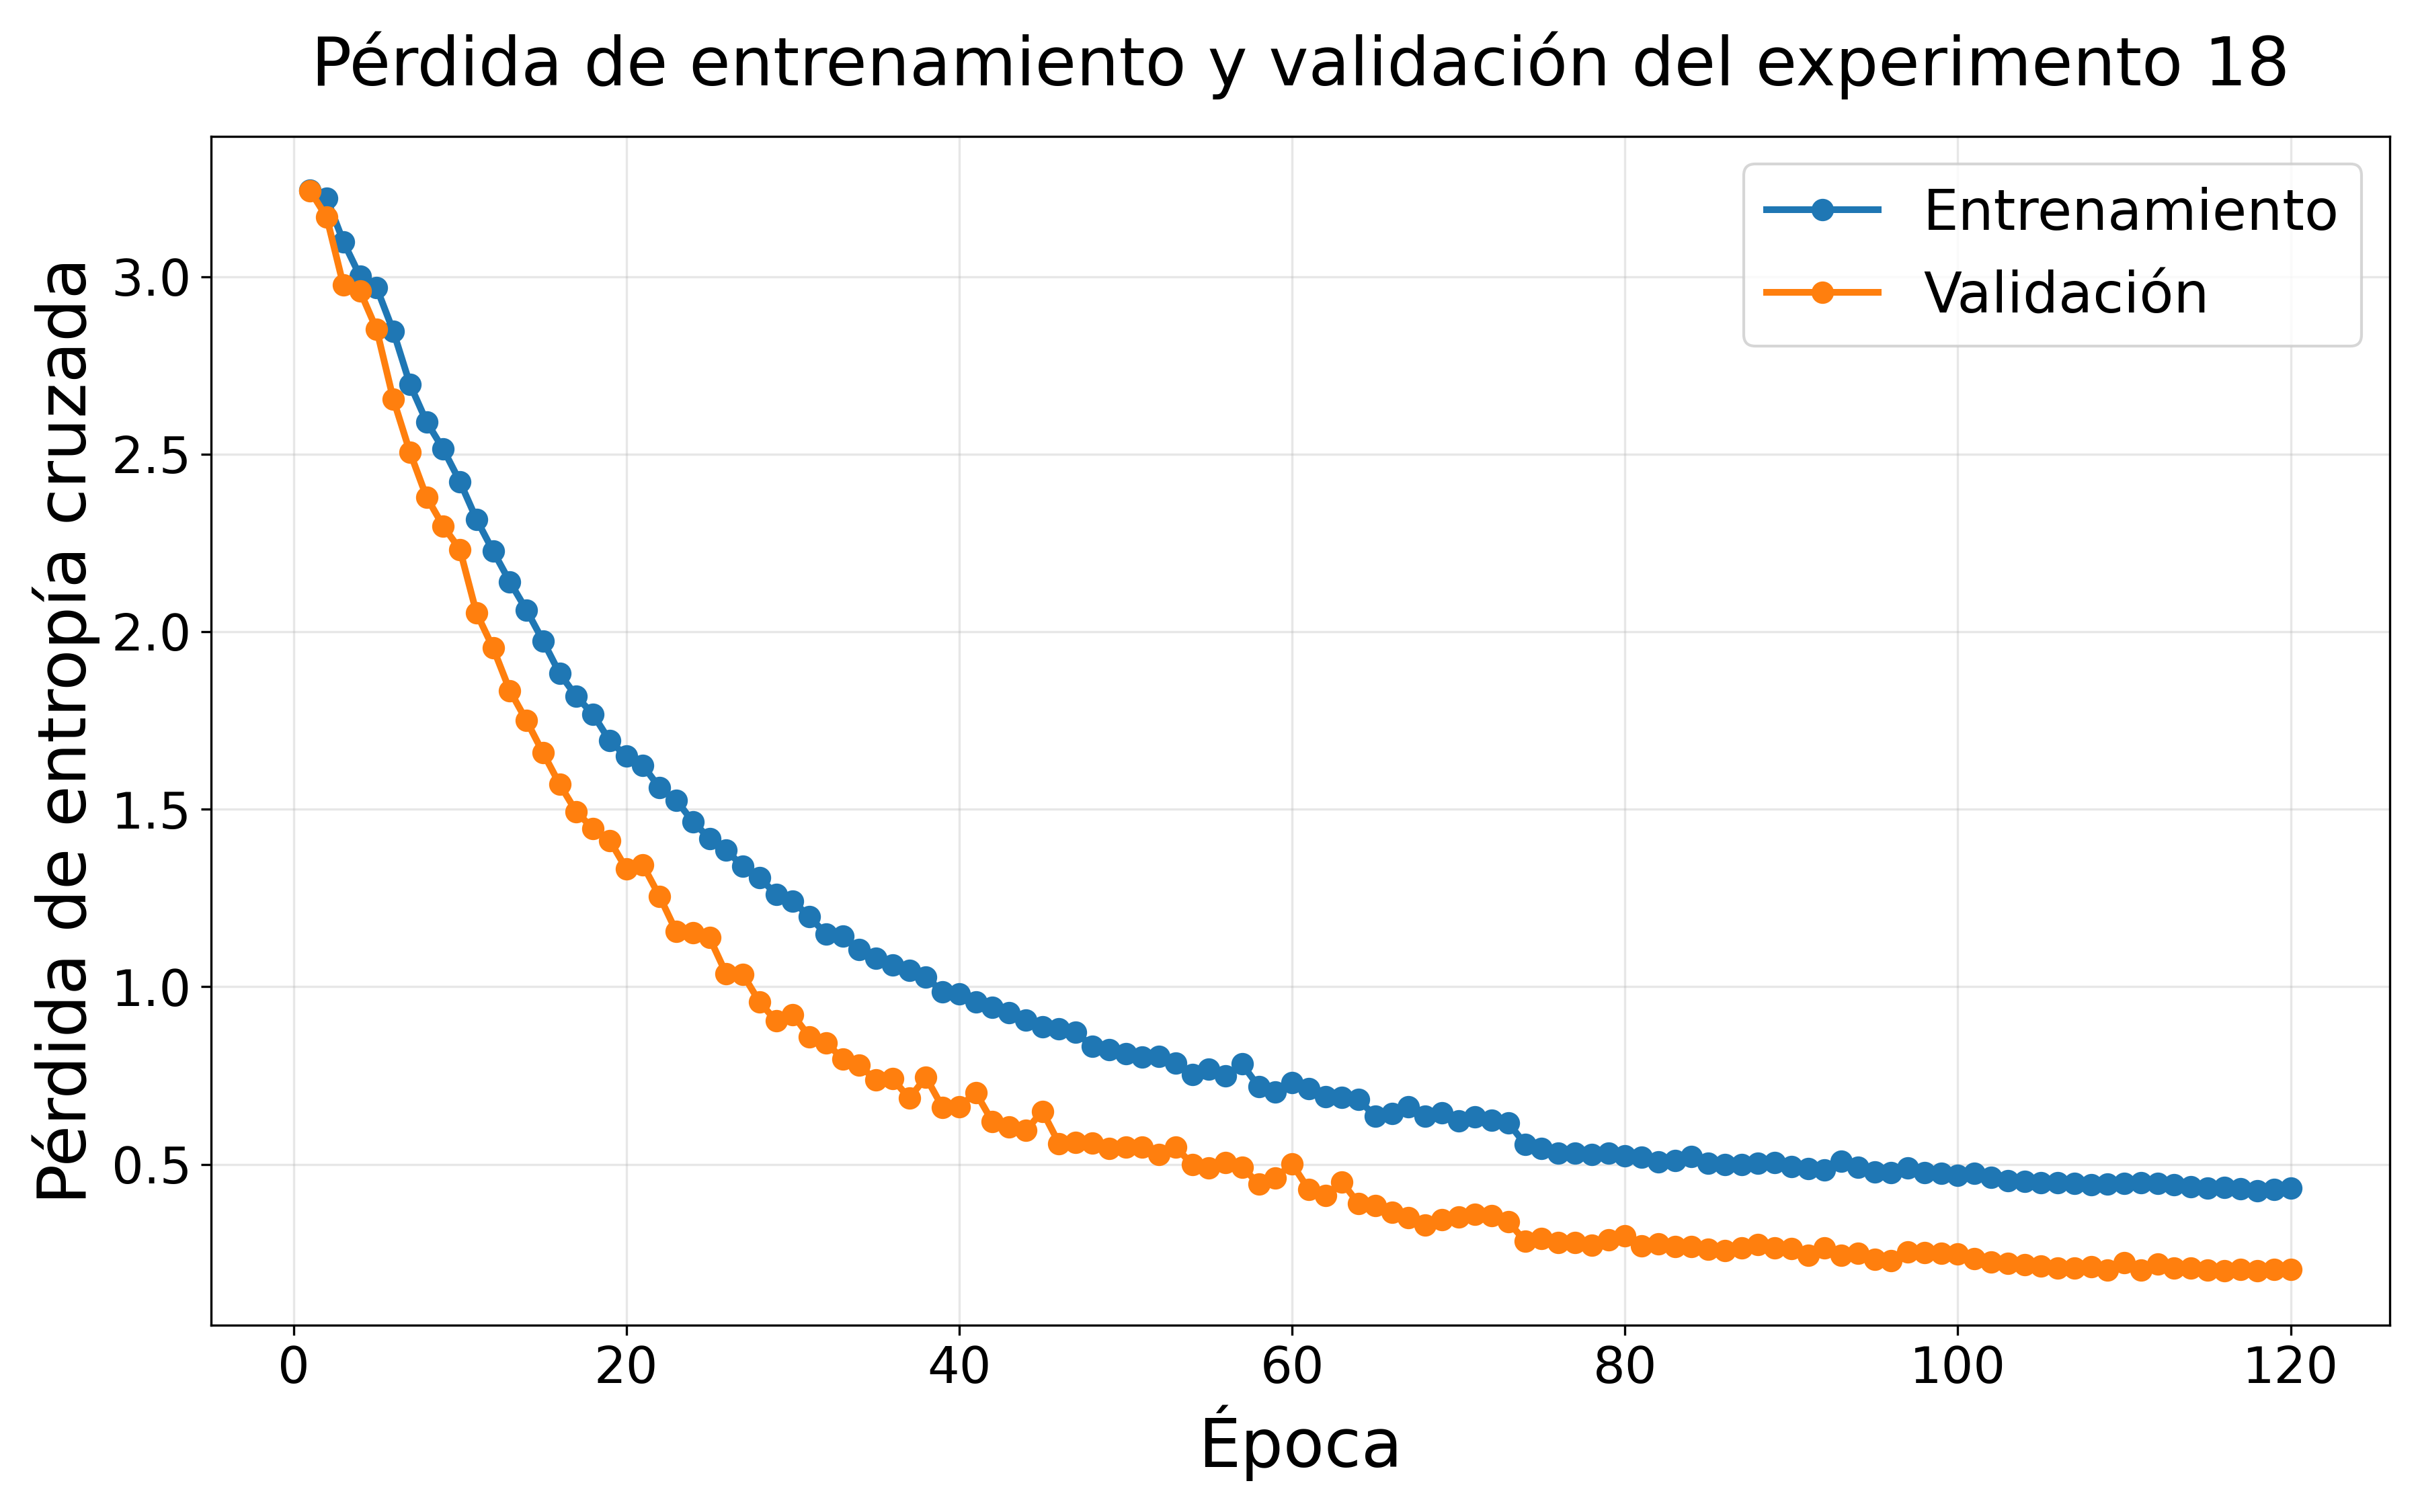
\includegraphics[width=\textwidth]{figures/Experiments_logs/loss_curve_05-14-1106.png}
        \caption{}
        \label{fig:loss_curve_05-14-1106}
    \end{subfigure}
    \hfill
    \begin{subfigure}{0.45\textwidth}
        \centering
        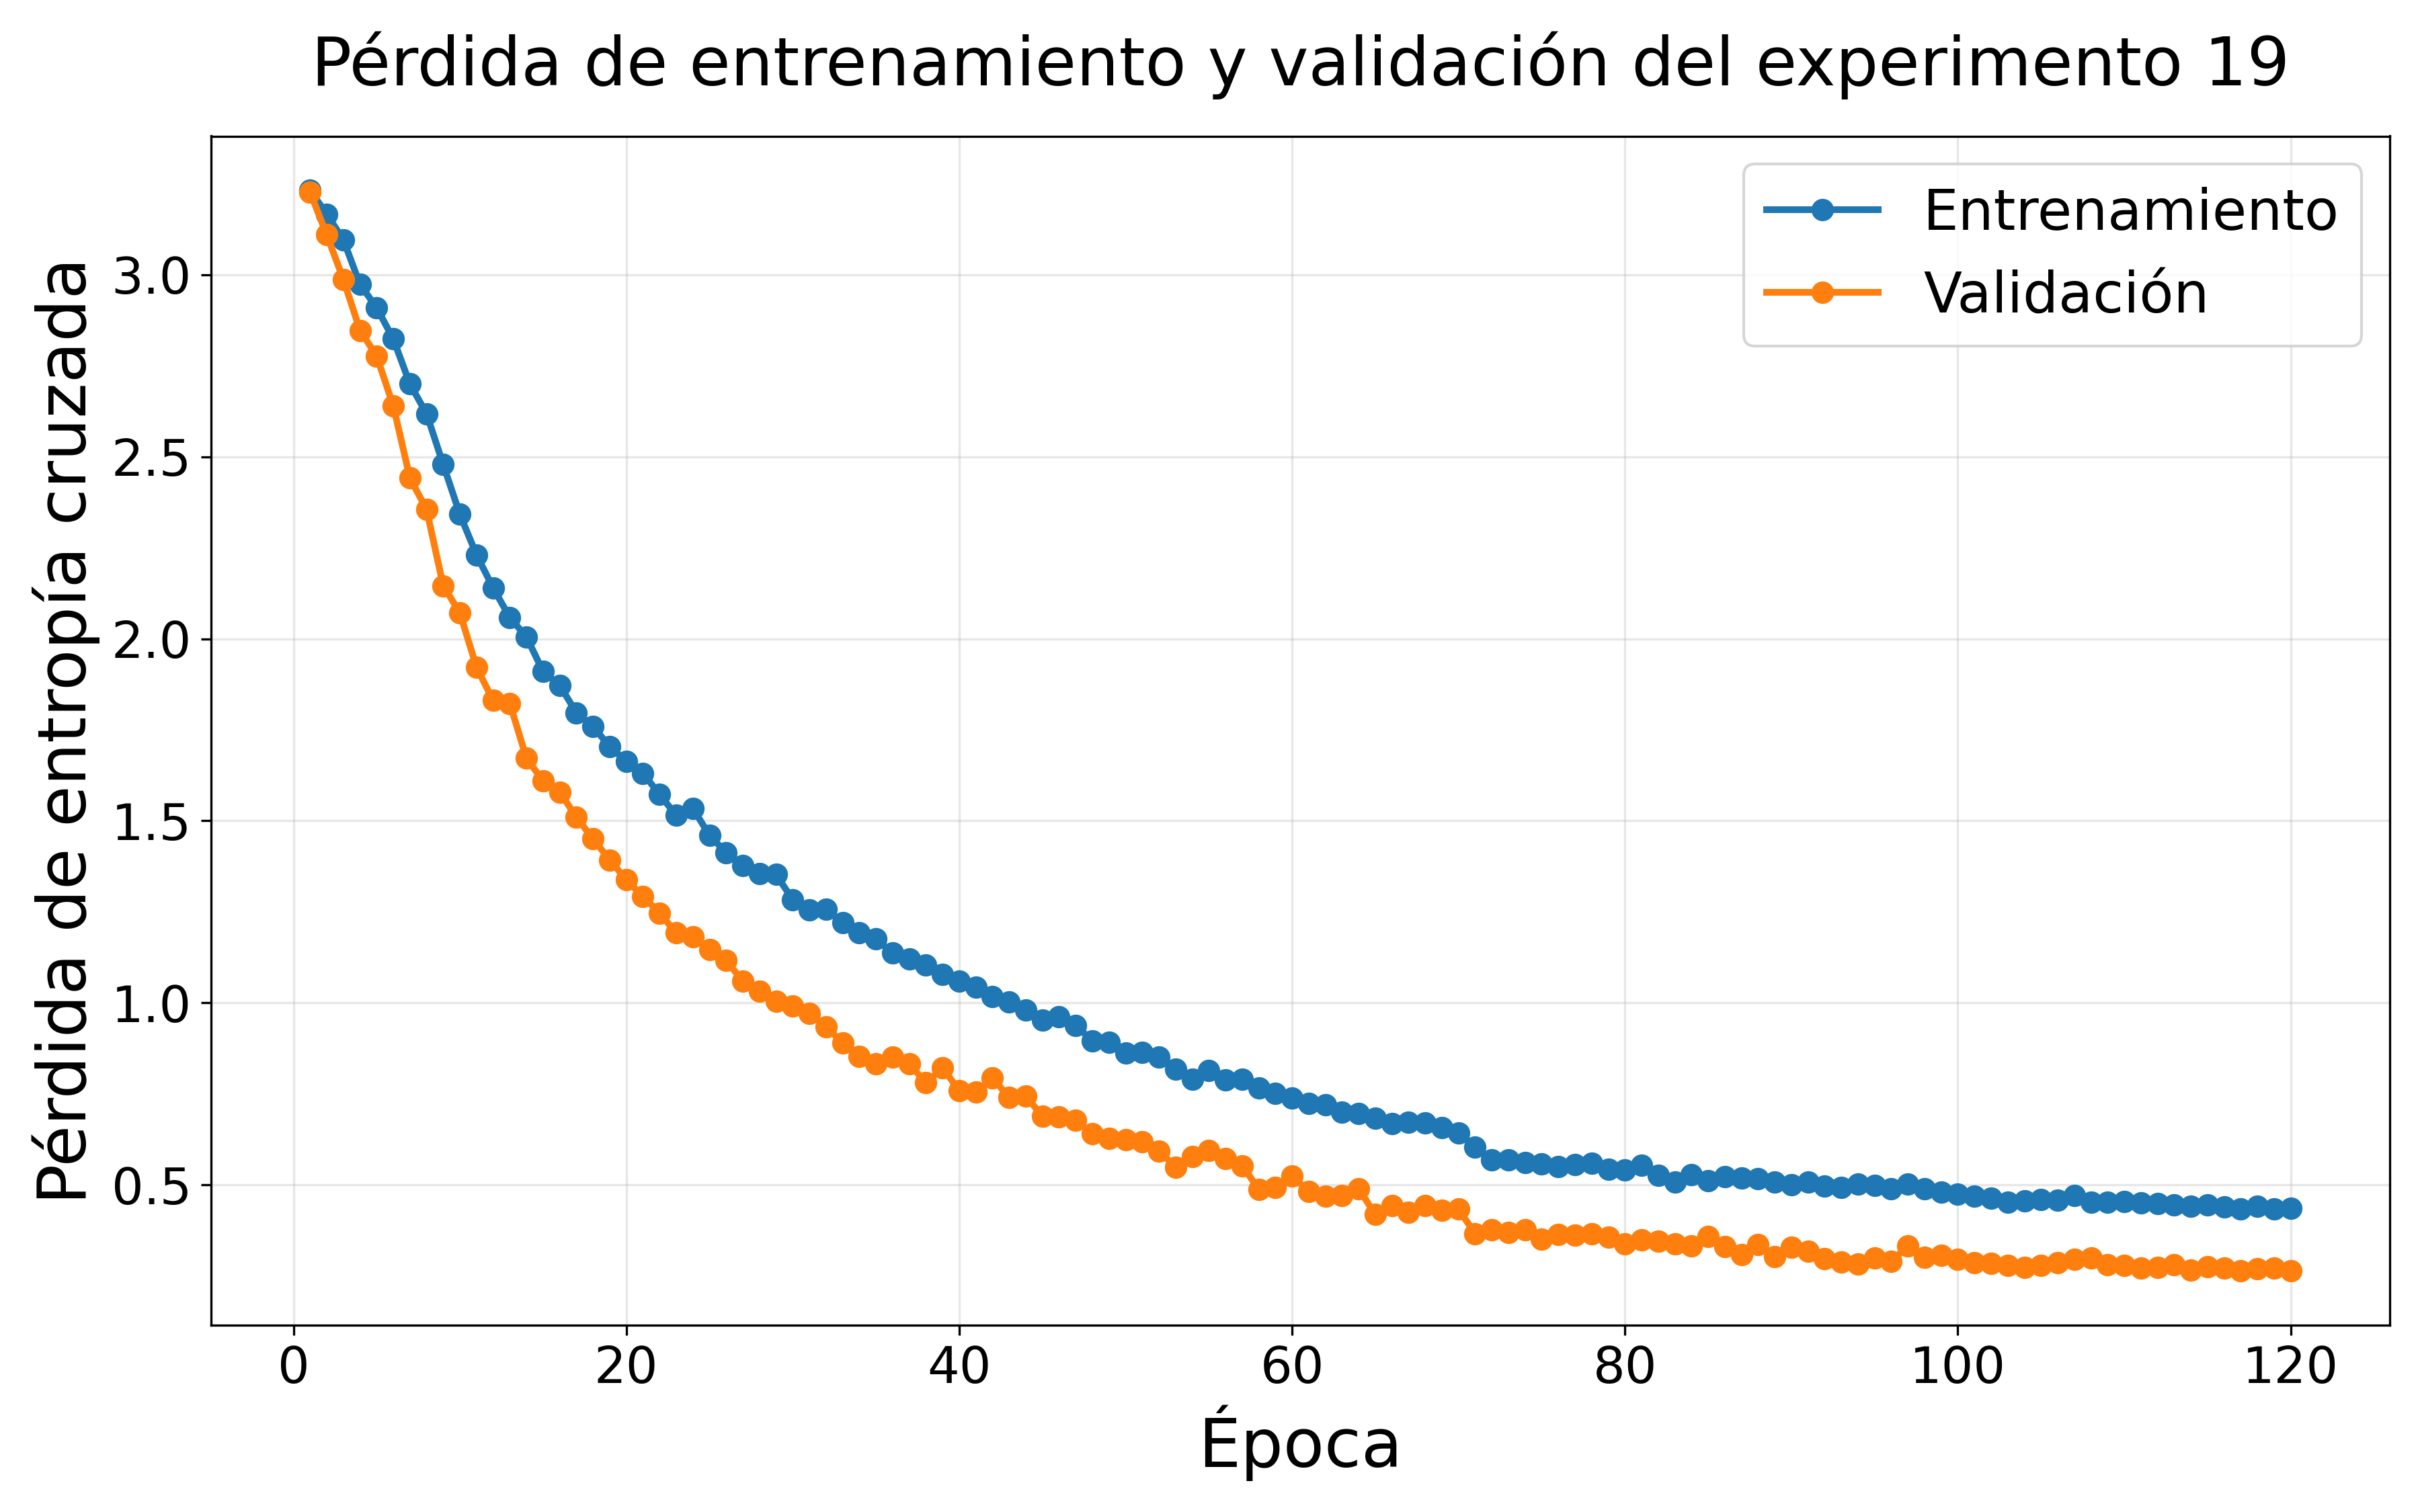
\includegraphics[width=\textwidth]{figures/Experiments_logs/loss_curve_05-14-1107.png}
        \caption{}
        \label{fig:loss_curve_05-14-1107}
    \end{subfigure}

    \caption{Experimentos realizados con el cambio del \textit{data augmentation}}
    \label{fig:loss_curve_05-14}
\end{figure}

Este fue el salto más grande del proyecto. Antes de esta modificación, el mejor resultado estaba alrededor de 88,94\%. Con \textit{data augmentation light}, los cuatro experimentos superaron el 94\%, y la mejor llegó a 96,05\%. Estos resultados confirman las hipótesis 4; la preparación de datos y la regularización visual fueron decisivas.

\section{Mejor modelo obtenido}

El experimento con mejores resultados es el número 18. La configuración principal fue la siguiente. \textit{Seed} 69, dimensión 12/12, embedding AIM, \texttt{HybridCustomTTN}, cabeza lineal, \textit{learning rate} 0,00025, warmup coseno de 5 épocas, label smoothing 0,05, regularización $L_2$ suave, preservación de relación de aspecto y aumento de datos \texttt{light}.

\begin{table}[H]
\centering
\small
\begin{tabular}{lc}
\toprule
\textbf{Métrica} & \textbf{Valor} \\
\midrule
Accuracy top-1 & 96,05\% \\
Accuracy top-5 & 99,43\% \\
Macro precision & 96,12\% \\
Macro recall & 95,82\% \\
Macro F1 & 95,94\% \\
Weighted F1 & 96,05\% \\
\texttt{classification\_mAP} & 98,41\% \\
Eval loss final & 0,2037 \\
\bottomrule
\end{tabular}
\caption{Métricas principales del mejor modelo sobre ChemEq25.}
\label{tab:mejor_modelo}
\end{table}

\begin{figure}[htbp]
    \centering

    \begin{subfigure}{0.45\textwidth}
        \centering
        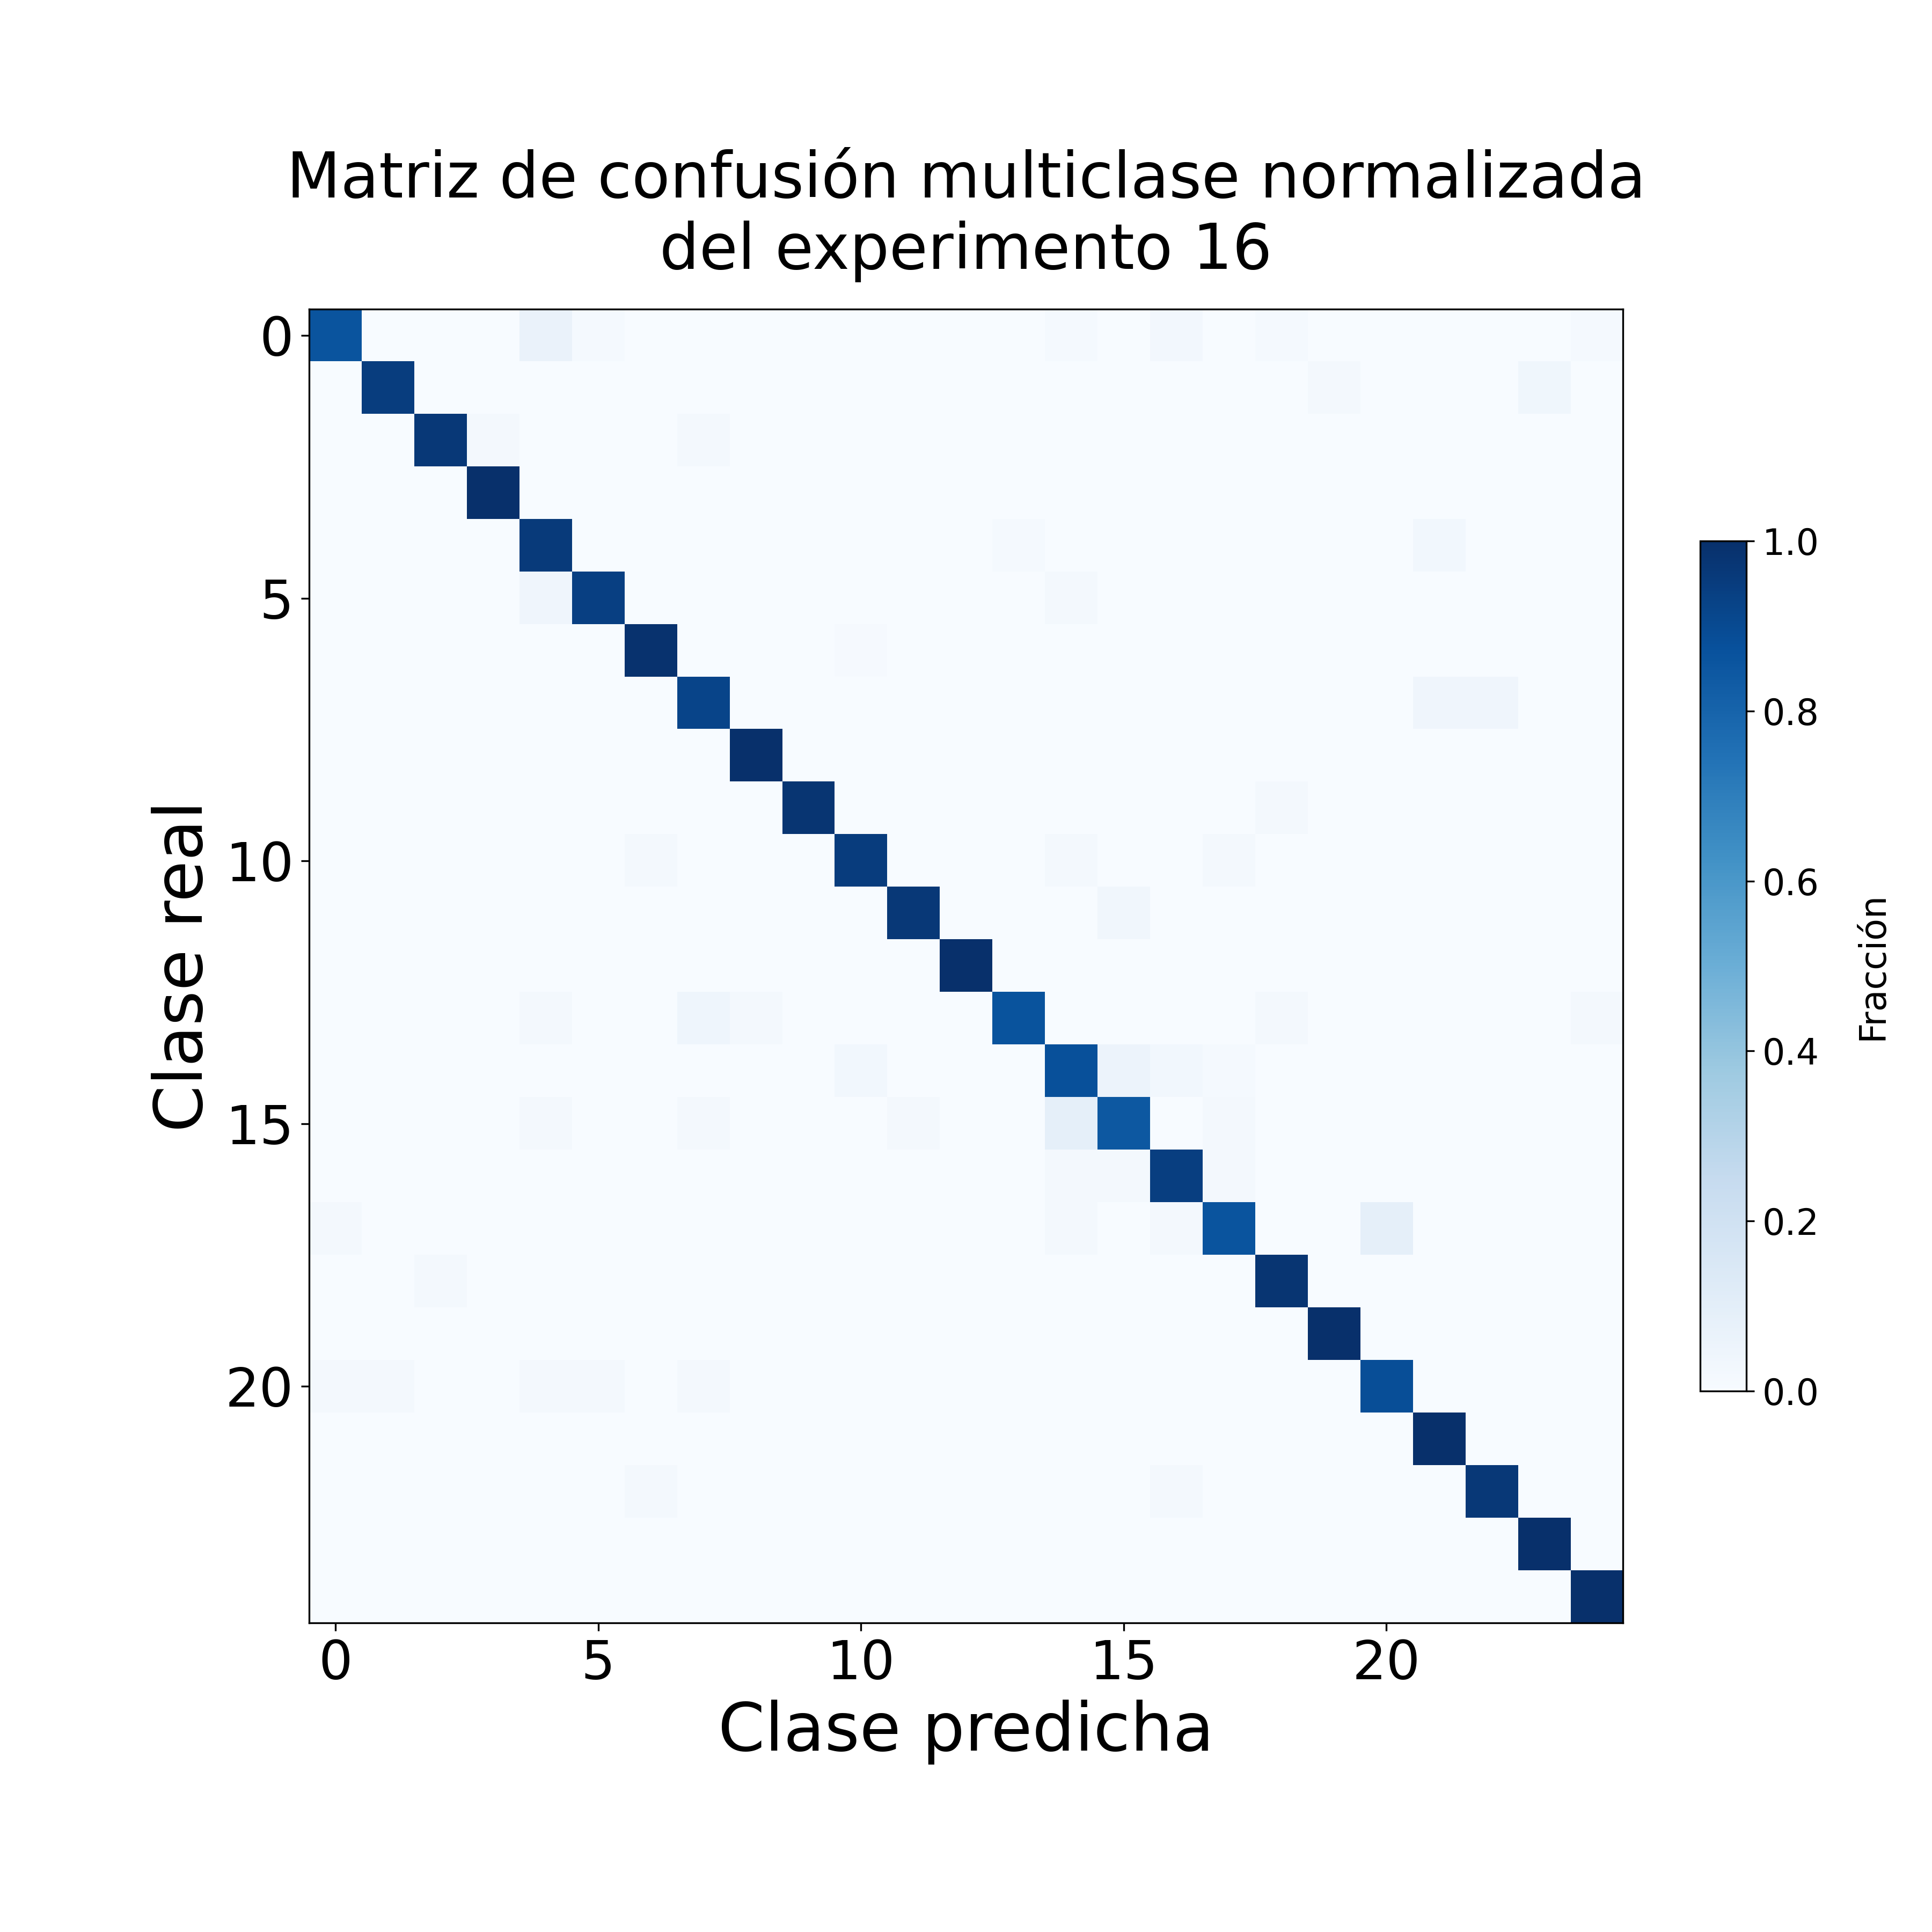
\includegraphics[width=\textwidth]{figures/Experiments_logs/confusion_matrix_05-14-1025.png}
        \caption{}
        \label{fig:confusion_matrix_05-14-1025}
    \end{subfigure}
    \hfill
    \begin{subfigure}{0.45\textwidth}
        \centering
        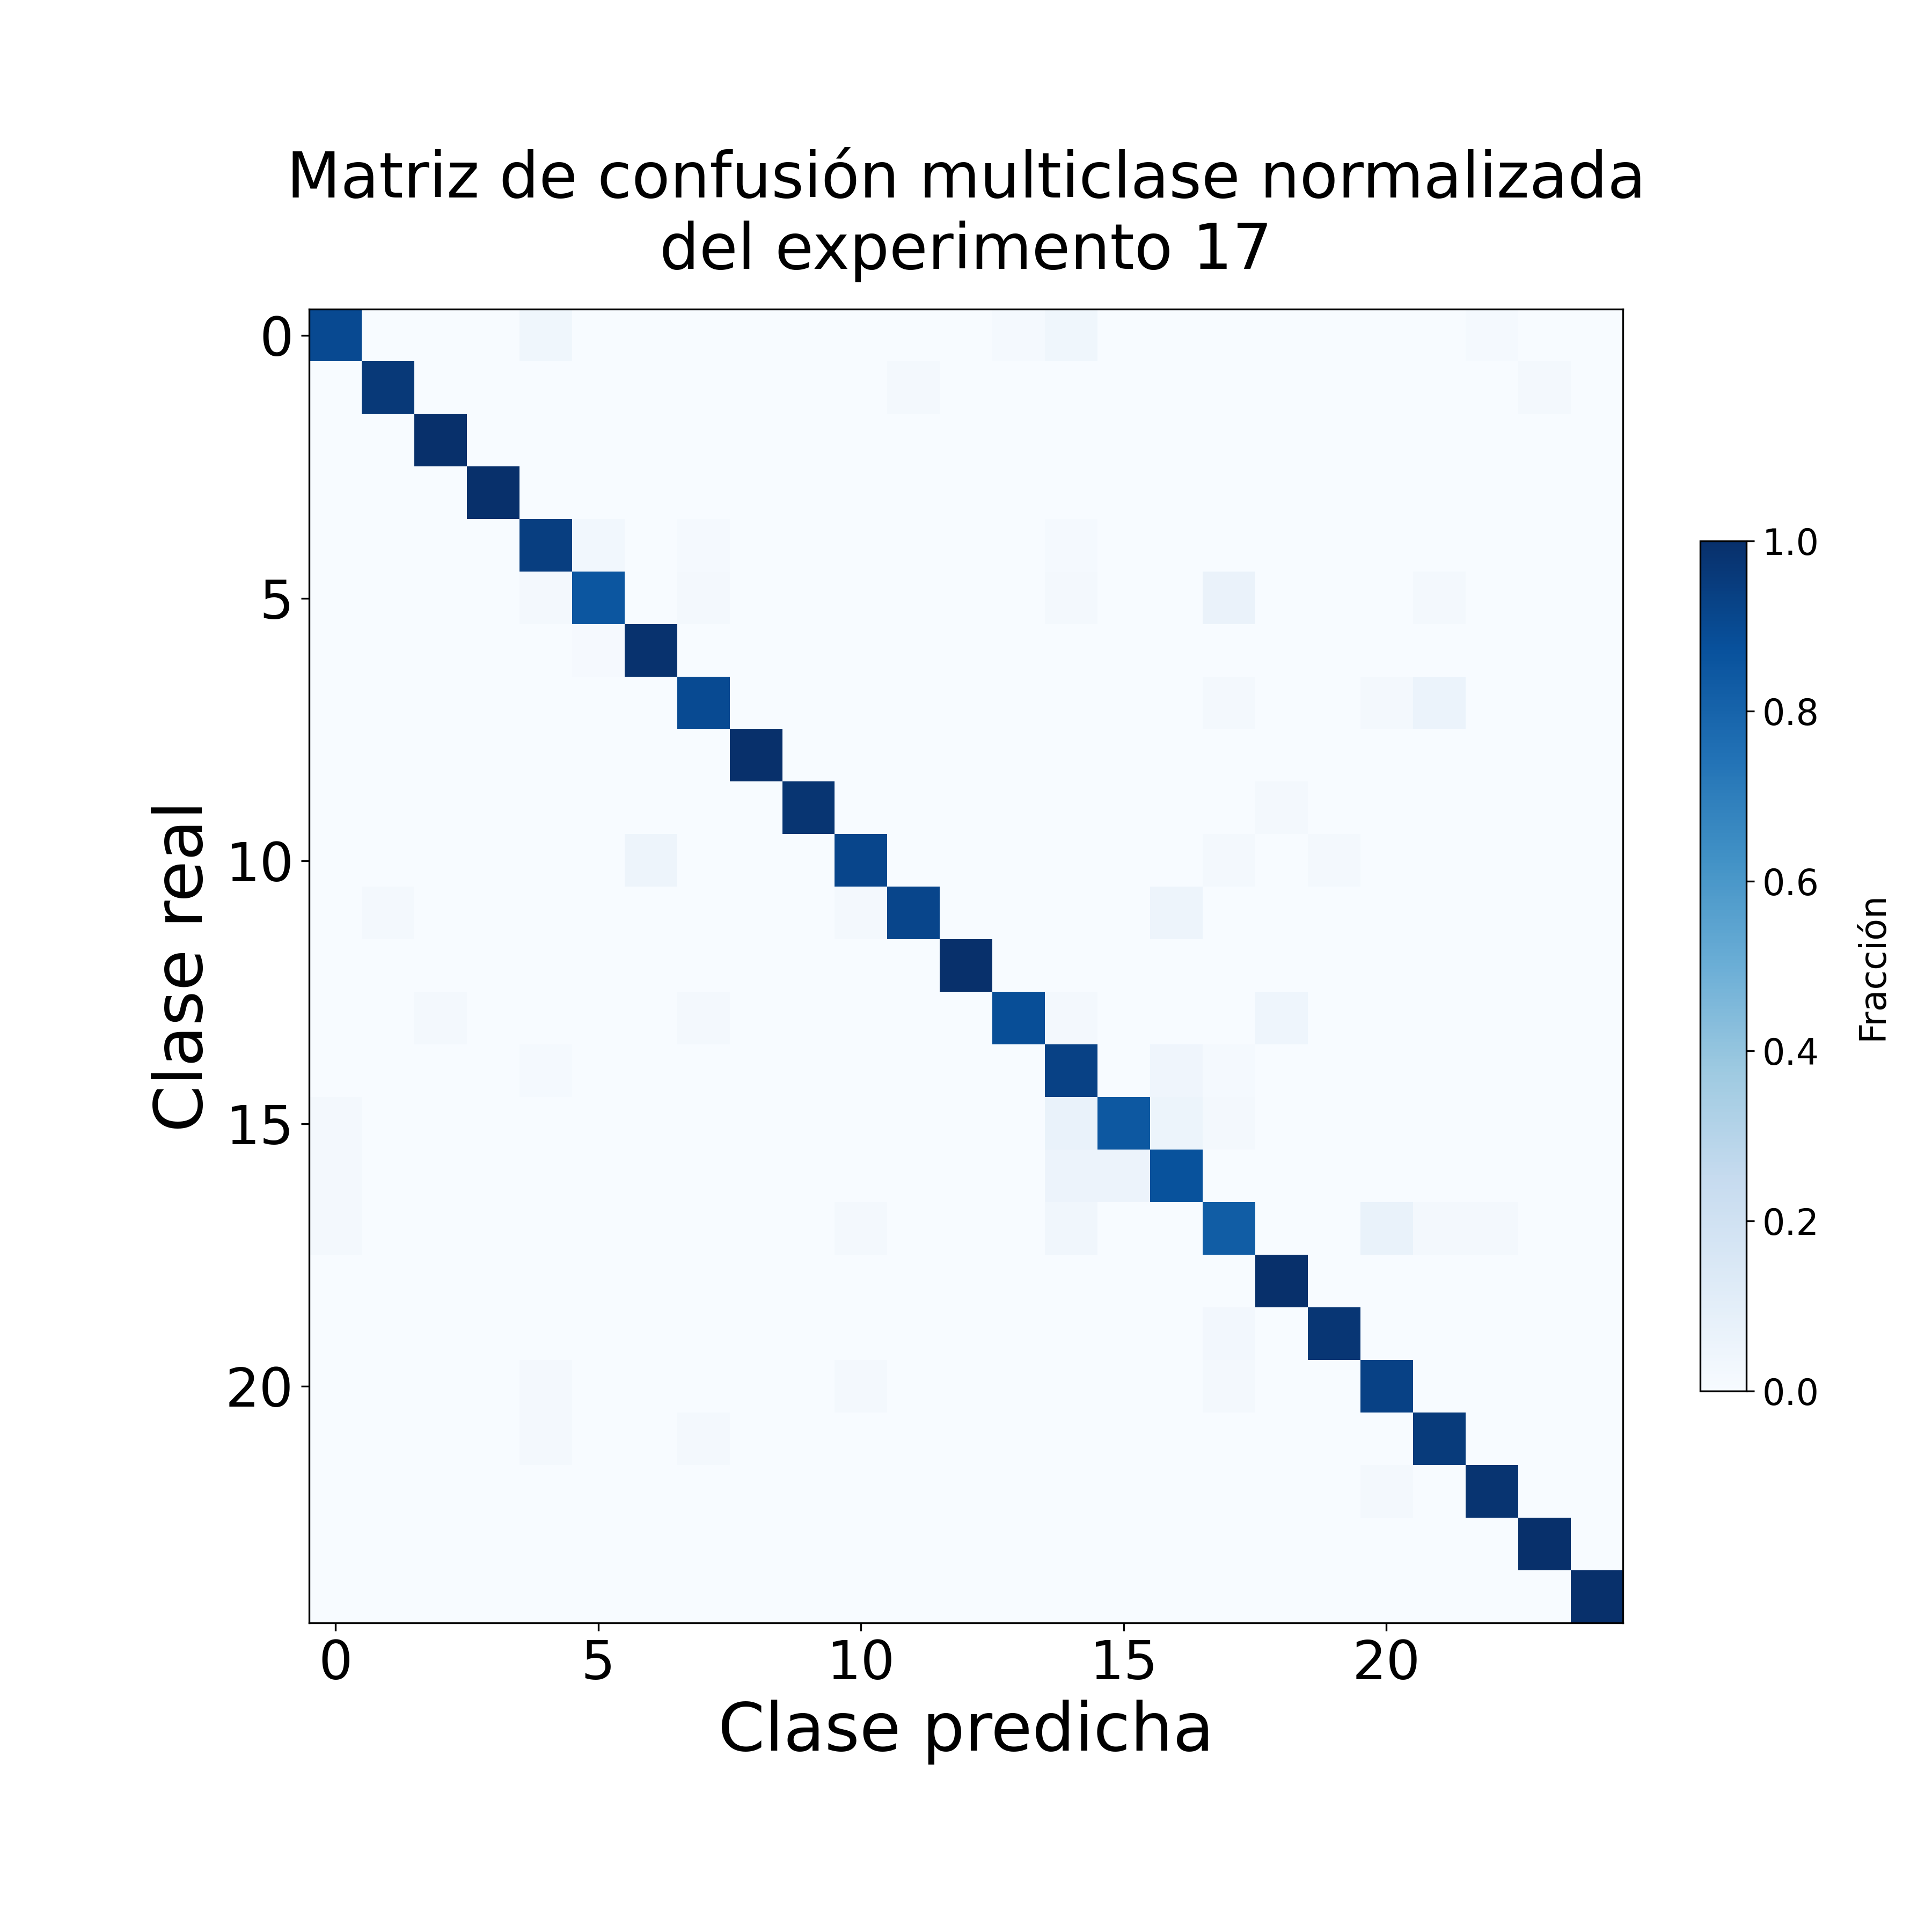
\includegraphics[width=\textwidth]{figures/Experiments_logs/confusion_matrix_05-14-1026.png}
        \caption{}
        \label{fig:confusion_matrix_05-14-1026}
    \end{subfigure}

    \vspace{0.4cm}

    \begin{subfigure}{0.45\textwidth}
        \centering
        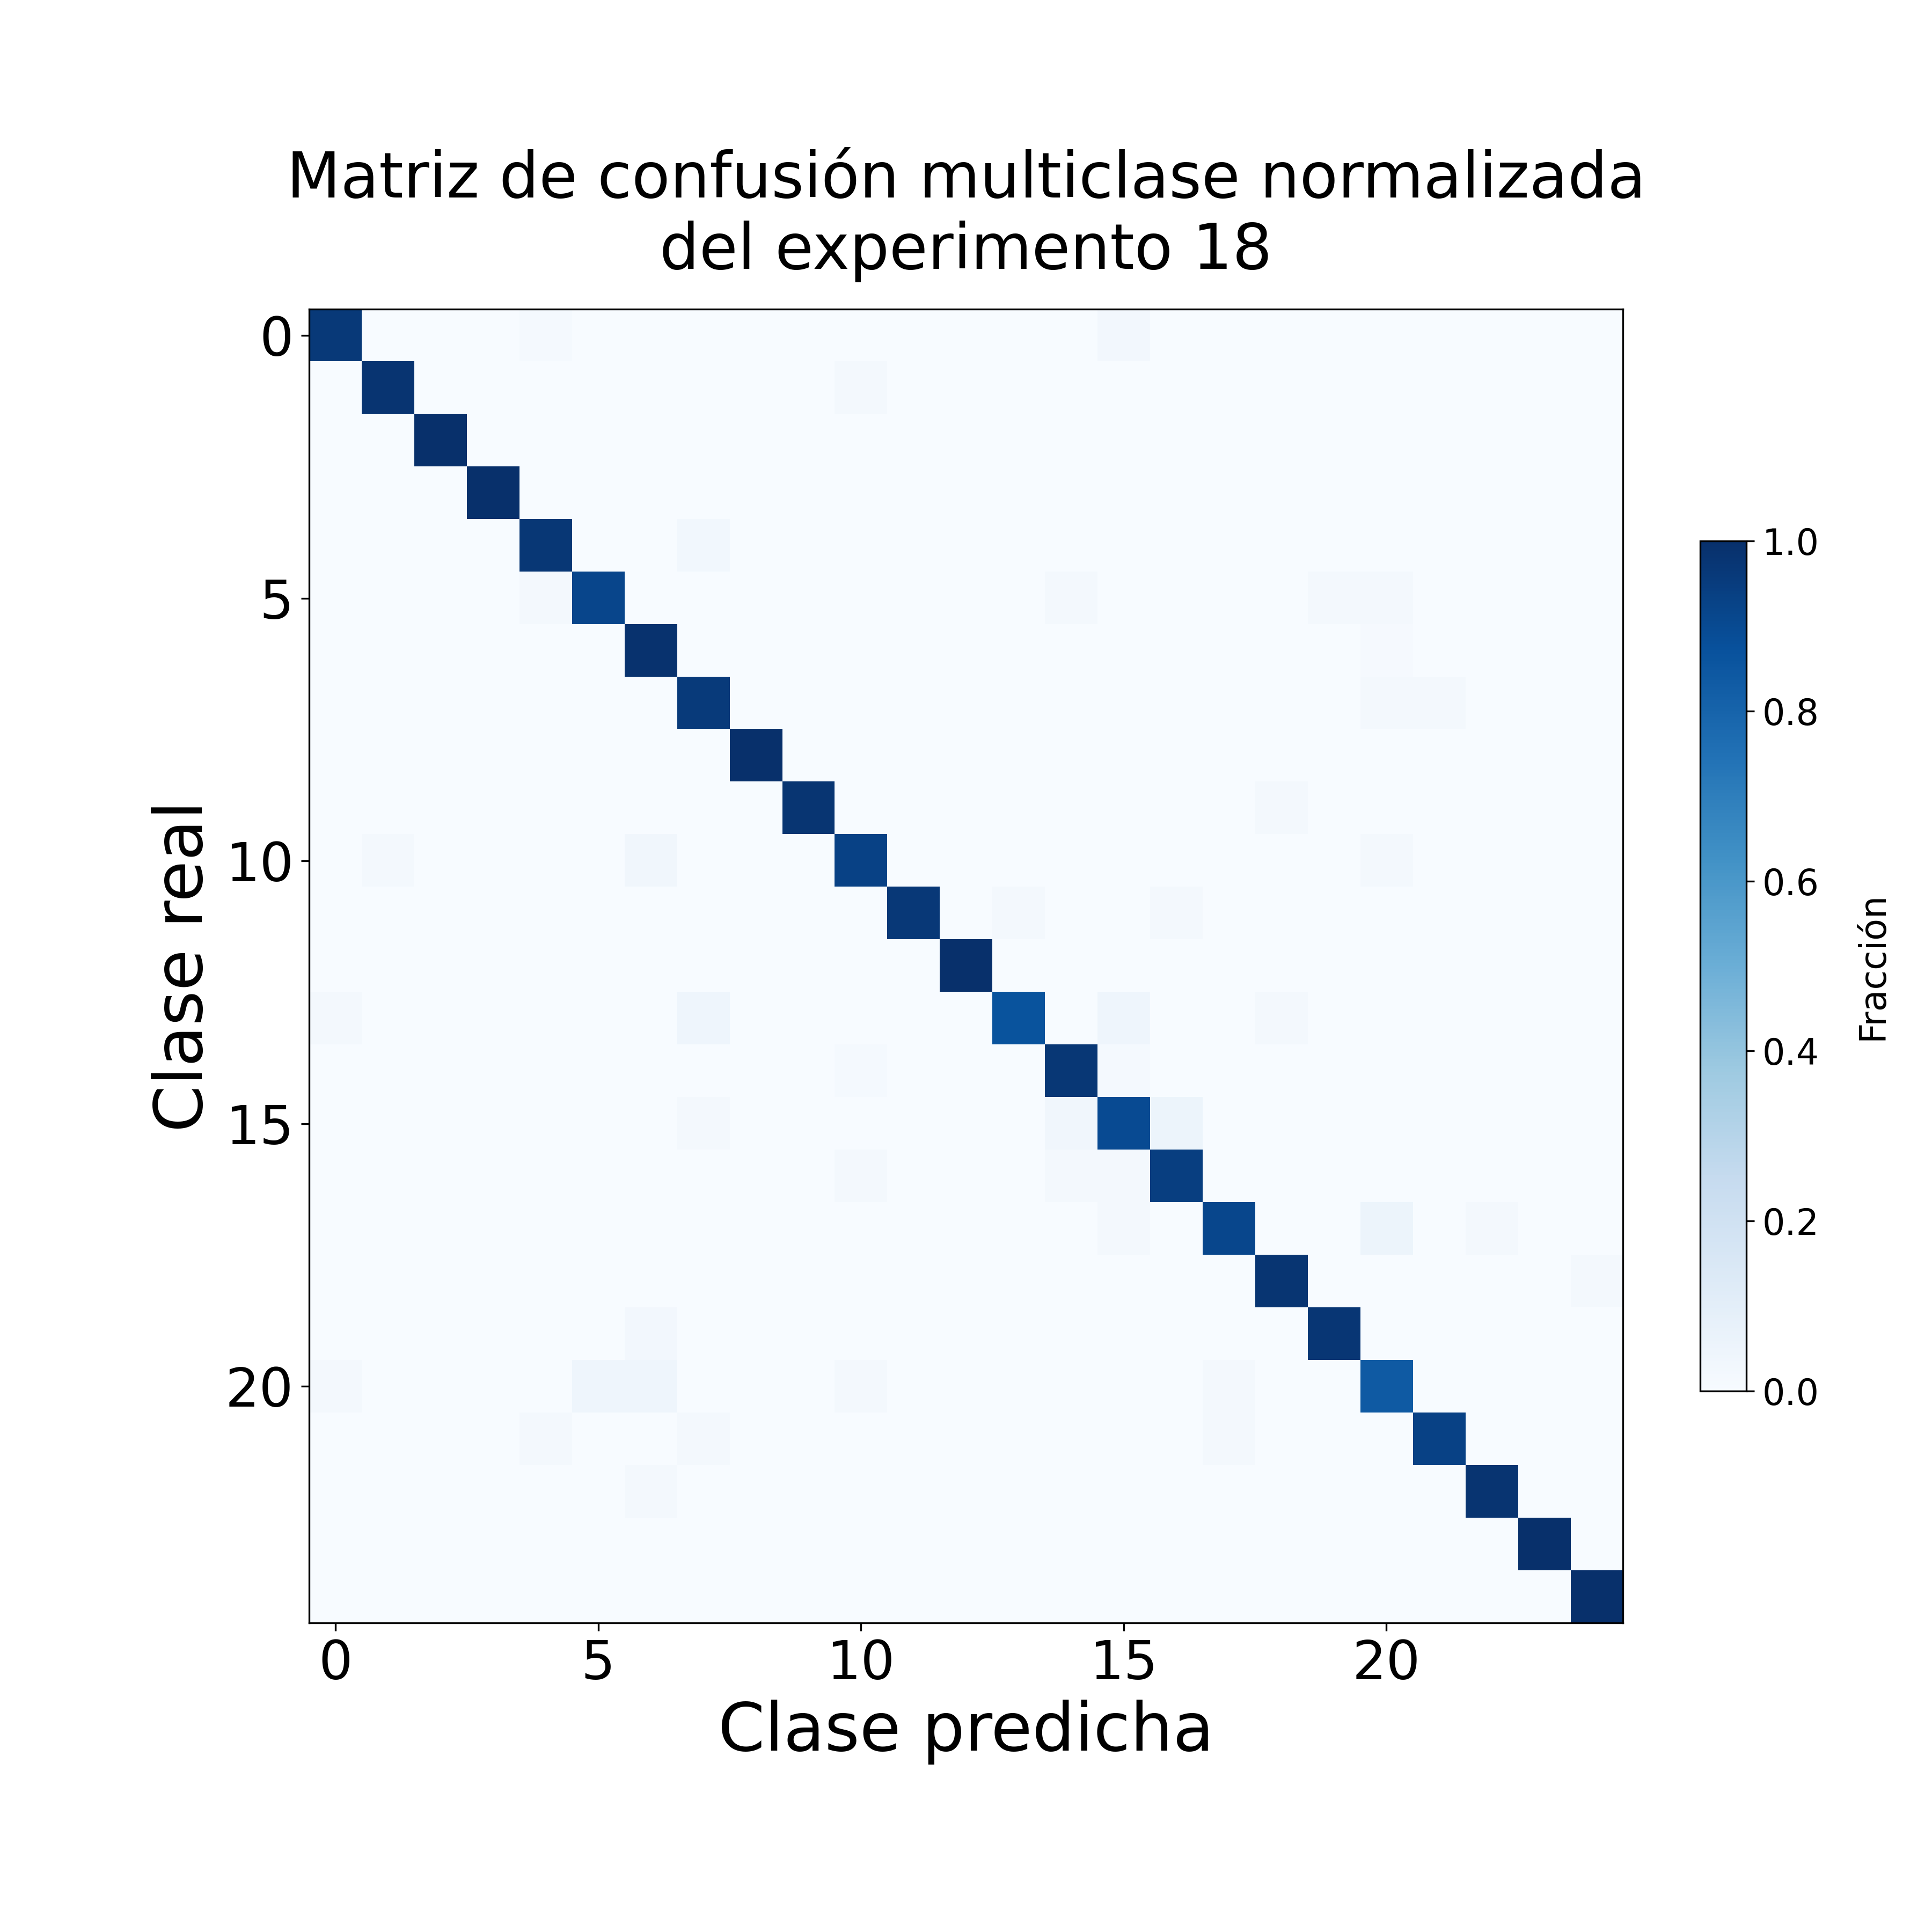
\includegraphics[width=\textwidth]{figures/Experiments_logs/confusion_matrix_05-14-1106.png}
        \caption{}
        \label{fig:confusion_matrix_05-14-1106}
    \end{subfigure}
    \hfill
    \begin{subfigure}{0.45\textwidth}
        \centering
        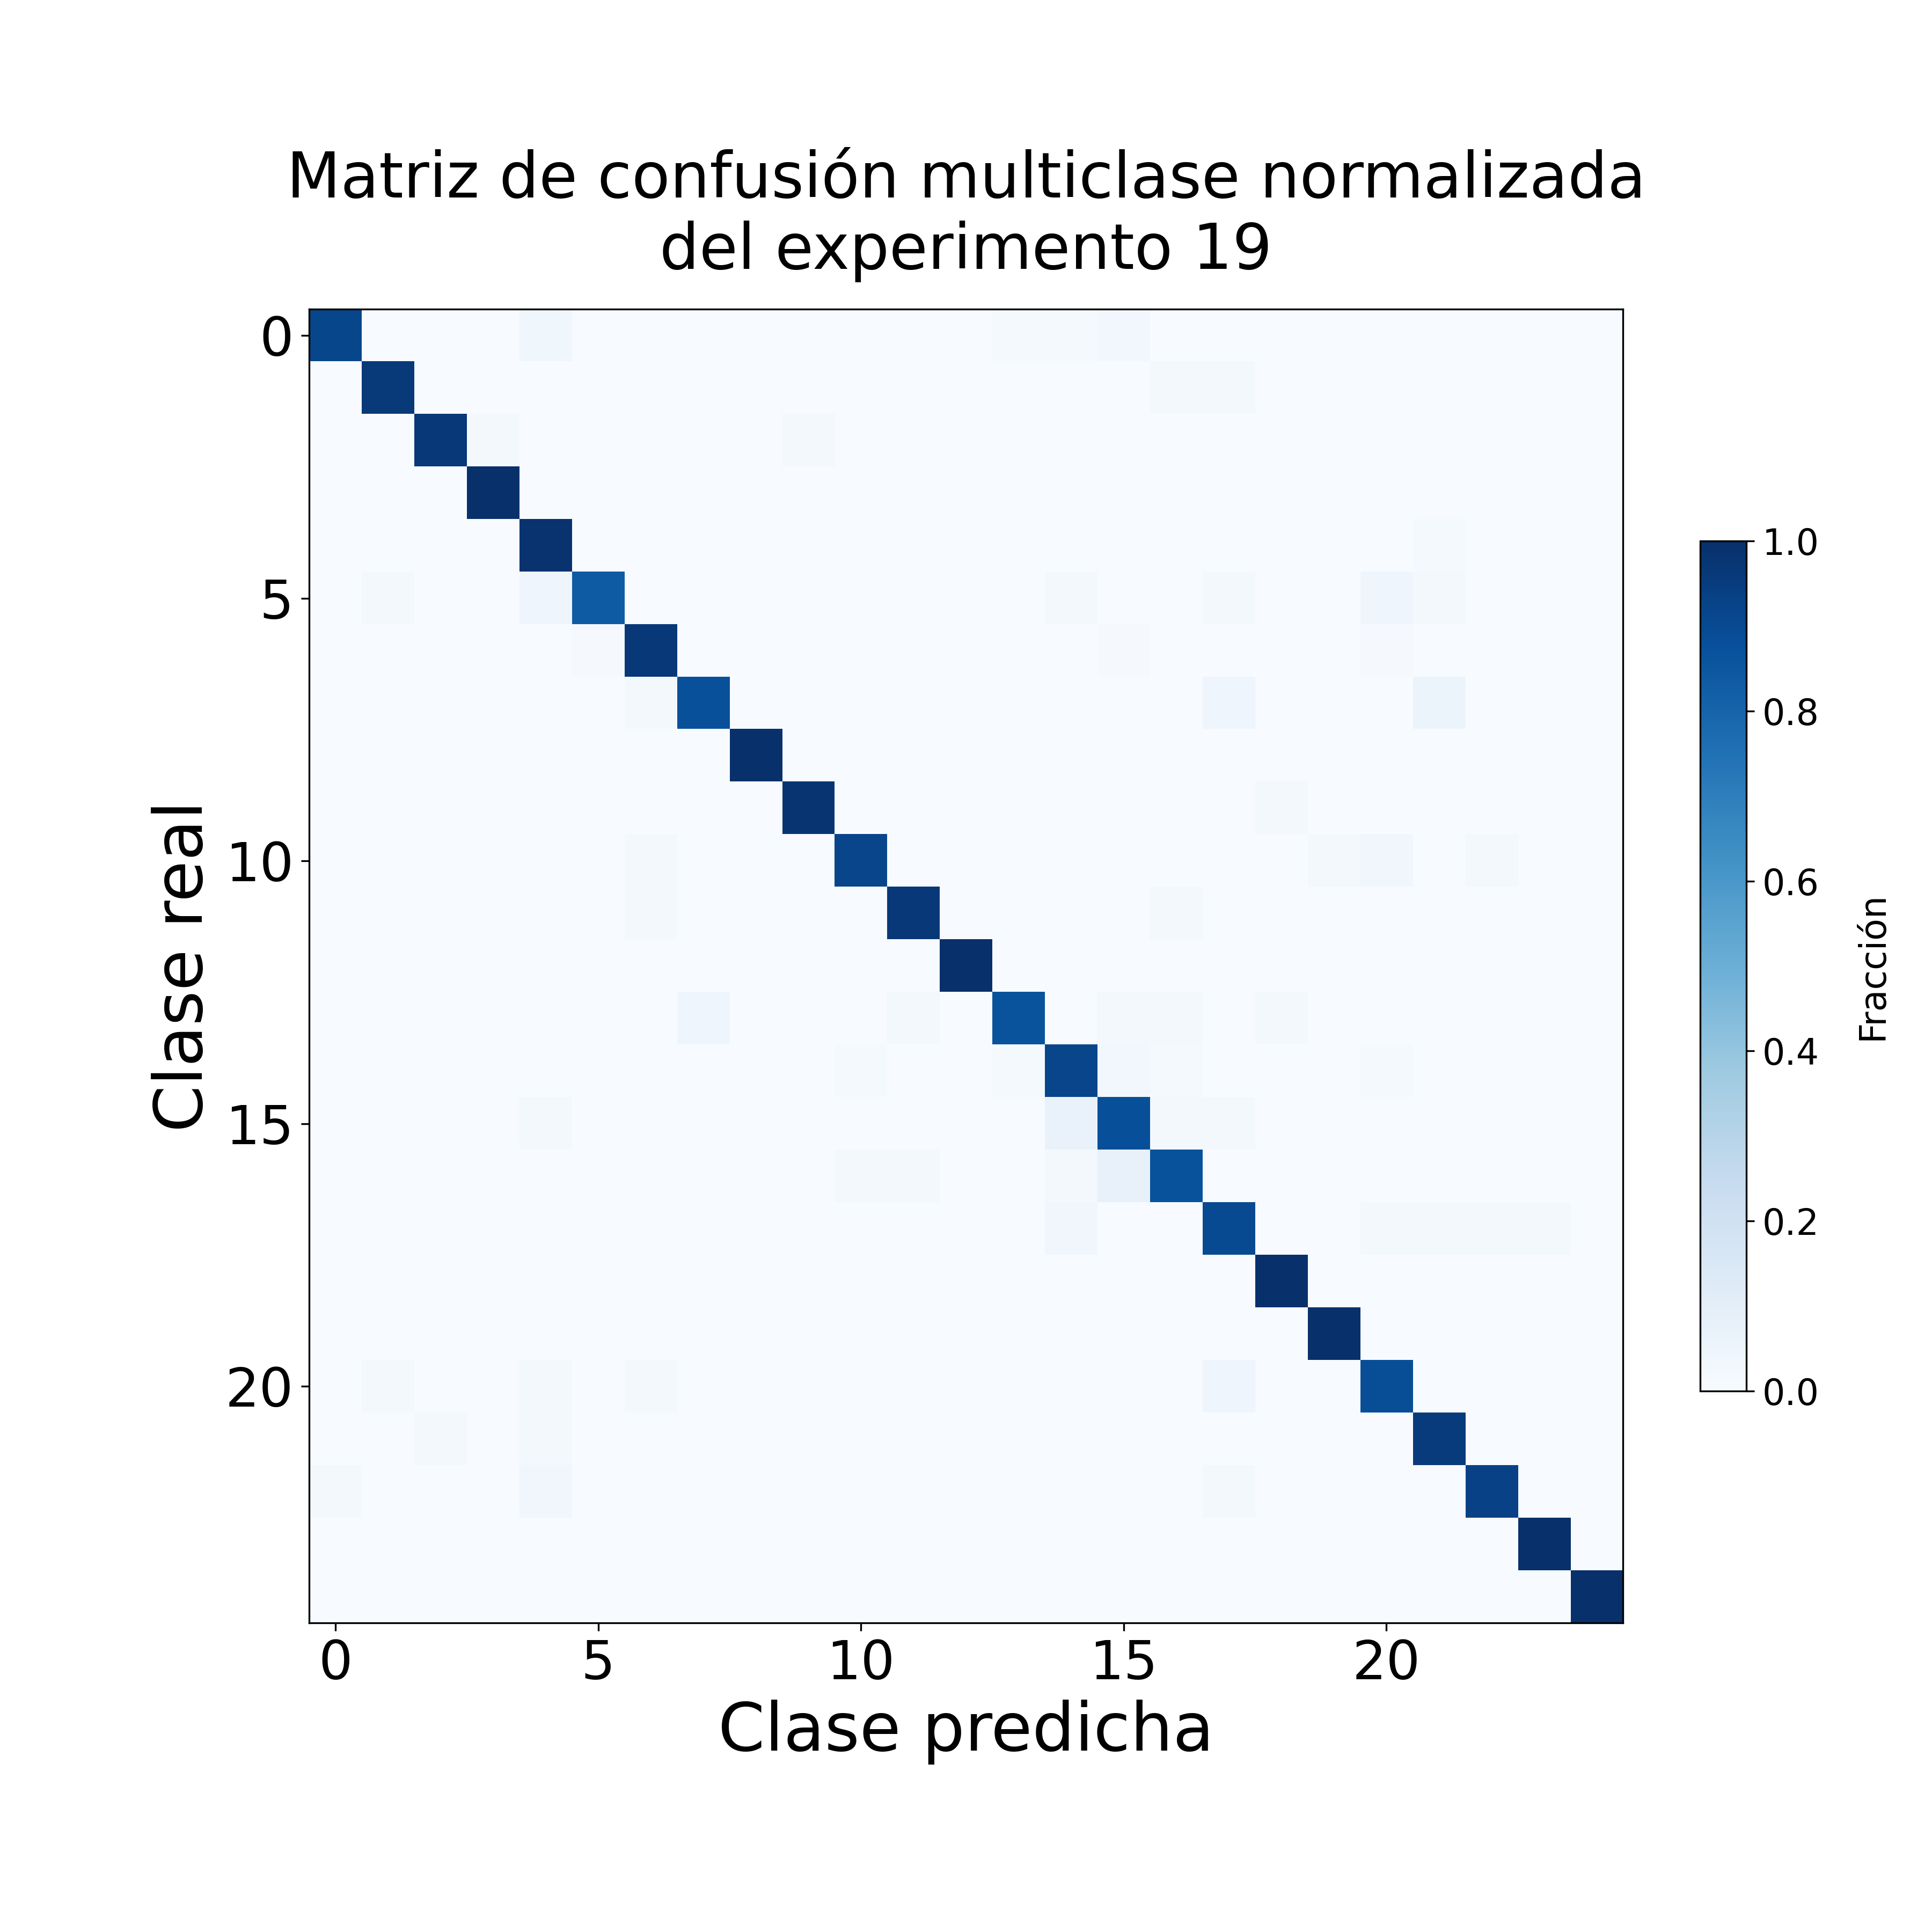
\includegraphics[width=\textwidth]{figures/Experiments_logs/confusion_matrix_05-14-1107.png}
        \caption{}
        \label{fig:confusion_matrix_05-14-1107}
    \end{subfigure}

    \caption{Matrices de confusión de los experimentos después de aplicar \textit{data augmentation}}
    \label{fig:confusion_matrix-05-14}
\end{figure}

Las matrices de confusión $\bigr($\figref{fig:confusion_matrix-05-14}$\bigl)$ muestran una diagonal muy marcada. Esto significa que el modelo clasifica correctamente la gran mayoría de los recortes. Los errores que quedan se concentran en clases visualmente parecidas. En el mejor experimento, las clases con F1 más bajo siguieron siendo algunas de las más difíciles del dataset, especialmente las relacionadas con objetos alargados o con geometría muy parecida.

El top-5 de 99,43\% también es importante. Quiere decir que, cuando el modelo no acierta la primera predicción, casi siempre tiene la clase correcta entre las cinco más probables. Esto sugiere que la representación aprendida por AIM + TTN contiene mucha información útil, aunque todavía haya confusiones finas entre clases muy similares.

La métrica \texttt{classification\_mAP} fue 98,41\%. Esta métrica se calculó como una media de precisión one-vs-rest sobre las probabilidades de clase. No debe confundirse con el \textit{mAP@50} de detección del paper de ChemEq25, porque aquí no se evalúan cajas ni IoU. Aun así, es una señal muy fuerte de que el ranking de probabilidades del clasificador es muy bueno.

\section{Variabilidad por seed y límite de las pruebas finales}

Después de alcanzar el 96,05\%, se lanzó una \textit{seed sweep} con la misma configuración para comprobar la robustez del modelo.

\begin{table}[H]
\centering
\small
\begin{tabular}{lccccc}
\toprule
\textbf{Experimento} & \textbf{Seed} & \textbf{Mejor acc.} & \textbf{Top-5} & \textbf{Macro F1} & \textbf{Acc. final} \\
\midrule
\texttt{20} & 17 & 92,96\% & 98,42\% & 92,88\% & 91,89\% \\
\texttt{21} & 88 & 93,40\% & 98,78\% & 93,41\% & 92,39\% \\
\texttt{22} & 123 & 92,25\% & 98,56\% & 92,33\% & 91,17\% \\
\texttt{23} & 314 & 93,54\% & 98,49\% & 93,57\% & 93,18\% \\
\midrule
\textbf{Media} & -- & \textbf{93,04\%} & -- & \textbf{93,05\%} & -- \\
\bottomrule
\end{tabular}
\caption{Seed sweep posterior al mejor resultado.}
\label{tab:seed_sweep}
\end{table}

Ninguno de los experimentos superó a \texttt{ChemEq\_exp15}. Todas quedaron entre 92,25\% y 93,54\%, por debajo del mejor experimento del 14 de mayo. Esto muestra que la \textit{seed} tiene un efecto fuerte.

También se probó aumentar la capacidad a \texttt{local\_dim=14} y \texttt{bond\_dim=14}, pero en esa prueba el resultado cayó a 88,16\%. Esto refuerza una idea importante: en este proyecto, más capacidad no siempre significa mejor generalización. Los cambios que más ayudaron fueron los que mejoraron la información visual y la regularización, no simplemente aumentar dimensiones.

\section{Resumen de la evolución experimental}

La evolución completa del proyecto se resume en la siguiente tabla:

\begin{table}[H]
\centering
\small
\begin{tabularx}{\textwidth}{lXc}
\toprule
\textbf{Fase} & \textbf{Cambio principal} & \textbf{Mejor accuracy} \\
\midrule
Flowers, CustomTTN inicial & TTN propia sin transformaciones intermedias & 3,58\% \\
Flowers, HybridCustomTTN & Transformaciones no lineales entre niveles & 13,60\% \\
Flowers, AIM + augmentation & Front-end AIM y aumento de datos & 33,96\% \\
ChemEq25 inicial & Cambio al dataset principal por crops & 57,00\% \\
ChemEq25 con LR menor & Optimización más estable & 75,23\% \\
ChemEq25 ajustado & Warmup, 12/12, regularización y label smoothing & 88,94\% \\
ChemEq25 final & \textit{Data augmentation light} y mejor seed & 96,05\% \\
\bottomrule
\end{tabularx}
\caption{Resumen global de la evolución experimental del proyecto.}
\label{tab:resumen_evolucion}
\end{table}

La lectura final es que el modelo basado en TN sí consiguió aprender una tarea visual real. El mejor resultado, 96,05\% de accuracy y 95,94\% de macro F1 en ChemEq25, demuestra que la arquitectura AIM + \texttt{HybridCustomTTN} es una alternativa viable para clasificación de imágenes de material de laboratorio.

\chapter{CONCLUSIONES}
\section{Conclusiones del trabajo}

El objetivo principal de este Trabajo de Fin de Grado era estudiar la aplicación de las \textit{Tensor Networks} en modelos de \textit{deep learning} para clasificación de imágenes. A partir del trabajo realizado, se puede concluir que este objetivo se ha cumplido de forma satisfactoria. El proyecto no se ha limitado a una revisión teórica de las redes tensoriales, sino que ha incluido el diseño, implementación, entrenamiento y evaluación de un modelo tensorial integrado en un \textit{pipeline} completo de clasificación.

En la parte teórica, el trabajo ha permitido establecer una base sólida sobre los conceptos necesarios para comprender este tipo de modelos, entre ellos los tensores, las contracciones, las descomposiciones tensoriales, la notación diagramática y topologías como MPS, TTN, PEPS o MERA. Esta fundamentación ha resultado clave para justificar las decisiones tomadas más adelante en la implementación, en especial la elección de una arquitectura jerárquica tipo TTN como núcleo del modelo desarrollado.

En el terreno computacional, se ha conseguido construir un sistema entrenable y reproducible basado en PyTorch y TensorKrowch. El proyecto abarca la carga y preparación de datos, el preprocesamiento de imágenes, la generación de recortes a partir de anotaciones YOLO, la definición de experimentos mediante archivos de configuración, el entrenamiento con GPU, el registro de métricas y la generación de diagnósticos. Esta organización ha permitido comparar configuraciones de manera ordenada y seguir la evolución del modelo a lo largo del desarrollo.

Una conclusión relevante es que las \textit{Tensor Networks}, concretamente para clasificación de imágenes, necesitan tener un buen tratamiento de datos e información, para que cuando entren en el modelo, le resulte más fácil diferenciar entre clases y mejorar las predicciones. Los primeros experimentos mostraron que una arquitectura tensorial aplicada directamente sobre representaciones simples tenía dificultades para generalizar. La incorporación de \texttt{AIMPatchEmbedding} permitió conservar mejor la información espacial de la imagen antes de entregarla a la TTN, y se convirtió en uno de los cambios clave para mejorar el comportamiento del entrenamiento.

El cambio al \textit{dataset} ChemEq25 también fue decisivo. A diferencia de Flowers102, que presentaba un número elevado de clases visualmente muy parecidas, ChemEq25 permitió abordar un problema más alineado con los objetivos del proyecto, la clasificación de material de laboratorio a partir de recortes individuales.

Los resultados experimentales muestran una mejora progresiva y coherente. El modelo pasó de unos resultados iniciales limitados a alcanzar un rendimiento elevado tras introducir mejoras en la representación de entrada, la optimización, la regularización y el \textit{data augmentation}. El mejor modelo, basado en la combinación de \texttt{AIMPatchEmbedding} y \texttt{HybridCustomTTN}, obtuvo un 96,05\% de \textit{accuracy}, un 95,94\% de F1 macro y un 99,43\% de \textit{top-5 accuracy} sobre ChemEq25. Estos valores indican que la arquitectura propuesta es capaz de aprender patrones visuales relevantes.

También se ha comprobado que aumentar la capacidad del modelo no garantiza por sí solo una mejor generalización. En los experimentos finales, los cambios que más contribuyeron al rendimiento fueron la preservación de la relación de aspecto, el \textit{label smoothing}, la regularización y, sobre todo, una estrategia suave de \textit{data augmentation}. Esto sugiere que, en modelos tensoriales aplicados a imágenes, la preparación de los datos y el control del entrenamiento pueden llegar a ser tan importantes como la propia topología de la red.

Entre las limitaciones, conviene señalar que no se ha realizado una comparación exhaustiva frente a arquitecturas convencionales como las CNN o los Transformers, ya que el objetivo principal era estudiar la viabilidad de las redes tensoriales, una línea que podría desarrollarse en trabajos posteriores. Asimismo, se ha observado cierta sensibilidad a la \textit{seed} y a la configuración de entrenamiento, lo que indica que estos modelos requieren una validación experimental cuidadosa.

En conjunto, el trabajo demuestra que las \textit{Tensor Networks} pueden integrarse de manera efectiva en modelos de \textit{deep learning} para clasificación de imágenes. Su aplicación práctica exige combinar la estructura tensorial con técnicas habituales del \textit{deep learning}, una representación visual adecuada y un seguimiento riguroso de los experimentos. La principal aportación del proyecto es, por tanto, mostrar un recorrido completo que va desde los fundamentos físicos y matemáticos de las redes tensoriales hasta un modelo funcional, entrenable y evaluable sobre datos reales.


\section{Conclusiones personales}

El desarrollo de este Trabajo de Fin de Grado ha supuesto una experiencia especialmente enriquecedora, tanto desde el punto de vista académico como personal. En primer lugar, el tema abordado pertenece a un ámbito muy especializado, las \textit{tensor networks}, cuyo funcionamiento requiere una comprensión profunda tanto de conceptos físicos como de herramientas computacionales avanzadas. Haber tenido la oportunidad de trabajar en este contexto, y de aprender bajo la supervisión de investigadores con experiencia en el área, en particular Alejandro Mata Ali y todo el departamento de computación cuántica del Instituto Tecnológico de Castilla y León, ha sido un privilegio y una parte fundamental del proceso formativo asociado a este trabajo.

A lo largo de estos meses, este TFG no solo me ha permitido profundizar en la física de las \textit{tensor networks}, sino también adquirir una gran cantidad de competencias técnicas que han resultado esenciales para el desarrollo del proyecto. Entre ellas, destaca el aprendizaje de Python a un nivel mucho más avanzado, así como la experiencia de programar desde cero un proyecto de cierta envergadura. Esto ha requerido no solo implementar código funcional, sino también aprender a organizarlo correctamente, aplicar buenas prácticas de programación y estructurar el trabajo de forma clara y mantenible.

Además, el proyecto ha supuesto un reto importante en el ámbito del \textit{machine learning}. Ha sido necesario familiarizarse con PyTorch, estudiar las bases matemáticas del \textit{deep learning} y comprender el flujo general de trabajo asociado a este tipo de modelos, desde la preparación de los datos hasta el entrenamiento y análisis de resultados. Todo ello ha ampliado considerablemente mi formación computacional y me ha permitido conectar herramientas modernas de inteligencia artificial con problemas propios de la física teórica y computacional.

Otro aspecto fundamental del desarrollo de este trabajo ha sido el aprendizaje de herramientas habituales en el entorno investigador. Durante el proyecto he aprendido a utilizar Git y GitHub para el control de versiones y la gestión del código, así como comandos básicos de Linux y Bash necesarios para trabajar de manera eficiente en los servidores de la universidad (Lorca). También he tenido la oportunidad de utilizar recursos de computación de alto rendimiento, que han sido clave para llevar a cabo los cálculos y entrenamientos necesarios. Esta experiencia me ha permitido comprender mejor cómo se organiza y ejecuta un proyecto computacional real en un entorno de investigación.

Más allá de los conocimientos técnicos, este TFG me ha acercado al funcionamiento cotidiano de la investigación científica. Haber podido participar en reuniones, observar la forma de trabajo del grupo y ver de primera mano cómo se plantean, discuten y desarrollan problemas de investigación ha sido una parte especialmente valiosa de la experiencia. En este sentido, el trabajo no solo ha consistido en resolver un problema concreto, sino también en aprender cómo se investiga, cómo se colabora y cómo se construye conocimiento en un contexto académico real.

En conjunto, este TFG ha representado un desafío constante. Por un lado, debido a la dificultad conceptual asociada a la física de las \textit{tensor networks}; por otro, por la exigencia técnica derivada de la programación, el uso de herramientas de aprendizaje automático y el trabajo en entornos computacionales avanzados. Sin embargo, precisamente esta combinación de retos ha hecho que el proceso sea especialmente formativo. En apenas unos meses he adquirido conocimientos y habilidades que al inicio del proyecto no imaginaba poder desarrollar, y considero que esta experiencia ha supuesto un punto de inflexión importante en mi formación como físico.

En definitiva, ha sido un proyecto muy ambicioso que ha puesto a prueba todos mis conocimientos sobre física aprendidos en la carrera y ha ampliado considerablemente esos conocimientos, mas especializados en la física computacional. También me ha permitido crecer a nivel científico, ya que he aprendido muchas herramientas que me servirán en mi carrera profesional.

\input{chapters/9_referencias}

\chapter{ANEXOS}\label{sec:anexos}

En este capítulo se recoge el material complementario del trabajo. En particular, se enlaza el repositorio público que contiene el código fuente completo del proyecto, con el que se pueden reproducir los experimentos descritos en la metodología.

Todo el código desarrollado para este Trabajo de Fin de Grado se encuentra disponible en un repositorio público de GitHub. El repositorio incluye un archivo \texttt{README} con las instrucciones necesarias para instalar las dependencias y reproducir los experimentos presentados en este documento.

El repositorio puede consultarse en la siguiente dirección:

\url{https://github.com/Manuel-Arenas-Sanchez/Tensor-Network-Model-In-Depp-Learning.git}

\clearpage
\thispagestyle{empty}
\vspace*{\fill}
\begin{center}
[PÁGINA INTENCIONADAMENTE EN BLANCO]
\end{center}
\vspace*{\fill}

% ============================================================================
% FIN
% ============================================================================
\end{document}
